% =============================================================================
%
% This is the LaTeX source code of the lecture notes.
%
%
% Author:   Blazej Bucha
% Year:     2022
% Contact:  blazej.bucha@stuba.sk
% Encoding: UTF-8
%
% =============================================================================






% LaTeX packages and main settings
% =============================================================================

\documentclass[a4paper,12pt]{book}
\usepackage[backend=biber,style=iso-authoryear,maxcitenames=2]{biblatex}
\usepackage[main=slovak]{babel}
\usepackage[utf8]{inputenc}
\usepackage[T1]{fontenc}
\usepackage{enumitem}
\usepackage{amsmath}
\usepackage{amssymb}
\usepackage{mathtools}
\usepackage{upgreek}
\usepackage{listings}
\usepackage{xcolor}
\usepackage{graphicx}
\usepackage{accsupp}
\usepackage{csquotes}
\usepackage{cancel}
\usepackage[width=0.95\textwidth,font=small]{caption}
\usepackage[unicode,
            pdfborder={0 0 0},
            colorlinks=true,
            urlcolor=blue,
            citecolor=blue,
            linkcolor=blue]{hyperref}
\usepackage[top=2.5cm, bottom=2.5cm, left=2.5cm, right=2.5cm]{geometry}
\linespread{1.2}
\let\MakeUppercase\relax
\raggedbottom

% =============================================================================






% Set up the "biblatex" package (see 
% "https://github.com/michal-h21/biblatex-iso690" for further detail)
% =============================================================================

% Add the bibtext file with the references
\addbibresource{references.bib}


% Replace "et al." by the Slovak "a kol."
\DefineBibliographyStrings{slovak}{ andothers = {a\addspace kol\adddot} }


% Change the default separators between the authors of the same bibtex entry.  
% In the main text, we want "a" between two authors.  In the "References" 
% section, we want ";" between all authors.
\DeclareDelimFormat{multinamedelim}{\addspace a \addspace}
\DeclareDelimFormat[bib]{multinamedelim}{\addsemicolon\space}
\DeclareDelimAlias[bib]{finalnamedelim}{multinamedelim}

% =============================================================================






% Define and set the style of code listings
% =============================================================================

% Define custom colours
\definecolor{comments}{rgb}{0.65, 0.65, 0.65}
\definecolor{strings}{rgb}{0.0, 0.3, 0.7}
\definecolor{linenumbers}{rgb}{0.5, 0.5, 0.5}
\definecolor{keywords}{rgb}{0.85, 0.0, 0.0}
\definecolor{backcolour}{rgb}{0.98, 0.98, 0.98}


% Define custom listing style
\lstdefinestyle{codestyle}
{
    backgroundcolor=\color{backcolour},
    commentstyle=\color{comments},
    keywordstyle=\color{keywords},
    numberstyle=\tiny\noncopynumber,
    columns=flexible,
    stringstyle=\color{strings},
    basicstyle=\ttfamily\footnotesize,
    breakatwhitespace=false,
    breaklines=true,
    captionpos=b,
    keepspaces=true,
    numbers=left,
    numbersep=5pt,
    showspaces=false,
    showstringspaces=false,
    showtabs=false,
    tabsize=2
}


% Defines a new command that ensures we can copy the source code from the
% compiled PDF without copying the line numbers
\newcommand{\noncopynumber}[1]
{
    \BeginAccSupp{method=escape,ActualText={}}
    #1
    \EndAccSupp{}
}


% Apply the custom listing style
\lstset{style=codestyle}


% It seems the "listings" package is not able to encode the nice special Slovak
% characters such as "á", "ľ", etc.  Next follows a brute force solution.
\lstset{
  literate={á}{{\'a}}1
           {ä}{{\" a}}1
           {č}{{\v c}}1
           {ď}{{d\kern-0.07cm\char39\kern-0.07cm}}1
           {é}{{\'e}}1
           {í}{{\'i}}1
           {ĺ}{{\'l}}1
           {ľ}{{l\kern-0.12cm\char39\kern-0.05cm}}1
           {ň}{{\v n}}1
           {ó}{{\'o}}1
           {ô}{{\^o}}1
           {ŕ}{{\'r}}1
           {š}{{\v s}}1
           {ť}{{t\kern-0.10cm\char39\kern-0.05cm}}1
           {ú}{{\'u}}1
           {ý}{{\'y}}1
           {ž}{{\v z}}1
           {Á}{{\'A}}1
           {Ä}{{\" A}}1
           {Č}{{\v C}}1
           {Ď}{{\v D}}1
           {É}{{\'E}}1
           {Í}{{\'I}}1
           {Ĺ}{{\'L}}1
           {Ľ}{{L\kern-0.12cm\char39\kern-0.00cm}}1
           {Ň}{{\v N}}1
           {Ó}{{\'O}}1
           {Ô}{{\^O}}1
           {Ŕ}{{\'R}}1
           {Š}{{\v S}}1
           {Ť}{{\v T}}1
           {Ú}{{\'U}}1
           {Ý}{{\'Y}}1
           {Ž}{{\v Z}}1
}


% Add the "as" keyword to the Python listings
\lstdefinelanguage{mypython}[]{Python}{morekeywords={as,True,False}}


% Caption title for listings
\renewcommand\lstlistingname{Zdrojový kód}

% =============================================================================






% Custom commands
% =============================================================================

\newcommand{\diff}{\mathrm d}
\newcommand{\DIFF}{\mathcal D}
\newcommand{\INT}{\mathcal I}
\newcommand{\grad}{\mathrm{grad}}
\newcommand{\divergence}{\mathrm{div}}
\newcommand{\gidx}{\mathrm g}
\newcommand{\cidx}{\mathrm c}
\let\vec\mathbf

% Let's change the "Dodatok" label of chapters after Conclusions to "Príloha"
\addto\captionsslovak{\renewcommand\appendixname{Príloha}}

% =============================================================================






% Custom hyphenation for some English words in a Slovak text
% =============================================================================

% Isn't there a more clever way to achieve the same?
\hyphenation{New-ton}
\hyphenation{New-to-nov}
\hyphenation{New-to-nom}
\hyphenation{New-to-no-va}
\hyphenation{New-to-nov-ho}
\hyphenation{New-to-no-vým}

% =============================================================================






% =============================================================================

\sloppy
\begin{document}

% -----------------------------------------------------------------------------

\chapter*{Predslov}

Mnohé geodetické úkony a~merania využívajú pôsobenie tiažového poľa Zeme alebo 
sú ním ovplyvnené, od použitia olovnice až po určovanie polohy pomocou 
globálnych navigačných družicových systémov.  Táto práca sa zaoberá tiažovým 
poľom s~dôrazom na geodetický kontext.  Určená je predovšetkým ako doplňujúci 
učebný text k~predmetom \emph{Fyzikálna geodézia~1} a~\emph{Fyzikálna 
geodézia~2} pre študentov odboru Geodézia a~kartografia Stavebnej fakulty 
Slovenskej technickej univerzity v~Bratislave.  Niektoré časti by azda mohli 
byť užitočné aj pre~študentov príbuzných vedných odborov alebo jednoducho pre 
záujemcov o~problematiku gravitačného a~tiažového poľa.

Popísané sú základné princípy gravitačného a~tiažového poľa vychádzajúce 
z~Newtonovho gravitačného zákona 
(Kapitola~\ref{sec:gravitational_and_gravity_field}), sférické a~sféroidické 
harmonické funkcie (Kapitoly~\ref{sec:spherical_harmonic_expansion} 
a~\ref{sec:spheroidal_harmonics_chapter}), normálne tiažové pole Zeme 
(Kapitola~\ref{sec:normal_gravity_field}), poruchové pole a~zvislicové odchýlky 
(Kapitola~\ref{sec:disturbing_field_deflections}) a~na záver geoid 
(Kapitola~\ref{sec:geoid}).  Hoci intelektuálne potešenie zo spoznávania týchto 
tém je bezodné, predsa len si vyžaduje pokročilé matematické zručnosti 
a~nepochybne aj~isté zanietenie.  Zvolili sme preto formu, ktorú na základe 
desaťročných skúseností s~výučbou fyzikálnej geodézie považujeme za 
najvhodnejšiu pre očakávaných čitateľov, študentov geodézie a~kartografie.  
Snažili sme sa o~výklad, ktorý by bol jednoduchý, zrozumiteľný, úplný, 
nápomocný a~súčasne i~podnecujúci.  Na miestach, kde sme to považovali za 
vhodné, text sme doplnili o~počítačový kód, ktorý prakticky demonštruje 
diskutovanú problematiku.  Nádejame sa, že jeho vlastným štúdiom, testovaním 
a~úpravou je možné niektorým konceptom porozumieť jednoduchšie.

Aj keď napísaniu tejto práce bolo venované veľké úsilie, bolo by prekvapivé, ak 
by sa v~nej nenašli časti, ktoré mohli byť spracované zrozumiteľnejšie, či 
témy, ktoré v~nej obsiahnuté nie sú, no mohli či mali byť diskutované.  Skôr 
než za uzavretý študijný podklad považujeme tento učebný text za živý 
zdokonaľujúci sa materiál.  Všetky zdrojové kódy sú preto voľne prístupné 
a~pripomienkovateľné na adrese 
\url{https://github.com/blazej-bucha/physical-geodesy-lecture-notes}.

Práca bola napísaná v~textovom editore Vim~v8.2 použitím typografického systému
\TeX.  Skompilovaná bola programom \texttt{pdfTex}~v3.14159265-2.6-1.40.21.
Mapy boli pripravené v~\texttt{GMT}~v6.1.1.  Obrázky boli zhotovené v~programe
\texttt{Inkscape}~v1.0.2.  Väčšina výpočtového kódu je napísaná
v~jazyku \texttt{Python}~v3.9.2 s~využitím modulov
\texttt{NumPy}~v1.20.3, \texttt{Matplotlib}~v3.5.0 a~\texttt{SciPy}~v1.7.3.
Časť výpočtov je napísaná~v~prostredí~MATLAB~R2021b.
S~týmito aplikáciami sme interagovali pod operačným systémom Debian GNU/Linux
11 (Bullseye).  S~výnimkou programu MATLAB ide o~slobodný voľne šíriteľný
software.  Vyslovujeme preto vďaku a~slová ocenenia veľkej komunite
excelentných programátorov za to, že poskytujú prvotriedny slobodný software.

Úprimné slová vďaky ale patria v~prvom rade blízkym, priateľom a~kolegom, ktorí 
mi pomáhali počas písania práce.  Ďakujem recenzentom, Petrovi Vajdovi z~Ústavu 
vied o~Zemi Slovenskej akadémie vied a~Josefovi Seberovi z~Astronomického 
ústavu Akadémie Vied Českej republiky, za ich ochotu a~venovaný čas.  Zuzane 
Minarechovej ďakujem za neúnavné viacnásobné čítanie textu a~za mnoho 
hodnotných postrehov a~korekcií.  Za cenné pripomienky k~forme a~k~štylistike 
veľmi ďakujem Eme Nogovej.  Jurajovi Janákovi a~Martinovi Pitoňákovi ďakujem za 
obsahové komentáre, ktoré mi pomohli lepšie formovať štruktúru a~obsah práce.  
Za povzbudivé slová a~za pozitívnu spätnú väzbu vďačím Palovi Zahorcovi.  Za 
mnohonásobné prečítanie, za hŕbu štylistických korektúr, za ochotu takmer rok 
počúvať o~témach, ktoré som práve spracovával a~za neutíchajúcu podporu ďakujem 
Saške.


\vspace{4ex}

\noindent V~Bratislave 12.~10.~2022 \hfill Blažej Bucha






% -----------------------------------------------------------------------------
\tableofcontents
\newpage
% -----------------------------------------------------------------------------






% -----------------------------------------------------------------------------

\chapter*{Úvod}
\label{sec:introduction}

Tvar Zeme možno definovať niekoľkými spôsobmi v~závislosti od kontextu 
\parencite{MoritzTheFigureOfTheEarth}.  Azda najprirodzenejšie je definovať 
tvar Zeme jej skutočným fyzickým povrchom, ktorý je viditeľný voľným okom.  
Tento povrch obsahuje nespočetné množstvo zložitých terénnych útvarov, 
napríklad strmé útesy či rokliny.  Hoci sú tieto oblasti krásne na pohľad, 
znemožňujú aplikáciu istej časti potrebného matematického aparátu, okrem iného 
plošnú integráciu.  Takto chápaný zemský povrch je preto spravidla skúmaný až 
po istom vyhladení.  Napriek vyhladeniu je to však stále veľmi zložitá plocha.

K~definovaniu tvaru Zeme môžeme pristúpiť aj~iným spôsobom.  Približne dve 
tretiny zemského povrchu tvorí voda v~podobe oceánov a~morí.  Za istých 
okolností existuje fyzikálna veličina, ktorá má na povrchu vodnej hladiny 
konštantnú hodnotou.  Táto vlastnosť by mohla umožniť akúsi predikciu morskej 
hladiny i popod, resp. ponad kontinenty.  V~porovnaní s~predošlým prístupom by 
sme tak získali geometricky jednoduchšiu a~hladšiu plochu, navyše aj s~istými 
relatívne jednoducho uchopiteľnými fyzikálnymi vlastnosťami.  Takáto definícia 
tvaru Zeme bola navrhnutá C.~F.~Gaussom~(1777--1855) a~podľa návrhu Gaussovho 
doktoranda J.~B.~Listinga~(1808--1882) nazývame túto plochu \emph{geoid}.  
Konštantnou veličinou na povrchu geoidu je \emph{tiažový potenciál}.

\emph{Fyzikálna geodézia} je vedná disciplína zaoberajúca sa určovaním tvaru 
Zeme, jej tiažovým poľom a~ich zmenami v~čase.  Študované sú oba vyššie opísané 
prístupy k~tvaru Zeme, pričom historicky bol predmetom záujmu ako prvý geoid.  
Matematicky odvážna myšlienka určovať priamo fyzický povrch Zeme pochádza už od 
E.~H.~Brunsa~(1848--1919), no do popredia záujmu ju dostal až 
M.~S.~Molodenskij~(1909--1991) v~polovici 20. storočia.  Aj~v~tomto prípade je 
však tvar Zeme určovaný z~informácie o~tiažovom poli.  Študovať tvar Zeme, čo 
je jedna zo základných úloh geodézie, teda znamená študovať aj tiažové pole 
Zeme.






% -----------------------------------------------------------------------------

\chapter{Gravitačné a~tiažové pole}
\label{sec:gravitational_and_gravity_field}






\section{Newtonov gravitačný zákon}
\label{sec:newton_law}

Dva hmotné body~$P$ a~$Q$ sa navzájom priťahujú \emph{gravitačnou silou}
%
\begin{equation}
\label{eq:newton_law}
\vec F_\gidx = -G \frac{m_P \, m_Q}{l^2} \, \frac{\vec r}{l}{.}
\end{equation}
%
Symbol~$G$ označuje gravitačnú konštantu, $m_P$ a~$m_Q$ predstavujú hmotnosti 
hmotných bodov, $\vec r$ je vektor definovaný polohou bodov~$P$ a~$Q$ so 
začiatkom v~bode~$Q$ a~$l$ je vzdialenosť medzi hmotnými bodmi, $l = \| \vec 
r \|$.  Záporné znamienko v~rovnici znamená, že vektor sily má začiatok v~bode 
$P$ a~smeruje do bodu~$Q$ (Obrázok~\ref{fig:newton_law}).

\begin{figure}[b]
\centering
\input{./fig-newton-law.pdf_tex}
%\captionsetup{width=0.8\textwidth}
\caption{Gravitačná sila~$\vec F_\gidx$ pôsobiaca medzi hmotnými bodmi~$Q$ 
a~$P$.  Vektor~$\vec F_\gidx$ je z~vizualizačných dôvodov mierne odsadený od 
spojnice bodov~$P$ a~$Q$.}
\label{fig:newton_law}
\end{figure}

Rovnica~(\ref{eq:newton_law}) sa nazýva \emph{gravitačný zákon} a~bola 
publikovaná I.~Newtonom (1642--1727) v~práci \emph{Philosophi\ae Naturalis 
Principia Mathematica} z~roku 1687.  Hovorí, že každý hmotný bod vo vesmíre 
priťahuje každý iný hmotný bod silou, ktorej veľkosť je priamo úmerná súčinu 
ich hmotností a~nepriamo úmerná štvorcu ich vzdialenosti.  Smer sily je daný 
spojnicou hmotných bodov \parencite{Kellogg1967}.  \emph{Hmotný bod} je 
idealizovaný pojem predstavujúci časticu s~nulovým rozmerom a~konečnou 
nenulovou hmotnosťou bez akýchkoľvek ďalších vlastností či štruktúry.  Hodnota 
gravitačnej konštanty odporúčaná od roku 2018 \emph{Komisiou pre dáta vo vede 
a~technológiách} (CODATA) je~$G = (6.67430 \pm 0.00015) \times 10^{-11} 
\ \mathrm{m}^3 \ \mathrm{kg}^{-1} \ \mathrm{s}^{-2}$.

Nech planéta obieha okolo Slnka (Obrázok~\ref{fig:orbital_motion}).  Označme 
polohu planéty v~čase~$t_0$ symbolom~$P(t_0)$ a~vektor jej okamžitej rýchlosti 
symbolom~$\vec v(t_0)$.  Predpokladajme, že planéta má v~čase~$t_0$ udelenú 
nenulovú rýchlosť, $\| \vec v(t_0) \| > 0$.  Ak by od času~$t_0$ nepôsobila na 
planétu žiadna sila, \emph{Newtonov pohybový zákon} hovorí, že planéta by sa 
ďalej pohybovala rovnomerným priamočiarym pohybom v~smere vektora~$\vec 
v(t_0)$.  Za istý čas by sa teda dostala do polohy~$P'(t_1)$.  Jediný spôsob 
ako zmeniť túto dráhu je pôsobiť na planétu silou.  
Z~rovnice~(\ref{eq:newton_law}) vyplýva, že Slnko pôsobí v~čase~$t_0$ na 
planétu gravitačnou silou~$\vec F_\gidx(t_0)$, ktorej smer je daný spojnicou 
planéty a~Slnka.  Gravitačná sila preto priťahuje planétu v~smere vektora~$\vec 
F_\gidx(t_0)$, čím mení hypotetickú trajektóriu, ktorou by sa planéta 
pohybovala bez pôsobenia tejto sily.  V~kombinácii s~vektorom rýchlosti tak 
gravitačná sila spôsobí, že planéta sa v~skutočnosti dostane do 
polohy~$P(t_1)$.  V~čase~$t_1$ sa opísaná situácia opakuje, pričom vektory 
rýchlosti a~sily už majú iný smer a~s~vysokou pravdepodobnosťou aj inú veľkosť.  
Gravitačná sila Slnka teda zakrivuje trajektóriu planéty \emph{v~každom 
okamihu}.

\begin{figure}
\centering
\input{./fig-orbital-motion-ideal.pdf_tex}
\caption{Obeh planéty okolo Slnka.}
\label{fig:orbital_motion}
\end{figure}

Newtonovým gravitačným zákonom je možné vysvetliť aj mnoho ďalších prírodných 
javov, napríklad príliv a~odliv, či zodpovedať otázku, prečo majú planéty 
približne sférický tvar.  Je pozoruhodné, že hoci rovnica~(\ref{eq:newton_law}) 
bola odpozorovaná z~pohybu nebeských telies, zhoduje sa i~s experimentmi, ktoré 
boli vykonané na vzdialenosť niekoľkých desiatok mikrometrov 
\parencite{Lee2020}.  Napriek uvedenému je azda potrebné spomenúť 
aj~skutočnosť, že Newtonov gravitačný zákon je \emph{nesprávny} 
\parencite{Feynman}.  Predpokladá napríklad, že zmena hmotnosti či vzdialenosti 
má okamžitý gravitačný účinok, a~to aj~v~prípade telies nachádzajúcich sa vo 
veľkých vzdialenostiach.  Tento predpoklad je ale v~rozpore s~experimentálne 
potvrdenou Einsteinovou špeciálnou teóriou relativity.  Tá hovorí, že žiadny 
signál, ani gravitačný, sa nemôže šíriť rýchlosťou väčšou ako je rýchlosť 
svetla.  Pre účely fyzikálnej geodézie sú však nepresnosti Newtonovho 
gravitačného zákona väčšinou zanedbateľné.  Newtonova teória gravitácie tak aj 
dnes, viac ako tristo rokov po jej vzniku, tvorí chrbtovú kosť fyzikálnej 
geodézie.






\subsection{Gravitačné zrýchlenie}
\label{sec:gg}

Gravitačná sila~(\ref{eq:newton_law}) pôsobiaca medzi hmotnými bodmi~$P$ 
a~$Q$~závisí od hmotnosti oboch hmotných bodov.  Vektor gravitačnej sily je 
preto výhodné normovať hmotnosťou~$m_P$.  Získame tým vektorovú veličinu, ktorú 
budeme nazývať \emph{gravitačné zrýchlenie},
%
\begin{equation}
\label{eq:gg_point_mass}
\vec g_\gidx(P) = \frac{\vec F_\gidx}{m_P} = -G \frac{m}{l^2} \, \frac{\vec
r}{l}{,}
\end{equation}
%
kde~$m = m_Q$.  Rovnica~(\ref{eq:gg_point_mass}) hovorí, že hmotný
bod~$Q$ udeľuje hmotnému bodu~$P$ zrýchlenie~$\vec g_\gidx(P)$.   Inými
slovami, gravitačné zrýchlenie~$\vec g_\gidx(P)$ nezávisí od hmotnosti~$m_P$, 
začiatok má v~bode~$P$ a~smeruje do hmotného bodu~$Q$.  V~súvislosti
s~hmotným bodom~$P$ je preto možné pre jednoduchosť vynechať prívlastok
\emph{hmotný} a~považovať~$P$ za geometrický bod bez fyzikálnych vlastností.
Skutočnosť, že gravitačné zrýchlenie priťahovaného telesa nezávisí od jeho
hmotnosti experimentálne potvrdil Gaileo Gailei (1564--1642).

Popíšme teraz vektor gravitačného zrýchlenia v~sústave~$N$ hmotných bodov 
(Obrázok~\ref{fig:gg_n_point_masses}).  Keďže \uv{\textit{[\dots] každý hmotný 
bod [\dots] priťahuje každý iný hmotný bod [\dots]}} (pozri 
Kapitolu~\ref{sec:newton_law}), celkové gravitačné zrýchlenie v~bode~$P$ je 
dané vektorovým súčtom čiastkových gravitačných zrýchlení, ktoré sú generované 
jednotlivými hmotnými bodmi.  Tento princíp sa nazýva \emph{princíp 
superpozície} \parencite[pozri napríklad][]{Hotine}.  Gravitačné zrýchlenie 
generované~$N$ hmotnými bodmi tak získame vzťahom
%
\begin{equation}
\label{eq:gg_N_point_masses}
\vec g_\gidx(P) = \sum_{i = 1}^{N}\vec g_{\gidx,i}(P) = -G \sum_{i = 1}^{N}
\frac{m_i}{l_i^2} \, \frac{\vec r_i}{l_i}{.}
\end{equation}

\begin{figure}
\centering
\input{./fig-gg-n-point-masses.pdf_tex}
\caption{Gravitačné zrýchlenie~$\vec g_\gidx$ v~bode~$P$ generované sústavou 
piatich hmotných bodov~$Q_1$ až~$Q_5$ s~rôznou hmotnosťou a~polohou voči 
bodu~$P$.  Vektor~$\vec g_\gidx$ je daný vektorovým súčtom čiastkových 
gravitačných zrýchlení~$\vec g_{\gidx,1}$ až~$\vec g_{\gidx,5}$, ktoré sú 
generované príslušnými hmotnými bodmi.}
\label{fig:gg_n_point_masses}
\end{figure}

Newtonov gravitačný zákon~(\ref{eq:newton_law}) 
a~rovnice~(\ref{eq:gg_point_mass}) a~(\ref{eq:gg_N_point_masses}) platia iba 
pre hmotné body.  V~tomto tvare môžu byť aplikované napríklad na popis pohybov, 
ktoré vykonávajú planéty Slnečnej sústavy.  Rozmery planét sú totiž natoľko 
zanedbateľné v~porovnaní s~ich vzájomnou vzdialenosťou, že sa nedopustíme 
nerozumne veľkej chyby, ak hmotnosti planét sústredíme do ich ťažísk 
a~zanedbáme tvar planét.  Menej priaznivá situácia nastáva vtedy, keď sa 
bod~$P$ nachádza v~blízkosti priťahujúceho telesa, ktoré má komplikovaný tvar 
a~hustotu.  Príkladom je družica na nízkej obežnej dráhe Zeme.  Na získanie 
výsledného gravitačného zrýchlenia, ktoré Zem udeľuje družici, opäť využijeme 
princípe superpozície, teda sčítame individuálne gravitačné vplyvy spôsobené 
jednotlivými časťami Zeme.  Tentokrát si už ale nevystačíme s~konceptom 
hmotných bodov (rovnica~\ref{eq:gg_N_point_masses}), pretože tie sme definovali 
ako bezrozmerné (Kapitola~\ref{sec:newton_law}).  Bezrozmernými hmotnými bodmi 
nedokážeme aproximovať nenulový objem priťahujúceho telesa.

Zaveďme pojem \emph{všeobecné teleso}.  Všeobecné teleso má konečný 
objem~$\tau$ a~jeho hustota~$\rho$ je ohraničenou funkciou polohy 
(Obrázok~\ref{fig:gravitating_body}).  V~zmysle integrálneho počtu rozdeľme 
všeobecné teleso na diferenciálne hmotné elementy~$\diff m$, pričom
%
\begin{equation}
\label{eq:dm}
\diff m = \rho \, \diff \tau{.}
\end{equation}
%
Hustota $\rho$ sa môže meniť medzi diferenciálnymi hmotnými elementmi~$\diff m$ 
v~závislosti od štruktúry telesa, ale nesmie sa meniť v~rámci elementu 
samotného.  Ďalej budeme predpokladať, že hmota diferenciálneho elementu~$\diff 
m$ je koncentrovaná v~niektorom bode elementu \parencite{Kellogg1967}.  Po 
uvážení rovnice~(\ref{eq:dm}) je diferenciál gravitačného zrýchlenia 
generovaného diferenciálnym hmotným elementom~$\diff m$ daný vzťahom (porovnaj 
so vzťahom~\ref{eq:gg_point_mass})
%
\begin{equation}
\label{eq:gg_dm}
\diff \vec g_\gidx(P) = -G \frac{\vec r}{l^3} \, \diff m = -G \frac{\vec 
r}{l^3} \rho \, \diff\tau{,}
\end{equation}
%
kde vektor~$\vec r$ je definovaný rozdielom polohových vektorov bodov~$P$
a~$Q$,
%
\begin{equation}
\label{eq:r}
\vec r =
%
\begin{bmatrix}
x - x_Q \\
y - y_Q \\
z - z_Q
\end{bmatrix}
{,}
\end{equation}
%
a~$l = \| \vec r \|$ je jeho veľkosť, teda Euklidovská vzdialenosť medzi bodmi
$P$ a~$Q$,
%
\begin{equation}
\label{eq:l}
l = \sqrt{(x - x_Q)^2 + (y - y_Q)^2 + (z - z_Q)^2}{.}
\end{equation}

\begin{figure}
\centering
\input{./fig-gravitating-body.pdf_tex}
\caption{Všeobecné teleso.}
\label{fig:gravitating_body}
\end{figure}

Pri aplikovaní Newtonovho gravitačného zákona na diferenciálne hmotné elementy 
treba mať na pamäti, že tento zákon bol formulovaný pre hmotné body, nie pre 
diferenciálne hmotné elementy.  Diferenciálne elementy~$\diff m$, akokoľvek sú 
malé, nikdy nie sú identické s~hmotnými bodmi.  Inými slovami, Newtonov 
gravitačný zákon neposkytuje spôsob výpočtu gravitačného účinku diferenciálneho 
hmotného elementu \parencite{Kellogg1967}.  Budeme preto musieť vysloviť ďalší 
predpoklad, a~síce že tento zákon je možné aplikovať aj na diferenciálne hmotné 
elementy, čím získame rovnosť~(\ref{eq:gg_dm}).

Celkové gravitačné zrýchlenie generované všeobecným telesom získame
využitím princípu superpozície, teda integráciou vzťahu~(\ref{eq:gg_dm}),
%
\begin{equation}
\label{eq:gg_body}
\vec g_\gidx(P) = -G \iiint\limits_{\tau} \frac{\vec r}{l^3} \, \rho \, 
\diff\tau{.}
\end{equation}
%
Rovnica~(\ref{eq:gg_body}) už môže byť korektne použitá na výpočet gravitačného 
zrýchlenia všeobecného telesa (napríklad Zeme) v~ľubovoľnom bode~$P$ (napríklad 
v~ťažisku družice), pretože správne zohľadňuje tvar telesa a~rozloženie jeho 
hustoty.

Vektor gravitačného zrýchlenia je v~širšom zmysle možné odmerať, preto má pre 
fyzikálnu geodéziu kľúčový význam.  V~sústave jednotiek SI má 
jednotku~$\mathrm{m}\ \mathrm{s}^{-2}$.  Veľmi často sa stretneme aj 
s~jednotkou~$1\ \mathrm{Gal} = 10^{-2}\ \mathrm{m}\ \mathrm{s}^{-2}$, ktorá je 
pomenovaná podľa Galilea Galileiho, prípadne s~jej násobkami~$1\ \mathrm{mGal} 
= 10^{-5}\ \mathrm{m}\ \mathrm{s}^{-2}$ a~$1\ \upmu \mathrm{Gal} = 10^{-8}\ 
\mathrm{m}\ \mathrm{s}^{-2}$.

Obrázok~\ref{fig:gg_grav_sr_2arcsec} zobrazuje priebeh veľkosti vektora 
gravitačného zrýchlenia v~oblasti Vysokých a~Nízkych Tatier.  Z~globálneho 
hľadiska je gravitačné zrýchlenie ovplyvnené najmä tvarom Zeme, jej hmotnosťou, 
sploštením a~rozsiahlymi hustotnými celkami v~jej vnútri.  Na regionálnej 
úrovni možno pozorovať silnú závislosť medzi topografiou 
(Obrázok~\ref{fig:h_grav_sr_2arcsec}) a~veľkosťou vektora gravitačného 
zrýchlenia (Obrázok~\ref{fig:gg_grav_sr_2arcsec}).  Vidíme napríklad, 
že~miestach s~veľkou nadmorskou výškou je veľkosť gravitačného zrýchlenia 
spravidla menšia ako v~miestach s~malou nadmorskou výškou a~naopak.

\begin{figure}
\centering
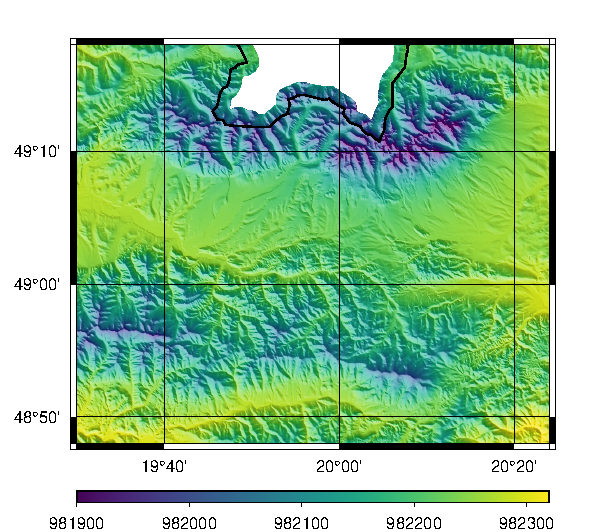
\includegraphics{./fig-gg-grav-sr-2arcsec.pdf}
\caption{Veľkosť vektora gravitačného zrýchlenia~$\| \vec g_\gidx \|$ na 
zemskom povrchu v~oblasti Vysokých a~Nízkych Tatier (jednotky mGal).  Dáta sú 
prevzaté z~modelu \texttt{grav-sr-2arcsec} \parencite{GravSR2arcsec}.}
\label{fig:gg_grav_sr_2arcsec}
\end{figure}

\begin{figure}
\centering
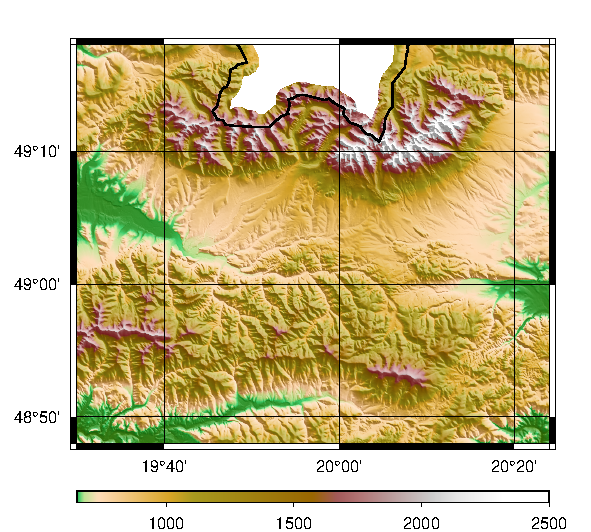
\includegraphics{./fig-h-grav-sr-2arcsec.pdf}
\caption{Topografia v~oblasti Vysokých a~Nízkych Tatier vyjadrená pomocou 
elipsoidickej výšky (jednotky~m).  Dáta sú prevzaté z~modelu 
\texttt{grav-sr-2arcsec} \parencite{GravSR2arcsec}.}
\label{fig:h_grav_sr_2arcsec}
\end{figure}







\subsection{Gravitačný potenciál}
\label{sec:vg}

Gravitačné zrýchlenie je vektorová veličina, ktorá má v~každom bode definovanú 
trojicu reálnych čísel.  V~niektorých situáciách je výhodnejšie pracovať so 
skalárnou veličinou, teda takou, ktorá má v~každom bode definované práve jedno 
reálne číslo.  Tento prístup je mladší ako Newtonov gravitačný zákon zhruba 
o~jedno storočie \parencite{MacMillan1930,Jekeli2015}.  Fenomén gravitácie 
chápe ako \emph{pole}, ktorého vlastnosti môžu byť popísané rôznymi vzájomne 
súvisiacimi veličinami.  Podľa \textcite{MacMillan1930} prišiel s~konceptom 
potenciálu poľa taliansky matematik a~astronóm J.~L.~Lagrange~(1736--1813).  Ak 
by sme našli skalárnu veličinu gravitačného poľa, informáciu poskytnutú troma 
číslami v~podobe gravitačného vektora by sme dokázali zredukovať na jedno 
jediné číslo bez straty informácie o~poli samotnom.  Skalárna veličina 
gravitačného poľa sa nazýva \emph{gravitačný potenciál} a~označuje sa 
symbolom~$V_\gidx$.

Gravitačný potenciál definujeme pomocou gravitačného zrýchlenia.  Pre lepšie 
pochopenie vzťahu medzi oboma veličinami však najprv predstavíme diferenciálny 
operátor gradient a~až následne pristúpime k~samotnej definícii gravitačného 
potenciálu.

\subsubsection{Operátor gradient v~karteziánskom súradnicovom systéme}

\emph{Operátor gradient} je v~trojrozmernom karteziánskom súradnicovom 
systéme~$x$, $y$, $z$ definovaný vzťahom
%
\begin{equation}
\label{eq:gradient}
\nabla = \grad = \vec e_1 \frac{\partial}{\partial x} + \vec e_2
\frac{\partial}{\partial y} + \vec e_3 \frac{\partial}{\partial z} =
\begin{bmatrix}
\dfrac{\partial}{\partial x} \\[2ex]
\dfrac{\partial}{\partial y} \\[2ex]
\dfrac{\partial}{\partial z}
\end{bmatrix}
{,}
\end{equation}
%
kde~$\vec e_1$, $\vec e_2$, $\vec e_3$ sú jednotkové vektory
rovnobežné so smerom súradnicových osí (Obrázok~\ref{fig:3d_coord_system}),
%
\begin{equation}
\label{eq:unit_vectors}
\vec e_1 =
\begin{bmatrix}
1\\
0\\
0\\
\end{bmatrix}
{,} \quad
%
\vec e_2 =
\begin{bmatrix}
0\\
1\\
0
\end{bmatrix}
%
{,}\quad
%
\vec e_3 =
\begin{bmatrix}
0\\
0\\
1
\end{bmatrix}
{,}
\end{equation}
%
\begin{equation}
\label{eq:unit_vectors_unit_length}
\| \vec e_i \| = 1{,} \quad i = 1, 2,3{.}
\end{equation}

Po aplikovaní operátora gradient na \emph{skalárnu} diferencovateľnú 
funkciu~$f$ získame \emph{vektorovú} funkciu,
%
\begin{equation}
\nabla f = \grad \ f = \vec e_1 \frac{\partial f}{\partial x} + \vec e_2 
\frac{\partial
f}{\partial y} + \vec e_3 \frac{\partial f}{\partial z} =
\begin{bmatrix}
\dfrac{\partial f}{\partial x} \\[2ex]
\dfrac{\partial f}{\partial y} \\[2ex]
\dfrac{\partial f}{\partial z}
\end{bmatrix}
{.}
\end{equation}
%
Vektor~$\nabla f(x, y, z)$ udáva \emph{smer a~veľkosť najväčšieho nárastu} 
funkcie~$f$ v~bode so súradnicami~$x$, $y$, $z$.  Jeho zložky popisujú zmenu 
skalárnej funkcie~$f$ v~smere vektorov~$\vec e_1$, $\vec e_2$, $\vec e_3$ 
v~bode~$x$, $y$, $z$.

Operátor gradient je \emph{lineárny}, teda pre diferencovateľné funkcie~$f$ 
a~$g$ a~konštantu~$c$ platí
%
\begin{align}
\label{eq:gradient_additivity}
\nabla \left(f + g \right) &= \nabla f + \nabla g{,}\\
%
\label{eq:gradient_homogenity}
\nabla (c \, f) &= c \, \nabla f{.}
\end{align}

Numerická ukážka aplikácie operátora gradient je uvedená 
v~Prílohe~\ref{app:numerical_application_of_gradient}.

\begin{figure}
\centering
\input{./fig-3d-coord-system.pdf_tex}
\caption{Trojrozmerný karteziánsky súradnicový systém a~jednotkové vektory.}
\label{fig:3d_coord_system}
\end{figure}

\subsubsection{Definícia gravitačného potenciálu}

Gravitačný potenciál je skalárna funkcia, ktorá vyhovuje rovnici 
\parencite{SansoGeoidDetermination}
%
\begin{equation}
\label{eq:gg_grad_vg}
\vec g_\gidx(P) = \nabla V_\gidx(P)
\end{equation}
%
a~spĺňa podmienku
%
\begin{equation}
\label{eq:vg_at_infty}
\lim_{P \to \infty} V_\gidx(P) = 0{.}
\end{equation}
%
Vzťah~(\ref{eq:gg_grad_vg}) hovorí, že vektor gravitačného zrýchlenia udáva 
smer a~veľkosť najväčšieho nárastu gravitačného potenciálu.  
Rovnica~(\ref{eq:vg_at_infty}) znamená, že v~nekonečnej vzdialenosti od telesa 
nadobúda gravitačný potenciál nulovú hodnotu.  Tento vzťah zabezpečuje, že 
existuje práve jedna funkcia~$V_\gidx$, ktorá vyhovuje 
rovnici~(\ref{eq:gg_grad_vg}) \parencite{SansoGeoidDetermination}.

Poznamenajme, že bod s~nulovým gravitačným potenciálom je možné vybrať 
ľubovoľne, čo však neznamená, že jeho voľba je nedôležitá.  Naopak, miesto 
nulového gravitačného potenciálu ovplyvňuje hodnoty gravitačného potenciálu.  
Hovoríme preto, že \emph{gravitačný potenciál je relatívna veličina}.  Často je 
preto dôležitejšie poznať relatívne vzťahy medzi gravitačným potenciálom 
v~priestore, napríklad rozdiel potenciálu medzi dvoma bodmi, než je potrebné 
poznať absolútnu hodnotu gravitačného potenciálu v~niektorom bode.

Gravitačný potenciál hmotného bodu je daný vzťahom
%
\begin{equation}
\label{eq:vg_point_mass}
V_\gidx(P) = \frac{G \, m}{l}{.}
\end{equation}
%
Overme, či tento vzťah vyhovuje rovniciam~(\ref{eq:gg_grad_vg})
a~(\ref{eq:vg_at_infty}).  Aplikujme operátor gradient~(\ref{eq:gradient})
na gravitačný potenciál~(\ref{eq:vg_point_mass}).  S~využitím 
rovnice~(\ref{eq:l}) dostaneme vzťah
%
\begin{equation}
\label{eq:gg_from_vg_point_mass}
\nabla V_\gidx(P) = \nabla \left( \frac{G \, m}{l} \right) = G \, m \, \nabla 
\left( \frac{1}{l} \right) =
%
G \, m
\begin{bmatrix}
\dfrac{\partial}{\partial x} \left( \dfrac{1}{l} \right)\\[2ex]
\dfrac{\partial}{\partial y} \left( \dfrac{1}{l} \right)\\[2ex]
\dfrac{\partial}{\partial z} \left( \dfrac{1}{l} \right)
\end{bmatrix}
%
=
%
-G \, m
%
\begin{bmatrix}
\dfrac{x - x_Q}{l^3}{,}\\[2ex]
\dfrac{y - y_Q}{l^3}{,}\\[2ex]
\dfrac{z - z_Q}{l^3}
\end{bmatrix}
{.}
\end{equation}
%
Využili sme pritom vlastnosť operátora gradient~(\ref{eq:gradient_homogenity}), 
pretože $G \, m$ je v~rovnici~(\ref{eq:vg_point_mass}) konštantou.  
Vzťah~(\ref{eq:gg_from_vg_point_mass}) predstavuje gravitačné zrýchlenie~$\vec 
g_\gidx(P)$ z~rovnice~(\ref{eq:gg_point_mass}), čím bola dokázaná 
rovnosť~(\ref{eq:gg_grad_vg}).  Platnosť vzťahu~(\ref{eq:vg_at_infty}) pre 
$V_\gidx$ z~rovnice~(\ref{eq:vg_point_mass}) je zrejmá,
%
\begin{equation}
\lim_{l \to \infty} \frac{G \, m}{l} = 0{.}
\end{equation}

V~sústave~$N$ hmotných bodov je celkový gravitačný potenciál daný súčtom
čiastkových príspevkov jednotlivých hmotných bodov,
%
\begin{equation}
\label{eq:vg_N_point_masses}
V_\gidx(P) = \sum_{i = 1}^{N} V_{\gidx,i}(P) = G \sum_{i = 1}^{N}\frac{
m_i}{l_i}{.}
\end{equation}
%
Podobne ako v~rovnici~(\ref{eq:gg_from_vg_point_mass}) sa môžeme presvedčiť, že 
aplikovaním operátora gradient na gravitačný
potenciál~(\ref{eq:vg_N_point_masses}) získame vektor gravitačného
zrýchlenia~(\ref{eq:gg_N_point_masses}).  Rovnice~(\ref{eq:gg_grad_vg}) 
a~(\ref{eq:vg_at_infty}) teda platia i~v~prípade gravitačného
potenciálu, ktorý je generovaný sústavou~$N$ hmotných bodov.

Od gravitačného potenciálu~$N$ hmotných bodov prejdeme ku
gravitačnému potenciálu všeobecného telesa podobnou úvahou ako
v~Kapitole~\ref{sec:gg}.  Teleso rozdelíme na diferenciálne hmotné elementy
$\diff m = \rho \, \diff \tau$ a~gravitačný potenciál získame integráciou,
%
\begin{equation}
\label{eq:vg_body}
V_\gidx(P) = G \iiint\limits_{\tau} \frac{\rho}{l} \diff\tau{.}
\end{equation}
%
Dôkaz, že rovnica~(\ref{eq:vg_body}) vyhovuje prijatej definícii gravitačného
potenciálu (\ref{eq:gg_grad_vg} a~\ref{eq:vg_at_infty}) vynecháme, no je
dostupný napríklad v~\textcite{MacMillan1930}.

K~definícii a~interpretácii gravitačného potenciálu je možné pristúpiť aj 
z~fyzikálneho hľadiska.  Bez podrobného odvodenia sa obmedzíme na tvrdenie, že 
hodnota gravitačného potenciálu v~bode~$P$ predstavuje prácu, ktorú musí 
vykonať gravitačné pole pri premiestnení hmotného bodu s~hmotnosťou~$1\ 
\mathrm{kg}$ z~miesta s~nulovým potenciálom (v geodézii nekonečno, pozri 
vzťah~\ref{eq:vg_at_infty}) do bodu~$P$ 
\parencite{MacMillan1930,Kellogg1967,TorgeGeodesy}.  \emph{Práca} je dráhový 
účinok sily, v~tomto prípade gravitačnej.  Gravitačná sila má tú vlastnosť, že 
práca spôsobená jej silovým účinkom \emph{nezávisí} od dráhy, dôležitý je iba 
začiatočný a~koncový bod dráhy.  Ak sú začiatočný a~koncový bod totožné, práca 
je nulová.  Bez tejto vlastnosti by nebolo možné nájsť skalárnu funkciu 
$V_\gidx$, ktorá by vyhovovala rovnici~(\ref{eq:gg_grad_vg}).

Na rozdiel od vektora gravitačného zrýchlenia, gravitačný potenciál nedokážeme
priamo merať.  Vo fyzikálnej geodézii často vystupuje ako neznáma funkcia,
ktorú sa snažíme určiť, napríklad z~vektora gravitačného zrýchlenia.  V~sústave
SI má gravitačný potenciál fyzikálnu jednotku~$\mathrm{m}^2\ \mathrm{s}^{-2}$.
Priebeh gravitačného potenciálu v~oblasti Vysokých a~Nízkych Tatier je
znázornený na Obrázku~\ref{fig:vg_grav_sr_2arcsec}.

\begin{figure}
\centering
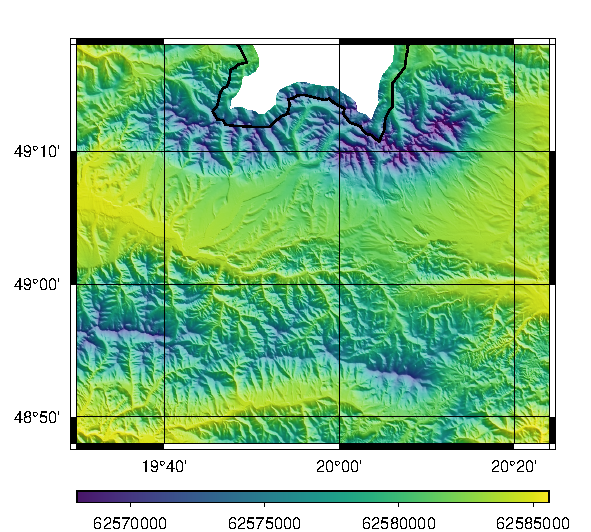
\includegraphics{./fig-vg-grav-sr-2arcsec.pdf}
\caption{Gravitačný potenciál~$V_\gidx$ na zemskom povrchu v~oblasti Vysokých
a~Nízkych Tatier (jednotky~$\mathrm{m}^2 \ \mathrm{s}^{-2}$).  Dáta sú prevzaté
z~modelu \texttt{grav-sr-2arcsec} \parencite{GravSR2arcsec}.}
\label{fig:vg_grav_sr_2arcsec}
\end{figure}

\subsubsection{Podmienka regularity}

Funkcia~$U$, ktorej súčiny
%
\begin{equation}
\label{eq:regular_function}
l \, U{,} \quad l^2 \, \frac{\partial U}{\partial x}{,} \quad l^2 \, 
\frac{\partial U}{\partial y}{,} \quad l^2 \, \frac{\partial U}{\partial z}
\end{equation}
%
nadobúdajú konečné hodnoty pre~$l \rightarrow \infty$, kde~$l$ je vzdialenosť 
od ľubovoľného pevného bodu, sa nazýva \emph{regulárna funkcia v~nekonečne} 
\parencite{Kellogg1967,Pick1973}.  Gravitačný potenciál~(\ref{eq:vg_body}) 
všeobecného telesa je regulárna funkcia v~nekonečne, pretože všetky štyri 
súčiny~(\ref{eq:regular_function}) nadobúdajú konečné hodnoty pre~$l 
\rightarrow \infty$.  V~tejto práci dokážeme toto tvrdenie iba pre limitu 
prvého súčinu,
%
\begin{equation}
\label{eq:vg_regular}
\lim_{l \rightarrow \infty} l \, V_\gidx = G \iiint\limits_{\tau} \rho \, 
\diff\tau = GM{,}
\end{equation}
%
kde~$M$ je hmotnosť všeobecného telesa.  Pre limity zvyšných troch súčinov 
pozri napríklad~\textcite{Pick1973}.






\section{Teória potenciálu}
\label{sec:potential_theory}

Rovnica~(\ref{eq:vg_body}) sa zvykne v~geovedách nazývať \emph{Newtonov
integrál}.  Hovorí, že ak poznáme tvar a~priestorové rozloženie hustoty telesa,
gravitačný potenciál telesa môže byť vypočítaný.  Newtonov
integrál má vo fyzikálnej geodézii kľúčový význam, nakoľko gravitačný potenciál 
obsahuje informáciu o~všetkých veličinách gravitačného poľa.

Newtonov integrál položil základy novej oblasti matematiky a~matematickej 
fyziky s~názvom \emph{teória potenciálu}.  Podľa \textcite{MacMillan1930} 
siahajú jej začiatky k~francúzskemu matematikovi, fyzikovi, astronómovi 
a~politikovi P.~S.~Laplaceovi (1749--1827).  Ten si uvedomil, že gravitačný 
potenciál každého všeobecného telesa má spoločné určité vlastnosti, čím vzniká 
zaujímavá množina funkcií hodná podrobnejšieho štúdia.  Významnosť teórie 
potenciálu iba potvrdzuje skutočnosť známa približne od čias C.~F.~Gaussa, 
a~síce že túto teóriu je možné aplikovať nielen na gravitačné pole, ale 
napríklad aj na magnetické či elektrostatické pole (spomeňme si na Coulombov 
zákon a~porovnajme ho s~Newtonovým gravitačným zákonom~\ref{eq:newton_law}).  
Teória potenciálu teda študuje vzťah~(\ref{eq:vg_body}) vo všeobecnom zmysle, 
zaoberá sa rozličnými zdrojmi poľa (hmotný bod, hmotná priamka, nekonečne tenká 
vrstva, všeobecné teleso a~pod.) s~rôznym priestorovým rozložením hustôt 
(konštantná, premenlivá, kladná, dokonca i~záporná a~pod.) a~neobmedzuje sa iba 
na gravitačné pole.  Táto úloha je nesmierne náročná.  Čo sa napríklad stane 
v~prípade, ak sa výpočtový bod~$P$ v~rovnici~(\ref{eq:vg_body}) nachádza vo 
vnútri telesa?  Za takýchto okolností musí nevyhnutne dôjsť k~situácii, 
v~ktorej sú súradnice bodu~$P$ identické so súradnicami jedného diferenciálneho 
hmotného elementu~$\diff m$.  Vzájomná vzdialenosť medzi bodom~$P$ 
a~elementom~$\diff m$, ktorá vystupuje v~menovateli, bude preto~$l = 0$.  
Konverguje alebo diverguje v~takejto situácii integrál~(\ref{eq:vg_body})?  
Jednou z~mnohých ďalších výziev sú gravitačné polia generované objektmi 
komplikovaných tvarov, napríklad Zemou, ktorej povrch obsahuje množstvo náhlych 
ostrých zmien.  Je preto prirodzené, že teória potenciálu pritiahla záujem 
brilantných matematikov akými boli, okrem iných, J.~L.~Lagrange, 
A.--M.~Legendre (1752~-- 1833), P.~S.~Laplace, britský samouk G.~Green 
(1793--1841) či C.~F.~Gauss (pre diskusiu o~Gaussovom prínose, pozri napríklad 
\cite{Freeden2018}).

V~nasledujúcich piatich kapitolách (\ref{sec:laplace_equation_cart}~--
\ref{sec:poisson_equation}) sa budeme zaoberať niektorými základnými
vlastnosťami gravitačného potenciálu, ktoré vyplývajú z~teórie potenciálu.
Vlastnosti budú popísané najprv pre gravitačný potenciál mimo telesa a~neskôr 
vo vnútri telesa.





\subsection{Laplaceova rovnica v~karteziánskych súradniciach}
\label{sec:laplace_equation_cart}

Pierre-Simon Laplace zistil, že gravitačný potenciál každého všeobecného telesa
spĺňa \emph{v~priestore mimo hmôt} rovnicu
%
\begin{equation}
\label{eq:vg_laplace_cart}
\nabla^2 V_\gidx = \Delta V_\gidx = \frac{\partial^2 V_\gidx}{\partial x^2}
+ \frac{\partial^2 V_\gidx}{\partial y^2} + \frac{\partial^2 V_\gidx}{\partial
z^2} = 0{.}
\end{equation}
%
Operátor~$\nabla^2 = \Delta$ sa nazýva \emph{Laplaceov operátor} 
a rovnica~(\ref{eq:vg_laplace_cart}) sa nazýva \emph{Laplaceova rovnica} pre
gravitačný potenciál.

Laplaceov operátor definujeme pomocou operátora gradient nasledovne
\parencite{SansoGeoidDetermination},
%
\begin{equation}
\label{eq:laplace_grad_grad_notation}
\nabla^2 = \nabla \cdot \nabla{,}
\end{equation}
%
kde symbol $\cdot$ označuje \emph{skalárny súčin dvoch vektorov}.  
Operátor~$\nabla^2$ v~trojrozmernom karteziánskom súradnicovom systéme získame 
pomocou vzťahov~(\ref{eq:laplace_grad_grad_notation}) a~(\ref{eq:gradient}),
%
\begin{equation}
\label{eq:laplace_xyz}
\begin{split}
\nabla^2 &= \nabla \cdot \nabla = \left( \vec e_1 \, \frac{\partial}{\partial 
x} + \vec e_2 \, \frac{\partial}{\partial y} + \vec e_3 \, 
\frac{\partial}{\partial z} \right) \cdot \left( \vec e_1 \, 
\frac{\partial}{\partial x} + \vec e_2 \, \frac{\partial}{\partial y} + \vec 
e_3 \, \frac{\partial}{\partial z} \right)\\
%
&=\vec e_1 \cdot \frac{\partial \vec e_1}{\partial x} \, 
\frac{\partial}{\partial x} + \vec e_1 \cdot \vec e_1 
\frac{\partial^2}{\partial x^2} + \vec e_1 \cdot \frac{\partial \vec 
e_2}{\partial x} \, \frac{\partial}{\partial y} + \vec e_1 \cdot \vec e_2 
\frac{\partial^2}{\partial x \, \partial y} + \dots + \vec e_3 \cdot \vec e_3 
\frac{\partial^2}{\partial z^2}\\
%
&=\frac{\partial^2}{\partial x^2} + \frac{\partial^2}{\partial y^2} 
+ \frac{\partial^2}{\partial z^2}{.}
\end{split}
\end{equation}
%
V~rovnici~(\ref{eq:laplace_xyz}) sme využili nasledovné vlastnosti 
jednotkových vektorov a~skalárneho súčinu dvoch vektorov,
%
\begin{align}
\label{eq:ei_orthogonality}
\vec e_i \cdot \vec e_j &= \| \vec e_i \| \, \| \vec e_j \| \, \cos(90^\circ) 
= 0{,} \quad i \neq j{,}\\
%
\label{eq:ei_unit_length}
\vec e_i \cdot \vec e_i &= \| \vec e_i \| \, \| \vec e_i \| \, \cos(0^\circ) 
= 1{,}\\
%
\label{eq:ei_derivatives}
\frac{\partial \vec e_i}{\partial x} &= \frac{\partial \vec e_i}{\partial y} 
= \frac{\partial \vec e_i}{\partial z} = \vec 0{.}
\end{align}
%
Rovnica~(\ref{eq:ei_orthogonality}) vyplýva z~\emph{ortogonálnosti} 
jednotkových vektorov~$\vec e_i$ a~$\vec e_j$ pre~$i \neq j$ (pozri 
Obrázok~\ref{fig:3d_coord_system}).  Rovnica~(\ref{eq:ei_unit_length}) je 
dôsledkom vzťahu~(\ref{eq:unit_vectors_unit_length}).  
Vzťahy~(\ref{eq:ei_derivatives}) vyplývajú z~definície jednotkových 
vektorov~(\ref{eq:unit_vectors}).

Laplaceov operátor je \emph{lineárny}, teda pre dvakrát diferencovateľné 
funkcie $f$ a~$g$ a~konštantu~$c$ platí
%
\begin{align}
\label{eq:laplace_additivity}
\nabla^2 \left(f + g \right) &= \nabla^2 f + \nabla^2 g{,}\\
%
\label{eq:laplace_homogenity}
\nabla^2 (c \, f) &= c \, \nabla^2 f{.}
\end{align}

Je dôležité upozorniť, že zápis $\nabla^2 = \nabla \cdot \nabla$ kombinovaný 
s~posledným výrazom rovnice~(\ref{eq:gradient}) môže poľahky viesť 
k~nesprávnemu vyjadreniu Laplaceovho operátora.  V~tomto nesprávnom prístupe sú 
vynásobené zodpovedajúce si prvky operátora gradient (pozri posledný výraz 
v~rovnici~\ref{eq:gradient}) a~následne sú získané súčiny sčítané (v~súlade 
s~definíciou skalárneho súčinu dvoch vektorov).  Hoci 
v~prípade~(\ref{eq:gradient}) získame správny tvar Laplaceovho operátora aj 
takýmto spôsobom, neskôr v~Prílohe~\ref{app:laplace_in_spherical_system} sa 
presvedčíme, že tento postup nie je vo všeobecnosti správny.  Dôvod je ten, že 
jednotkové vektory súradnicového systému môžu závisieť od premenných, podľa 
ktorých sa derivuje.  V~poslednom výraze rovnice~(\ref{eq:gradient}) však táto 
závislosť nie je explicitne uvedená.  Tejto chybe sa vyhneme, ak operátor 
gradient vyjadríme pomocou jednotkových vektorov (pozri predposledný výraz 
v~rovnici~\ref{eq:gradient}) a~tento tvar následne dosadíme 
do~(\ref{eq:laplace_grad_grad_notation}) (pozri rovnicu~\ref{eq:laplace_xyz}).  
Posledný výraz rovnice~(\ref{eq:gradient}) je preto potrebné vnímať 
predovšetkým formálne, pričom je vždy nutné mať na pamäti súradnicový systém, 
v~ktorom je operátor gradient vyjadrený.  V~mnohých situáciách je ale táto 
forma názorná a~zjednodušuje zápis, preto na miestach, kde by nemalo dôjsť 
k~nesprávnej interpretácii ju budeme používať.

Skúsme overiť, či gravitačný potenciál hmotného bodu~(\ref{eq:vg_point_mass}) 
vyhovuje Laplaceovej rovnici~(\ref{eq:vg_laplace_cart}).  Budeme uvažovať 
vzdialenosť~$l > 0$ nakoľko gravitačný potenciál hmotného bodu nie je 
definovaný pre~$l = 0$.  S~uvážením~(\ref{eq:laplace_homogenity}) postačuje 
dokázať rovnosť
%
\begin{equation}
\label{eq:nabla_l}
\nabla^2 \left( \frac{1}{l} \right) = 0{,}
\end{equation}
%
pretože~$G \, m$ je konštanta.  Vypočítajme preto druhé parciálne
derivácie funkcie~$1 \slash l$,
%
\begin{equation}
\label{eq:l_2nd_derivatives}
\begin{split}
\frac{\partial^2}{\partial x^2} \left( \frac{1}{l} \right) &=
-\frac{\partial}{\partial x} \left( \frac{x - x_Q}{l^3} \right) = \left(3
\frac{(x - x_Q)^2}{l^5} - \frac{1}{l^3} \right){,}\\
%
\frac{\partial^2}{\partial y^2} \left( \frac{1}{l} \right) &=
-\frac{\partial}{\partial y} \left( \frac{y - y_Q}{l^3} \right) = \left(3
\frac{(y - y_Q)^2}{l^5} - \frac{1}{l^3} \right){,}\\
%
\frac{\partial^2}{\partial z^2} \left( \frac{1}{l} \right) &=
-\frac{\partial}{\partial z} \left( \frac{z - z_Q}{l^3} \right) = \left(3
\frac{(z - z_Q)^2}{l^5} - \frac{1}{l^3} \right){.}
\end{split}
\end{equation}
%
Súčet členov na pravej strane predošlých troch rovníc je nulový, čím bolo
dokázané, že gravitačný potenciál hmotného bodu vyhovuje Laplaceovej
diferenciálnej rovnici~(\ref{eq:vg_laplace_cart}) pre~$l > 0$.

Využitím vzťahov~(\ref{eq:l_2nd_derivatives}) a~vlastností Laplaceovho
operátora~(\ref{eq:laplace_additivity}) a~(\ref{eq:laplace_homogenity}) je
možné presvedčiť sa, že Laplaceovej rovnici vyhovuje i~gravitačný potenciál
generovaný sústavou~$N$ hmotných bodov,
%
\begin{equation}
\nabla^2 \left( \sum_{i = 1}^N V_{\gidx,i} \right) = \sum_{i = 1}^N \nabla^2
V_{\gidx,i} = 0{,}
\end{equation}
%
ako aj gravitačný potenciál všeobecného telesa v~bode \emph{mimo telesa},
%
\begin{equation}
\nabla^2 V_\gidx = G\, \iiint\limits_\tau \rho \, \left[ 
\frac{\partial^2}{\partial
x^2}\left(\frac{1}{l}\right) + \frac{\partial^2}{\partial
y^2}\left(\frac{1}{l}\right) + \frac{\partial^2}{\partial
z^2}\left(\frac{1}{l}\right) \right] \diff\tau = 0{.}
\end{equation}


\subsection{Laplaceova rovnica vo sférických súradniciach}
\label{sec:laplace_equation_sph}

Kvôli približne sférickému tvaru Zeme je často výhodnejšie popisovať zemské 
gravitačné pole v~krivočiarych sférických súradniciach než v~karteziánskych 
súradniciach.  Je preto potrebné nájsť tvar operátora gradient 
(rovnica~\ref{eq:gradient}) a~Laplaceovho operátora 
(rovnica~\ref{eq:vg_laplace_cart}) aj vo sférických súradniciach.  
Zaujímavosťou je, že Laplace v~skutočnosti prvýkrát publikoval 
rovnicu~(\ref{eq:vg_laplace_cart}) práve v~krivočiarych sférických 
súradniciach, a~nie v~karteziánskych súradniciach \parencite{MacMillan1930}.

Sférické súradnice budeme označovať symbolmi~$r$, $\varphi$ a $\lambda$, 
pričom~$r$ predstavuje sprievodič, $\varphi$ je sférická šírka a~$\lambda$ je 
sférická dĺžka (Obrázok~\ref{fig:cart_sph}).  Medzi sférickými a~karteziánskym 
súradnicami platia vzťahy (pozri Obrázok~\ref{fig:cart_sph})
%
\begin{equation}
\label{eq:sph2cart}
\begin{split}
x &= r \, \cos\varphi \, \cos\lambda{,}\\
y &= r \, \cos\varphi \, \sin\lambda{,}\\
z &= r \, \sin\varphi\\
\end{split}
\end{equation}
%
a
%
\begin{equation}
\label{eq:cart2sph}
\begin{split}
r &= \sqrt{x^2 + y^2 + z^2}{,}\\
\varphi &= \arctan \frac{z}{\sqrt{x^2 + y^2}}{,}\\
\lambda &= \arctan \frac{y}{x}{.}\\
\end{split}
\end{equation}

\begin{figure}
\centering
\input{./fig-cart-sph.pdf_tex}
\caption{Karteziánske súradnice~$x$, $y$, $z$ a~sférické súradnice~$r$, 
$\varphi$, $\lambda$ bodu~$P$.  Symboly~$\vec{e}_1^\mathrm{s}$, 
$\vec{e}_2^\mathrm{s}$ a~$\vec{e}_3^\mathrm{s}$ označujú jednotkové vektory 
lokálneho karteziánskeho súradnicového systému~$x^\mathrm{s}$, $y^\mathrm{s}$, 
$z^\mathrm{s}$ s~pohyblivým začiatkom v~bode~$P$.}
\label{fig:cart_sph}
\end{figure}

Operátor gradient má vo sférických súradniciach tvar (pozri 
Prílohu~\ref{app:gradient_in_orthogonal_systems})
%
\begin{equation}
\label{eq:gradient_sph}
\nabla = \grad = \vec e_1^\mathrm{s} \, \frac{1}{r} \, \frac{\partial}{\partial 
\varphi} + \vec e_2^\mathrm{s} \, \frac{1}{r \, \cos\varphi} \, 
\frac{\partial}{\partial \lambda} + \vec e_3^\mathrm{s} 
\frac{\partial}{\partial r}\\
%
=
%
\begin{bmatrix}
\dfrac{1}{r} \, \dfrac{\partial}{\partial \varphi} \\[2ex]
\dfrac{1}{r \, \cos\varphi} \, \dfrac{\partial}{\partial \lambda}\\[2ex]
\dfrac{\partial}{\partial r}
\end{bmatrix}
{.}
\end{equation}
%
Symboly~$\vec{e}_1^\mathrm{s}$, $\vec{e}_2^{\mathrm{s}}$, 
$\vec{e}_3^\mathrm{s}$ označujú jednotkové vektory súradnicových 
osí~$x^\mathrm{s}$, $y^\mathrm{s}$, $z^\mathrm{s}$ lokálneho karteziánskeho 
súradnicového systému orientovaného na sever s~pohyblivým začiatkom 
v~bode~$P$~(Obrázok~\ref{fig:cart_sph}).  Os~$z^\mathrm{s}$ je daná smerom 
sprievodiča prechádzajúceho bodom~$P$ a~je orientovaná kladne vo vonkajšom 
smere.  Os~$x^\mathrm{s}$ leží v~rovine meridiánu a~je orientovaná kladne na 
sever.  Os~$y^\mathrm{s}$ dotvára pravouhlý \emph{ľavotočivý} súradnicový 
systém.  Aplikovaním operátora gradient~(\ref{eq:gradient_sph}) na gravitačný 
potenciál~$V_\gidx(r, \varphi, \lambda)$ získame vektor gravitačného 
zrýchlenia~$\vec g_\gidx(r, \varphi, \lambda)$, ktorého prvky popisujú zmenu 
gravitačného potenciálu v~bode~$P$ v~smere súradnicových osí~$x^\mathrm{s}$, 
$y^\mathrm{s}$ a~$z^\mathrm{s}$.

Laplaceova rovnica pre gravitačný potenciál má vo sférických súradniciach tvar 
(Príloha~\ref{app:laplace_in_spherical_coordinates})
%
\begin{equation}
\label{eq:vg_laplace_sph}
\nabla^2 V_\gidx = \frac{1}{r^2} \frac{\partial}{\partial r} \left( r^2
\frac{\partial V_\gidx}{\partial r} \right) + \frac{1}{r^2 \, \cos\varphi}
\frac{\partial}{\partial \varphi} \left( \cos\varphi \frac{\partial
V_\gidx}{\partial \varphi} \right) + \frac{1}{r^2 \,
\cos^2\varphi}\frac{\partial^2 V_\gidx}{\partial \lambda^2} = 0{.}
\end{equation}


\subsection{Praktický význam Laplaceovej rovnice}
\label{sec:meaning_of_laplace_equation_in_practice}

Jedným z~cieľov fyzikálnej geodézie je určiť vonkajšie gravitačné pole Zeme 
z odmeraných veličín gravitačného poľa.  Z~praktických dôvodov je ale možné 
vykonávať merania iba v~malej časti priestoru mimo Zeme, napríklad 
v~bezprostrednej blízkosti zemského povrchu či na dráhe umelej družice Zeme.  
Preto ak chceme určiť gravitačné pole v~celom priestore mimo Zeme, bolo by 
vhodné porozumieť tomu, ako sa gravitačný potenciál v~priestore mení.  Ak by 
nejaký princíp existoval a~bol by objavený, znamenalo by to, že hoci naše 
merania sú dostupné iba v~malej časti vonkajšieho priestoru Zeme, dokázali by 
sme predikovať gravitačný potenciál kdekoľvek mimo Zeme, teda aj v~oblastiach 
bez dostupných meraní.

Tento princíp bol objavený a~je ním práve Laplaceova rovnica.  
V~Kapitole~\ref{sec:newton_law} sme ukázali, ako Newtonov gravitačný 
zákon~(\ref{eq:newton_law}) vysvetľuje \emph{princíp} (mechanizmus) pohybu 
planéty okolo Slnka.  Vďaka tomuto princípu postačuje poznať niekoľko vstupných 
údajov v~čase~$t_0$ (polohy planéty a~Slnka, ich rýchlosti a~pôsobiace 
gravitačné sily) a~poloha planéty môže byť vypočítaná v~ľubovoľnom čase 
v~budúcnosti či v~minulosti.  Úloha je síce výrazne komplikovanejšia, ak 
uvážime prítomnosť ďalších nebeských telies, pretože aj tie ovplyvňujú svojou 
gravitačnou silou našu planétu a~naša planéta ovplyvňuje svojou gravitačnou 
silou ostatné planéty, no úloha je riešiteľná rovnakým spôsobom.  V~prípade 
Laplaceovej rovnice je situácia veľmi podobná.  Ak poznáme napríklad gravitačný 
potenciál či gravitačné zrýchlenie na celom povrchu Zeme, znalosť 
\emph{princípu} zmeny gravitačného potenciálu\footnote{Presnejšie by azda bolo 
povedať \textit{zmenu zmeny} gravitačného potenciálu, keďže Laplaceova 
rovnica~(\ref{eq:vg_laplace_cart}) obsahuje druhé derivácie.} mimo Zeme 
v~podobe Laplaceovej rovnice umožňuje zistiť, akú hodnotu nadobúda gravitačný 
potenciál v~ľubovoľnom bode tejto oblasti.  Laplaceova rovnica má preto kľúčový 
význam v~procese určovania vonkajšieho gravitačného poľa Zeme.




\subsection{Harmonická funkcia}
\label{sec:harmonic_function}

Laplaceovej rovnici vyhovuje nielen gravitačný potenciál mimo telesa, ale
nekonečné množstvo funkcií.  Zaveďme preto pojem \emph{harmonická funkcia}.
Harmonická funkcia je taká funkcia, ktorá má spojité prvé a~druhé parciálne
derivácie na otvorenej množine~$\Omega$ a~vyhovuje Laplaceovej rovnici
%
\begin{equation}
\nabla^2 f = 0
\end{equation}
%
v~každom bode oblasti~$\Omega$.

Každá harmonická funkcia je \emph{analytická} v~oblasti, v~ktorej vyhovuje
Laplaceovej rovnici \parencite{MoritzPhysicalGeodesy}.  To znamená, že každá
harmonická funkcia je spojitá, má spojité všetky derivácie a~v každom bode
oblasti~$\Omega$ ju možno rozvinúť do mocninového radu (napríklad Taylorovho),
ktorý konverguje.  Táto vlastnosť je dôležitá, preto sa pri nej na chvíľku
pristavme.

Uvažujme všeobecné teleso generujúce gravitačné pole.  Nech sú dané dva body,
$P_1(r, \varphi, \lambda)$ a~$P_2(r + \Delta r, \varphi, \lambda)$, $\Delta
r > 0$, nachádzajúce sa mimo tohto telesa a~na tej istej spojnici so začiatkom
súradnicového systému, ktorý sa nachádza v~ťažisku telesa
(Obrázok~\ref{fig:analytical_continuation}).  Keďže gravitačný potenciál mimo
telesa je harmonická, a~teda analytická, funkcia, môžeme ho v~bode~$P_1$
rozvinúť do Taylorovho radu, ktorý konverguje,
%
\begin{equation}
\label{eq:vg_analytical_continuation}
V_\gidx(P_2) = \sum_{i = 0}^\infty \frac{1}{i!} \, \left.\frac{\partial^i
V_\gidx}{\partial r^i}\right|_{P_1} \, \Delta r^i{.}
\end{equation}
%
Symbol $\left.\frac{\partial^i V_\gidx}{\partial r^i} \right|_{P_1}$ označuje 
$i$-tu deriváciu gravitačného potenciálu~$V_\gidx$ v~bode~$P_1$.

\begin{figure}

\centering
\input{./fig-analytical-continuation.pdf_tex}
\caption{Analytické pokračovanie gravitačného poľa z~bodu~$P_1$ do bodu~$P_2$.}
\label{fig:analytical_continuation}
\end{figure}

Rovnica~(\ref{eq:vg_analytical_continuation}) hovorí, že z~lokálnych vlastností 
gravitačného potenciálu, ktoré sú obsiahnuté v~deriváciách~$\partial^i V_\gidx 
\slash \partial r^i$ v~bode~$P_1$, dokážeme určiť hodnotu gravitačného 
potenciálu v~ľubovoľnom bode v~radiálnom smere pre~$\Delta r > 0$.  Tento 
proces sa nazýva \emph{analytické pokračovanie} gravitačného potenciálu nahor.  
Čím je väčšia vzdialenosť~$\Delta r$, tým pomalšie 
rad~(\ref{eq:vg_analytical_continuation}) konverguje a~naopak.  Analyticky 
pokračovať je možné aj v~iných smeroch ako v~radiálnom.  V~takom prípade je 
potrebné derivovať gravitačný potenciál v~príslušnom smere.  Rovnako tak je 
možné analyticky pokračovať aj iné veličiny gravitačného poľa, napríklad vektor 
gravitačného zrýchlenia,
%
\begin{equation}
\label{eq:gg_analytical_continuation}
\vec g_\gidx(P_2) = \sum_{i = 0}^{\infty} \frac{1}{i!} \, 
\left.\frac{\partial^i \vec
g_\gidx}{\partial r^i}\right|_{P_1} \, \Delta r^i{.}
\end{equation}

Na záver dodajme, že situácia je výrazne komplikovanejšia, ak analyticky 
pokračujeme nadol z~bodu~$P_2$ do bodu~$P_1$.  Táto úloha je zle podmienená 
a numericky nestabilná \parencite{SansoGeodeticBoundaryValueProblem}.  
V~praktických aplikáciách to znamená, že i~malá chyba vo vstupných dátach 
spôsobuje veľké chyby vo výsledkoch.






\subsection{Poissonova rovnica}
\label{sec:poisson_equation}

Z~Kapitoly~\ref{sec:laplace_equation_cart} vieme, že Laplaceova rovnica pre
gravitačný potenciál platí v~každom bode mimo telesa.  \emph{Vo vnútri} telesa
platí \emph{Poissonova rovnica},
%
\begin{equation}
\label{eq:vg_poisson_equation}
\nabla^2 V_\gidx(P) = -4 \pi \, G \, \rho(P){,}
\end{equation}
%
kde~$\rho(P)$ je hustota v~bode~$P$.  Odvodenie Poissonovej rovnice je možné 
nájsť napríklad v~\textcite{MacMillan1930}, \textcite{Kellogg1967} či 
\textcite{SansoGeoidDetermination}.  Poissonovu rovnicu je možné vnímať ako 
zovšeobecnenie Laplaceovej rovnice.  Ak sa bod~$P$ vo 
vzťahu~(\ref{eq:vg_poisson_equation}) nachádza mimo hmôt, potom~$\rho(P) = 0$, 
čím dostávame Laplaceovu rovnicu~(\ref{eq:vg_laplace_cart}).  S.~D.~Poisson 
(1781~-- 1840) bol francúzsky matematik a~fyzik.  
Rovnicu~(\ref{eq:vg_poisson_equation}) publikoval v~roku 1813 v~práci 
\textit{Bulletin de la société philomatique}.

Posledná oblasť, v~ktorej sa môže nachádzať bod~$P$, no nie je pokrytá ani 
Laplaceovou, ani Poissonovou rovnicou, je \emph{povrch} telesa.  Druhé 
derivácie gravitačného potenciálu vystupujúce v~operátore $\nabla^2$ (pozri 
rovnice~\ref{eq:vg_laplace_cart} a~\ref{eq:vg_laplace_sph}) nie sú vo 
všeobecnosti v~takom prípade definované \parencite{Kellogg1967}.  Dôvodom je 
nespojitosť hustoty~$\rho$, ktorá sa na povrchu mení z~$\rho \neq 0$ na 0, 
resp. naopak, v~závislosti od smeru prechodu.






\section{Odstredivé pole a~tiažové pole}
\label{sec:centrifugal_gravity_field}

Newtonov gravitačný zákon~(\ref{eq:newton_law}) platí v~súradnicovom systéme,
ktorý je v~pokoji alebo je v~stave rovnomerného priamočiareho pohybu.  Takýto
súradnicový systém sa nazýva \emph{inerciálny súradnicový systém}.

Uvažujme trojrozmerný karteziánsky súradnicový systém so začiatkom v~ťažisku 
Zeme a~s~osou~$z$, ktorá je totožná s~rotačnou osou Zeme.  Nech tento 
súradnicový systém rotuje spolu so Zemou uhlovou rýchlosťou~$\omega$.  Takýto 
súradnicový systém nie je inerciálny, pretože vzhľadom na inerciálny 
súradnicový systém v~ňom dochádza prinajmenšom k~dvom nelineárnym pohybom.  
Prvý vzniká v~dôsledku rotácie Zeme okolo vlastnej osi, druhý je spôsobený 
obehom Zeme okolo Slnka.  Ak chceme študovať sily pôsobiace na Zemi v~takomto 
neinerciálnom súradnicovom systéme, potrebné je uvážiť nielen gravitačnú silu, 
ale aj~ďalšie sily v~zmysle Newtonovho pohybového zákona.  Na objekt, ktorý sa 
nachádza na rotujúcej Zemi a~je vzhľadom k~nej v~pokoji, pôsobí okrem 
gravitačnej sily aj \emph{odstredivá sila}.  Ak je objekt v~pohybe, pôsobí naň 
aj \emph{Coriolisova sila} 
\parencite{Torge1989,Jekeli2000,SansoGeoidDetermination}.  Azda väčšina 
geodetických meracích zariadení je počas merania vzhľadom k~Zemi v~pokoji, 
preto Coriolisovu silu nebudeme ďalej uvažovať.  Na záver 
spomeňme~\emph{Eulerovu silu}, ktorá je spôsobená zmenou uhlovej rýchlosti 
rotácie~$\omega$ v~čase \parencite{Torge1989,SansoGeoidDetermination}.  V~tejto 
práci predpokladáme, že uhlová rýchlosť rotácie Zeme je konštantná, preto 
nebudeme ďalej uvažovať ani Eulerovu silu.  Tieto tri sily, odstredivá, 
Coriolisova a~Eulerova, sa zaraďujú medzi \emph{zotrvačné sily}, niekedy tiež 
nazývané fiktívne sily.  Zotrvačné sily sú zdanlivé sily, ktoré sú spôsobené 
neinerciálnosťou vzťažnej sústavy pozorovateľa, a~teda nevznikajú vzájomným 
silovým pôsobením medzi objektmi.






\subsection{Odstredivé a~tiažové zrýchlenie}
\label{sec:centrifugal_and_gravity_acceleration}

Najvýznamnejšia zotrvačná sila vo fyzikálnej geodézii je \emph{odstredivá sila}
$\vec F_\cidx$.  Uvažujme neinerciálny súradnicový systém v~zmysle predošlého
odseku a~hmotný bod~$P(x, y, z)$ s~hmotnosťou~$1\ \mathrm{kg}$.  V~dôsledku
nelineárnych pohybov súradnicového systému je tomuto hmotnému bodu udeľované
\emph{odstredivé zrýchlenie}~$\vec g_\cidx(P)$,
%
\begin{equation}
\label{eq:gc}
\vec g_\cidx(P) = \omega^2 \, \vec p =
%
\omega^2 \, \begin{bmatrix}
x\\
y\\
0
\end{bmatrix}
{.}
\end{equation}
%
Za predpokladu konštantnej uhlovej rýchlosti rotácie~$\omega$ sa veľkosť
odstredivého zrýchlenia mení iba so vzdialenosťou~$p = \| \vec p \|$ od 
rotačnej osi (Obrázok~\ref{fig:gravity_vector}),
%
\begin{equation}
\| \vec g_\cidx \| = \omega^2 \, p = \omega^2 \, \sqrt{x^2 + y^2}{.}
\end{equation}
%
Čím je vzdialenosť~$p$ väčšia, tým je väčšie i~odstredivé zrýchlenie a~naopak.
Zo vzťahu~(\ref{eq:gc}) je zrejmé, že odstredivé zrýchlenie je kolmé na os
rotácie a~má smer vzďaľujúci sa od rotačnej osi
(Obrázok~\ref{fig:gravity_vector}).  Uhlová rýchlosť rotácie Zeme je približne
rovná~$\omega = 7\, 292\, 115 \times 10^{-11} \ \mathrm{rad} \ \mathrm{s}^{-1}$ 
\parencite{GRS80}{.}

\begin{figure}
\centering
\input{./fig-gravity-vector.pdf_tex}
\caption{Vektory gravitačného~$\vec g_\gidx$, odstredivého~$\vec g_\cidx$
a~tiažového zrýchlenia~$\vec g$ v~bode~$P$ na povrchu idealizovanej rotujúcej
Zeme sférického tvaru a~konštantnej hustoty.}
\label{fig:gravity_vector}
\end{figure}

Výsledné zrýchlenie pôsobiace na hmotný bod s~hmotnosťou~$1 \ \mathrm{kg}$ je
v~neinerciálnom systéme dané súčtom gravitačného zrýchlenia~$\vec g_\gidx(P)$
a~odstredivého zrýchlenia~$\vec g_\cidx(P)$.\footnote{Ostatné zrýchlenia (pozri
Kapitolu~\ref{sec:centrifugal_gravity_field}) sme pre účely tejto práce 
s~prijateľnou mierou aproximácie zanedbali.}  Toto zrýchlenie sa nazýva 
\emph{tiažové zrýchlenie} a~budeme ho označovať symbolom~$\vec g(P)$ 
(Obrázok~\ref{fig:gravity_vector}),
%
\begin{equation}
\label{eq:g}
\vec g(P) = \vec g_\gidx(P) + \vec g_\cidx(P){.}
\end{equation}


\subsubsection{Meranie tiažového zrýchlenia}
\label{sec:gravity_measurements}

Vektor tiažového zrýchlenia je možné odmerať, a~tak predstavuje ústrednú 
veličinu v~procese určovania tvaru Zeme.  Prístroj na meranie \emph{veľkosti} 
vektora tiažového zrýchlenia~$\| \vec g(P) \|$ sa nazýva \emph{absolútny 
gravimeter}.  Merania absolútnymi gravimetrami sú časovo aj finančne náročné, 
preto sa využívajú aj \emph{relatívne gravimetre}.  Týmito prístrojmi je ale 
možné určiť iba rozdiel veľkostí tiažového zrýchlenia, či už medzi dvoma bodmi 
alebo na jednom bode, no v~inom čase.  V~súčasnosti bežná presnosť určenia~$\| 
\vec g(P) \|$ dosahuje hodnotu niekoľkých mikroGalov.  \emph{Smer} vektora 
tiažového zrýchlenia je možné odmerať astronomickým určením zemepisnej šírky 
a~zemepisnej dĺžky bodu~$P$.  Presnosť určenia astronomických súradníc sa 
v~súčasnosti pohybuje približne v~desatinách uhlovej sekundy.    Vedný odbor 
zaoberajúci sa meraním tiažového zrýchlenia sa nazýva \emph{gravimetria} (pozri 
napríklad \cite{Torge1989,Rozimant1994} či \cite{Janak2010}).  






\subsection{Odstredivý a~tiažový potenciál}
\label{sec:centrifugal_and_gravity_potential}

Podobne ako gravitačné zrýchlenie, i~odstredivé a~tiažové zrýchlenie je
možné definovať pomocou skalárnych veličín.  Tieto skalárne veličiny sa
nazývajú \emph{odstredivý potenciál},
%
\begin{equation}
\label{eq:vc}
V_c(P) = \frac{1}{2} \, \omega^2 \, (x^2 + y^2){,}
\end{equation}
%
a~\emph{tiažový potenciál},
%
\begin{equation}
\label{eq:w}
W(P) = V_\gidx(P) + V_\cidx(P){.}
\end{equation}
%
Príslušné zrýchlenia~(\ref{eq:gc}) a~(\ref{eq:g}) získame aplikovaním operátora
gradient na tieto rovnice,
%
\begin{equation}
\label{eq:gc_vc}
\vec g_\cidx(P) = \nabla V_c(P)
\end{equation}
%
a
%
\begin{equation}
\label{eq:g_gradW}
\vec g(P) = \nabla W(P) = \nabla V_\gidx(P) + \nabla V_\cidx(P) = \vec
g_\gidx(P) + \vec g_\cidx(P){.}
\end{equation}
%
Vektory~$\vec g_\cidx(P)$ a~$\vec g(P)$ udávajú v~zmysle vlastností operátora 
gradient (Kapitola~\ref{sec:vg}) veľkosť a~smer najväčšieho nárastu
odstredivého a~tiažového potenciálu~$V_\cidx(P)$ a~$W(P)$ v~bode~$P$.  Platnosť
rovnice~(\ref{eq:gc_vc}) možno overiť pomocou~(\ref{eq:gradient})
a~(\ref{eq:vc}), čím získame~(\ref{eq:gc}).  V~rovnici~(\ref{eq:g_gradW}) bola
využitá lineárnosť operátora gradient (rovnice~\ref{eq:gradient_additivity} 
a~\ref{eq:gradient_homogenity}).

Odstredivý ani tiažový potenciál nedokážeme priamo odmerať.  V~sústave SI 
prislúcha obom veličinám jednotka~$\mathrm{m}^2 \ \mathrm{s}^{-2}$.

\subsubsection{Ekvipotenciálna plocha}
\label{sec:equipotential_surface}

Plocha, na ktorej je tiažový potenciál~$W$ konštantný, sa nazýva 
\emph{ekvipotenciálna plocha} (Obrázok~\ref{fig:equipotential_surfaces}).  
V~úvodnej kapitole jeden z~prístupov definuje tvar Zeme ako geoid, teda tú 
ekvipotenciálnu plochu, ktorá sa najlepšie približuje strednej hladine morí 
a~oceánov.  Pre fyzikálnu geodéziu majú preto ekvipotenciálne plochy veľký 
význam.  Zamerajme sa na niektoré ich vlastnosti.

\begin{figure}
\centering
\input{./fig-equipotential-surfaces.pdf_tex}
\caption{Ekvipotenciálne plochy s~konštantným krokom tiažového 
potenciálu~$\delta W$.}
\label{fig:equipotential_surfaces}
\end{figure}

\begin{itemize}
\item Ekvipotenciálne plochy sú spojité.  Táto vlastnosť vyplýva zo
skutočnosti, že tiažový potenciál všeobecného telesa~(rovnica~\ref{eq:w}) je 
spojitá funkcia v~celom priestore \parencite{MoritzPhysicalGeodesy}.

\item Ekvipotenciálne plochy sú uzavreté \parencite{VanicekGeodesy}.

\item Ak sa celá ekvipotenciálna plocha nachádza mimo telesa, potom je táto 
plocha analytická.  Ekvipotenciálne plochy nachádzajúce sa vo vnútri telesa 
alebo teleso pretínajúce nie sú analytické, pretože ich krivosť sa môže 
nespojito meniť v~závislosti od hustoty \parencite{MoritzPhysicalGeodesy}.

\item Všetky ekvipotenciálne plochy sú hladké a~neobsahujú hrany
\parencite{MoritzPhysicalGeodesy}.

\item Ekvipotenciálne plochy sa nepretínajú.  Tiažový potenciál~$W$ má v~každom 
bode definované práve jednu hodnotu (skalárna veličina), preto sa 
ekvipotenciálne plochy nemôžu pretnúť \parencite{MacMillan1930}.

\item Vektor tiažového zrýchlenia v~ľubovoľnom bode je kolmý na ekvipotenciálnu
plochu prechádzajúcu týmto bodom \parencite{MoritzPhysicalGeodesy}.  Toto 
tvrdenie vyplýva priamo z~rovnice~(\ref{eq:g_gradW}).
\end{itemize}

Matematický popis tvaru ekvipotenciálnych plôch reálnych telies je náročný.  
Z~Newtonovho integrálu~(\ref{eq:vg_body}) vieme (pozri tiež 
Kapitolu~\ref{sec:potential_theory}), že gravitačné pole je dané tvarom 
a hustotou telesa.  Zložité nepravidelné tvary či rozloženia hustoty spôsobujú 
zvlnenia ekvipotenciálnych plôch.  Na regionálnej úrovni je nepravidelný tvar 
ekvipotenciálnych plôch do veľkej miery spôsobený lokálnymi hmotami, napríklad 
pohoriami.  Z~globálneho pohľadu je tvar ekvipotenciálnych plôch daný skôr 
celkovou geometriou telesa (napríklad sploštenie Zeme) či rozsiahlymi 
hustotnými zmenami v~jeho vnútri.  Práve tieto skutočnosti výrazne komplikujú 
presný výpočet geoidu.  Podrobnejší popis niektorých dôležitých vlastností 
ekvipotenciálnych plôch, napríklad ich krivostí, je možné nájsť napríklad 
v~prácach \textcite{MoritzPhysicalGeodesy} a~\textcite{Janak2006}.

Obrázok~\ref{fig:equipotential_surfaces} schematicky znázorňuje ekvipotenciálne
plochy tiažového poľa Zeme s~konštantným krokom tiažového potenciálu~$\delta
W$.  Možno si všimnúť, že priestorový rozostup ekvipotenciálnych plôch je väčší
v~rovníkových oblastiach ako v~polárnych oblastiach.  Malý rozostup
ekvipotenciálnych plôch znamená veľkú zmenu tiažového poľa a~naopak.  Veľkosť
vektora tiažového zrýchlenia~$\| \vec g \|$ je tak väčšia v~oblasti pólov ako
v~oblasti rovníka.

Horizontovaním geodetického prístroja zabezpečujeme, že jeho horizontálna 
rovina (lokálny horizont) je dotyková k~ekvipotenciálnej ploche, ktorá 
prechádza stredom libely.  Z~dôvodu približne sférického tvaru Zeme a~zvlnenia 
ekvipotenciálnych plôch nemožno vo všeobecnosti predpokladať rovnobežnosť 
horizontálnych rovín na dvoch rôznych stanoviskách.  V~prípade teodolitu sú 
v~tejto rovine merané vodorovné smery.  Preto ak je vyžadovaná presnosť vysoká 
alebo záujmová lokalita je rozsiahla a~má zložitú topografiu,  merania je 
potrebné korigovať o~vplyv nerovnobežnosti horizontálnych rovín medzi 
stanoviskami \parencite[pozri napríklad][]{VanicekGeodesy}.

\subsubsection{Tiažnica}
\label{sec:plumbline}

Siločiara tiažového poľa sa nazýva \emph{tiažnica}.  Tiažnica je priestorová 
krivka, ktorá je kolmá na všetky ekvipotenciálne plochy 
(Obrázok~\ref{fig:equipotential_surfaces}).  Dotyčnica k~tiažnici sa nazýva 
\emph{zvislica}.  Smer zvislice je totožný so smerom vektora tiažového 
zrýchlenia, a~teda so smerom zavesenej olovnice.  V~geodézii sa tiažnice 
využívajú napríklad na definovanie fyzikálnych (nadmorských) výšok.  Jedna taká 
výška má názov \emph{ortometrická výška} a~je meraná pozdĺž tiažnice od geoidu 
po bod~$P$ (pozri Obrázok~\ref{fig:equipotential_surfaces}).

Z~pohľadu geodetických meraní je nutné, aby zvislá os prístroja (napríklad 
teodolitu) bola totožná s~lokálnou zvislicou.  Táto podmienka je splnená po 
zhorizontovaní prístroja za predpokladu, že horizontálna os prístroja je kolmá 
na vertikálnu os prístroja.  K~lokálnej zvislici sa vzťahujú napríklad merané 
vertikálne smery.  Približne sférický tvar Zeme a~zvlnenie ekvipotenciálnych 
plôch spôsobujú, že vertikálne osi zhorizontovaných prístrojov nie sú vo 
všeobecnosti rovnobežné medzi stanoviskami.  Podobne ako pri vodorovných 
smeroch, presné merania si môžu vyžadovať zavedenie korekcií.

\subsubsection{Určenie rozdielu tiažového potenciálu}
\label{sec:potential_differences}

Hoci tiažový potenciál priamo odmerať nedokážeme, \emph{rozdiel} tiažového 
potenciálu dokážeme určiť nepriamo kombináciou nivelácie a~gravimetrie.  Pred 
popísaním tejto metódy je ale potrebné pristaviť sa pri pojme totálny 
diferenciál.

Ak sa poloha bodu~$P$ zmení o~vektor~$\Delta \vec x$,
%
\begin{equation}
\label{eq:deltax}
\Delta \vec x =
\begin{bmatrix}
\Delta x\\
\Delta y\\
\Delta z
\end{bmatrix}
{,}
\end{equation}
%
potom tiažový potenciál~$W(P)$ sa zmení o~hodnotu~$\delta W(P, \Delta \vec x)$.  
\emph{Totálny diferenciál}~$\diff W(P, \diff \vec x)$ aproximuje skutočnú zmenu 
tiažového potenciálu~$\delta W(P, \Delta \vec x)$ vzťahom
%
\begin{equation}
\label{eq:w_totdiff_scalar}
\begin{split}
\delta W(P, \Delta \vec x) \approx \diff W(P, \diff \vec x) &= 
\left.\frac{\partial W}{\partial x}\right|_P \, \diff x + \, 
\left.\frac{\partial W}{\partial y}\right|_P \, \diff y + \left.\frac{\partial 
W}{\partial z}\right|_P \, \diff z\\
%
&= \nabla W(P) \cdot \diff \vec x = \vec g(P) \cdot \diff \vec x = \| \vec g(P) 
\| \, \| \diff \vec x \| \, \cos\alpha{,}
\end{split}
\end{equation}
%
kde
%
\begin{equation}
\label{eq:diffx}
\diff \vec x =
\begin{bmatrix}
\diff x\\
\diff y\\
\diff z
\end{bmatrix}
\end{equation}
%
a~$\alpha$ je uhol medzi vektormi~$\vec g(P)$ a~$\diff \vec x$.  Skracovaním 
vzdialenosti~$\diff \vec x$ v~rovnici~(\ref{eq:w_totdiff_scalar}) je možné 
zmenšiť aproximačnú chybu totálneho diferenciálu~$\diff W(P, \diff \vec x)$ 
voči skutočnej zmene tiažového potenciálu~$\delta W(P, \Delta \vec x)$ na 
ľubovoľne malú hodnotu.  Vo všeobecnosti môžeme povedať, že totálny diferenciál 
(diferencovateľnej) funkcie~$f$ v~bode~$P$ je najlepšia lineárna aproximácia 
funkcie~$f$ v~okolí bodu~$P$.

Ak k~diferenciálnej zmene polohy~$\diff \vec x$ dochádza pozdĺž 
ekvipotenciálnej plochy, potom totálny diferenciál~$\diff W$ je nulový (pozri 
vektory~$\diff \vec x_2$ a~$\diff \vec x_4$ na 
Obrázku~\ref{fig:total_differential}).  Toto tvrdenie môžeme vysvetliť tým, že 
vektor~$\vec g$ je kolmý na ekvipotenciálnu plochu (a~tým aj na vektor~$\diff 
\vec x$), preto $\diff W = \| \vec g \| \, \| \diff \vec x \| \, 
\cos(90^{\circ}) = 0$.  Naopak, k~najväčšej zmene tiažového potenciálu dochádza 
vtedy, keď vektory~$\vec g$ a~$\diff \vec x$ majú rovnaký smer, to znamená keď 
vektor~$\diff \vec x$ je kolmý ekvipotenciálnu plochu (pozri vektor~$\diff \vec 
x_1$ na Obrázku~\ref{fig:total_differential}).  V~takom prípade~$\alpha = 0$, 
preto $\diff W = \| \vec g \| \, \| \diff \vec x \| \, \cos(0) = \| \vec g \| 
\, \| \diff \vec x \|$.

\begin{figure}
\centering
\input{./fig-total-differential.pdf_tex}
\caption{Totálny diferenciál~$\delta W(P, \Delta \vec x)$ v~bode~$P$.  Skúmaná 
je zmena tiažového potenciálu~$W(P)$ po zmene súradníc bodu~$P$ o~hodnotu 
$\diff \vec x_1$ až~$\diff \vec x_5$.  Vektory~$\diff \vec x_1$ a~$\diff \vec 
x_3$ sú kolmé na ekvipotenciálnu plochu~$W(P) = \textrm{kon\v{s}t.}$, 
vektory~$\diff \vec x_2$ a~$\diff \vec x_4$ ležia v~jej dotykovej rovine 
a~symbol~$\diff \vec x_5$ označuje vektor vo všeobecnom smere.}
\label{fig:total_differential}
\end{figure}

Vráťme sa teraz k~určovaniu rozdielu tiažového potenciálu.  Ak dochádza 
k~diferenciálnej zmene polohy~$\diff \vec x$ pozdĺž tiažnice v~smere vektora 
$-\vec g$ (pozri vektor~$\diff \vec x_3$ na 
Obrázku~\ref{fig:total_differential}), potom medzi vektormi~$\vec g$ a~$\diff 
\vec x$ je uhol~$180^{\circ}$ a~totálny diferenciál tiažového potenciálu je 
daný vzťahom
%
\begin{equation}
\label{eq:w_totdiff_plumb}
\diff W(P, \diff \vec x) = \vec g(P) \cdot \diff \vec x = g(P) \, \diff H \, 
\cos(180^{\circ}) = -g(P) \, \diff H{,}
\end{equation}
%
kde~$g(P) = \| \vec g(P) \|$ je veľkosť vektora tiažového zrýchlenia v~bode~$P$ 
a~$\diff H = \| \diff \vec x \|$ je diferenciálna dĺžka tiažnice.  Integráciou 
rovnice~(\ref{eq:w_totdiff_plumb}) od bodu~$A$ po bod~$B$ (pozri 
Obrázok~\ref{fig:total_differential}) získame rozdiel tiažového potenciálu,
%
\begin{equation}
\label{eq:w_ab}
\delta W_{AB} = W(B) - W(A) = -\int\limits_{P = A}^{B} g(P) \, \diff 
H = -\int\limits_{A}^{B} g \, \diff H{,}
\end{equation}
%
kde symboly~$W(A)$ a~$W(B)$ označujú tiažový potenciál v~bodoch~$A$ a~$B$.  
Osobitný význam pre fyzikálnu geodéziu má rozdiel tiažového potenciálu na 
geoide~$W_0$ a~tiažového potenciálu~$W = W(P)$ v~bode~$P$ 
(Obrázok~\ref{fig:total_differential}).  Táto veličina sa nazýva 
\emph{geopotenciálna kóta} a~je daná vzťahom
%
\begin{equation}
\label{eq:geopotential_number}
C = W_0 - W = \int\limits_0^H g \, \diff H{.}
\end{equation}

Geopotenciálnu kótu je možné určiť pomocou nivelácie~($\diff H$) 
a gravimetrie~($g$).  Namiesto jednotky~$\mathrm{m}^2\ \mathrm{s}^{-2}$ sa 
niekedy zvykne udávať v~geopotenciálnych jednotkách~gpu,
%
\begin{equation}
\label{eq:gpu_unit}
1\ \mathrm{gpu} = 1\ \mathrm{kGal} \ \mathrm{m} = 1000\ \mathrm{Gal}\ 
\mathrm{m} = 10\ \mathrm{m}^2 \ \mathrm{s}^{-2}{.}
\end{equation}
%
Rozdiel tiažového potenciálu je v~súčasnosti možné určiť približne s~presnosťou 
$\pm 0.1\ \mathrm{Gal} \ \mathrm{m}$ na vzdialenosť jedného kilometra 
\parencite{MoritzPhysicalGeodesy}.

\subsubsection{Fyzikálne výšky}
\label{sec:physical_heights}

Rovnice~(\ref{eq:w_totdiff_plumb}) a~(\ref{eq:w_ab}) a~ich rôzne obmeny sa 
spolu so~vzťahom~(\ref{eq:geopotential_number}) využívajú na definíciu 
rozličných typov fyzikálnych výšok \parencite[pozri 
napríklad][]{MoritzPhysicalGeodesy,SansoGeodeticHeights}.  Ak totiž 
z~rovnice~(\ref{eq:w_totdiff_plumb}) vyjadríme diferenciál~$\diff H$ a~získanú 
rovnicu zintegrujeme od~$W_0$ po~$W$,
%
\begin{equation}
\label{eq:orthometric_height_1}
H = -\int\limits_{W_0}^{W} \frac{\diff W}{g} = \int\limits_{0}^{C} \frac{\diff 
C}{g}{,}
\end{equation}
%
získame vzťah na výpočet dĺžky tiažnice od geoidu po daný bod.  Pre praktické 
aplikácie je výhodné upraviť rovnicu~(\ref{eq:geopotential_number}) nasledovne 
\parencite{MoritzPhysicalGeodesy},
%
\begin{equation}
C = H \, \frac{1}{H} \, \int\limits_0^H g \, \diff H = H \, \bar{g}{,}
\end{equation}
%
kde
%
\begin{equation}
\bar{g} = \frac{1}{H} \, \int\limits_0^H g \, \diff H
\end{equation}
%
je priemerná hodnota tiažového zrýchlenia pozdĺž tiažnice medzi geoidom a~daným 
bodom.  Vzťah~(\ref{eq:orthometric_height_1}) potom prejde do tvaru
%
\begin{equation}
\label{eq:orthometric_height_2}
H = \frac{C}{\bar{g}}{,}
\end{equation}
%
Rovnica~(\ref{eq:orthometric_height_2}) definuje ortometrickú výšku, teda dĺžku 
tiažnice od geoidu po daný bod~$P$ (Obrázok~\ref{fig:equipotential_surfaces}).






% -----------------------------------------------------------------------------

\chapter{Sférický harmonický rozvoj}
\label{sec:spherical_harmonic_expansion}

Newtonov integrál~(\ref{eq:vg_body}) nie je vhodný na priamy praktický výpočet 
gravitačného poľa Zeme.  Predpokladá totiž, že poznáme dve matematické funkcie: 
jednu, ktorá definuje tvar telesa a~druhú, ktorá opisuje jeho hustotu.  
Problematická je obzvlášť hustota.  Hoci existujú hustotné modely Zeme 
\parencite[napríklad][]{Dziewonski1981}, ich použitie vo 
vzťahu~(\ref{eq:vg_body}) ešte stále neposkytuje vyžadovanú geodetickú 
presnosť.  V~tejto situácii nie sú postačujúce ani regionálne hustotné modely.  
Tie síce majú vyššiu presnosť a~aj lepšie priestorové rozlíšenie, no 
vo~fyzikálnej geodézii sú spravidla používané nanajvýš ako cenná (niekedy aj 
nutná) doplnková informácia o~zdroji gravitačného poľa.  V~tejto kapitole sa 
zameriame na praktický spôsob modelovania gravitačného poľa Zeme \emph{bez 
potreby priamej znalosti hustoty}.






\section{Motivácia}
\label{sec:sh_motivation}

Nech je daný trojrozmerný karteziánsky súradnicový systém so začiatkom 
v~bode~$O$ a~so súradnicovými osami~$x$, $y$ a~$z$.  Označme symbolmi~$\vec 
e_1$, $\vec e_2$ a~$\vec e_3$ jednotkové vektory v~smere týchto súradnicových 
osí (pozri rovnicu~\ref{eq:unit_vectors}).  Nech symbol~$\vec r$ predstavuje 
ľubovoľný vektor v~tomto priestore (Obrázok~\ref{fig:unit_vectors}),
%
\begin{figure}
\centering
\input{./fig-vector-in-3d.pdf_tex}
\caption{Polohový vektor~$\vec r$ bodu~$P$ v~trojrozmernom súradnicovom 
systéme.}
\label{fig:unit_vectors}
\end{figure}

\begin{equation}
\vec r =
\begin{bmatrix}
r_1\\
r_2\\
r_3
\end{bmatrix}
{.}
\end{equation}

Jednotkové vektory majú tú vlastnosť, že umožňujú vyjadriť ľubovoľný vektor
$\vec r$ vzťahom
%
\begin{equation}
\label{eq:r_synthesis}
\vec r = \sum_{i = 1}^3 r_i \, \vec e_i{.}
\end{equation}
%
Konštanta~$r_i$ predstavuje váhu, ktorou sa jednotkový vektor~$\vec e_i$ 
podieľa na lineárnej kombinácii~(\ref{eq:r_synthesis}).  Môžeme tiež povedať, 
že konštanty~$r_i$ sú súradnice koncového bodu vektora~$\vec r$.  Takýmto bodom 
môže byť napríklad koncový bod polohového vektora bodu na povrchu Zeme 
v~geocentrickom karteziánskom súradnicovom systéme.  Nie je náročné presvedčiť 
sa, že konštanta~$r_i$ je daná skalárnym súčinom vektora~$\vec r$ a~príslušného 
jednotkového vektora~$\vec e_i$,
%
\begin{equation}
\label{eq:r_analysis}
r_i = \vec r \cdot \vec e_i{.}
\end{equation}

Povedané slovne, vzťah~(\ref{eq:r_synthesis}) hovorí, že ak poznáme konštanty 
$r_i$, poznáme vektor~$\vec r$.  Vzťah~(\ref{eq:r_analysis}) hovorí, ako tieto 
konštanty vypočítať z~vektora~$\vec r$.  Bolo by výhodné, ak by sme obdobným 
spôsobom dokázali vyjadriť aj gravitačný potenciál~$V_g$, teda istým spôsobom 
ho rozložiť na súradnice a~následne ho z~týchto súradníc zrekonštruovať.  
Samozrejme, gravitačný potenciál nepatrí do vyššie opísaného trojrozmerného 
priestoru vektorov~$\vec r$.  V~abstraktnejšom chápaní slova priestor je však 
aj gravitačný potenciál súčasťou nejakého priestoru, napríklad priestoru 
funkcií, ktoré sú harmonické mimo Zeme.  Vieme už, že medzi takéto funkcie 
patrí okrem gravitačného potenciálu napríklad aj funkcia~$1 \slash l$, 
pričom~$l$ je vzdialenosť bodu nachádzajúceho sa mimo Zeme od ťažiska Zeme 
(pozri rovnice~\ref{eq:nabla_l} a~\ref{eq:l_2nd_derivatives}).  Takýchto 
funkcií je nespočetné množstvo a~tvoria v~matematickom zmysle istý priestor.  
Podobne ako v~trojrozmernom priestore vektorov~$\vec r$, i~v tomto priestore 
možno nájsť matematické objekty, ktorými môžeme každý prvok patriaci do tohto 
priestoru, napríklad gravitačný potenciál, rozložiť na súradnice,
%
\begin{equation}
\label{eq:vg_analysis}
v_{nk} = \frac{N^2_{n|k|}}{4\pi} \, \iint\limits_{\sigma} V_\gidx(r, \varphi, 
\lambda) \, Y_{nk}(\varphi, \lambda) \, \diff \sigma{,}
\end{equation}
%
a~následne ho spätne zrekonštruovať,
%
\begin{equation}
\label{eq:vg_synthesis}
V_\gidx(r, \varphi, \lambda) = \sum_{n = 0}^{\infty} \sum_{k = -n}^{n} v_{nk}
\, Y_{nk}(\varphi, \lambda){.}
\end{equation}
%
Konštanty~$v_{nk}$ vo vzťahu~(\ref{eq:vg_analysis}) predstavujú súradnice
gravitačného potenciálu~$V_\gidx(r, \varphi, \lambda)$ vo vyššie opísanom
abstraktom priestore harmonických funkcií a~symbol~$Y_{nk}(\varphi, \lambda)$
označuje \emph{sférické harmonické funkcie}.  Koeficienty~$N_{n|k|}$ závisia
iba od~$n$ a~$k$ a~budú diskutované neskôr.  Vzťah~(\ref{eq:vg_analysis}) je
tak obdobou vzťahu (\ref{eq:r_analysis}), súradnice~$v_{nk}$ možno prirovnať
k~súradniciam~$r_i$ a~sférické harmonické funkcie~$Y_{nk}(\varphi, \lambda)$
možno prirovnať k~jednotkovým vektorom~$\vec e_i$.  Samotný integrál na
jednotkovej sfére~$\sigma$ možno chápať ako skalárny súčin funkcií~$V_\gidx$
a~$Y_{nk}$, ktorý je obdobou skalárneho súčinu vektorov~$\vec r \cdot \vec
e_i$.  Pokiaľ ide o~vzťah~(\ref{eq:vg_synthesis}), ten plní podobnú úlohu ako
rovnica~(\ref{eq:r_synthesis}), teda umožňuje zrekonštruovať gravitačný
potenciál z~jeho súradníc~$v_{nk}$.

Je zrejmé, že v~prípade gravitačného potenciálu (rovnice \ref{eq:vg_analysis}
a~\ref{eq:vg_synthesis}) je situácia komplikovanejšia ako v~prípade polohových
vektorov (rovnice \ref{eq:r_synthesis} a~\ref{eq:r_analysis}).  Súradníc
$v_{nk}$ je nekonečne veľa (pozri limity prvej sumácie vo
vzťahu~\ref{eq:vg_synthesis}), sumácia je dvojitá a~sférické harmonické funkcie
$Y_{nk}(\varphi, \lambda)$ závisia od sférickej šírky~$\varphi$ a~sférickej
dĺžky~$\lambda$.  Napriek tomu, samotný princíp zostáva rovnaký a~azda
demonštruje, že ak poznáme súradnice~$v_{nk}$, potom
integrály~(\ref{eq:gg_body}) a~(\ref{eq:vg_body}) vieme vypočítať aj bez
priameho použitia hustoty.  Hustota Zeme je pritom obsiahnutá v~samotných
súradniciach~$v_{nk}$.  Cieľom nasledujúcich strán je ukázať, akým spôsobom sa
v~nich táto hustota nachádza, ako je možné prejsť od vzťahu~(\ref{eq:vg_body})
až k~formálne veľmi odlišnému vzťahu~(\ref{eq:vg_synthesis}) či ako je možné
súradnice~$v_{nk}$ vypočítať.



\section{Rozvoj gravitačného potenciálu do radu sférických harmonických
funkcií}
\label{sec:vg_sh_expansion}

V~tejto kapitole odvodíme vzťah~(\ref{eq:vg_synthesis})
z~rovnice~(\ref{eq:vg_body}).  Zavedených bude niekoľko nových pojmov, no aby 
sme pričasto neprerušovali prirodzený myšlienkový postup odvodenia, nové pojmy
predstavíme len vo forme nevyhnutnej na pochopenie samotného odvodenia.
Vrátime sa k~nim v~nasledujúcich kapitolách, podobne ako sa čitateľ môže vrátiť
k~tejto kapitole po prečítaní dovysvetľujúcich kapitol.

Nech je dané všeobecné teleso s~objemom~$\tau$ a~hustotou~$\rho$
(Obrázok~\ref{fig:gravitating_body}).  Hustota~$\rho$ sa v~telese môže meniť,
no budeme predpokladať, že v~každom diferenciálnom elemente~$\diff \tau(Q)$ je
konečná.  Nech je ďalej daný bod~$P$, ktorý sa nachádza \emph{mimo} všeobecného
telesa, teda v~tej časti priestoru, v~ktorom je gravitačný potenciál harmonický
(Kapitola~\ref{sec:laplace_equation_cart}).  Trojicu sférických súradníc (pozri
Obrázok~\ref{fig:cart_sph}) bodov~$P$ a~$Q$ označme symbolmi~$(r, \varphi,
\lambda)$ a~$(r_Q, \varphi_Q, \lambda_Q)$.

Vyjadrime vzdialenosť~$l$ medzi bodmi~$P$ a~$Q$
z~Obrázku~\ref{fig:gravitating_body} aplikovaním kosínusovej vety
v~trojuholníku~$OPQ$ (Obrázok~\ref{fig:distance_l}),
%
\begin{equation}
\label{eq:l_sph}
l = \sqrt{r^2 + r_Q^2 - 2 \, r \, r_Q \, \cos\psi}{,}
\end{equation}
%
kde~$\psi$ je uhol medzi spojnicami~$OQ$ a~$OP$ v~rovine trojuholníka~$OPQ$.
Prevrátenú hodnotu vzdialenosti~$1 \slash l$ vystupujúcu vo
vzťahu~(\ref{eq:vg_body}) tak môžeme vyjadriť nasledovne,
%
\begin{equation}
\label{eq:1l}
\frac{1}{l} = \frac{1}{\sqrt{ r^2 + r_Q^2 - 2 \, r \, r_Q \, \cos\psi
}} = \frac{1}{r} \, \left[1 + \left( \dfrac{r_Q}{r}
\right)^2 - 2 \dfrac{r_Q}{r} \, \cos\psi \right]^{-\frac{1}{2}}{.}
\end{equation}

\begin{figure}
\centering
\input{./fig-distance-l.pdf_tex}
\caption{Rovinný trojuholník~$OPQ$ z~Obrázku~\ref{fig:gravitating_body}.}
\label{fig:distance_l}
\end{figure}

Ak by sme dosadili túto rovnicu do vzťahu~(\ref{eq:vg_body}), ďalšie
matematické úpravy by sa vykonávali pomerne zložito, pretože hranatá zátvorka
obsahuje tri sčítance umocnené na~$-\frac{1}{2}$.  Výhodnejšie je rozvinúť
hranatú zátvorku spolu s~jej exponentom do mocninového radu.  Jeden zo spôsobov
rozvinutia funkcie do mocninového radu je pomocou Taylorovho radu.  Nech je 
daná analytická funkcia~$f(x)$, ktorá je nekonečne diferencovateľná 
v~bode~$x_0$.  Taylorov rozvoj funkcie~$f(x)$ v~bode~$x_0$ má tvar
%
\begin{equation}
\label{eq:f_taylor}
f(x) = \sum_{n = 0}^\infty \frac{1}{n!} \, \frac{\diff^n f(x)}{\diff x^n} 
\bigg\lvert_{x = x_0} \, (x - x_0)^n{.}
\end{equation}
%
Ak je funkcia~$f(x)$ rozvinutá do Taylorovho radu~(\ref{eq:f_taylor}) 
v~bode~$x_0 = 0$, takýto rad sa nazýva \emph{Maclaurinov rad},
%
\begin{equation}
f(x) = \sum_{n = 0}^\infty \frac{1}{n!} \, \frac{\diff^n f(x)}{\diff x^n} 
\bigg\lvert_{x = 0} \, x^n{.}
\end{equation}

Kvôli zjednodušeniu zápisu zaveďme substitúciu pre hranatú zátvorku
z~rovnice~(\ref{eq:1l}) spolu s~jej exponentom,
%
\begin{equation}
\label{eq:generic_function_for_lps}
H(\alpha, t) = \left(1 + \alpha^2 - 2 \, \alpha\, t \right)^{-\frac{1}{2}}{,}
\end{equation}
%
kde $\alpha = \frac{r_Q}{r}$ a~$t = \cos\psi$.  Nech~$\alpha < 1$.  Funkciu
$H(\alpha, t)$ potom môžeme rozvinúť do rovnomerne konvergentného Maclaurinovho
radu pre~$\alpha_0 = 0$,
%
\begin{equation}
\label{eq:maclaurin_series_of_generic_function}
H(\alpha, t) = \sum_{n = 0}^\infty \frac{1}{n!} \, \frac{\partial^n H(\alpha,
t)}{\partial \alpha^n} \bigg\lvert_{\alpha = 0} \, \alpha^n = \sum_{n 
= 0}^\infty P_n(t) \, \alpha^n{,}
\end{equation}
%
kde
%
\begin{equation}
\label{eq:pn}
P_n(t) = \frac{1}{n!} \, \frac{\partial^n H(\alpha, t)}{\partial \alpha^n} 
\bigg\lvert_{\alpha = 0}{.}
\end{equation}
%
Funkcie~$P_n(t)$ dostali názov podľa ich objaviteľa, francúzskeho matematika
A.--M.~Legendrea, a~nazývajú sa \emph{Legendreove polynómy
stupňa~$n$}.  Funkcia~$H(\alpha, t)$ sa nazýva \emph{generická funkcia pre
Legendreove polynómy}.  Dosadením~(\ref{eq:pn}),
(\ref{eq:maclaurin_series_of_generic_function}) 
a~(\ref{eq:generic_function_for_lps}) do~(\ref{eq:1l}) získame rozvoj funkcie 
$1 \slash l$ do radu Legendreových polynómov,
%
\begin{equation}
\label{eq:1l_legpol}
\frac{1}{l} = \frac{1}{r} \, \sum_{n = 0}^\infty \left( \frac{r_Q}{r} 
\right)^{n} \, P_n(\cos\psi) = \frac{1}{r_Q} \, \sum_{n = 0}^\infty \left( 
\frac{r_Q}{r} \right)^{n + 1} \, P_n(\cos\psi){.}
\end{equation}
%
Dosadením prostredného výrazu z~rovnice~(\ref{eq:1l_legpol}) 
do~(\ref{eq:vg_body})
dostaneme vzťah
%
\begin{equation}
\label{eq:vg_legpol}
V_\gidx(P) = \frac{G}{r} \, \iiint\limits_{\tau} \rho(Q) \, \sum_{n 
= 0}^{\infty} \left( \frac{r_Q}{r} \right)^n \, P_n(\cos\psi) \, 
\diff\tau(Q){.}
\end{equation}

Z~pohľadu sférických súradníc je Legendreov polynóm~$P_n(\cos\psi)$ vo 
vzťahu~(\ref{eq:vg_legpol}) zložená funkcia, pretože je funkciou~$\cos\psi$, 
pričom samotná funkcia~$\cos\psi$ závisí od uhlovej časti sférických súradníc 
bodov~$Q$ a~$P$,
%
\begin{equation}
\label{eq:cospsi}
\cos\psi = \sin\varphi \, \sin\varphi_Q + \cos\varphi \, \cos\varphi_Q \,
\cos(\lambda - \lambda_Q){.}
\end{equation}
%
Bolo by preto vhodné nájsť taký vzťah pre Legendreov polynóm~$P_n(\cos\psi)$,
v~ktorom by každá prípadná funkcia závisela iba od jednej z~premenných
$\varphi$, $ \lambda$, $\varphi_Q$ alebo $\lambda_Q$, a~nie od viacerých
premenných ako je tomu po dosadení~(\ref{eq:cospsi})
do~(\ref{eq:vg_legpol}).  Na tento účel slúži \emph{dekompozičný vzorec pre
Legendreove polynómy}, niekedy tiež nazývaný aj adičný teorém či súčtová veta.
Podľa \textcite{Hobson} bol tento vzťah po prvýkrát odvodený samotným
A.--M.~Legendreom v~roku~1782.  Odvodenie kvôli zložitosti v~tejto práci
vynecháme, no je možné nájsť ho napríklad v~sekcii~90 Kapitoly~IV knihy
\textcite{Hobson}.

Dekompozičný vzorec pre Legendreove polynómy možno zapísať vo viacerých
ekvivalentných formách, napríklad
\parencite{Hobson,MoritzPhysicalGeodesy,SansoGeoidDetermination}
%
\begin{equation}
\label{eq:pn_decomposition_formula}
\begin{split}
P_n(\cos\psi) &= P_n(\sin\varphi) \, P_n(\sin\varphi_Q)\\
%
&\phantom{={}} +2 \sum_{m = 1}^{n} \frac{(n - m)!}{(n + m)!} \,
P_{nm}(\sin\varphi) \, P_{nm}(\sin\varphi_Q) \, \cos\left[k (\lambda
- \lambda_Q) \right]\\
%
&= (2 - \delta_{m0}) \, \sum_{m = 0}^{n} \frac{(n - m)!}{(n + m)!} \, \left[
P_{nm}(\sin\varphi) \, \cos(m\lambda) \, P_{nm}(\sin\varphi_Q) \,
\cos(k\lambda_Q)\right.\\
%
&\phantom{={}}+\left. P_{nm}(\sin\varphi) \, \sin(m\lambda) \,
P_{nm}(\sin\varphi_Q) \, \sin(k\lambda_Q)\right]{.}
\end{split}
\end{equation}
%
Člen~$P_{nm}(t)$ sa nazýva \emph{pridružená Legendreova funkcia prvého druhu}
a~je daný vzťahom
%
\begin{equation}
\label{eq:pnm_def}
P_{nm}(t) = (1 - t^2)^{m \slash 2} \, \frac{\diff^m P_n(t)}{\diff t^m}{,}
\end{equation}
%
kde symbol~$m$ sa nazýva \emph{rád} a~môže nadobúdať hodnoty $m = 0, 1, \dots, 
n$ (pozri druhú sumáciu vo vzťahu~\ref{eq:pn_decomposition_formula}).  Ak je 
rád Legendreovej funkcie nulový, zvykne sa v~zápise vynechať, teda $P_n(t) 
= P_{n0}(t)$.  Zo vzťahu~(\ref{eq:pnm_def}) vidíme, že Legendreova funkcia 
stupňa~$n$ a~rádu~$m$ súvisí s~$m$-tou deriváciou Legendreoveho polynómu stupňa 
$n$.  Vo vzťahu~(\ref{eq:pn_decomposition_formula}) pribudol ešte 
člen~$\delta_{m0}$, ktorý má názov Kroneckerovo delta.  Všeobecná definícia 
pre~$m$ a~$l$ má tvar
%
\begin{equation}
\delta_{ml} =
%
\begin{cases}
1{,} \quad \mathrm{ak} \quad m = l{,}\\
0{,} \quad \mathrm{ak} \quad m \neq l{.}
\end{cases}
\end{equation}

Dosadením rovnice~(\ref{eq:pn_decomposition_formula}) do~(\ref{eq:vg_legpol})
získame výsledný vzťah
%
\begin{equation}
\label{eq:vg_sh_no_norm}
V_\gidx(P) = G \sum_{n = 0}^\infty \frac{1}{r^{n + 1}} \sum_{m = 0}^{n} \left(
C_{nm} \, \cos(m\lambda) + S_{nm} \, \sin(m\lambda)\right) \,
P_{nm}(\sin\varphi){,}
\end{equation}
%
kde
%
\begin{equation}
\label{eq:vg_shc_no_norm}
\begin{rcases}
C_{nm}\\
S_{nm}
\end{rcases}
= (2 - \delta_{m0}) \frac{(n - m)!}{(n + m)!} \iiint\limits_{\tau} \rho(r_Q,
\varphi_Q, \lambda_Q) \, r_Q^n \, P_{nm}(\sin\varphi_Q)
%
\begin{Bmatrix}
\cos(m\lambda_Q)\\
\sin(m\lambda_Q)
\end{Bmatrix}
%
\diff\tau(Q){.}
\end{equation}
%
Všimnime si, že vo vzťahu~(\ref{eq:vg_sh_no_norm}) sú premennými iba súradnice
$r, \varphi, \lambda$ výpočtového bodu~$P$, v~ktorom určujeme gravitačný
potenciál (pozri Obrázok~\ref{fig:gravitating_body}).  Naproti tomu, vo
vzťahu~(\ref{eq:vg_shc_no_norm}) sú premenné iba súradnice $r_Q,\varphi_Q,
\lambda_Q$ diferenciálneho elementu~$\diff\tau(Q)$
(Obrázok~\ref{fig:gravitating_body}).  Navyše, koeficienty~$C_{nm}$ a~$S_{nm}$
sú pre dané teleso \emph{konštantné}.  Inými slovami, ak poznáme konštanty
$C_{nm}$ a~$S_{nm}$, potom vďaka vzťahu~(\ref{eq:vg_sh_no_norm}) poznáme
gravitačný potenciál~$V_\gidx$ v~(takmer) ľubovoľnom bode~$P$ mimo daného
telesa.  Nepripomína to situáciu z~Kapitoly~\ref{sec:sh_motivation}, v~ktorej
sme tvrdili, že ak poznáme súradnice~$r_i$ vektora~$\vec r$, potom poznáme
vektor~$\vec r$?  Hoci to ešte nemusí byť na prvý pohľad zrejmé, koeficienty
$C_{nm}$ a~$S_{nm}$ sú v~skutočnosti veľmi úzko spojené so súradnicami~$v_{nm}$
z~rovnice~(\ref{eq:vg_synthesis}).

Po nahradení nekonečna nezáporným celým číslom~$N$ je možné 
vzťah~(\ref{eq:vg_sh_no_norm}) i~prakticky vypočítať.  V~geovedách je takýto
výpočet veľmi rozšírený a~azda by sme mohli povedať, že patrí medzi základné  
metódy modelovania vonkajšieho
gravitačného poľa Zeme a~nebeských telies.  Členy $P_{nm}(\sin\varphi) \,
\cos(m\lambda)$ a~$ P_{nm}(\sin\varphi) \, \sin(m\lambda)$
v~rovnici~(\ref{eq:vg_sh_no_norm}) sa nazývajú \emph{plošné sférické harmonické
funkcie stupňa~$n$ a~rádu~$m$} a~členy~$C_{nm}$ a~$S_{nm}$ sa nazývajú sférické
harmonické koeficienty.  Vzťah~(\ref{eq:vg_sh_no_norm}) predstavuje
\emph{rozvoj gravitačného potenciálu do radu sférických harmonických funkcií}.

Na záver dodajme, že vzťah~(\ref{eq:vg_sh_no_norm}) možno odvodiť aj inými 
spôsobmi, napríklad riešením Laplaceovej diferenciálnej 
rovnice~(\ref{eq:vg_laplace_sph}) metódou separácie premenných 
\parencite{MoritzPhysicalGeodesy,Janak2006}.

V~nasledujúcich kapitolách sa budeme podrobnejšie venovať
vzťahu~(\ref{eq:vg_sh_no_norm}) a~súvisiacim témam.
V~Kapitolách~\ref{sec:legendre_polynomials}, \ref{sec:legendre_functions}
a~\ref{sec:spherical_harmonics} sa budeme zaoberať Legendreovými polynómami,
Legendreovými funkciami a~sférickými harmonickými funkciami.  Cieľom je nielen
popísať základné vlastnosti týchto nových funkcií, ale i~predstaviť ich
v~širšom kontexte.  V~Kapitolách~\ref{sec:normalization},
\ref{sec:physical_meaning_of_spherical_harmonic_coefficients}
a~\ref{sec:spherical_harmonics_applications} následne popíšeme normovanie
sférických harmonických funkcií a~koeficientov, fyzikálny význam niektorých
sférických harmonických koeficientov a~praktické aplikácie
rovnice~(\ref{eq:vg_sh_no_norm}).






\section{Legendreove polynómy}
\label{sec:legendre_polynomials}

Legendreove polynómy nízkych stupňov možno vypočítať priamo
rovnicou~(\ref{eq:pn}), prípadne \emph{Rodriguesovým vzorcom}
\parencite{SansoGeoidDetermination},
%
\begin{equation}
\label{eq:pn_rodrigues}
P_n(t) = \frac{1}{2^n \, n!} \, \frac{\diff^n (t^2 - 1)^n}{\diff t^n}{,}
\end{equation}
%
či explicitným vzťahom \parencite{Freeden2009}
%
\begin{equation}
P_n(t) = \frac{1}{2^n} \, \sum_{s = 0}^{\left\lfloor \frac{n}{2} \right\rfloor}
(-1)^s \frac{(2n - 2s)!}{s!  \, (n - s)! \, (n - 2s)!} \, t^{n - 2s}{,}
\end{equation}
%
kde symbol~$\left\lfloor \cdot \right\rfloor$ označuje zaokrúhlenie na
najbližšie celé číslo smerom nadol.  Pre $n = 0, \dots, 5$ dostaneme nasledovné
výrazy,
%
\begin{equation}
\label{eq:p0_to_p5}
\begin{split}
P_0(t) & = 1{,}\\
P_1(t) & = t{,}\\
P_2(t) & = \frac{1}{2} \left( 3t^2  - 1 \right){,}\\
P_3(t) & = \frac{1}{2} (5t^3 - 3t){,}\\
P_4(t) & = \frac{1}{8}(35t^4 - 30t^2 + 3){,}\\
P_5(t) & = \frac{1}{8}(63t^5 - 70t^3 + 15t){.}\\
\end{split}
\end{equation}
%
V~praktických numerických aplikáciách je väčšinou najvýhodnejšie počítať
Legendreove polynómy rekurentnými vzorcami.  Jeden z~najznámejších vzťahov je
Bonnetov rekurentný vzorec
%
\begin{equation}
\label{eq:pn_bonnet}
P_n(t) = \frac{2n - 1}{n} \, t \, P_{n - 1}(t) - \frac{n - 1}{n} \, P_{n
- 2}(t){,} \quad n \geq 2{,} \quad t \in [-1, 1]{,}
\end{equation}
%
so začiatočnými hodnotami~$P_0(t) = 1$ a~$P_1(t) = t$ (pozri
rovnicu~\ref{eq:p0_to_p5}).

Grafické znázornenie Legendreových polynómov stupňov $n =0, \dots, 5$ je
uvedené na Obrázku~\ref{fig:lp}.  Z~rovnice~(\ref{eq:pn_bonnet}) je zrejmé
(pozri tiež Obrázok~\ref{fig:lp} a~vzťahy~\ref{eq:p0_to_p5}), že Legendreove
polynómy párnych stupňov $n = 0, 2, 4, \dots$ sú párne funkcie a~Legendreove
polynómy nepárnych stupňov $n = 1, 3, 5, \dots$ sú nepárne funkcie.

\begin{figure}[bt]
\centering
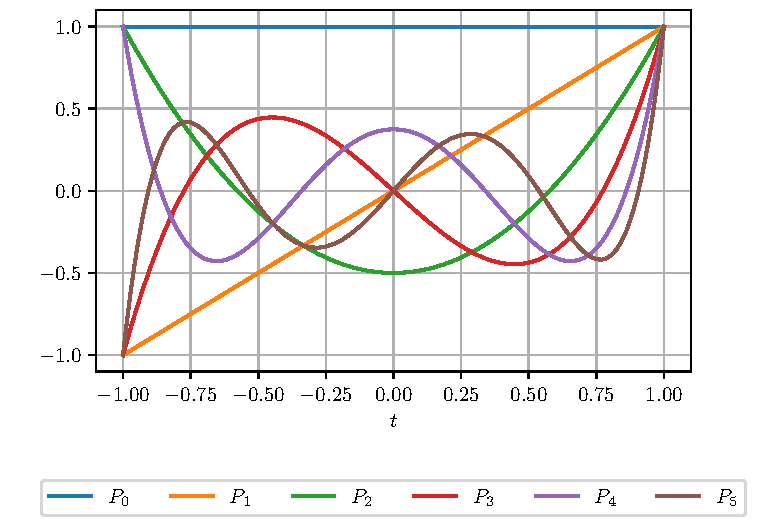
\includegraphics{./fig-legendre-polynomials.pdf}
\caption{Legendreove polynómy.  Obrázok bol pripravený Zdrojovým
kódom~\ref{src:lp} z~Prílohy~\ref{app:lp}.}
\label{fig:lp}
\end{figure}

V~Kapitole~\ref{sec:sh_motivation} sme ukázali, že ľubovoľný vektor~$\vec r$
z~trojrozmerného karteziánskeho súradnicového systému je možné popísať pomocou
jednotkových vektorov~$\vec e_i$, $i = 1, 2, 3$.  Obdobne je možné pomocou
niektorých systémov funkcií popísať každú spojitú funkciu~$f(t)$ na intervale
$t \in [1, 1]$.  Jeden z~takýchto systémov funkcií predstavujú práve
Legendreove polynómy~$P_n(t)$.

Rovnica
%
\begin{equation}
\label{eq:f_synthesis}
f(t) = \sum_{n = 0}^\infty \frac{2n + 1}{2} \, f_n \, P_n(t)
\end{equation}
%
umožňuje rozvinúť každú spojitú funkciu~$f(t)$ do radu Legendreových polynómov
pre ľubovoľné $t \in [-1, 1]$.  Vzťah~(\ref{eq:f_synthesis}) je možné vnímať aj
ako analógiu vzťahu~(\ref{eq:r_synthesis}), pričom~$f_n$ sú súradnice funkcie
$f(t)$ a~Legendreove polynómy~$P_n(t)$ plnia podobnú úlohu ako jednotkové
vektory~$\vec e_i$.  Konštanty~$f_n$ sú dané skalárnym súčinom funkcií~$f(t)$
a~$P_n(t)$ (porovnaj s~\ref{eq:r_analysis}),
%
\begin{equation}
\label{eq:f_analysis}
f_n = \int\limits_{-1}^1 f(t) \, P_n(t) \, \diff t{.}
\end{equation}
%
Dôkaz platnosti rovníc~(\ref{eq:f_synthesis}) a~(\ref{eq:f_analysis}) je možné 
nájsť napríklad vo \textcite{Freeden2009} či 
v~\textcite{SansoGeoidDetermination}.

Podobne ako skalárny súčin dvoch rôznych jednotkových vektorov~$\vec e_i$ 
a~$ \vec e_j$ je nulový (rovnica~\ref{eq:ei_orthogonality}), nulový je 
i~skalárny súčin dvoch rôznych Legendreovych polynómov~$P_n(t)$ a~$P_l(t)$,
%
\begin{equation}
\label{eq:lp_orthogonality}
\int\limits_{-1}^1 P_n(t) \, P_l(t) \, \diff t = 0{,} \quad n \neq l{.}
\end{equation}
%
Hovoríme preto, podobne ako v~súvislosti s~jednotkovými vektormi, že
\emph{Legendreove polynómy sú ortogonálne} na intervale $t \in [-1, 1].$
Rovnicu~(\ref{eq:lp_orthogonality}) možno zovšeobecniť doplnením prípadu~$n
= l$ \parencite[napríklad][]{Hobson},
%
\begin{equation}
\label{eq:lp_orthogonality_2}
\int\limits_{-1}^1 P_n(t) \, P_l(t) \, \diff t = \frac{2}{2n + 1} \, 
\delta_{nl}{.}
\end{equation}

Rovnice~(\ref{eq:f_synthesis}) a~(\ref{eq:f_analysis}) sú vo fyzikálnej
geodézii veľmi často využívané a~v~istej miere sme sa s~nimi stretli už
v~predchádzajúcej kapitole.  Nech~$r$ a~$r_Q$ z~rovnice~(\ref{eq:1l_legpol}) sú 
konštanty, pre ktoré platí~$r > r_Q$ (pozri podmienku
$\alpha < 1$ v~rovnici~\ref{eq:generic_function_for_lps}).  Keď označíme $f(t)
= 1 \slash l(t)$, $t = \cos\psi$, pomocou rovníc~(\ref{eq:lp_orthogonality_2})
a~(\ref{eq:1l_legpol}) sa môžeme presvedčiť, že koeficienty~$f_n$
z~rovnice~(\ref{eq:f_analysis}) sú dané vzťahom
%
\begin{equation}
f_n = \frac{1}{r_Q} \, \frac{2}{2n + 1} \, \left( \frac{r_Q}{r} \right)^{n
+ 1}{.}
\end{equation}
%
Dosadením týchto koeficientov do vzťahu~(\ref{eq:f_synthesis}) získame pôvodný 
vzťah~(\ref{eq:1l_legpol}).  Hoci ide o~triviálny príklad, demonštruje 
rozvinutie funkcie do radu Legendreových polynómov.  Takéto rozvinutie funkcie 
$f(t)$ pomocou Legendreových polynónom~$P_n(t)$ je v~istom zmysle obdobné 
vyjadreniu vektora~$\vec r$ pomocou jednotkových vektorov~$\vec e_i$ 
z~Kapitoly~\ref{sec:sh_motivation}.  Tento rozvoj je v~mnohých situáciách 
výhodný, pretože môže napríklad zjednodušiť odvodenie.  Napokon, najlepšie to 
demonštruje azda samotná Kapitola~\ref{sec:vg_sh_expansion}, v~ktorej sme 
funkciu~$1 \slash l$ rozvinuli do radu Legendreových polynómov a~následne 
Legendreových funkcií, čím sme získali vzťah~(\ref{eq:vg_sh_no_norm}).

Z~vlastností Legendreových polynómov spomeňme ešte aspoň nasledovné
\parencite{Freeden2009},
%
\begin{align}
\label{eq:pn_property1}
P_n(1) &= 1{,}\\
%
\label{eq:pn_property2}
P_n(-t) &= (-1)^n \, P_n(t){,}\\
%
\label{eq:pn_property3}
|P_n(t)| \leq P_n(1) &= 1{,} \quad t \in [-1, 1]{,}\\
%
\label{eq:pn_property4}
P_n'(1) &= \frac{n \, (n + 1)}{2}{,}
\end{align}
%
kde $P_n'(t) = \diff P_n(t) \slash \diff t$.  Vzťahy~(\ref{eq:pn_property1}) až
(\ref{eq:pn_property4}) platia pre~$n \geq 0$.   Širokú škálu ďalších
vlastností Legendreovych polynómov, ich derivácií či integrálov je možné nájsť
napríklad v~prácach \textcite{Gradshteyn2007}, \textcite{Freeden2009}
a~\textcite{Olver2010}.

Na záver pre úplnosť dodajme, že vzťahy~(\ref{eq:f_synthesis})
a~(\ref{eq:f_analysis}) možno aplikovať nielen na spojité funkcie~$f(t)$ na
intervale $t \in [-1, 1]$, ale i~na širšiu množinu funkcií.  Podrobnosti možno
nájsť napríklad v~prácach \textcite{Freeden2009} či \textcite{Arfken2005}.






\section{Legendreove funkcie}
\label{sec:legendre_functions}

Dosadením Rodriguesovho vzorca~(\ref{eq:pn_rodrigues}) do~(\ref{eq:pnm_def})
získame vzťah pre Legendreove funkcie,
%
\begin{equation}
\label{eq:pnm_ferrer}
P_{nm}(t) = \frac{1}{2^n \, n!} (1 - t^2)^{ m \slash 2} \, \frac{\diff^{n + m}
(t^2 - 1)^n}{\diff t^{n + m}}{.}
\end{equation}
%
Existuje tiež explicitný vzťah \parencite{Freeden2009},
%
\begin{equation}
P_{nm}(t) = \frac{1}{2^n}(1 - t^2)^{m \slash 2} \sum_{s = 0}^{\left\lfloor
\frac{n - m}{2} \right\rfloor} (-1)^s \, \frac{(2n - 2s)!}{s! \, (n - s)! \, (n
- m - 2s)!} \, t^{n - m - 2s}{,}
\end{equation}
%
či
%
množstvo rekurentných vzorcov, napríklad \parencite{Freeden2009}
%
\begin{equation}
\label{eq:pnm_recurrence}
P_{nm}(t) = \frac{2n - 1}{n - m} \, t \, P_{n - 1, m}(t) + \frac{n + m - 1}{n
- m} \, P_{n - 2, m}(t){.}
\end{equation}
%
Niekoľko prvých Legendreových funkcií má nasledovný tvar
(Obrázok~\ref{fig:lf}),
%
\begin{equation}
\label{eq:lf00_to_lf22}
\begin{split}
P_{0,0}(t) & = 1{,}\\
P_{1,0}(t) & = t{,}\\
P_{1,1}(t) & = \sqrt{1 - t^2}{,}\\
P_{2,0}(t) & = \frac{1}{2}(3t^2 - 1){,}\\
P_{2,1}(t) & = 3t \, \sqrt{1 - t^2}{,}\\
P_{2,2}(t) & = 3(1 - t^2){.}\\
\end{split}
\end{equation}

\begin{figure}[bt]
\centering
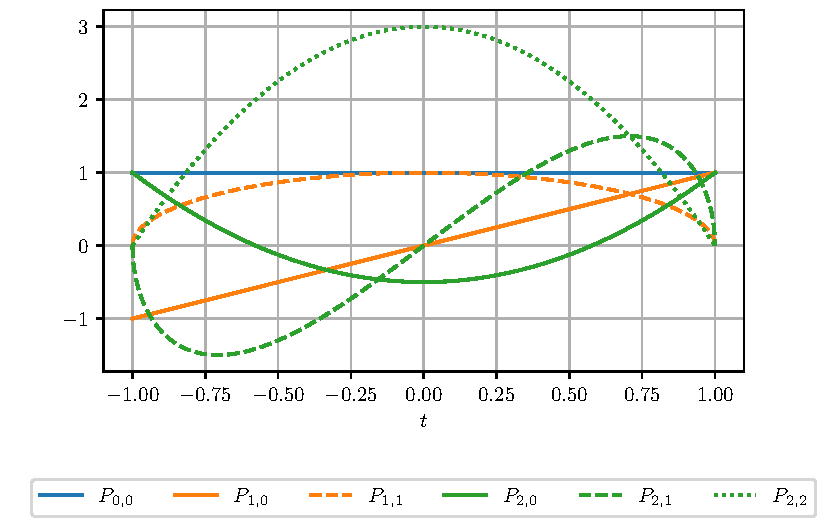
\includegraphics{./fig-legendre-functions.pdf}
\caption{Legendreove funkcie.}
\label{fig:lf}
\end{figure}

Legendreove funkcie rôznych stupňov~$n$, $l$ a~rovnakého rádu~$m$ sú
ortogonálne \parencite{Freeden2009},
%
\begin{equation}
\label{eq:pnm_orthogonality}
\int\limits_{-1}^{1} P_{nm}(t) \, P_{lm}(t) \, \diff t = 0{,} \quad n \neq l{.}
\end{equation}
%
Pre dve Legendreove funkcie rovnakého stupňa a~rádu platí
\begin{equation}
\label{eq:pnm_times_pnm}
\int\limits_{-1}^{1} P^2_{nm}(t) \, \diff t = \frac{2}{2n + 1} \, \frac{(n 
+ m)!}{(n - m)!}{.}
\end{equation}

Legendreove funkcie vyhovujú diferenciálnej rovnici druhého rádu 
\parencite{SansoGeoidDetermination}
%
\begin{equation}
\label{eq:legfunc1_differential_equation}
(1 - t^2) \, \frac{\diff^2 P_{nm}(t)}{\diff t^2} - 2 \, t \, \frac{\diff 
P_{nm}(t)}{\diff t} + \left[ n \, (n + 1) - \frac{m^2}{1 - t^2} \right] \, 
P_{nm}(t) = 0{.}
\end{equation}
%
Rovnica~(\ref{eq:legfunc1_differential_equation}) sa nazýva \emph{Legendreova 
diferenciálna rovnica}.  Dosadením~$m = 0$ 
do~(\ref{eq:legfunc1_differential_equation}) získame diferenciálnu rovnicu 
druhého rádu pre Legendreove polynómy,
%
\begin{equation}
\label{eq:legpol_differential_equation}
(1 - t^2) \, \frac{\diff^2 P_n(t)}{\diff t^2} - 2 \, t \, \frac{\diff 
P_n(t)}{\diff t} + n \, (n + 1) \, P_n(t) = 0{.}
\end{equation}

Na záver spomeňme ešte aspoň dve ďalšie vlastnosti Legendreových funkcií,
%
\begin{align}
\label{eq:pnm_symmetry}
P_{nm}(-t) &= (-1)^{n + m} \, P_{nm}(t){,}\\
%
P_{nm}(\pm1) &= 0{,} \quad m \neq 0{.}
\end{align}

Numerický výpočet Legendreových funkcií je zvyčajne uskutočňovaný rekurentnými 
vzťahmi.  Ide však o~netriviálnu úlohu, obzvlášť pre vysoké stupne a~rády 
\parencite{Holmes2002a,Fukushima2012a,Ishioka2018}.  
Vlastnosť~(\ref{eq:pnm_symmetry}) je preto výhodná; ak potrebujeme vypočítať 
$P_{nm}(\sin\varphi)$ a~$P_{nm}(\sin(-\varphi))$, rekurentné vzťahy môžeme 
aplikovať iba na získanie jedného z~týchto členov a~druhý člen dopočítame 
jednoduchým vzťahom~(\ref{eq:pnm_symmetry}).

\subsection{Condonov--Shortleyho fázový faktor}
\label{sec:legendre_functions_cs_factor}

V geodézii a~geomagnetizme sú Legendreove funkcie definované takmer výhradne 
vzťahom~(\ref{eq:pnm_ferrer}).  V~iných vedných odboroch, napríklad fyzike či 
seizmológii, sa používa definícia, ktorá obsahuje člen $(-1)^m$ 
\parencite[pozri][]{Wieczorek2015,Olver2010},
%
\begin{equation}
\begin{split}
P_n^m(t) &= (-1)^m \, (1 - t^2)^{m \slash 2} \, \frac{\diff^m P_n(t)}{\diff 
t^m}\\
%
&= \frac{(-1)^m}{2^n \, n!} (1 - t^2)^{ m \slash 2} \, \frac{\diff^{n + m}
(t^2 - 1)^n}{\diff t^{n + m}}{.}
\end{split}
\end{equation}
%
V~takom prípade sa rád Legendreovej funkcie $m$ zvykne zapisovať do horného 
indexu.  Člen $(-1)^{m}$ sa nazýva Condonov--Shortleyho fázový faktor.  Medzi 
$P_{nm}(t)$ a~$P_n^m(t)$ platí vzťah
%
\begin{equation}
P_{nm}(t) = (-1)^m \, P_n^m(t){.}
\end{equation}
%
V ďalších častiach práce budeme používať iba Legendreove funkcie $P_{nm}(t)$ 
definované vzťahom~(\ref{eq:pnm_ferrer}).




\section{Sférické harmonické funkcie}
\label{sec:spherical_harmonics}

V~rovnici~(\ref{eq:vg_sh_no_norm}) zaveďme substitúciu pre členy, ktoré závisia
iba od uhlovej časti sférických súradníc,
%
\begin{equation}
\label{eq:ynk_no_norm}
Y_{nk}(\varphi, \lambda) = P_{n|k|}(\sin\varphi)
%
\begin{cases}
\cos(k\lambda){,}    &\text{ak} \quad k \geq 0{,}\\
\sin(|k|\lambda){,}  &\text{ak} \quad k < 0{,}\\
\end{cases}
\end{equation}
%
pričom $n = 0, 1, 2, \dots$ a~$k = -n, \dots, n$.  Funkcia $Y_{nk}(\varphi,
\lambda)$ sa nazýva \emph{plošná sférická harmonická funkcia stupňa $n$ a~rádu
$k$}.

\begin{figure}[bt]
\centering
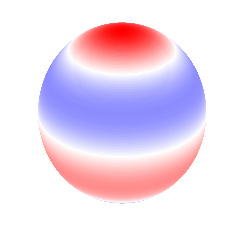
\includegraphics{./fig-spherical-harmonic-n3-k0.pdf}
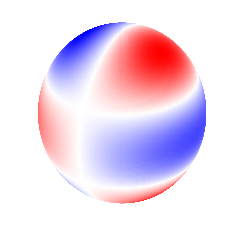
\includegraphics{./fig-spherical-harmonic-n3-k1.pdf}
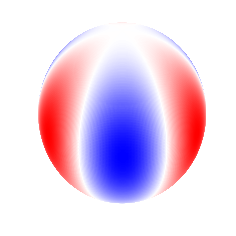
\includegraphics{./fig-spherical-harmonic-n3-k3.pdf}
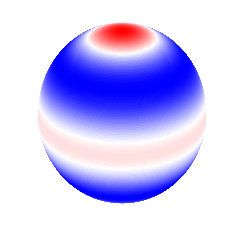
\includegraphics{./fig-spherical-harmonic-n4-k0.pdf}
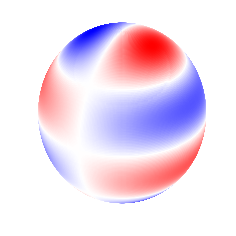
\includegraphics{./fig-spherical-harmonic-n4-k1.pdf}
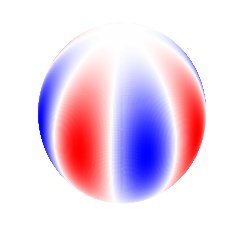
\includegraphics{./fig-spherical-harmonic-n4-k4.pdf}
\caption{Plošné sférické harmonické funkcie $Y_{nk}(\varphi, \lambda)$.
Záporné hodnoty sú zobrazené odtieňmi modrej farby, kladné hodnoty odtieňmi
červenej farby.  \textit{Vrchný rad} (zľava): $Y_{3,0}(\varphi, \lambda)$,
$Y_{3,1}(\varphi, \lambda)$, $Y_{3,3}(\varphi, \lambda)$.  \textit{Spodný rad}
(zľava): $Y_{4,0}(\varphi, \lambda)$, $Y_{4,1}(\varphi, \lambda)$,
$Y_{4,4}(\varphi, \lambda)$.  Obrázok bol pripravený Zdrojovým
kódom~\ref{src:ynk} z~Prílohy~\ref{app:sh}.}
\label{fig:sh}
\end{figure}

\begin{figure}[bt]
\centering
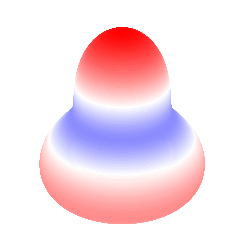
\includegraphics{./fig-spherical-harmonic-n3-k0-3d.pdf}
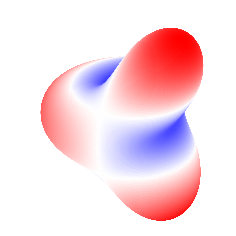
\includegraphics{./fig-spherical-harmonic-n3-k1-3d.pdf}
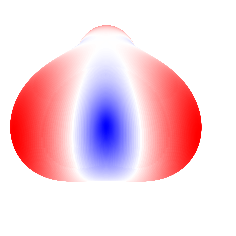
\includegraphics{./fig-spherical-harmonic-n3-k3-3d.pdf}
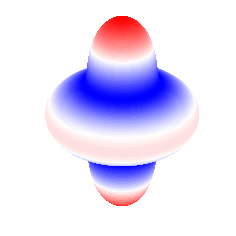
\includegraphics{./fig-spherical-harmonic-n4-k0-3d.pdf}
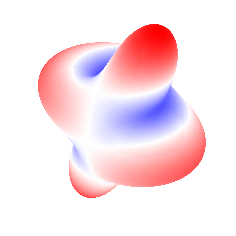
\includegraphics{./fig-spherical-harmonic-n4-k1-3d.pdf}
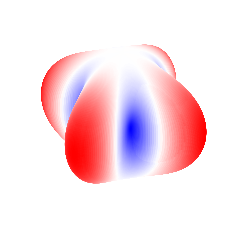
\includegraphics{./fig-spherical-harmonic-n4-k4-3d.pdf}
\caption{Plošné sférické harmonické funkcie $Y_{nk}(\varphi, \lambda)$
z~Obrázku~\ref{fig:sh} zobrazené odľahlosťou nadobúdanej hodnoty od jednotkovej
sféry.  Obrázok bol pripravený Zdrojovým kódom~\ref{src:ynk}
z~Prílohy~\ref{app:sh}.}
\label{fig:sh3d}
\end{figure}

Grafická reprezentácia sférických harmonických funkcií je uvedená na 
Obrázkoch~\ref{fig:sh} a~\ref{fig:sh3d}.  Možno si všimnúť, že sférické 
harmonické funkcie stupňa~$n$ a~rádu $k = 0$ (ľavý stĺpec na obrázkoch) menia 
$n$-krát znamienko v~smere sférickej šírky a~nezávisia od sférickej dĺžky.  Obe 
vlastnosti môžu byť overené dosadením~$k = 0$ do rovnice~(\ref{eq:ynk_no_norm}) 
(pozri tiež Kapitolu~\ref{sec:legendre_polynomials} a~Obrázok~\ref{fig:lp}),
%
\begin{equation}
\label{eq:yn0}
Y_{n0}(\varphi, \lambda) = P_n(\sin\varphi){.}
\end{equation}
%
Funkcia~$Y_{n0}(\varphi, \lambda)$ je symetrická voči rovine rovníka, ak $n 
= 0, 2, 4, \dots$ a~nesymetrická, ak $n = 1, 3, 5, \dots$ (pozri 
rovnicu~\ref{eq:yn0} a~vlastnosti Legendreových polynómov 
v~Kapitole~\ref{sec:legendre_polynomials}). Funkcie~$Y_{n0}(\varphi, \lambda)$ 
sa nazývajú \emph{zonálne sférické harmonické funkcie}.

Ak $0 < |k| < n$ (prostredný stĺpec na obrázkoch), sférická harmonická funkcia
mení znamienko s~oboma súradnicami.  V~smere sférickej šírky dochádza k~$n
- |k|$ zmenám znamienka.  Počet $n - |k|$ vyplýva z~$|k|$-tej derivácie
Legendreovho polynómu $P_n(\sin\varphi)$ (pozri rovnice~\ref{eq:pnm_def}
a~\ref{eq:pnm_ferrer}).  Deriváciou polynómu sa znižuje jeho stupeň, a~teda aj
počet možností meniť znamienko.  V~smere sférickej dĺžky sa znamienko mení
$2|k|$-krát, čo vyplýva z~vlastností trigonometrických funkcií
$\cos(k\lambda)$ a~$\sin(|k|\lambda)$.  Sférická harmonická funkcia rádu $0
< |k| < n$ má prívlastok \emph{teserálna}.

Ak $|k| = n$ (pravý stĺpec na obrázkoch), sférická harmonická funkcia
mení znamienko $0$-krát v~smere sférickej šírky, pretože $n - |k| = n - n = 0$,
a~$2|k|$-krát v~smere sférickej dĺžky.  Takáto funkcia sa nazýva
\emph{sektorálna sférická harmonická funkcia}.

Podobne ako jednotkové vektory, Legendreove polynómy či niektoré Legendreove
funkcie, i~sférické harmonické funkcie sú ortogonálne.  Táto vlastnosť vyplýva
z~nulového skalárneho súčinu dvoch rôznych sférických harmonických funkcií
$Y_{nk}(\varphi, \lambda)$ a~$Y_{rs}(\varphi, \lambda)$,
%
\begin{equation}
\label{eq:ynk_no_norm_orthogonality}
\iint\limits_{\sigma} Y_{nk}(\varphi, \lambda) \, Y_{rs}(\varphi, \lambda) \, 
\diff \sigma = 0{,}
\end{equation}
%
pričom buď $n \neq r$ alebo $k \neq s$ alebo platia obe podmienky súčasne.  Pre
skalárny súčin dvoch rovnakých sférických harmonických funkcií platí
%
\begin{equation}
\label{eq:ynk_times_ynk}
\iint\limits_{\sigma} Y_{nk}(\varphi, \lambda) \, Y_{nk}(\varphi, \lambda) \, 
\diff \sigma =
%
\dfrac{4\pi}{(2 - \delta_{k0}) \, (2n + 1)} \, \dfrac{(n + |k|)!}{(n
- |k|)!}{.}
\end{equation}
%
Overenie vzťahov~(\ref{eq:ynk_no_norm_orthogonality})
a~(\ref{eq:ynk_times_ynk}) ponecháme na čitateľa.  Je potrebné použiť
rovnice~(\ref{eq:pnm_orthogonality}), (\ref{eq:pnm_times_pnm}),
(\ref{eq:ynk_no_norm}) a~vypočítať integrály
%
\begin{equation}
\int\limits_{0}^{2\pi} \cos(k \lambda) \, \diff\lambda \quad \text{a} \quad
\int\limits_{0}^{2\pi} \sin(|k| \lambda) \, \diff\lambda{.}
\end{equation}
%
Vo vzťahoch~(\ref{eq:pnm_orthogonality}) a~(\ref{eq:pnm_times_pnm}) je potrebné
aplikovať substitúciu integračnej premennej,
%
\begin{equation}
\int\limits_{-1}^{1} P_{nm}(t) \, P_{rs}(t) \, \diff
t~= \int\limits_{-\frac{\pi}{2}}^{\frac{\pi}{2}} P_{nm}(\sin\varphi) \,
P_{rs}(\sin\varphi) \, \cos\varphi \, \diff \varphi{.}
\end{equation}


Nech $f(\varphi, \lambda)$ je funkcia na jednotkovej sfére $\sigma$.  Nech pre
$f(\varphi, \lambda)$ ďalej platí
%
\begin{equation}
\label{eq:f_l2}
\iint\limits_\sigma f^2(\varphi, \lambda) \, \diff \sigma < \infty{.}
\end{equation}
%
Podmienku~(\ref{eq:f_l2}) spĺňa napríklad každá spojitá funkcia na jednotkovej
sfére.  Každú takúto funkciu $f(\varphi, \lambda)$ možno rozvinúť do radu
sférických harmonických funkcií \parencite[napríklad][]{MoritzPhysicalGeodesy},
%
\begin{equation}
\label{eq:f_shs_no_norm}
f(\varphi, \lambda) = \sum_{n = 0}^\infty \sum_{k = -n}^n f_{nk} \,
Y_{nk}(\varphi, \lambda){.}
\end{equation}
%
Koeficienty $f_{nk}$ je možné získať nasledovne.  Vynásobme 
rovnicu~(\ref{eq:f_shs_no_norm}) sférickou harmonickou funkciou 
$Y_{rs}(\varphi, \lambda)$ a~následne rovnicu zintegrujme na jednotkovej sfére 
$\sigma$.  Použitím vzťahov~(\ref{eq:ynk_no_norm_orthogonality}) 
a~(\ref{eq:ynk_times_ynk}) získame hľadané koeficienty
%
\begin{equation}
\label{eq:f_sha_no_norm}
f_{nk} = \frac{(2 - \delta_{k0}) \, (2n + 1)}{4\pi} \, \frac{(n - |k|)!}{(n 
+ |k|)!} \, \iint\limits_{\sigma} f(\varphi, \lambda) \, Y_{nk}(\varphi, 
\lambda) \, \diff \sigma{.}
\end{equation}

Vidíme teda, že ak je splnená podmienka~(\ref{eq:f_l2}), potom možno 
funkciu~$f(\varphi, \lambda)$ rozložiť pomocou sférických harmonických funkcií 
na súradnice $f_{nk}$ (rovnica~\ref{eq:f_sha_no_norm}) a~následne ju spätne 
zrekonštruovať (vzťah~\ref{eq:f_shs_no_norm}).  V~priestore funkcií $f(\varphi, 
\lambda)$, ktoré sú definované na sfére a~spĺňajú podmienku~($\ref{eq:f_l2}$), 
plnia sférické harmonické funkcie $Y_{nk}(\varphi, \lambda)$ podobnú úlohu ako 
plnia jednotkové vektory $\vec e_i$ v~priestore trojrozmerných vektorov $\vec 
r$.  Funkcia $f(\varphi,\lambda)$ môže byť napríklad gravitačný či magnetický 
potenciál telesa na sfére, ktorá obopína celé teleso, topografia Zeme či inej 
planéty a~množstvo ďalších funkcií.  Každú takúto funkciu možno rozvinúť do 
vlastného radu sférických harmonických funkcií (vzťah~\ref{eq:f_shs_no_norm}), 
pričom každá funkcia bude mať vlastné súradnice $f_{nk}$, podobne ako každý 
vektor $\vec r$ má vlastné súradnice $r_i$.  Všimnime si, že ak označíme
%
\begin{equation}
\label{eq:sh_norm}
N_{n|k|} = \sqrt{(2 - \delta_{k0}) (2n + 1) \, \frac{(n - |k|)!}{(n
+ |k|)!}}{,}
\end{equation}
%
potom vzťahy~(\ref{eq:f_sha_no_norm}) a~(\ref{eq:f_shs_no_norm}) sú totožné so
vzťahmi~(\ref{eq:vg_analysis}) a~(\ref{eq:vg_synthesis}) pre $r = 1$.



\section{Normovanie}
\label{sec:normalization}

V~praktických aplikáciách sa sférické harmonické funkcie zvyknú definovať tak, 
že sú vynásobené členom, ktorý závisí od sférického harmonického stupňa a~rádu.  
Tento člen sa nazýva \emph{norma} a~jeho použitím dostaneme \emph{normované 
sférické harmonické funkcie}.  Normovaním získame niektoré vlastnosti, ktoré sú 
výhodne z~teoretického aj z~praktického hľadiska.  Tieto vlastnosti budú 
podrobnejšie diskutované v~Kapitolách~\ref{sec:leg_sh_norm} 
a~\ref{sec:shc_norm}.  Existuje niekoľko typov noriem, napríklad Schmidtova 
polovičná norma, ortonormálna norma či úplná norma \parencite{SHTOOLS}.  
V~geodézii sa používa takmer výhradne úplná norma, preto sa budeme venovať iba 
jej.

\subsection{Legendreove funkcie a~sférické harmonické funkcie}
\label{sec:leg_sh_norm}

Pre skalárny súčin dvoch rovnakých jednotkových vektorov $\vec e_i$ platí 
vzťah~(\ref{eq:ei_unit_length}).  Z~teoretického aj z~praktického hľadiska by 
bolo výhodné, aby aj skalárny súčin dvoch rovnakých sférických harmonických 
funkcií bol rovný~$1$.  Túto vlastnosť možno zabezpečiť vynásobením 
Legendreových funkcií $P_{nm}(\sin\varphi)$ členom $N_{n|k|}$ 
(rovnica~\ref{eq:sh_norm}), ktorý nazývame \emph{úplná norma}.  Získame tým 
\emph{úplne normované Legendreove funkcie},
%
\begin{equation}
\bar{P}_{nm}(\sin\varphi) = N_{nm} \, P_{nm}(\sin\varphi){,} \quad  n = 0, 1, 
\dots,
\quad m = 0, 1, \dots, n{,}
\end{equation}
%
a~\emph{úplne normované sférické harmonické funkcie}
%
\begin{equation}
\label{eq:ynk_norm}
\begin{split}
\bar{Y}_{nk}(\varphi, \lambda) = N_{n|k|} \, Y_{nk}(\varphi, \lambda)
= \bar{P}_{n|k|}(\sin\varphi)
%
\begin{cases}
\cos(k\lambda){,}    &\text{ak} \quad k \geq 0{,}\\
\sin(|k|\lambda){,}  &\text{ak} \quad k < 0{,}
\end{cases}
&
%
\\
n = 0, 1, \dots, \quad k = -n, \dots, n{.}&
\end{split}
\end{equation}
%
Použitím normy~(\ref{eq:sh_norm}) je možné podobne ako 
v~rovnici~(\ref{eq:ynk_no_norm_orthogonality}) ukázať, že platí
%
\begin{equation}
\label{eq:ynk_norm_orthogonality}
\frac{1}{4\pi} \, \iint\limits_{\sigma} \bar{Y}_{nk}(\varphi, \lambda) \,
\bar{Y}_{rs}(\varphi, \lambda) \, \diff \sigma = \delta_{nr} \, \delta_{ks}{.}
\end{equation}
%
Skalárny súčin~(\ref{eq:ynk_norm_orthogonality}) dvoch rôznych úplne
normovaných sférických harmonických funkcií je teda rovný 0, zatiaľ čo skalárny
súčin dvoch rovnakých úplne normovaných sférických harmonických funkcií je
rovný $1$.

Vzťahy~(\ref{eq:f_shs_no_norm}) a~(\ref{eq:f_sha_no_norm}) potom prejdu do
tvaru
%
\begin{align}
\label{eq:f_shs}
f(\varphi, \lambda) &= \sum_{n = 0}^\infty \sum_{k = -n}^n \bar{f}_{nk} \,
\bar{Y}_{nk}(\varphi, \lambda){,}\\
%
\label{eq:f_sha}
\bar{f}_{nk} &= \frac{1}{4\pi} \, \iint\limits_{\sigma} f(\varphi, \lambda) \,
\bar{Y}_{nk}(\varphi, \lambda) \, \diff \sigma{.}
\end{align}
%
Úplne normované sférické harmonické funkcie tiež umožňujú zapísať dekompozičný
teorém~(\ref{eq:pn_decomposition_formula}) v~tvare
\parencite{MoritzPhysicalGeodesy}
%
\begin{equation}
P_n(\cos\psi) = \frac{1}{2n + 1} \, \sum_{k = -n}^n \bar{Y}_{nk}(\varphi,
\lambda) \, \bar{Y}_{nk}(\varphi_Q, \lambda_Q)
\end{equation}
%
a~prevrátenú hodnotu vzdialenosti $1 \slash l$ z~rovnice~(\ref{eq:1l}) v~tvare
%
\begin{equation}
\label{eq:1l_sh}
\frac{1}{l} = \frac{1}{r_Q} \, \sum_{n = 0}^{\infty} \frac{1}{2n + 1} \, \left( 
\frac{r_Q}{r} \right)^{n + 1} \, \sum_{k = -n}^n \bar{Y}_{nk}(\varphi,
\lambda) \, \bar{Y}_{nk}(\varphi_Q, \lambda_Q){.}
\end{equation}
%

Z~numerického hľadiska je výpočet nenormovaných Legendreových funkcií 
problematický, a~to už i~pre stupne a~rády presahujúce niekoľko stoviek.  
Dôvodom je ich pomerne rýchlo narastajúca hodnota, ktorá dokonca prekročí 
rozsah dvojitej presnosti.  Dvojitá presnosť je v~súčasnosti najčastejšie 
používaný štandard na počítačovú reprezentáciu čísel s~pohyblivou desatinnou 
čiarkou.  Číslo väčšie ako horný rozsah dvojitej presnosti je v~dvojitej 
presnosti reprezentované nekonečnom.  Z~tohto dôvodu je z~praktického hľadiska 
výhodnejšie pracovať s~úplne normovanými Legendreovými funkciami.  Kvôli 
opísaným numerickým problémom sa však nepočíta zvlášť norma $N_{nm}$ a~zvlášť 
nenormovaná Legendreova funkcia $P_{nm}(\sin\varphi)$, ale počítajú sa priamo 
úplne normované Legendreove funkcie $\bar{P}_{nm}(\sin\varphi)$ pomocou 
upravených rekurentných vzťahov (pozri napríklad \cite{Holmes2002a} či 
\cite{Fukushima2012a}).



\subsection{Sférické harmonické koeficienty}
\label{sec:shc_norm}

Sférické harmonické koeficienty $C_{nm}$ a~$S_{nm}$ zo
vzťahu~(\ref{eq:vg_sh_no_norm}) sú zvyčajne normované dvakrát.  Prvá norma
zabezpečuje ich bezrozmernosť, druhá norma je potrebná v~dôsledku normovania 
sférických harmonických funkcií~(Kapitola~\ref{sec:leg_sh_norm}).

Fyzikálna jednotka koeficientov $C_{nm}$ a~$S_{nm}$
z~rovnice~(\ref{eq:vg_shc_no_norm}) je $\mathrm{m}^n \, \mathrm{kg}$ a~závisí 
od stupňa~$n$.  Je preto výhodne koeficienty normovať tak, aby boli
bezrozmerné.  Norma zaužívaná v~geodézii má tvar
%
\begin{equation}
\label{eq:cnm_snm_1st_norm}
\begin{rcases}
\tilde{C}_{nm}\\
\tilde{S}_{nm}
\end{rcases}
= \frac{1}{M \, R^n}
\begin{cases}
C_{nm}{,}\\
S_{nm}{,}
\end{cases}
\end{equation}
%
kde $M$ je hmotnosť telesa, ktoré generuje gravitačný potenciál a~$R$ je
polomer najmenšej sféry, v~ktorej sa nachádza celé teleso, $R
= \max(r_\mathrm{S}(\varphi_Q, \lambda_Q))$.  Vzťah~(\ref{eq:vg_sh_no_norm})
potom prejde do tvaru
%
\begin{equation}
\label{eq:vg_sh_1st_norm}
V_\gidx(P) = \frac{GM}{R} \sum_{n = 0}^\infty \left( \frac{R}{r} \right)^{n
+ 1} \sum_{m = 0}^{n} \left( \tilde{C}_{nm} \, \cos(m\lambda) + \tilde{S}_{nm}
\, \sin(m\lambda)\right) \, P_{nm}(\sin\varphi){.}
\end{equation}

Ak sú sférické harmonické funkcie normované členom $N_{n|k|}$ (pozri 
rovnicu~\ref{eq:sh_norm}), potom sférické harmonické koeficienty musia byť 
normou $N_{n|k|}$ vydelené, aby sa zachovala rovnosť vo 
vzťahoch~(\ref{eq:vg_sh_no_norm}) a~(\ref{eq:vg_sh_1st_norm}).  Druhá norma 
sférických harmonických koeficientov je preto daná nasledovne,
%
\begin{equation}
\label{eq:cnm_snm_2nd_norm}
\begin{rcases}
\bar{C}_{nm}\\
\bar{S}_{nm}
\end{rcases}
= \frac{1}{N_{nm}}
\begin{cases}
\tilde{C}_{nm}{,}\\
\tilde{S}_{nm}{.}
\end{cases}
\end{equation}
%
Sférický harmonický rozvoj~(\ref{eq:vg_sh_1st_norm}) následne prejde do tvaru
%
\begin{equation}
\label{eq:vg_sh_2nd_norm}
V_\gidx(P) = \frac{GM}{R} \sum_{n = 0}^\infty \left( \frac{R}{r} \right)^{n
+ 1} \sum_{m = 0}^{n} \left( \bar{C}_{nm} \, \cos(m\lambda) + \bar{S}_{nm} \,
\sin(m\lambda)\right) \, \bar{P}_{nm}(\sin\varphi){.}
\end{equation}
%
Ekvivalentný, no úspornejší zápis dosiahneme použitím substitúcie
$\bar{Y}_{nk}(\varphi, \lambda)$,
%
\begin{equation}
\label{eq:vg_sh_2nd_norm_ynk}
V_\gidx(P) = \frac{GM}{R} \sum_{n = 0}^\infty \left( \frac{R}{r} \right)^{n
+ 1} \sum_{k = -n}^{n} \bar{v}_{nk} \, \bar{Y}_{nk}(\varphi, \lambda){,}
\end{equation}
kde
%
\begin{equation}
\bar{v}_{nk} =
%
\begin{cases}
\bar{C}_{nk}{,}    &\text{ak} \quad k \geq 0{,}\\
\bar{S}_{n|k|}{,}  &\text{ak} \quad k < 0{.}\\
\end{cases}
\end{equation}
%
Koeficienty $\bar{C}_{nm}$ a~$\bar{S}_{nm}$, resp. $\bar{v}_{nk}$, sa nazývajú
\emph{úplne normované sférické harmonické koeficienty}.

Podobne ako úplne normované Legendreove funkcie, ani sférické
harmonické koeficienty sa nezvyknú počítať samostatne od normy.  Namiesto toho
sa vypočítajú úplne normované sférické harmonické funkcie
$\bar{Y}_{nk}(\varphi, \lambda)$ a~následne sa napríklad
vzťahom~(\ref{eq:f_sha}) získajú priamo úplne normované sférické harmonické
koeficienty.





% -----------------------------------------------------------------------------

\section{Fyzikálnych význam niektorých sférických harmonických koeficientov}
\label{sec:physical_meaning_of_spherical_harmonic_coefficients}

Dosaďme $P_{0,0}(\sin\varphi)$ z~rovnice~(\ref{eq:lf00_to_lf22})
do rovnice~(\ref{eq:vg_shc_no_norm}) pre $n = 0$ a~$m = 0$,
%
\begin{equation}
\label{eq:c00_mass}
C_{0,0} = \iiint\limits_{\tau} \rho(Q) \, \diff \tau(Q) = M{.}
\end{equation}
%
Nenormovaný koeficient $C_{0,0}$ má teda fyzikálny význam, je rovný hmotnosti 
telesa~$M$.  Ak obmedzíme nekonečné rady~(\ref{eq:vg_sh_no_norm}), 
(\ref{eq:vg_sh_1st_norm}), (\ref{eq:vg_sh_2nd_norm}) či 
(\ref{eq:vg_sh_2nd_norm_ynk}) na maximálny stupeň $N = 0$, získame vzťah
%
\begin{equation}
\label{eq:vg_sh_0degree}
V_\gidx(P) = \frac{GM}{r}{.}
\end{equation}
%
Rovnica~(\ref{eq:vg_sh_0degree}) predstavuje gravitačný potenciál hmotného bodu
s~hmotnosťou $M$ vo vzdialenosti $r$ od hmotného bodu (pozri
rovnicu~\ref{eq:vg_point_mass}).  Pomocou Newtonovho
integrálu~(\ref{eq:vg_body}) možno ukázať, že gravitačný potenciál gule
s~konštantnou hustotou (homogénna guľa) je tiež ekvivalentný so
vzťahom~(\ref{eq:vg_sh_0degree}).  Preto ak obmedzíme nekonečný sférický
harmonický rozvoj gravitačného potenciálu na maximálny stupeň $N = 0$, získame
gravitačný potenciál homogénnej gule, ktorá nahrádza skutočné teleso.

Vydeľme rovnicu~(\ref{eq:vg_shc_no_norm}) hmotnosťou $M$ a~zopakujme postup pre
stupeň $n = 1$ a~rády $m = 0, 1$.  Po uvážení~(\ref{eq:sph2cart}) získame
%
\begin{equation}
\begin{split}
\frac{C_{1,0}}{M} &= \frac{1}{M} \iiint\limits_{\tau} \rho(Q) \, z_Q \, \diff 
\tau(Q) = z_\mathrm{c}{,}\\
\frac{C_{1,1}}{M} &= \frac{1}{M} \iiint\limits_{\tau} \rho(Q) \, x_Q \, \diff 
\tau(Q) = x_\mathrm{c}{,}\\
\frac{S_{1,1}}{M} &= \frac{1}{M} \iiint\limits_{\tau} \rho(Q) \, y_Q \, \diff 
\tau(Q) = y_\mathrm{c}{.}
\end{split}
\end{equation}
%
Súradnice $x_\mathrm{c}$, $y_\mathrm{c}$ a~$z_\mathrm{c}$ predstavujú posun
začiatku súradnicového systému voči ťažisku telesa.  V~praktických aplikáciách 
pracujeme veľmi často v~geocentrickom súradnicovom systéme so
začiatkom v~ťažisku Zeme, preto všetky koeficienty stupňa $n = 1$ sú zvyčajne
nulové, $C_{1,0} = C_{1,1} = S_{1,1} = 0$.

Je možné ukázať \parencite[napríklad][]{MoritzPhysicalGeodesy}, že koeficienty
stupňa $n = 2$ súvisia s~momentom zotrvačnosti.  Koeficienty vyšších stupňov
už, zdá sa, nemajú priamočiaru fyzikálnu interpretáciu.






% -----------------------------------------------------------------------------

\section{Aplikácie sférického harmonického rozvoja}
\label{sec:spherical_harmonics_applications}

V~tejto kapitole ukážeme dve typické aplikácie sférických harmonických rozvojov 
vo fyzikálnej geodézii, modelovanie vonkajšieho gravitačného 
poľa~(Kapitola~\ref{sec:sh_applications_gravity_field})
a~modelovanie topografie približne sférických 
telies~(Kapitola~\ref{sec:sh_applications_topography}).

\subsection{Gravitačné pole}
\label{sec:sh_applications_gravity_field}

Koeficienty $\bar{C}_{nm}$ a~$\bar{S}_{nm}$ je možné vypočítať napríklad
z~obežnej dráhy umelej družice Zeme.  Tak ako Slnko ovplyvňuje dráhu planéty
v~príklade z~Kapitoly~\ref{sec:newton_law}, podobne i~Zem vplýva na dráhu
družice prostredníctvom svojho gravitačného poľa.  Tentokrát je ale situácia
zložitejšia ako na Obrázku~\ref{fig:orbital_motion}, pretože družica obieha
okolo Zeme v~bezprostrednej blízkosti vo výške približne $250$~-- $500$~km nad
jej povrchom.  Keďže gravitačné pole Zeme sa v~priestore rôznorodo mení (pozri
Obrázky~\ref{fig:gg_grav_sr_2arcsec} a~\ref{fig:vg_grav_sr_2arcsec}), dráha
družice je ovplyvnená ináč v~oblasti so silným gravitačným poľom (napríklad nad
masívnymi pohoriami) a~ináč v~oblasti so slabším gravitačným poľom.  V~dôsledku
premenlivého gravitačného poľa Zeme preto družica neobieha po
elipse.\footnote{Dráhu družice ovplyvňujú aj iné faktory, napríklad tlak
slnečného žiarenia, odpor atmosféry a~pod.  Tieto vplyvy pre jednoduchosť
zanedbáme.}  Jej skutočná dráha je komplikovaná priestorová krivka,
reflektujúca gravitačné pole v~danej oblasti, a~elipsa je len jej priblíženie
(Obrázok~\ref{fig:orbital_motion_real}).  Ak by sme teda poznali skutočnú dráhu
družice, mali by sme byť schopní inverzným spôsobom vypočítať to pole, ktoré je
príčinou neeliptickej dráhy.  Inými slovami, zo skutočnej dráhy družice je
možné vypočítať sférické harmonické koeficienty $\bar{C}_{nm}$
a~$\bar{S}_{nm}$.  Koeficienty $\bar{C}_{nm}$ a~$\bar{S}_{nm}$ je možné
vypočítať i~z mnohých iných geodetických meraní, či už družicových alebo
pozemných.  Podrobnejšie informácie o~družicových misiách a~jednotlivých
technikách je možné nájsť napríklad v~prácach \textcite{SeeberSatelliteGeodesy}
a~\textcite{MoritzPhysicalGeodesy}.

\begin{figure}
\centering
\input{./fig-orbital-motion-real.pdf_tex}
\caption{Pohyb umelej družice Zeme.}
\label{fig:orbital_motion_real}
\end{figure}

V~Kapitole~\ref{sec:potential_theory} sme uviedli, že gravitačný potenciál 
obsahuje informáciu o~všetkých veličinách gravitačného poľa.  Zo 
vzťahu~(\ref{eq:vg_sh_2nd_norm}) je preto možné vyťažiť oveľa viac ako len 
informáciu o~gravitačnom potenciáli.  Napríklad aplikovaním operátora 
gradient~(\ref{eq:gradient_sph}) na gravitačný 
potenciál~(\ref{eq:vg_sh_2nd_norm}) možno získať prvky vektora gravitačného 
zrýchlenia v~lokálnom karteziánskom súradnicovom systéme s~pohyblivým začiatkom 
$x^\mathrm{s}$, $y^\mathrm{s}$, $z^\mathrm{s}$ (Obrázok~\ref{fig:cart_sph}),
%
\begin{align}
\label{eq:vgx_sh}
\left.\frac{\partial V_\gidx}{\partial x^\mathrm{s}}\right|_P &= \frac{1}{r} \, 
\left.\frac{\partial V_\gidx}{\partial \varphi}\right|_P\nonumber\\
%
&= \frac{GM}{R^2} \sum_{n = 0}^\infty \left( \frac{R}{r} \right)^{n + 2} 
\sum_{m = 0}^{n} \left(
\bar{C}_{nm} \, \cos(m\lambda) + \bar{S}_{nm} \, \sin(m\lambda)\right) \,
\frac{\diff \bar{P}_{nm}(\sin\varphi)}{\diff \varphi}{,}\displaybreak[2]\\
%
\label{eq:vgy_sh}
\left.\frac{\partial V_\gidx}{\partial y^\mathrm{s}}\right|_P &= \frac{1}{r \, 
\cos\varphi} \, \left.\frac{\partial V_\gidx}{\partial 
\lambda}\right|_P\nonumber\\
%
&= \frac{GM}{R^2 \, \cos\varphi} \sum_{n = 0}^\infty \left( \frac{R}{r} 
\right)^{n + 2} \sum_{m = 0}^{n}\left(
\bar{S}_{nm} \, \cos(m\lambda) - \bar{C}_{nm} \, \sin(m\lambda)\right) \, m \,
\bar{P}_{nm}(\sin\varphi){,}\displaybreak[2]\\
%
\label{eq:vgz_sh}
\left.\frac{\partial V_\gidx}{\partial z^\mathrm{s}}\right|_P &= 
\left.\frac{\partial V_\gidx}{\partial r}\right|_P\nonumber\\
%
&= - \frac{GM}{R^2} \sum_{n = 0}^\infty (n + 1) \, \left( \frac{R}{r} 
\right)^{n + 2} \sum_{m = 0}^{n}
\left( \bar{C}_{nm} \, \cos(m\lambda) + \bar{S}_{nm} \, \sin(m\lambda)\right)
\, \bar{P}_{nm}(\sin\varphi){.}
\end{align}
%
Sférickými harmonickými rozvojmi teda môžeme vypočítať prakticky akúkoľvek 
veličinu gravitačného či tiažového poľa, od gravitačného potenciálu, cez 
gravitačné zrýchlenie až po zvislicové odchýlky či geoid.  
Rovnice~(\ref{eq:vgx_sh}) až~(\ref{eq:vgz_sh}) tiež prakticky demonštrujú 
výhodnosť vyjadrenia operátora gradient vo sférických súradniciach 
(rovnica~\ref{eq:gradient_sph}).  Priamy výpočet derivácií $\partial V_\gidx 
\slash \partial x^\mathrm{s}$, $\partial V_\gidx \slash \partial y^\mathrm{s}$ 
a $\partial V_\gidx \slash \partial z^\mathrm{s}$ 
vzťahu~(\ref{eq:vg_sh_2nd_norm}) by bol náročný.

ICGEM (angl. \emph{International Centre for Global Earth Models}) je služba 
zriadená Medzinárodnou geodetickou asociáciou (angl.~\emph{International 
Association of Geodesy}, IAG).  Okrem iného je jej cieľom zbierať, archivovať 
a~poskytovať globálne modely gravitačného poľa Zeme, najčastejšie práve vo 
forme sférických harmonických koeficientov $\bar{C}_{nm}$ a~$\bar{S}_{nm}$.  Na 
jej domovskej stránke\footnote{\url{http://icgem.gfz-potsdam.de/home}} je možné 
nájsť desiatky sád sférických harmonických koeficientov, získané z~rôznych dát 
a~rozličnými metódami výpočtu.  Dostupné sú aj časovo premenlivé modely 
gravitačného poľa, služba na výpočet vzťahu~(\ref{eq:vg_sh_2nd_norm}) či modely 
gravitačného poľa nebeských telies (napríklad Mars, Venuša, Mesiac či asteroidy 
Slnečnej sústavy).

Služba ICGEM poskytuje modely v~štandardizovanom tvare v~textových súboroch 
s~príponou~\texttt{gfc}.  V~Prílohe~\ref{app:gfc_file} je uvedená ukážka~modelu 
s~názvom EIGEN-6C4 \parencite{EIGEN-6C4}.  Na začiatku \texttt{gfc} súborov sú 
spravidla uvedené stručné informácie o~poskytovanom modeli, najmä mená autorov 
modelu, dáta a~metódy použité na jeho výpočet a~odkazy na relevantnú odbornú 
literatúru.  Riadky s~kľúčovými slovami \texttt{earth\_gravity\_constant} 
a~\texttt{radius} v~hlavičke súboru udávajú hodnoty geocentrickej gravitačnej 
konštanty~$GM$ a~referenčného polomeru~$R$, ktoré sú spojené s~daným modelom.  
V~rovnici~(\ref{eq:vg_sh_2nd_norm_ynk}) a~jej rôznych podobách musia byť 
použité práve tieto hodnoty.  Všimnime si, že koeficient $\bar{C}_{0,0}$ modelu 
EIGEN-6C4 má hodnotu~$1$.  Je to spôsobené tým, že nenormovaný 
koeficient~$C_{0,0}$ je rovný hmotnosti Zeme (rovnica~\ref{eq:c00_mass}), avšak 
po aplikovaní prvej a~druhej normy~(rovnice~\ref{eq:cnm_snm_1st_norm} 
a~\ref{eq:cnm_snm_2nd_norm}) nadobudne hodnotu~$1$.  Môžeme si tiež všimnúť, že 
všetky koeficienty stupňa~$n = 1$ sú nulové, teda začiatok súradnicového 
systému modelu EIGEN-6C4 je vložený do ťažiska Zeme (pozri 
Kapitolu~\ref{sec:physical_meaning_of_spherical_harmonic_coefficients}).

Sférické harmonické koeficienty gravitačného poľa Zeme sú v~súčasnosti dostupné
približne do stupňa $2190$.  Získavané sú väčšinou kombináciou družicových
meraní (približne do stupňa $250$ až $300$) a~detailných pozemných
gravimetrických meraní (približne do stupňa $720$ až $2190$).  Existujú tiež 
modely, ktoré popisujú zemské gravitačné pole do vyšších stupňov ako $2190$.  
Tieto vysoké harmonické stupne však nie sú založené na meraniach zemského 
gravitačného poľa, ale na modelovaní gravitačného účinku topografických hmôt, 
ktoré sa nachádzajú nad geoidom \parencite[napríklad][]{Ince2020}.



\subsection{Topografia}
\label{sec:sh_applications_topography}

V~Kapitole~\ref{sec:spherical_harmonics} sme uviedli, že do radu sférických
harmonických funkcií je možné rozvinúť nielen gravitačný potenciál, ale každú
funkciu, ktorá spĺňa podmienku~(\ref{eq:f_l2}).  Rozviňme preto do stupňa~$N$ 
napríklad zemskú topografiu $H(\varphi, \lambda)$,
%
\begin{equation}
\label{eq:h_shs}
H(\varphi, \lambda) = \sum_{n = 0}^{N} \sum_{k = -n}^n \bar{h}_{nk} \,
\bar{Y}_{nk}(\varphi, \lambda){.}
\end{equation}
%
Obrázok~\ref{fig:shs_h} znázorňuje vplyv parametra~$N$ na priestorové 
rozlíšenie funkcie $H(\varphi, \lambda)$.  Koeficienty~$\bar{h}_{nk}$ boli 
prevzaté z~modelu~DTM2006.0 \parencite{DTM2006}.  Hoci všetky tri mapy sú 
vypočítané s~rovnakým vzorkovaním ($0.25^{\circ}$ vo sférickej šírke a~dĺžke), 
miera detailu stúpa od vrchnej mapy smerom nadol.  Spôsobené je to tým, že 
maximálny stupeň $N$, ktorý udáva priestorové rozlíšenie funkcie 
$H(\varphi,\lambda)$, narastá postupne od~$30$ cez~$90$ až do~$360$.  Odhad 
veľkosti najmenšieho priestorového prvku, ktorý môže byť reprezentovaný 
sférickým harmonickým rozvojom do stupňa~$N$, je možné vzťahom
%
\begin{equation}
l_{\min}(N) = \frac{\pi \, R}{N}{,}
\end{equation}
%
kde $l_{\min}$ je sférická vzdialenosť v~dĺžkových jednotkách na sfére 
s~polomerom $R$ \parencite{Barthelmes2013}.  Zvyšovaním
maximálneho stupňa $N$ teda zvyšujeme podrobnosť funkcie $H(\varphi, \lambda)$.

\begin{figure}
\centering
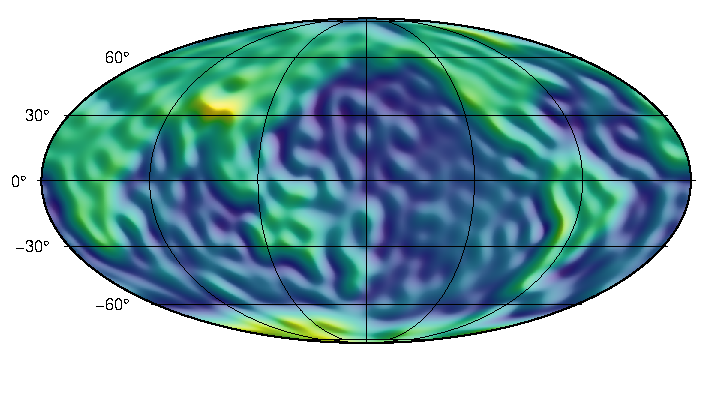
\includegraphics{./fig-h-shs-nmax30.pdf}
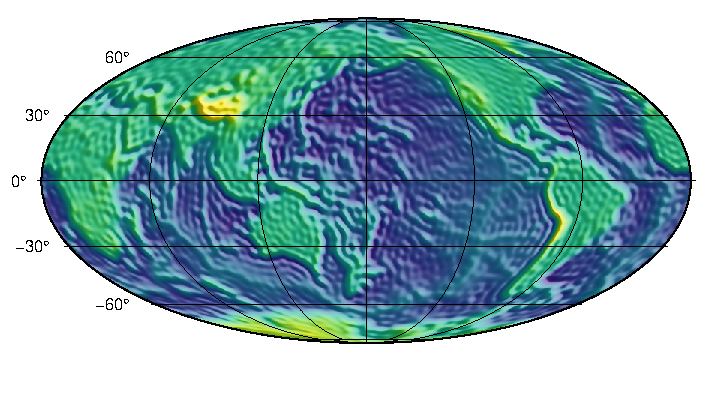
\includegraphics{./fig-h-shs-nmax90.pdf}
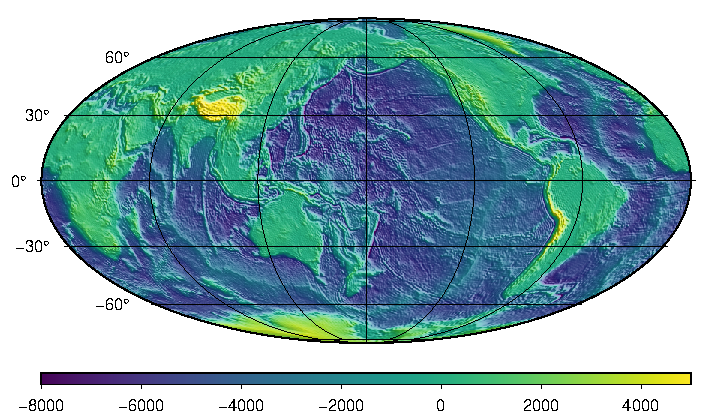
\includegraphics{./fig-h-shs-nmax360.pdf}
\caption{Sférický harmonický rozvoj zemskej topografie (jednotky~m) do 
stupňov~$N = 30$ (vrchná mapa), $90$~ (prostredná mapa) a~$360$~(spodná mapa).  
Výpočet bol uskutočnený Zdrojovým kódom~\ref{src:h_shs} 
z~Prílohy~\ref{app:shs_topography}.} \label{fig:shs_h}
\end{figure}

Okrem modelu~DTM2006.0 je voľne prístupný aj model Earth2014 
\parencite{Hirt2015}.  Earth2014 je kolekcia modelov zemskej topografie 
v~rozličných variantoch, napríklad so zohľadnením výšky ľadovcov či s~uvážením 
alebo bez uváženia batymetrie.  Model DTM2006.0 je dostupný do stupňa~$2190$.  
Maximálny stupeň modelu Earth2014 je~$10\, 800$.

Zo sférických harmonických modelov topografie nebeských telies spomeňme aspoň 
model topografie zemského Mesiaca do stupňa~2600, MoonTopo2600pa.shape 
\parencite{Wieczorek2015}, a~model tvaru asteroidu~Eros do stupňa~24 
\parencite{Zuber2000}.





% -----------------------------------------------------------------------------

\section{Konvergencia sférického harmonického rozvoja na povrchu Zeme}
\label{sec:convergence_of_spherical_harmonics}

Pred rozvinutím generickej funkcie pre Legendreove polynómy do Maclaurinovho 
radu (vzťah~\ref{eq:maclaurin_series_of_generic_function}) sme vyslovili 
predpoklad $\frac{r_Q}{r} < 1$.  Bez splnenia tejto podmienky 
rad~(\ref{eq:maclaurin_series_of_generic_function}) nemusí konvergovať.  
V~takom prípade nie je možné pokračovať v~odvodení 
z~Kapitoly~\ref{sec:vg_sh_expansion}.  Ak totiž 
rad~(\ref{eq:maclaurin_series_of_generic_function}) diverguje, zámena poradia 
integrácie a~sumácie nie je možná.  Na získanie vzťahu~(\ref{eq:vg_sh_no_norm}) 
sme preto museli predpokladať, že podmienka $\frac{r_Q}{r} < 1$ je splnená.

\begin{figure}
\centering
\input{./fig-spherical-harmonics-convergence.pdf_tex}
\caption{Sférický harmonický rad~(\ref{eq:vg_sh_no_norm}) konverguje rovnomerne 
a~absolútne vo vonkajšom priestore sféry konvergencie.  Svetlosivá farba 
označuje oblasť, v~ktorej nie je zaručená konvergencia.  Tmavosivá farba 
predstavuje hmoty telesa, ktoré generuje gravitačné pole.  V~tejto oblasti 
rad~(\ref{eq:vg_sh_no_norm}) nepopisuje skutočný gravitačný potenciál.}
\label{fig:spherical_harmonics_convergence}
\end{figure}

Nerovnosť $\frac{r_Q}{r} < 1$ môžeme prepísať do tvaru $r > r_Q$.  Táto
nerovnosť je splnená pre \emph{všetky} diferenciálne elementy $\diff \tau(r_Q,
\varphi_Q, \lambda_Q)$ iba vtedy, ak pre sprievodič $r$ výpočtového bodu $P(r,
\varphi, \lambda)$ platí
%
\begin{equation}
\label{eq:spherical_harmonic_convergence}
r > \max(r_Q) = R{,}
\end{equation}
%
kde $R$ je sprievodič najvzdialenejšieho diferenciálneho elementu $\diff\tau$ 
od začiatku súradnicového systému.  Sféra s~polomerom $R$ sa nazýva sféra 
konvergencie \parencite{Hotine} 
(Obrázok~\ref{fig:spherical_harmonics_convergence}).  Vo vonkajšom priestore 
sféry konvergencie rad~(\ref{eq:vg_sh_no_norm}) konverguje rovnomerne 
a~absolútne.  Na tejto sfére ani v~jej vnútri konvergencia zaručená nie je.

Nanešťastie, celý povrch Zeme sa nachádza v~oblasti, v~ktorej sférický 
harmonický rozvoj gravitačného potenciálu nemusí konvergovať.  Našťastie, zdá 
sa, že otázka konvergencie, resp. divergencie radu~(\ref{eq:vg_sh_no_norm}) nie 
je v~súčasnosti z~praktického hľadiska relevantná pre nízke až stredné stupne 
a~svoju závažnosť nadobúda až približne od stupňa $10{,}800$ 
\parencite{Hirt2016,Rexer2017}.

Konvergencia radu sférických harmonických funkcií na povrchu Zeme je často 
diskutovanou témou geodetickej literatúry 
\parencite{Hotine,Borre_chapter4,MoritzAdvancedGeodesy,Sjoberg1980,Jekeli1983,SansoGeoidDetermination}.






% -----------------------------------------------------------------------------

\chapter{Sféroidický harmonický rozvoj}
\label{sec:spheroidal_harmonics_chapter}

V~niektorých situáciách je potrebné skúmať gravitačné pole sploštených telies, 
napríklad samotnej Zeme či mnohých asteroidov Slnečnej sústavy (napríklad Eros, 
Castalia či Bennu; pozri \cite{Garmier2001}, \cite{Hu2015}, \cite{Sebera2016} 
či \cite{Reimond2016}).  Ak by sme rozvinuli gravitačný potenciál týchto telies 
do radu sférických harmonických funkcií~(\ref{eq:vg_sh_no_norm}), oblasť 
potenciálnej divergencie môže byť pomerne rozsiahla (porovnaj 
Obrázky~\ref{fig:spherical_harmonics_convergence} 
a~\ref{fig:spheroidal_harmonics_convergence}).  V~takýchto prípadoch môže byť 
výhodnejšie nerozvíjať gravitačný potenciál do radu harmonických funkcií vo 
sférických súradniciach, ale v~súradniciach, ktoré sú akýmsi spôsobom 
prirodzenejšie pre sploštené telesá.  Príkladom takýchto súradníc sú 
\emph{redukované elipsoidické súradnice}, ktoré vedú ku \emph{sféroidickému 
harmonickému rozvoju} gravitačného potenciálu.  Výhodou sféroidického 
harmonického rozvoja je spravidla väčšia oblasť konvergencie harmonického radu 
v~porovnaní so sférickým rozvojom (pozri 
Obrázok~\ref{fig:spheroidal_harmonics_convergence}).

V~tejto kapitole popíšeme redukované elipsoidické súradnice 
(Kapitola~\ref{sec:reduced_ell_coords}), sféroidické harmonické funkcie 
(Kapitola~\ref{sec:spheroidal_harmonics}) a~rozvoj gravitačného potenciálu do 
sféroidického harmonického radu 
(Kapitola~\ref{sec:spheroidal_harmonic_expansion}).  Kvôli náročnosti nebudeme 
odvádzať sféroidické harmonické funkcie rovnako podrobne ako sme odvodili 
sférické harmonické funkcie v~Kapitole~\ref{sec:spherical_harmonic_expansion}.  
Namiesto toho sa budeme snažiť prirovnávať diskutované témy k~problematike 
známej už z~Kapitoly~\ref{sec:spherical_harmonic_expansion}.  Získané poznatky 
potom využijeme v~Kapitole~\ref{sec:normal_gravity_field}, v~ktorej je 
študované gravitačné a~tiažové pole s~konštantným tiažovým potenciálom na 
povrchu dvojosového elipsoidu.

\begin{figure}
\centering
\input{./fig-spheroidal-harmonics-convergence.pdf_tex}
\caption{Sféra a~elipsoid konvergencie harmonických 
radov~(\ref{eq:vg_sh_no_norm}) a~(\ref{eq:vg_spheroidalh_2nd_norm_ynk}).  Oba 
rady konvergujú vo vonkajšom priestore svojej plochy konvergencie, no v~jej 
vnútri ich konvergencia zaručená nie je.  Oblasť konvergencie sféroidického 
harmonického radu je tak väčšia o~vyšrafovanú oblasť.}
\label{fig:spheroidal_harmonics_convergence}
\end{figure}


\section{Redukované elipsoidické súradnice}
\label{sec:reduced_ell_coords}

Nech je daný dvojosový referenčný elipsoid s~dĺžkou hlavnej polosi $a$ 
a~s~dĺžkou vedľajšej polosi $b$.  Parametre~$a$ a~$b$ sú volené tak, aby vhodne 
aproximovali tvar telesa, napríklad v~zmysle metódy najmenších štvorcov.  
Zaveďme parameter \emph{lineárna excentricita}~$E$, ktorý bude označovať 
vzdialenosť medzi stredom elipsy, ktorá vznikne meridiánovým rezom elipsoidu 
a jedným z~jej ohnísk (Obrázok~\ref{fig:reduced_ell_coords}).  Z~definície 
elipsy vyplýva, že lineárna excentricita je daná vzťahom
%
\begin{equation}
\label{eq:linear_eccentricity}
E = \sqrt{a^2 - b^2}{.}
\end{equation}

Polohu ľubovoľného bodu~$P$, ktorý sa nachádza na referenčnom elipsoide alebo 
nad ním, možno vyjadriť pomocou redukovaných elipsoidických súradníc $u$, 
$\beta$ a~$\lambda$ (Obrázok~\ref{fig:reduced_ell_coords}).  Symbol $u$ 
označuje malú polos konfokálneho elipsoidu, ktorý prechádza bodom~$P$.  
\emph{Konfokálny elipsoid} je taký elipsoid, ktorý má rovnaký stred~$O$ 
a lineárnu excentricitu~$E$ ako referenčný elipsoid.  Ak sa bod~$P$ nachádza na 
referenčnom elipsoide, potom~$u = b$.  Symbol $\beta$ predstavuje redukovanú 
elipsoidickú šírku.  Redukovaná elipsoidická dĺžka $\lambda$ je definovaná 
rovnako ako v~prípade sférických súradníc (pozri Obrázok~\ref{fig:cart_sph}).

\begin{figure}
\centering
\input{./fig-reduced-ell-coords.pdf_tex}
\caption{Redukované elipsoidické súradnice $u$ a~$\beta$ bodu $P$ vyjadrené 
pomocou referenčného elipsoidu s~hlavnou polosou~$a$ a~vedľajšou polosou~$b$.}
\label{fig:reduced_ell_coords}
\end{figure}

Jednoduchým spôsobom možno overiť, že medzi redukovanými elipsoidickými 
súradnicami a~karteziánskymi súradnicami platia nasledovné vzťahy,
%
\begin{equation}
\label{eq:ellred2cart}
\begin{split}
x &= \sqrt{u^2 + E^2} \, \cos\beta \, \cos\lambda{,}\\
y &= \sqrt{u^2 + E^2} \, \cos\beta \, \sin\lambda{,}\\
z &= u \, \sin\beta{,}
\end{split}
\end{equation}
%
kde $\sqrt{u^2 + E^2}$ je dĺžka hlavnej polosi konfokálneho elipsoidu.  Ak $E 
= 0$, teda ak referenčný elipsoid nie je sploštený, potom 
vzťah~(\ref{eq:ellred2cart}) má rovnaký tvar ako transformácia sférických 
súradníc na karteziánske súradnice~(\ref{eq:sph2cart}).



\subsection{Operátor gradient a~Laplaceova rovnica v~redukovaných 
elipsoidických súradniciach}
\label{sec:gradient_and_laplace_in_reduced_ell_coords}

Z~podobných dôvodov ako v~Kapitole~\ref{sec:laplace_equation_sph} potrebujeme 
vyjadriť operátor gradient a~Laplaceov operátor aj v~systéme redukovaných 
elipsoidických súradníc.  Príslušné vzťahy nájdeme postupom uvedeným 
v~Prílohách~\ref{app:gradient_in_orthogonal_coordinates} 
a~\ref{app:laplace_in_orthogonal_coordinates}.

V~súlade s~Prílohou~\ref{app:gradient_in_orthogonal_coordinates} definujme 
vektory (pozri vzťah~\ref{eq:xi1xi2xi3_vectors})
%
\begin{equation}
\label{eq:eu_ebeta_elon}
\hat{\vec e}_1^\mathrm{r} = \frac{\partial \vec r(\beta, \lambda, u)}{\partial 
\beta}{,}
%
\quad
%
\hat{\vec e}_2^\mathrm{r} = \frac{\partial \vec r(\beta, \lambda, u)}{\partial 
\lambda}{,}
%
\quad
%
\hat{\vec e}_3^\mathrm{r} = \frac{\partial \vec r(\beta, \lambda, u)}{\partial 
u}{,}
%
\end{equation}
%
kde
%
\begin{equation}
\vec r =
%
\begin{bmatrix}
x(\beta, \lambda, u)\\
y(\beta, \lambda, u)\\
z(\beta, u)
\end{bmatrix}
{,}
%
\end{equation}
%
pričom funkcie $x(\beta, \lambda, u)$, $y(\beta, \lambda, u)$ a~$z(\beta, u)$ 
sú dané vzťahmi~(\ref{eq:ellred2cart}).  Začiatok a~smery vektorov~$\hat{\vec 
e}_i^\mathrm{r}$, $i = 1, 2, 3$, definujú lokálny karteziánsky súradnicový 
systém~$x^\mathrm{r}$, $y^\mathrm{r}$, $z^\mathrm{r}$ s~pohyblivým 
začiatkom~v~bode~$P$.  Os~$z^\mathrm{r}$ je daná smerom vonkajšej normály ku 
konfokálnemu elipsoidu v~bode~$P$.  Os~$x^\mathrm{r}$ leží v~dotykovej rovine 
ku konfokálnemu elipsoidu a~smeruje na sever.  Os~$y^\mathrm{r}$ dotvára 
pravouhlý \emph{ľavotočivý} súradnicový systém.
%
Pomocou rovníc~(\ref{eq:ellred2cart}) a~(\ref{eq:eu_ebeta_elon}) možno 
jednoducho ukázať, že pre $\| \hat{\vec e}_i^\mathrm{r} \|$, $i = 1, 2, 3$, 
platí
%
\begin{equation}
\label{eq:ei_reduced_ell_magnitudes}
\begin{split}
\| \hat{\vec e}_1^\mathrm{r} \| &= \sqrt{u^2 + E^2 \, \sin^2\beta}{,}\\
%
\| \hat{\vec e}_2^\mathrm{r} \| &= \sqrt{\left( u^2 + E^2 \right)} \, 
\cos\beta{,}\\
%
\| \hat{\vec e}_3^\mathrm{r} \| &= \sqrt{\frac{u^2 + E^2 \, \sin^2\beta}{u^2 
+ E^2}}{.}
\end{split}
\end{equation}

Kombináciou rovníc~(\ref{eq:grad_orthogonal_system}) 
a~(\ref{eq:ei_reduced_ell_magnitudes}) získame operátor gradient v~redukovaných 
elipsoidických súradniciach,
%
\begin{align}
\label{eq:gradient_red_ell}
\nabla = \grad &= \vec e_1^\mathrm{r} \, \frac{1}{\sqrt{u^2 + E^2 \, 
\sin^2\beta}} \, \frac{\partial}{\partial \beta} + \vec e_2^\mathrm{r} \, 
\frac{1}{\sqrt{u^2 + E^2} \, \cos\beta} \, \frac{\partial}{\partial \lambda} 
+ \vec e_3^\mathrm{r} \, \sqrt{\frac{u^2 + E^2}{u^2 + E^2 \, \sin^2\beta}} \, 
\frac{\partial}{\partial u}\nonumber\displaybreak[2]\\
%
&=
%
\begin{bmatrix}
\dfrac{1}{\sqrt{u^2 + E^2 \, \sin^2\beta}} \, \dfrac{\partial}{\partial 
\beta}\\[2ex]
\dfrac{1}{\sqrt{u^2 + E^2} \, \cos\beta} \, \dfrac{\partial}{\partial 
\lambda}\\[2ex]
\sqrt{\dfrac{u^2 + E^2}{u^2 + E^2 \, \sin^2\beta}} \, \dfrac{\partial}{\partial 
u}
\end{bmatrix}
{,}
\end{align}
%
kde
%
\begin{equation}
\vec e_i^\mathrm{r} = \frac{\hat{\vec e}_i^\mathrm{r}}{\| \hat{\vec 
e}_i^\mathrm{r} \|}{,} \quad i = 1, 2, 3{,}
\end{equation}
%
sú jednotkové vektory v~smere osí~$x^\mathrm{r}$, $y^\mathrm{r}$ 
a~$z^\mathrm{r}$.

Laplaceovu rovnicu pre gravitačný potenciál dostaneme pomocou 
vzťahov~(\ref{eq:ei_reduced_ell_magnitudes}) 
a~(\ref{eq:laplace_orthogonal_system_final_2})
\parencite{MoritzPhysicalGeodesy},
%
\begin{equation}
\label{eq:vg_laplace_ellred}
(u^2 + E^2) \, \frac{\partial^2 V_\gidx}{\partial u^2} + 2u \, \frac{\partial 
V_\gidx}{\partial u} + \frac{1}{\cos\beta} \, \frac{\partial}{\partial\beta} 
\left( \cos\beta \, \frac{\partial V_\gidx}{\partial\beta} \right) + \frac{u^2 
+ E^2 \, \sin^2\beta}{(u^2 + E^2) \, \cos^2\beta} \, \frac{\partial^2 
V_\gidx}{\partial \lambda^2} = 0{.}
\end{equation}



\section{Sféroidické harmonické funkcie}
\label{sec:spheroidal_harmonics}

V~Kapitole~\ref{sec:vg_sh_expansion} sme uviedli, že k~rozvoju gravitačného 
potenciálu do radu sférických harmonických funkcií~(rovnica 
\ref{eq:vg_sh_no_norm}) je možné dopracovať sa aj riešením Laplaceovej 
diferenciálnej rovnice metódou separácie premenných vo sférických 
súradniciach~(rovnica~\ref{eq:vg_laplace_sph}).  Cieľom takéhoto prístupu je 
nájsť tri funkcie, $f_{\mathrm{s}}(r)$, $g_{\mathrm{s}}(\varphi)$ 
a $h_{\mathrm{s}}(\lambda)$.  Je možne ukázať, že riešením tejto úlohy sú 
funkcie nasledovného tvaru (porovnaj s~rovnicou~\ref{eq:vg_sh_no_norm}),
%
\begin{align}
\label{eq:fs}
f_{\mathrm{s}}(r) &= \dfrac{1}{r^{n + 1}}{,}\\
%
\label{eq:gs}
g_{\mathrm{s}}(\varphi) &= P_{nm}(\sin\varphi){,}\\
%
\label{eq:hs}
h_{\mathrm{s}}(\lambda) &=
%
\begin{cases}
\cos(m\,\lambda){,}\\
\sin(m\,\lambda){,}
\end{cases}
\end{align}
%
kde $n = 0, 1, 2, \dots$ a~$m = 0, 1, \dots, n$.  Pre úplnosť dodajme, že 
funkcia $f_{\mathrm{s}}(r)$ môže mať aj tvar $f_{\mathrm{s}}(r) = r^n$.  Toto 
riešenie sa využíva na rozvoj \emph{harmonickej} funkcie vo vnútri sféry 
\parencite{MoritzPhysicalGeodesy}.  Takáto situácia ale nie je predmetom tejto 
práce.

Jeden z~možných prístupov získania sféroidických harmonických funkcií je práve 
riešením Laplaceovej diferenciálnej rovnice v~redukovaných elipsoidických 
súradniciach~(\ref{eq:vg_laplace_ellred}) metódou separácie premenných.  Týmto 
spôsobom získame funkcie \parencite{MoritzPhysicalGeodesy}
%
\begin{align}
\label{eq:fr}
f_{\mathrm{r}}(u) &=
Q_{nm}\left( i \dfrac{u}{E} \right){,}\\
%
\label{eq:gr}
g_{\mathrm{r}}(\beta) &= P_{nm}(\sin\beta){,}\\
%
\label{eq:hr}
h_{\mathrm{r}}(\lambda) &=
%
\begin{cases}
\cos(m\,\lambda){,}\\
\sin(m\,\lambda){,}
\end{cases}
\end{align}
%
kde $i^2 = -1$ je imaginárna jednotka.  Podobne ako v~rovnici~(\ref{eq:fs}), 
funkcia~$f_{\mathrm{r}}(u)$ môže mať ďalší tvar $f_{\mathrm{r}}(u) 
= P_{nm}\left( i \frac{u}{E} \right)$, ktorý sa využíva na rozvoj 
\emph{harmonickej} funkcie vo vnútri referenčného elipsoidu.

Člen $Q_{nm}\left( i \frac{u}{E} \right)$ v~rovnici~(\ref{eq:fr}) sa nazýva 
\emph{pridružená Legendreova funkcia druhého druhu}.  Pre komplexný argument $z 
= i \frac{u}{E}$ je definovaná vzťahom \parencite{MoritzPhysicalGeodesy}
%
\begin{equation}
\label{eq:qnm_imag_def}
Q_{nm}(z) = (z^2 - 1)^{m \slash 2} \, \frac{\diff^m Q_n(z)}{\diff z^m}{,}
\end{equation}
%
kde
%
\begin{equation}
\label{eq:qn0_imag_def}
Q_{n}(z) = \frac{1}{2} \, P_n(z) \, \ln\frac{z + 1}{z - 1} - \sum_{s = 1}^n 
\frac{1}{s} \, P_{s - 1}(z) \, P_{n - s}(z){.}
\end{equation}
%
Pre reálny argument $t$ je definovaná vzťahom\footnote{V~niektorej literatúre 
sú Legendreove funkcie druhého druhu reálneho argumentu definované aj 
s~použitím Condonovho--Shortleyho fázového faktora $(-1)^m$ (pozri 
Kapitolu~\ref{sec:legendre_functions_cs_factor} a~napríklad \cite{Olver2010}).}
\parencite{MoritzPhysicalGeodesy}
%
\begin{equation}
\label{eq:qnm_real_def}
Q_{nm}(t) = (1 - t^2)^{m \slash 2} \, \frac{\diff^m Q_n(t)}{\diff t^m}{,}
\end{equation}
%
kde
%
\begin{equation}
\label{eq:qn0_real_def}
Q_{n}(t) = \frac{1}{2} \, P_n(t) \, \ln\frac{1 + t}{1 - t} - \sum_{s = 1}^n 
\frac{1}{s} \, P_{s - 1}(t) \, P_{n - s}(t){.}
\end{equation}

\begin{figure}
\centering
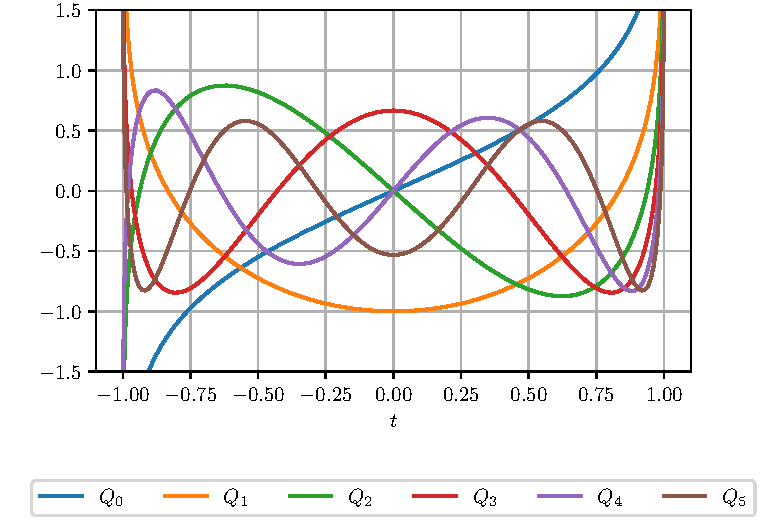
\includegraphics{./fig-legendre-polynomials-qn.pdf}
\caption{Legendreove polynómy druhého druhu reálneho argumentu $t$.}
\label{fig:lp_2nd}
\end{figure}

\begin{figure}
\centering
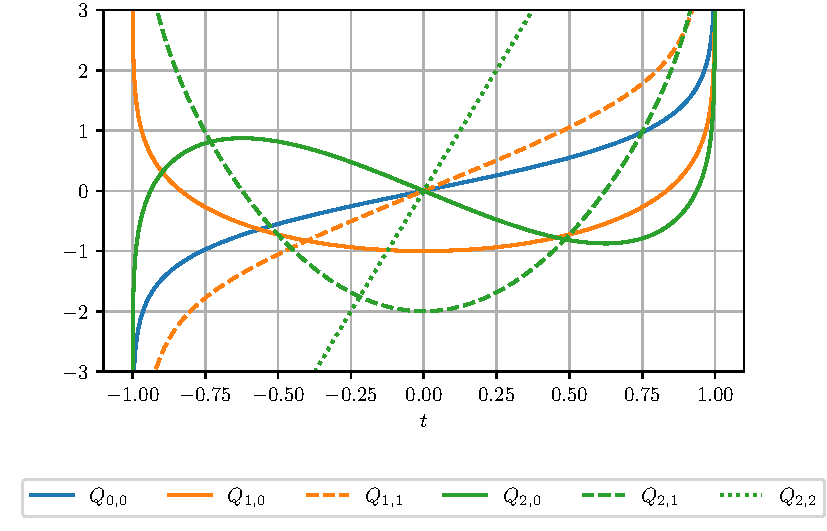
\includegraphics{./fig-legendre-functions-qnm.pdf}
\caption{Legendreove funkcie druhého druhu reálneho argumentu $t$.}
\label{fig:lf_2nd}
\end{figure}

Rovnica~(\ref{eq:qnm_real_def}) je formálne podobná rovnici~(\ref{eq:pnm_def}).  
Napriek tomu, v~dôsledku rozdielnej definície derivovaných členov~$Q_n(t)$ ide 
o~funkcie s~odlišným priebehom ako~$P_{nm}(t)$.  Uveďme pre názornosť 
explicitné vzťahy na výpočet funkcií~$Q_0\left( t \right)$, $Q_1\left( 
t \right)$ a~$Q_2\left( t \right)$ a~porovnajme ich 
s~rovnicami~(\ref{eq:p0_to_p5})
\parencite{MoritzPhysicalGeodesy},
%
\begin{align}
\label{eq:q0t}
Q_0(t) &= \frac{1}{2} \, \ln\frac{1 + t}{1 - t} = \mathrm{arctanh}(t){,}\\
%
\label{eq:q1t}
Q_1(t) &= \frac{t}{2} \, \ln\frac{1 + t}{1 - t} - 1 = t \, \mathrm{arctanh}(t)- 
 1{,}\\
%
\label{eq:q2t}
Q_2(t) &= \left( \frac{3}{4} t^2 - \frac{1}{4} \right) \, \ln\frac{1 + t}{1 
- t} - \frac{3}{2}t = \left( \frac{3}{2} t^2 - \frac{1}{2} \right) \, 
\mathrm{arctanh}(t) - \frac{3}{2}t{,}
\end{align}
%
kde
%
\begin{equation}
\label{eq:tanh}
\frac{1}{2} \, \ln \frac{1 + t}{1 - t} = \mathrm{arctanh} \, t{,}
\end{equation}
%
pričom $\mathrm{arctanh}$ označuje inverznú funkciu k~hyperbolickému tangensu, 
ktorý je daný vzťahom \parencite{Gradshteyn2007}
%
\begin{equation}
\tanh t = \frac{e^t - e^{-t}}{e^t + e^{-t}}{.}
\end{equation}
%
Funkcie $Q_{nm}(t)$ pre niekoľko prvých stupňov~$n$ a~rádov~$m$ sú znázornené 
na Obrázkoch~\ref{fig:lp_2nd} a~\ref{fig:lf_2nd} (porovnaj 
s Obrázkami~\ref{fig:lp} a~\ref{fig:lf}).  Funkcie $Q_0\left( z \right)$, 
$Q_1\left( z \right)$ a~$Q_2\left( z \right)$ komplexného argumentu~$z$ získame 
nahradením~výrazu~(\ref{eq:tanh}) vo vzťahoch~(\ref{eq:q0t}) až (\ref{eq:q2t}) 
výrazom (porovnaj rovnice~\ref{eq:qn0_imag_def} a~\ref{eq:qn0_real_def})
%
\begin{equation}
\label{eq:arccoth}
\frac{1}{2} \, \ln \frac{z + 1}{z - 1} = \mathrm{arccoth} \, z{,}
\end{equation}
%
kde $\mathrm{arccoth}$ je inverzná funkcia k hyperbolickému kotangensu, ktorý 
je daný vzťahom \parencite{Gradshteyn2007}
%
\begin{equation}
\coth z = \frac{1}{\tanh z} =  \frac{e^z + e^{-z}}{e^z - e^{-z}}{.}
\end{equation}

Pre~$Q_n(t)$ platia rovnaké rekurentné vzťahy ako pre~$P_n(t)$ 
\parencite{MoritzPhysicalGeodesy}.  Podobne ako funkcie $P_{nm}(t)$, i~funkcie 
$Q_{nm}(t)$ vyhovujú Legendreovej diferenciálnej rovnici druhého rádu 
\parencite[pozri rovnicu
\ref{eq:legfunc1_differential_equation};][]{MoritzPhysicalGeodesy}.  Všimnime 
si tiež, že pre $t \rightarrow \pm 1$, teda pre $\beta \rightarrow \pm 
\frac{\pi}{2}$, sa Legendreove funkcie druhého druhu blížia k~$\pm \infty$ 
(pozri rovnice~\ref{eq:qn0_imag_def} a~\ref{eq:qn0_real_def} 
a Obrázky~\ref{fig:lp_2nd} a~\ref{fig:lf_2nd}).  Túto vlastnosť budeme nazývať 
\emph{singularita}.  Práve kvôli singularite sa Legendreove funkcie druhého 
druhu nepoužívajú v~praktických aplikáciách ako riešenie pre funkcie 
$g_\mathrm{s}(\varphi)$ a~$g_\mathrm{r}(\beta)$ (pozri rovnice~\ref{eq:gs} 
a~\ref{eq:gr}), a~to napriek tomu, že sú taktiež riešením Legendreovej 
diferenciálnej rovnice \parencite{MoritzPhysicalGeodesy}.


\subsection{Numerický výpočet Legendreových funkcií druhého druhu}

Presný a~efektívny numerický výpočet funkcií $Q_{nm}\left( i \frac{u}{E} 
\right)$ je náročný, obzvlášť pre vysoké stupne a~rády.  Z~dôvodov, ktoré budú 
ozrejmené neskôr v~Kapitole~\ref{sec:spheroidal_harmonic_expansion}, sa 
v~praktických geodetických aplikáciách nezvyknú počítať členy $Q_{nm}\left( 
i \frac{u}{E} \right)$, ale iba podiely $Q_{nm}\left( i \frac{u}{E} \right) 
\slash Q_{nm}\left( i \frac{b}{E} \right)$.  Samotný výpočet, či už funkcií 
$Q_{nm}\left( i \frac{u}{E} \right)$ alebo podielov $Q_{nm}\left( i \frac{u}{E} 
\right) \slash Q_{nm}\left( i \frac{b}{E} \right)$, je zvyčajne uskutočňovaný 
rekurentnými vzťahmi alebo rozvojmi do nekonečných radov \parencite[pozri 
napríklad][]{Sebera2012,Fukushima2013,Wang2013,Sprlak2020}.



\section{Rozvoj gravitačného potenciálu do radu sféroidických harmonických 
funkcií}
\label{sec:spheroidal_harmonic_expansion}

Gravitačný potenciál v~bodoch mimo telesa môže byť rozvinutý do radu 
sféroidických harmonických funkcií vzťahom \parencite{MoritzPhysicalGeodesy}
%
\begin{equation}
\label{eq:vg_spheroidalh_2nd_norm_ynk}
V_\gidx(u, \beta, \lambda) = \frac{GM}{R} \, \sum_{n = 0}^\infty \sum_{k 
= -n}^n \frac{Q_{n|k|}\left( i \dfrac{u}{E} \right)}{Q_{n|k|}\left( 
i \dfrac{b}{E} \right)} \, \bar{v}^{\mathrm{r}}_{nk} \, \bar{Y}_{nk}(\beta, 
\lambda){,}
\end{equation}
%
kde $\bar{v}_{nk}^\mathrm{r}$ sú \emph{úplne normované sféroidické harmonické 
koeficienty} gravitačného potenciálu.  
Rovnica~(\ref{eq:vg_spheroidalh_2nd_norm_ynk}) je lineárnou kombináciou funkcií 
(\ref{eq:fr}), (\ref{eq:gr}) a~(\ref{eq:hr}) (pozri tiež 
vzťah~\ref{eq:ynk_norm}), ktoré boli získané riešením Laplaceovej 
diferenciálnej rovnice metódou separácie premenných v~redukovaných 
elipsoidických súradniciach.

Rovnica~(\ref{eq:vg_spheroidalh_2nd_norm_ynk}) je formálne podobná 
vzťahu~(\ref{eq:vg_sh_2nd_norm_ynk}).  Môže byť tiež jednoducho prepísaná do 
tvaru, ktorý využíva index~$m = 0, 1, \dots, n$ (porovnaj 
rovnice~\ref{eq:vg_sh_2nd_norm} a~\ref{eq:vg_sh_2nd_norm_ynk}) či do radu 
nenormovaných sféroidických harmonických funkcií, podobne ako je tomu 
v~rovniciach~(\ref{eq:vg_sh_no_norm}) a~(\ref{eq:vg_sh_1st_norm}),
%
\begin{equation}
\label{eq:vg_spheroidalh_no_norm}
V_\gidx(u, \beta, \lambda) = \sum_{n = 0}^\infty \sum_{m = 0}^n 
\frac{Q_{nm}\left( i \dfrac{u}{E} \right)}{Q_{nm}\left( i \dfrac{b}{E} \right)} 
\, \left( C^{\mathrm{r}}_{nm} \, \cos(m\lambda) + S^{\mathrm{r}}_{nm} \, 
\sin(m\lambda) \right) \, P_{nm}(\sin\beta){.}
\end{equation}
%
Funkcia $Q_{n|k|}\left( i \frac{u}{E} \right)$ zo vzťahu~(\ref{eq:fr}) je 
komplexná funkcia.  Vo sféroidických harmonických 
rozvojoch~(\ref{eq:vg_spheroidalh_2nd_norm_ynk}) 
a~(\ref{eq:vg_spheroidalh_no_norm}) je preto vydelená funkciou $Q_{n|k|}\left( 
i \frac{b}{E} \right)$ tak, aby výsledný podiel bol reálne číslo.  Tým je 
zabezpečené, že i~sféroidické harmonické koeficienty sú reálne čísla.  Všimnime 
si tiež, že pred prvou sumáciou vo vzťahu~(\ref{eq:vg_spheroidalh_no_norm}) sa 
nenachádza Newtonova gravitačná konštanta~$G$ tak, ako je tomu vo 
vzťahu~(\ref{eq:vg_sh_no_norm}).  Ide len konvenciu, konštanta~$G$ je tým pádom 
obsiahnutá vo sféroidických harmonických koeficientoch~$C_{nm}^\mathrm{r}$ 
a~$S_{nm}^\mathrm{r}$.  Rovnice~(\ref{eq:vg_spheroidalh_2nd_norm_ynk}) 
a~(\ref{eq:vg_spheroidalh_no_norm}) konvergujú vo vonkajšom priestore elipsoidu 
konvergencie (pozri Obrázok~\ref{fig:spheroidal_harmonics_convergence}).  Na 
povrchu elipsoidu konvergencie a/alebo v~neho vnútri konvergencia zaručená nie 
je.

Člen $Q_{n|k|}\left( i \frac{u}{E} \right) \slash Q_{n|k|}\left( i \frac{b}{E} 
\right)$ v~rovnici~(\ref{eq:vg_spheroidalh_2nd_norm_ynk}) má podobnú úlohu, akú 
má člen $\left( \frac{R}{r} \right)^{n + 1}$ 
vo~vzťahu~(\ref{eq:vg_sh_2nd_norm_ynk}), teda umožniť výpočet gravitačného 
potenciálu aj nad referenčným elipsoidom (v~prípade sférického harmonického 
rozvoja nad referenčnou sférou s~polomerom~$R$).  V~súvislosti 
s~rovnicou~(\ref{eq:ellred2cart}) sme uviedli, že pre~$E = 0$ sú redukované 
elipsoidické súradnice $u$, $\beta$ a~$\lambda$ totožné so sférickými 
súradnicami $r$, $\varphi$ a~$\lambda$.  Pre $E \rightarrow 0$ tiež platí vzťah 
\parencite{MoritzPhysicalGeodesy}
%
\begin{equation}
\lim_{E \rightarrow 0} \frac{Q_{n|k|}\left( i \dfrac{u}{E} 
\right)}{Q_{n|k|}\left( i \dfrac{b}{E} \right)} = \left( \frac{R}{r} \right)^{n 
+ 1}{.}
\end{equation}
%
Sférický harmonický rozvoj~(\ref{eq:vg_sh_2nd_norm_ynk}) preto možno považovať 
za špeciálny prípad zovšeobecneného sféroidického harmonického 
rozvoja~(\ref{eq:vg_spheroidalh_2nd_norm_ynk}).

Na záver dodajme, že Laplaceovu rovnicu možno riešiť aj v~súradnicovom systéme, 
ktorý je vztiahnutý k~trojosovému elipsoidu s~polosami $a$, $b$, $c$.  Získame 
tým rozvoj gravitačného potenciálu do radu elipsoidických harmonických funkcií 
\parencite[napríklad][]{Garmier2001,Hu2015,Reimond2016}.  Tento prístup je 
zložitejší ako sférické a~sféroidické harmonické rozvoje a~vo fyzikálnej 
geodézii sa využíva zriedka.  Uplatnenie má najmä v~súvislosti s~modelovaním 
gravitačného poľa v~blízkosti asteroidov, ktoré majú komplikovaný tvar.








% -----------------------------------------------------------------------------


\chapter{Normálne tiažové pole}
\label{sec:normal_gravity_field}

Fyzikálna geodézia určuje tvar Zeme z~informácie o~jej tiažovom poli, napríklad 
z~tiažového potenciálu a~z~vektora tiažového zrýchlenia na povrchu Zeme.  Táto 
úloha je neľahká, pretože vzťah medzi tiažovým poľom a~hľadaným zemským 
povrchom je nelineárny.  Spravidla sa preto pristupuje k~linearizácii pomocou 
rozvoja do Taylorovho radu, v~ktorom sa zanedbajú členy druhého a~vyšších 
rádov.  \emph{Normálne tiažové pole Zeme} je jednoduchý a~súčasne dostatočne 
presný model skutočného tiažového poľa Zeme, využívaný práve na výpočet 
približných hodnôt v~linearizovaných úlohách fyzikálnej geodézie.  Požiadavka 
jednoduchosti je odôvodnená potrebou prijateľne náročných výpočtov v~normálnom 
poli, napríklad pomocou uzavretých vzťahov pre \emph{normálne tiažové 
zrýchlenie} $\boldsymbol{\gamma}$ či \emph{normálny tiažový potenciál} $U$.  
Dostatočná presnosť je potrebná nato, aby bolo možné s~rozumnou mierou 
aproximácie zanedbať nelineárne členy Taylorovho rozvoja.  Požiadavky 
jednoduchosti a~presnosti normálneho tiažového poľa si vzájomne odporujú, preto 
je potrebné nájsť medzi nimi vhodný kompromis.

\section{Voľba normálneho tiažového poľa}
\label{sec:choice_of_normal_gravity_field}

Jedno z~najjednoduchších telies ponúkajúcich sa na definíciu normálneho 
tiažového poľa Zeme je \emph{homogénna rotujúca guľa} definovaná troma 
nezávislými parametrami.  Obvyklou trojicou nezávislých parametrov sú 
geocentrická gravitačná konštanta~$GM$, teda súčin Newtonovej gravitačnej 
konštanty~$G$ a~hmotnosti Zeme~$M$, ďalej polomer gule~$R$ a~uhlová rýchlosť 
rotácie~$\omega$.  Vonkajšie tiažové pole homogénnej gule je síce jednoducho 
matematicky opísateľné, nevyhovuje ale väčšine súčasných aplikácií z~hľadiska 
presnosti.  Vo fyzikálnej geodézii sa zvykne preto využívať prevažne len 
v~niektorých špecifických situáciách, napríklad ak postačuje i~nižšia presnosť.

V dôsledku sploštenia Zeme je dvojosový rotačný elipsoid presnejšou 
geometrickou aproximáciou geoidu ako sféra.  Okrem svojho geometrického tvaru 
je geoid špecifický tým, že hodnota skutočného tiažového potenciálu $W_0$ je 
konštantná v~každom jeho bode (pozri Kapitolu~\ref{sec:equipotential_surface}).  
Túto vlastnosť by bolo výhodné zužitkovať aj pri voľbe normálneho tiažového 
poľa, ktoré je založené na elipsoide.  Budeme preto požadovať, aby 
\emph{normálny tiažový potenciál} $U_0$ bol na povrchu elipsoidu konštantný.  
Vhodnou voľbou geometrických parametrov (napríklad hlavná a~vedľajšia polos) 
a fyzikálnych parametrov (napríklad normálny tiažový potenciál $U_0$) potom 
získame vernú aproximáciu geoidu, alebo inými slovami, dostatočne presné 
približné hodnoty na linearizáciu úloh, ktoré sú spojené s~určovaním geoidu.  
Dvojosový rotačný elipsoid s~konštantným normálnym tiažovým potenciálom na 
svojom povrchu sa nazýva \emph{ekvipotenciálny elipsoid}.  V~súčasnosti je to 
najčastejší spôsob voľby normálneho tiažového poľa Zeme.

Ďalšou možnosťou voľby normálneho tiažového poľa je sférický harmonický rozvoj 
gravitačného potenciálu do konečného harmonického stupňa 
(rovnice~\ref{eq:vg_sh_no_norm}, \ref{eq:vg_sh_1st_norm}, 
\ref{eq:vg_sh_2nd_norm} a~\ref{eq:vg_sh_2nd_norm_ynk}).  Plocha, na ktorej je 
takto definovaný normálny tiažový potenciál konštantný, sa nazýva 
\emph{sféroid}.  Obmedzením rozvoja potenciálu na stupeň~2 získame 
\emph{Brunsov sféroid} a~obmedzením na stupeň~4 získame \emph{Helmertov 
sféroid} \parencite{Moritz1967}.  V~oboch prípadoch sú koeficienty stupňa~1 
nulové, pretože začiatok súradnicového systému je vložený do ťažiska Zeme 
(pozri~Kapitolu~\ref{sec:physical_meaning_of_spherical_harmonic_coefficients}).  
V definícii Helmertovho sféroidu sú nulové navyše aj koeficienty stupňa~3 
z dôvodu zabezpečenia symetrie voči rovine rovníka (pozri geometrickú 
interpretáciu sférických harmonických funkcií 
v~Kapitole~\ref{sec:spherical_harmonics}).   V~praktických aplikáciách sa  
Brunsov ani Helmertov sféroid nezvyknú v~súčasnosti používať.  Obe plochy sú 
totiž veľmi blízke dvojosovému rotačnému elipsoidu, avšak sú výrazne 
zložitejšie.  Navyše, získaná dodatočná presnosť zväčša nie je významná 
\parencite{Moritz1967}.

Či už ide o~ekvipotenciálny elipsoid alebo sféroid, všimnime si, že v~ani 
jednom prípade sme nepotrebovali vysloviť predpoklad o~priestorovom rozložení 
hustôt.  Fyzikálna geodézia využíva normálne tiažové pole predovšetkým na účely 
linearizácie.  Zdá sa byť preto kľúčové najmä to, aby normálna ekvipotenciálna 
plocha s~normálnym tiažovým potenciálom~$U_0$ bola geometricky blízka geoidu, 
ďalej aby normálny tiažový potenciál~$U_0$ bol blízky skutočnému tiažovému 
potenciálu~$W_0$ na geoide, a~nakoniec aby geometrická aj fyzikálna časť 
normálneho poľa boli jednoducho matematicky opísateľné.  Pre niektoré príbuzné 
vedné odbory, napríklad geofyziku, je však znalosť hustoty v~normálnom telese 
potrebná \parencite{Karcol2017}.  V~takýchto situáciách nemusí byť voľba 
ekvipotenciálneho elipsoidu tá najvýhodnejšia.  Diskusiu k~možnostiam 
priestorového rozloženia hustoty vo vnútri ekvipotenciálneho elipsoidu je možné 
nájsť napríklad v~prácach \textcite{MoritzTheFigureOfTheEarth}, 
\textcite{TorgeGeodesy}, \textcite{Conway2000} či \textcite{Karcol2017}.



\section{Ekvipotenciálny elipsoid}
\label{sec:equipotential_ellipsoid}

Nech teleso s~hmotnosťou~$M$ rotuje konštantnou uhlovou rýchlosťou~$\omega$ 
okolo pevnej osi.  Nech $S$ je ekvipotenciálna plocha jeho tiažového poľa 
obklopujúca celé teleso.  \emph{Stokesov--Poincarého} teorém hovorí, že tiažový 
potenciál vo vonkajšom priestore plochy~$S$ je jednoznačne určený konštantami 
$M$ a~$\omega$ a~parametrami, ktoré definujú plochu~$S$ 
\parencite{TorgeGeodesy}.  G.~G.~Stokes (1819~-- 1903) bol írsko--anglický 
matematik a fyzik, ktorý významne prispel do viacerých vedných odvetví, 
napríklad do mechaniky tekutín (Navierova--Stokesova rovnica) či do optiky 
(polarizácia svetla).  H.~Poincaré (1854~-- 1912) bol francúzsky matematik 
a~teoretický fyzik.  V~geodézii je známy napríklad pre redukciu odmeraného 
tiažového zrýchlenia z~povrchu Zeme do vnútra Zeme \parencite[Poincaré--Prey 
redukcia, pozri napríklad][]{MoritzPhysicalGeodesy}.

Na jednoznačné definovanie ekvipotenciálneho elipsoidu a~jeho vonkajšieho 
tiažového poľa teda postačuje určiť štyri nezávislé \emph{základné parametre}.  
Dva z~týchto parametrov sú geometrické, resp. veľmi úzko súvisia s~geometriou 
elipsoidu (napríklad hlavná polos a~sploštenie elipsoidu), a~dva parametre sú 
fyzikálne (hmotnosť a~uhlová rýchlosť rotácie).  Všetky ostatné veličiny 
normálneho tiažového poľa je možné vypočítať z~týchto základných parametrov, či 
už ide o~geometrické parametre (napríklad vedľajšia polos či lineárna 
excentricita elipsoidu) alebo fyzikálne parametre (normálny tiažový potenciál 
a pod.).  Parametre, ktoré sú vypočítané zo základných parametrov, budeme 
nazývať \emph{odvodené parametre}.  Teóriu ekvipotenciálneho elipsoidu 
rozpracovali taliansky geodet, astronóm, geofyzik a~matematik P.~Pizzetti 
(1860--1918) a~taliansky matematik a~matematický fyzik C.~Somigliana 
(1860--1955) v~prácach \textcite{Pizzetti1984} a~\textcite{Somigliana1929}.

Základné parametre ekvipotenciálnych elipsoidov sú v~súčasnosti určované 
spravidla družicovými technikami a~astronomickými meraniami.  Historický 
prehľad geodetických referenčných systémov a~spôsoby ich určenia je možné nájsť 
napríklad v~prácach \textcite{TorgeGeodesy} a~\textcite{MoritzPhysicalGeodesy}.  
V ďalších častiach práce popíšeme dva najpoužívanejšie ekvipotenciálne 
elipsoidy (Kapitoly~\ref{sec:grs80} a~\ref{sec:wgs84}).  Následne odvodíme 
vzťahy na výpočet normálneho tiažového potenciálu pomocou rozvoja do radu 
sféroidických a~sférických harmonických 
funkcií~(Kapitola~\ref{sec:normal_gravity_potential}).  Na záver opíšeme spôsob 
výpočtu normálneho tiažového zrýchlenia (Kapitola~\ref{sec:normal_gravity}).  
Tieto poznatky budú dôležité neskôr v~Kapitole~\ref{sec:geoid}, ktorá sa 
zaoberá určovaním geoidu.  Po celý čas je pritom vhodné mať na pamäti, že 
normálne tiažové pole Zeme je matematicko-fyzikálny model, ktorý je definovaný 
štyrmi základnými parametrami.  Všetky ostatné parametre, či už geometrické 
alebo fyzikálne, sú odvoditeľné z~týchto parametrov.  S~výnimkou štyroch 
základných parametrov sa teda všetky veličiny normálneho tiažového poľa 
získavajú výpočtom, nie meraním ako je tomu v~prípade \emph{skutočného} 
tiažového poľa Zeme.





\subsection{Ekvipotenciálny elipsoid GRS80}
\label{sec:grs80}

Jednu z~možných štvoríc základných parametrov tvorí
%
\begin{itemize}
\item hlavná polos~$a$,
%
\item dynamický koeficient~$J_{2,0}$,
%
\item geocentrická gravitačná konštanta~$GM$~a
%
\item uhlová rýchlosť rotácie $\omega$.
\end{itemize}
%
Týmto základnými parametrami je definovaný ekvipotenciálny elipsoid 
\emph{GRS80} \parencite[angl. \textit{Geodetic Reference 
System~1980};][]{GRS80}.  Základné parametre GRS80 
(Tabuľka~\ref{tab:grs80_fundamental}) boli prijaté Medzinárodnou úniou geodézie 
a geofyziky (angl.~\textit{International Union of Geodesy and Geophysics}, 
IUGG) a~Medzinárodnou asociáciou geodézie IAG na 17.~generálnom zasadnutí IUGG 
v Canberra v~decembri 1979.

Všimnime si, že medzi základnými parametrami sa nachádza geocentrická 
gravitačná konštanta $GM$ a~nie hmotnosť Zeme~$M$, ktorá je podľa 
Stokesovho--Poincarého teorému postačujúca na jednoznačné definovanie tiažového 
potenciálu vo vonkajšom priestore ekvipotenciálnej plochy 
(Kapitola~\ref{sec:equipotential_ellipsoid}).  Dôvod je ten, že 
súčin~konštánt~$G$ a~$M$ je možné určiť presnejšie ako samostatný parameter~$M$ 
\parencite[pozri napríklad][]{Pick2000}.  Spomeňme tiež, že hodnota konštanty 
$GM$ z~Tabuľky~\ref{tab:grs80_fundamental} zahŕňa hmotnosť Zeme \emph{a} 
hmotnosť zemskej atmosféry a~koeficient $J_{2,0}$ nezahŕňa účinok permanentnej 
slapovej deformácie Zeme.  Medzi koeficientmi $J_{2,0}$ 
(Tabuľka~\ref{tab:grs80_fundamental}), $C_{2,0}$ 
(rovnica~\ref{eq:vg_sh_no_norm}) a~$\bar{C}_{2,0}$ 
(rovnica~\ref{eq:vg_sh_2nd_norm}) platia nasledovné vzťahy 
\parencite{Moritz1967,MoritzPhysicalGeodesy},
%
\begin{align}
\label{eq:c20_j20}
C_{2,0} &= -J_{2,0}{,}\\
%
\label{eq:c20_j20_2}
\bar{C}_{2,0} &= \frac{C_{2,0}}{\sqrt{5}} = -\frac{J_{2,0}}{\sqrt{5}}{.}
\end{align}

Tabuľka~\ref{tab:grs80_derived} uvádza číselné hodnoty niektorých odvodených geometrických 
a fyzikálnych parametrov ekvipotenciálneho elipsoidu~GRS80.  Medzi geometrické 
parametre sme zahrnuli, okrem iných, \emph{prvú numerickú excentricitu}
%
\begin{equation}
\label{eq:1st_eccentricity}
e = \frac{a^2 - b^2}{a} = \frac{E}{a}{,}
\end{equation}
%
\emph{druhú numerickú excentricitu}
%
\begin{equation}
\label{eq:2nd_eccentricity}
e' = \frac{a^2 - b^2}{b} = \frac{E}{b}{,}
\end{equation}
%
a \emph{sploštenie}
%
\begin{equation}
\label{eq:flattening}
f = \frac{a - b}{b}{.}
\end{equation}
%
Vzťahy na výpočet odvodených fyzikálnych parametrov z~Tabuľky~\ref{tab:grs80_derived} budú 
odvodené v~nasledujúcich častiach tejto kapitoly.

\begin{table*}
\begin{center}
\caption{Základné parametre ekvipotenciálneho elipsoidu GRS80.}
\label{tab:grs80_fundamental}
\small
\begin{tabular}{l l l l}
\hline
Označenie & Symbol & Jednotka & Popis\\
\hline
$a$       & $6\,378\,137$ & m & Hlavná polos\\
$J_{2,0}$ & $108\,263 \times 10^{-8}$ & Bezrozmerné & Dynamický faktor\\
$GM$ & $3\,986\,005 \times 10^8$ & $\mathrm{m}^3 \ \mathrm{s}^{-2}$ 
& Geocentrická gravitačná konštanta\\
$\omega$ & $7\,292\,115 \times 10^{-11}$ & $\mathrm{rad} \ \mathrm{s}^{-1}$ 
& Uhlová rýchlosť rotácie\\
\hline
\end{tabular}
\end{center}
\end{table*}

\begin{table*}
\begin{center}
\caption{Niektoré odvodené parametre ekvipotenciálneho elipsoidu GRS80 
\parencite{MoritzPhysicalGeodesy}.}
\label{tab:grs80_derived}
\small
\begin{tabular}{l l l l l}
\hline
Typ parametra & Symbol & Hodnota & Jednotka & Popis\\
\hline
Geometrický & $b$       & $6 \, 356 \, 752.3141$ & m & Vedľajšia polos\\
            & $E$       & $521 \, 854.0097$ & m & Lineárna excentricita\\
            & $e^2$     & $0.00669438002290$ & Bezrozmerné & Druhá mocnina 
            prvej\\
            &           &     &             & numerickej excentricity\\
            & $(e')^2$  & $0.00673949677548$ & Bezrozmerné & Druhá mocnina 
            druhej\\
            &           &     &             & numerickej excentricity\\
            & $f$       & $0.00335281068118$ & Bezrozmerné & Sploštenie\\
\hline
Fyzikálny & $U_0$       & $ 62 \, 636 \, 860.850$ & $\mathrm{m}^2 \, 
          \mathrm{s}^{-2}$ & Normálny tiažový\\
          &            &     &   & potenciál na elipsoide\\
          & $\gamma_a$ & $9.7803267715$ & $\mathrm{m} \, \mathrm{s}^{-2}$ 
& Normálne tiažové\\
          &            &     &   & zrýchlenie na rovníku\\
          & $\gamma_b$ & $9.8321863685$ & $\mathrm{m} \, \mathrm{s}^{-2}$ 
& Normálne tiažové\\
          &            &     &   & zrýchlenie na póle\\
          & $m$ & $0.00344978600308$ & Bezrozmerné & Pomocná konštanta,\\
          &     &                    &             & $m = \omega^2 \, a^2 \, 
b \slash (GM)$\\
\hline
\end{tabular}
\end{center}
\end{table*}

Elipsoid GRS80 je oficiálny referenčný systém Medzinárodnej asociácie geodézie.






\subsection{Ekvipotenciálny elipsoid WGS84}
\label{sec:wgs84}

Ďalšou možnosťou definície ekvipotenciálneho elipsoidu je použiť sploštenie~$f$ 
(rovnica~\ref{eq:flattening}) namiesto koeficientu~$J_{2,0}$.  Týmto spôsobom 
je definovaný ekvipotenciálny elipsoid \emph{WGS4} 
\parencite[angl. \textit{World Geodetic System~1984};][]{WGS84}, ktorý vychádza 
z~elipsoidu GRS80 (Tabuľka~\ref{tab:wgs84_fundamental}).  Vybraté odvodené 
parametre elipsoidu WGS84 sú uvedené v~Tabuľke~\ref{tab:wgs84_derived}.  
Z hľadiska tvaru sú oba elipsoidy podobné; dĺžka ich hlavnej polosi je $6\, 
378\, 137\ \mathrm{m}$ a~dĺžka vedľajšej polosi, vypočítaná zo základných 
parametrov, sa odlišuje iba o~desatinu milimetra (porovnaj 
Tabuľky~\ref{tab:grs80_derived} a~\ref{tab:wgs84_derived}).  Z~fyzikálneho 
hľadiska je už medzi elipsoidmi rozdiel väčší.  Uhlová rýchlosť rotácie oboch 
elipsoidov je síce rovnaká, no odlišné hodnoty geocentrických gravitačných 
konštánt spôsobujú rozdiel v~normálnom tiažovom potenciáli na elipsoide.  
Rozdiel medzi oboma hodnotami je približne o~5 rádov väčší ako v~súčasnosti 
dosiahnuteľná presnosť určenia rozdielu skutočného tiažového potenciálu medzi 
dvoma bodmi (pozri Kapitolu~\ref{sec:potential_differences}).

\begin{table*}
\begin{center}
\caption{Základné parametre ekvipotenciálneho elipsoidu WGS84 
\parencite{MoritzPhysicalGeodesy}.}
\label{tab:wgs84_fundamental}
\small
\begin{tabular}{l l l l}
\hline
Označenie & Symbol & Jednotka & Popis\\
\hline
$a$       & $6\,378\,137$ & m & Hlavná polos\\
$1 \slash f$ & $298.257223563$ & Bezrozmerné & Prevrátená hodnota sploštenia\\
$GM$ & $3\,986\,004.418 \times 10^8$ & $\mathrm{m}^3 \ \mathrm{s}^{-2}$ 
& Geocentrická gravitačná konštanta\\
$\omega$ & $7\,292\,115 \times 10^{-11}$ & $\mathrm{rad} \ \mathrm{s}^{-1}$ 
& Uhlová rýchlosť rotácie\\
\hline
\end{tabular}
\end{center}
\end{table*}

\begin{table*}
\begin{center}
\caption{Niektoré odvodené parametre ekvipotenciálneho elipsoidu WGS84 
\parencite{MoritzPhysicalGeodesy}.}
\label{tab:wgs84_derived}
\small
\begin{tabular}{l l l l l}
\hline
Typ parametra & Symbol & Hodnota & Jednotka & Popis\\
\hline
Geometrický & $b$       & $6 \, 356 \, 752.3142$ & m & Vedľajšia polos\\
            & $E$       & $521 \, 854.0084$ & m & Lineárna excentricita\\
            & $e^2$     & $0.00669437999014$ & Bezrozmerné & Druhá mocnina 
            prvej\\
            &           &     &             & numerickej excentricity\\
            & $(e')^2$  & $0.00673949674228$ & Bezrozmerné & Druhá mocnina 
            druhej\\
            &           &     &             & numerickej excentricity\\
            & $J_{2,0}$       & $108262.982131 \times 10^{-8}$ & Bezrozmerné 
& Dynamický faktor\\
\hline
Fyzikálny & $U_0$       & $ 62 \, 636 \, 851.715$ & $\mathrm{m}^2 \, 
          \mathrm{s}^{-2}$ & Normálny tiažový\\
          &            &     &   & potenciál na elipsoide\\
          & $\gamma_a$ & $9.7803253359$ & $\mathrm{m} \, \mathrm{s}^{-2}$ 
& Normálne tiažové\\
          &            &     &   & zrýchlenie na rovníku\\
          & $\gamma_b$ & $9.8321849378$ & $\mathrm{m} \, \mathrm{s}^{-2}$ 
& Normálne tiažové\\
          &            &     &   & zrýchlenie na póle\\
          & $m$ & $0.00344978650684$ & Bezrozmerné & Pomocná konštanta,\\
          &     &                    &             & $m = \omega^2 \, a^2 \, 
b \slash (GM)$\\
\hline
\end{tabular}
\end{center}
\end{table*}






\section{Normálny tiažový potenciál}
\label{sec:normal_gravity_potential}

V~mnohých situáciách, hoci rozhodne nie v~každej situácii, sú 
preferované~uzavreté matematické vzťahy pred nekonečnými rozvojmi.  Uzavretý 
vzťah je taký vzťah, ktorý má konečný počet členov.  Často umožňuje presnejší 
a rýchlejší číselný výpočet v~porovnaní s~príslušným nekonečným radom, pretože 
ten musí byť vždy obmedzený na vhodne zvolený konečný počet členov.  
V~Kapitole~\ref{sec:normal_gravity_potential_in_reduced_ell_coords} budeme 
preto hľadať uzavretý vzťah na výpočet normálneho tiažového potenciálu~$U$ 
v~bodoch na povrchu ekvipotenciálneho elipsoidu a~nad ním.  Pracovať budeme 
v~redukovaných elipsoidických súradniciach, ktoré sa prirodzene ponúkajú 
v~súvislosti so splošteným rotačným elipsoidom.  Následne 
v~Kapitole~\ref{sec:normal_gravity_potential_in_spherical_coords} vyjadríme 
normálny tiažový potenciál vo sférických súradniciach, tentokrát už ale pomocou 
nekonečného rozvoja.  
Kapitola~\ref{sec:normal_gravity_potential_in_reduced_ell_coords} je spracovaná 
podľa~\textcite{MoritzTheFigureOfTheEarth}.



\subsection{Normálny tiažový potenciál v~redukovaných elipsoidických 
súradniciach}
\label{sec:normal_gravity_potential_in_reduced_ell_coords}

Vzťah~(\ref{eq:vg_spheroidalh_no_norm}) popisuje vonkajší gravitačný potenciál 
všeobecného telesa.  Ak k nemu pripočítame odstredivý potenciál vyjadrený 
v~redukovaných elipsoidických súradniciach (pozri rovnice~\ref{eq:vc} 
a~\ref{eq:ellred2cart}),
%
\begin{equation}
\label{eq:vc_spheroidal}
V_\cidx = \frac{1}{2} \, \omega^2 \, (u^2 + E^2) \, \cos^2\beta{,}
\end{equation}
%
získame vzťah pre tiažový potenciál $W$ všeobecného telesa (pozri 
rovnicu~\ref{eq:w}).  Normálny tiažový potenciál~$U$ ekvipotenciálneho 
elipsoidu je ale opísateľný jednoduchším spôsobom.  Dôvodom sú dve symetrie 
normálneho poľa, jedna voči osi rotácie a~druhá voči rovine rovníka.  Prvá 
symetria spôsobuje, že všetky nezonálne sféroidické harmonické 
funkcie~v~rovnici~(\ref{eq:vg_spheroidalh_no_norm}) musia byť nulové, pretože 
závisia od dĺžky~$\lambda$.  Vďaka druhej symetrii sú nenulové iba párne 
zonálne sféroidické harmonické funkcie (pozri vlastnosti sférických 
harmonických funkcií v~Kapitole~\ref{sec:spherical_harmonics}).  Normálny 
tiažový potenciál môžeme teda zapísať v~tvare
%
\begin{equation}
\label{eq:u_sph}
U(u, \beta) = U_\gidx(u, \beta) + U_\cidx(u, \beta){,}
\end{equation}
%
kde
%
\begin{equation}
\label{eq:ug_sph}
U_\gidx(u, \beta) = \sum_{n = 0}^\infty \frac{Q_n\left( i \dfrac{u}{E} 
\right)}{Q_n\left( i \dfrac{b}{E} \right)} \,  C^{\mathrm{r}}_n \, 
P_n(\sin\beta)
\end{equation}
%
je normálny gravitačný potenciál (pozri 
rovnicu~\ref{eq:vg_spheroidalh_no_norm}) vyhovujúci Laplaceovej rovnici
%
\begin{equation}
\label{eq:ug_laplace_cart}
\nabla^2 U_\gidx = \frac{\partial^2 U_\gidx}{\partial x^2} + \frac{\partial^2 
U_\gidx}{\partial y^2} + \frac{\partial^2 U_\gidx}{\partial z^2} = 0
\end{equation}
%
a
%
\begin{equation}
\label{eq:uc_sph}
U_\cidx(u, \beta) = \frac{1}{2} \omega^2 \, (u^2 + E^2) \, \cos^2\beta
\end{equation}
%
je normálny odstredivý potenciál (rovnica~\ref{eq:vc_spheroidal}).  Pre lepšiu 
názornosť nasledujúcich krokov sme do vzťahu~(\ref{eq:ug_sph}) zahrnuli aj 
nepárne zonálne koeficienty~$C^{\mathrm{r}}_n$ hoci sú nulové.

Z Kapitoly~\ref{sec:spherical_harmonic_expansion} vieme, že ak chceme poznať 
$U(u,\beta)$ z~rovnice~(\ref{eq:u_sph}), potom potrebujeme poznať 
koeficienty~$C_n^\mathrm{r}$.  Zatiaľ čo v~prípade skutočného poľa Zeme je 
potrebné koeficienty~$C_{nm}$ a~$S_{nm}$ (pozri rovnicu~\ref{eq:vg_sh_no_norm}) 
vypočítať z~meraní skutočného poľa 
(Kapitola~\ref{sec:spherical_harmonics_applications}), koeficienty normálneho 
poľa $C_n^\mathrm{r}$ je možné vypočítať zo štyroch základných parametrov 
ekvipotenciálneho elipsoidu (pozri Kapitolu~\ref{sec:equipotential_ellipsoid}).  
Skúsme preto zistiť, čomu sú rovné sféroidické harmonické koeficienty 
$C_n^\mathrm{r}$.

Nech sa výpočtový bod nachádza na povrchu ekvipotenciálneho elipsoidu, teda $u 
= b$.  Potom
%
\begin{equation}
\frac{Q_n\left( i \dfrac{u}{E} \right)}{Q_n\left( i \dfrac{b}{E} \right)} 
= 1{,} \quad u = b{,}
\end{equation}
%
a rovnica~(\ref{eq:u_sph}) prejde do tvaru
%
\begin{equation}
\label{eq:u_sph_on_ell}
U(b, \beta) = \sum_{n = 0}^\infty C^{\mathrm{r}}_n \, P_n(\sin\beta) 
+ \frac{1}{2} \, \omega^2 \, (b^2 + E^2) \, \cos^2\beta = U_0{.}
\end{equation}

Rovnica~(\ref{eq:u_sph_on_ell}) je formálne podobná 
vzťahu~(\ref{eq:f_synthesis}) avšak s~dvoma rozdielmi.  Po prvé, na ľavej 
strane rovnice nie je funkcia $f(t)$, ktorá by závisela od $t = \sin\beta$, ale 
konštanta $U(b, \beta) = U_0$ (normálny tiažový potenciál na ekvipotenciálnom 
elipsoide je z~definície konštantný, pozri 
Kapitolu~\ref{sec:equipotential_ellipsoid}).  Po druhé, prostredná časť rovnice 
obsahuje člen s~funkciou~$\cos^2\beta$, ktorá, podobne ako Legendreove 
polynómy, závisí od $\sin\beta$, pretože $\cos^2\beta = 1 - \sin^2\beta$.  
Pomocou vzťahov (pozri rovnicu~\ref{eq:linear_eccentricity})
%
\begin{equation}
a^2 = b^2 + E^2
\end{equation}
%
a (rovnica~\ref{eq:p0_to_p5})
%
\begin{equation}
P_2(\sin\beta) = \frac{3}{2} \, \sin^2\beta - \frac{1}{2}
\end{equation}
%
preto prepíšme rovnicu~(\ref{eq:u_sph_on_ell}) do tvaru
%
\begin{equation}
\label{eq:cnr}
\sum_{n = 0}^\infty C^{\mathrm{r}}_n \, P_n(\sin\beta) + \frac{1}{3} \, 
\omega^2 \, a^2  - \frac{1}{3} \, \omega^2 \, a^2 \, P_2(\sin\beta) - U_0 
= 0{.}
\end{equation}

Keďže $P_0(\sin\beta) = 1$ (pozri rovnicu~\ref{eq:p0_to_p5}), 
vzťah~(\ref{eq:cnr}) môžeme ďalej upraviť nasledovne,
%
\begin{equation}
\label{eq:cnr2}
\begin{split}
&\left( C_0^\mathrm{r} + \frac{1}{3} \, \omega^2 \, a^2 - U_0 \right) \, 
P_0(\sin\beta) + C_1^\mathrm{r} \, P_1(\sin\beta) + \left(C_2^\mathrm{r} 
- \frac{1}{3} \, \omega^2 \, a^2 \right) \, P_2(\sin\beta)\\
%
&+ \sum_{n = 3}^\infty C^{\mathrm{r}}_n \, P_n(\sin\beta) = 0{.}
\end{split}
\end{equation}
%
Tento vzťah predstavuje rozvoj podobný vzťahu~(\ref{eq:f_synthesis}), pričom 
členy pred jednotlivými Legendreovými polynómami sú súradnice konštantnej 
funkcie~0, ktorá sa nachádza na pravej strane rovnice (pozri diskusiu 
o~súradniciach ku vzťahom~\ref{eq:r_synthesis}, \ref{eq:f_synthesis} 
a \ref{eq:f_sha_no_norm}).  Podobne ako rovnosť (pozri 
vzťah~\ref{eq:r_synthesis})
%
\begin{equation}
\sum_{i = 1}^3 r_i \, \vec{e}_i = \vec{0}
\end{equation}
%
platí vtedy a~iba vtedy, ak $r_i = 0$ pre všetky $i$, podobne aj 
vzťah~(\ref{eq:cnr2}) platí vtedy a~iba vtedy, ak
%
\begin{equation}
\begin{split}
C_0^\mathrm{r} + \frac{1}{3} \, \omega^2 \, a^2 - U_0 &= 0{,}\\
C_1^\mathrm{r}                                        &= 0{,}\\
C_2^\mathrm{r} - \frac{1}{3} \, \omega^2 \, a^2       &= 0{,}\\
C_n^\mathrm{r}                                        &= 0 \quad \textrm{pre} 
\quad n \geq 3{.}
\end{split}
\end{equation}
%
Z toho ale vyplýva, že
%
\begin{equation}
\label{eq:cnr3}
\begin{split}
C_0^\mathrm{r} &= U_0 - \frac{1}{3} \, \omega^2 \, a^2{,}\\
C_1^\mathrm{r} &= 0{,}\\
C_2^\mathrm{r} &= \frac{1}{3} \, \omega^2 \, a^2{,}\\
C_n^\mathrm{r} &= 0 \quad \textrm{pre} \quad n \geq 3{.}
\end{split}
\end{equation}
%
Po dosadení koeficientov~(\ref{eq:cnr3}) do rovnice~(\ref{eq:ug_sph}) je 
normálny gravitačný potenciál daný vzťahom
%
\begin{equation}
\label{eq:ug_spheroidal}
U_\gidx(u, \beta) = \left( U_0 - \frac{1}{3} \, \omega^2 \, a^2 \right) \, 
\frac{Q_0\left( i \dfrac{u}{E} \right)}{Q_0\left( i \dfrac{b}{E} \right)} 
+ \frac{1}{3} \, \omega^2 \, a^2  \, \frac{Q_2\left( i \dfrac{u}{E} 
\right)}{Q_2\left( i \dfrac{b}{E} \right)} \, P_2(\sin\beta){.}
\end{equation}
%
Všimnime si niektoré dôležité vlastnosti rovnice~(\ref{eq:ug_spheroidal}).  
Vzťahy pre~$Q_0(z)$ a~$Q_2(z)$ komplexného argumentu $z$ sú konečné (pozri 
Kapitolu~\ref{sec:spheroidal_harmonics}).  Dosadením~(\ref{eq:ug_spheroidal}) 
do~(\ref{eq:u_sph}) preto získame normálny tiažový potenciál vyjadrený pomocou 
konečného počtu členov, čo bol cieľ vytýčený na začiatku tejto kapitoly.  
Ďalšia dôležitá vlastnosť je tá, že vzťah~(\ref{eq:ug_spheroidal}) platí nielen 
na elipsoide pre $u = b$, ale kdekoľvek na povrchu ekvipotenciálneho elipsoidu 
a~v~jeho vonkajšom priestore pre $u \geq b$.

Pokúsme sa teraz vyjadriť normálny gravitačný potenciál~$U_\gidx$ 
z~rovnice~(\ref{eq:ug_spheroidal}) pomocou základných parametrov 
ekvipotenciálneho elipsoidu.  V~rovnici~(\ref{eq:ug_spheroidal}) totižto 
vystupuje normálny tiažový potenciál na elipsoide $U_0$, ktorý zvyčajne nepatrí 
medzi základne parametre ekvipotenciálneho elipsoidu (hoci aj takýto prístup 
existuje, pozri napríklad \cite{TorgeGeodesy}).  Našim ďalším cieľom je preto  
vyjadriť $U_0$ pomocou $a$, $b$, $GM$ a~$\omega$.

Z~Kapitoly~\ref{sec:spheroidal_harmonic_expansion} vieme, že podiely 
Legendreových funkcií druhého druhu sú reálne čísla.  Vyjadrime preto 
vzťah~(\ref{eq:ug_spheroidal}) v~obore reálnych čísel.  Keď uvážime, že 
\parencite{MoritzTheFigureOfTheEarth}
%
\begin{equation}
\mathrm{arccoth} (i \, x) = -i \, \arctan\frac{1}{x}{,}
\end{equation}
%
potom $Q_0$ a~$Q_2$ komplexného argumentu $i \frac{u}{E}$ 
z rovnice~(\ref{eq:ug_spheroidal}) môžeme prepísať do tvaru (pozri 
rovnice~\ref{eq:q0t}, \ref{eq:q2t} a~\ref{eq:arccoth})
%
\begin{align}
Q_0\left( i \, \frac{u}{E} \right) &= -i \, \arctan\frac{E}{u}{,}\\
%
Q_2\left( i \, \frac{u}{E} \right) &= \frac{i}{2} \left[ \left( 
1 + 3 \frac{u^2}{E^2} \right) \, \arctan\frac{E}{u} - 3 \, \frac{u}{E} 
\right]{.}
\end{align}
%
Rovnicu~(\ref{eq:ug_spheroidal}) môžeme preto zapísať v~obore reálnych čísel 
nasledovne,
%
\begin{equation}
\label{eq:ug_spheroidal_2}
U_\gidx(u, \beta) = \left( U_0 - \frac{1}{3} \, \omega^2 \, a^2 \right) \, 
\frac{\arctan\dfrac{E}{u}}{\arctan\dfrac{E}{b}} + \frac{1}{3} \, \omega^2 \, 
a^2 \, \frac{q}{q_0} \, P_2(\sin\beta){,}
\end{equation}
%
kde
%
\begin{align}
\label{eq:u_q}
q &= \frac{1}{2} \left[ \left( 1 + 3 \frac{u^2}{E^2} \right) \, 
\arctan\frac{E}{u} - 3 \, \frac{u}{E} \right]{,}\\
%
q_0 &= \frac{1}{2} \left[ \left( 1 + 3 \frac{b^2}{E^2} \right) \, 
\arctan\frac{E}{b} - 3 \, \frac{b}{E} \right]{.}
\end{align}

Nech sa nachádza výpočtový bod so súradnicami $(u, \beta)$ vo veľkej 
vzdialenosti od ekvipotenciálneho elipsoidu.  Vo 
vzťahoch~(\ref{eq:ug_spheroidal_2}) a~(\ref{eq:u_q}) vystupuje funkcia 
$\arctan$, ktorá môže byť rozvinutá do mocninového radu 
\parencite{Gradshteyn2007}
%
\begin{equation}
\label{eq:arctan_series}
\arctan x = x - \frac{x^3}{3} + \frac{x^5}{5} - \frac{x^7}{7} + \dots{,} \quad 
x^2 \leq 1{.}
\end{equation}
%
Keďže hodnota $u$ je podľa nášho predpokladu veľmi veľká, po dosadení $x 
= \frac{E}{u}$ do~(\ref{eq:arctan_series}) dostaneme vzťah
%
\begin{equation}
\label{eq:eu_atan}
\arctan\frac{E}{u} = \frac{E}{u} + O\left( \frac{1}{u^3} \right){.}
\end{equation}
%
Zápis $O\left( \frac{1}{u^3} \right)$ predstavuje členy tretieho a~vyšších 
rádov rozvoja~(\ref{eq:arctan_series}).

Pre zjednodušenie ďalšieho odvodenia je dobré uvedomiť si, že ak~$u$ 
v~rovnici~(\ref{eq:eu_atan}) nadobúda veľké hodnoty, potom jeho hodnota je 
približne rovná sprievodiču $r$.  Túto skutočnosť ukážeme nasledovne.  
Z~rovníc~(\ref{eq:ellred2cart}) vieme, že
%
\begin{equation}
r^2 = x^2 + y^2 + z^2 = u^2 + E^2 \, \cos^2\beta{,}
\end{equation}
%
a teda
%
\begin{equation}
\label{eq:u_r}
\frac{1}{u} = \frac{1}{r} \, \left( 1 - \frac{E^2}{r^2} \, \cos^2\beta 
\right)^{-\frac{1}{2}}{.}
\end{equation}
%
Rozvinutím zátvorky na pravej strane rovnice~(\ref{eq:u_r}) spolu s~jej 
exponentom do binomického rozvoja \parencite[pozri napríklad][]{Gradshteyn2007}
%
\begin{equation}
(1 + x)^q = 1 + q \, x + \frac{q \, (q - 1)}{2!} \, x^2 + \dots = \sum_{k 
= 0}^{\infty} \, \binom{q}{k} \, x^k{,} \quad | x | < 1{,}
\end{equation}
%
získame vzťah
%
\begin{equation}
\label{eq:u_binom}
\left[ 1 + \left( - \frac{E^2}{r^2} \, \cos^2\beta \right) 
\right]^{-\frac{1}{2}} = 1 + \frac{1}{2} \, \frac{E^2}{r^2} \, \cos^2\beta 
+ \frac{3}{8} \, \frac{E^4}{r^4} \, \cos^4\beta + \dots{,} \quad \bigg\lvert 
-\frac{E^2}{r^2} \, \cos^2\beta \bigg\rvert < 1{.}
\end{equation}
%
Pomocou rovníc~(\ref{eq:u_binom}) a~(\ref{eq:u_r}) vidíme, že pre veľké hodnoty 
$u$ a~$r$ platí spomenutý vzťah
%
\begin{equation}
\label{eq:1u}
\frac{1}{u} = \frac{1}{r} + O\left( \frac{1}{r^3} \right){,}
\end{equation}
%
a teda (pozri rovnice~\ref{eq:eu_atan} a~\ref{eq:1u})
%
\begin{equation}
\label{eq:arctan_eu_r}
\arctan\frac{E}{u} = \frac{E}{r} + O\left( \frac{1}{r^3} \right){.}
\end{equation}

Skúsme teraz zistiť, či niektorý z~dvoch sčítancov 
v~rovnici~(\ref{eq:ug_spheroidal_2}) dominuje pre veľké hodnoty~$u$, resp.~$r$,  
a ak áno, tak ktorý člen je ten dominantný.  Dosadením~rozvoja 
(\ref{eq:arctan_series}) pre $x = \frac{E}{u}$ do prvého sčítanca 
rovnice~(\ref{eq:ug_spheroidal_2}) ihneď vidíme v~kombinácii so 
vzťahom~(\ref{eq:1u}), že prvý člen je rádu $O\left( \frac{1}{r} \right)$.  
V~druhom sčítanci rovnice~(\ref{eq:ug_spheroidal_2}) vystupuje premenná~$u$ iba 
vo funkcii~$q$, preto postačuje vyšetriť funkciu~$q$.  Pomocou 
rozvoja~(\ref{eq:arctan_series}) a~rovníc~(\ref{eq:u_q}) a~(\ref{eq:1u}) sa 
môžeme jednoducho presvedčiť, že druhý člen 
v~rovnici~(\ref{eq:ug_spheroidal_2}) je rádu $O\left( \frac{1}{r^3} \right)$,
%
\begin{equation}
\begin{split}
q &= \frac{1}{2} \left[ \arctan\frac{E}{u} + 3\frac{u^2}{E^2} \left( 
\frac{E}{u} - \frac{1}{3} \, \frac{E^3}{u^3} + \frac{1}{5} \, \frac{E^5}{u^5} 
- \dots
\right) - 3\frac{u}{E} \right]\\
%
&= \frac{1}{2} \left[ \arctan\frac{E}{u} + \left( - \frac{E}{u} + \frac{3}{5} 
\, \frac{E^3}{u^3} - \dots \right) \right]\\
%
&= \frac{1}{2} \left[ \left(\cancel{\frac{E}{u}} - \frac{1}{3} \, 
\frac{E^3}{u^3} + \frac{1}{5} \, \frac{E^5}{u^5} - \dots \right) + \left( 
\cancel{- \frac{E}{u}} + \frac{3}{5} \, \frac{E^3}{u^3} - \dots \right) 
\right]\\
%
&=O\left( \frac{1}{u^3} \right) = O\left( \frac{1}{r^3} \right){.}
\end{split}
\end{equation}

V~rovnici~(\ref{eq:ug_spheroidal_2}) preto dominuje prvý člen, a~tak ju môžeme 
prepísať do tvaru
%
\begin{equation}
\label{eq:ug_spheroidal_3}
U_\gidx(r) = \left( U_0 - \frac{1}{3} \, \omega^2 \, a^2 \right) \, 
\frac{E}{\arctan\dfrac{E}{b}} \, \frac{1}{r} + O\left( \frac{1}{r^3} \right){.}
\end{equation}
%
Pre veľkú hodnotu~$r$ platí aj vzťah
%
\begin{equation}
\label{eq:ug_far_far_away}
U_g(r) = \frac{GM}{r} + O\left( \frac{1}{r^3}\right){.}
\end{equation}
%
Rovnica~(\ref{eq:ug_far_far_away}) by nemala byť prekvapivá.  Už 
v~Kapitole~\ref{sec:gg} sme spomenuli, že ak sa výpočtový bod nachádza veľmi 
ďaleko od zdroja gravitačného poľa, nedopustíme sa veľkej chyby, ak hmotnosť 
zdroja koncentrujeme do jeho ťažiska a~zanedbáme tvar zdroja.  V~takom prípade 
môžeme gravitačný potenciál modelovať vzťahom~(\ref{eq:vg_point_mass}), ktorý 
platí pre hmotný bod.  Práve táto skutočnosť je vyjadrená 
rovnicou~(\ref{eq:ug_far_far_away}).  Možno jej tiež porozumieť pomocou 
rovnice~(\ref{eq:vg_sh_no_norm}).  Ak je začiatok súradnicového systému 
v~ťažisku telesa, potom koeficienty $C_{1,0}$, $C_{1,1}$ a~$S_{1,1}$ sú nulové 
(Kapitola~\ref{sec:physical_meaning_of_spherical_harmonic_coefficients}) 
a v~rozvoji~(\ref{eq:vg_sh_no_norm}) dominuje vplyv koeficientu $C_{0,0} = M$.  
Členy tretieho a~vyšších rádov (teda harmonické stupne $2$, $3$, \dots) 
nadobúdajú pre veľké $r$ zanedbateľné hodnoty v~porovnaní s~členom prvého rádu, 
čím sa opäť dostávame k~rovnici~(\ref{eq:ug_far_far_away}).  
Z rovnice~(\ref{eq:ug_far_far_away}) tiež vyplýva vzťah (pozri 
rovnicu~\ref{eq:vg_regular})
%
\begin{equation}
\lim_{r \rightarrow \infty} (r \, U_\gidx) = GM{,}
\end{equation}
%
pretože $r \, O \left( \frac{1}{r^3} \right) = O\left( \frac{1}{r^2} \right)$ 
sa limitne blíži k~nule pre $r \rightarrow \infty$.

Vynásobme ďalej rovnice~(\ref{eq:ug_spheroidal_3}) a~(\ref{eq:ug_far_far_away}) 
sprievodičom $r$.  Kombináciou oboch rovníc a~výpočtom limity pre $r 
\rightarrow \infty$ získame rovnicu
%
\begin{equation}
\label{eq:gm_rug_lim}
GM = \lim_{r \rightarrow \infty} (r \, U_g(r)) = \left( U_0 - \frac{1}{3} \, 
\omega^2 \, a^2 \right) \, \frac{E}{\arctan\frac{E}{b}}{.}
\end{equation}
%
Z rovnice~(\ref{eq:gm_rug_lim}) získame hľadaný vzťah pre normálny tiažový 
potenciál na povrchu ekvipotenciálneho elipsoidu
%
\begin{equation}
\label{eq:u0_four_parameters}
U_0 = \frac{GM}{E} \, \arctan\frac{E}{b} + \frac{1}{3} \, \omega^2 a^2{,}
\end{equation}
%
ktorý je vyjadrený pomocou štyroch základných parametrov ekvipotenciálneho 
elipsoidu~$a$, $b$ (pretože $E = \sqrt{a^2 - b^2}$), $GM$ a~$\omega$.  Je 
dôležité spomenúť, že vzťah~(\ref{eq:u0_four_parameters}) je exaktný.  Členy 
$O\left( \frac{1}{r^2} \right)$ neboli zanedbané, avšak pre $r \rightarrow 
\infty$ sa limitne blížia k~nule.

Dosadením~(\ref{eq:u0_four_parameters}) spolu zo vzťahom pre $P_2(\sin\beta)$ 
(pozri rovnicu~\ref{eq:p0_to_p5}) do~(\ref{eq:ug_spheroidal_2}) získame rovnicu
%
\begin{equation}
\label{eq:u_sph_final}
U(u, \beta) = \frac{GM}{E} \arctan\frac{E}{u} + \frac{1}{2} \, \omega^2 \, a^2 
\, \frac{q}{q_0} \, \left( \sin^2\beta - \frac{1}{3} \right) + \frac{1}{2} \, 
\omega^2 (u^2 + E^2) \, \cos^2\beta{.}
\end{equation}
%
Rovnica~(\ref{eq:u_sph_final}) predstavuje hľadaný uzavretý vzťah na výpočet 
normálneho tiažového potenciálu v~bodoch na povrchu ekvipotenciálneho elipsoidu 
a~nad ním pomocou štyroch základných parametrov ekvipotenciálneho elipsoidu.



\subsubsection{Okrajová úloha}
\label{sec:u_boundary_value_problem}

Na problematiku tejto kapitoly sa môžeme pozrieť aj zo širšieho uhla pohľadu.  
Najprv sme definovali trojrozmernú uzavretú plochu, ktorú tvorí dvojosový 
rotačný elipsoid.  Tento elipsoid sme 
v~Kapitole~\ref{sec:equipotential_ellipsoid} prehlásili za ekvipotenciálny, čím 
sme každému bodu na jeho povrchu priradili hodnotu normálneho tiažového 
potenciálu~$U_0$.  Na základe známej geometrie ekvipotenciálnej plochy 
a hodnoty normálneho tiažového potenciálu na nej sme následne v~súlade so 
Stokesovým teorémom~(Kapitola~\ref{sec:equipotential_ellipsoid}) dokázali 
zistiť, čomu je rovný normálny tiažový potenciál v~celom vonkajšom priestore 
tejto plochy (rovnica~\ref{eq:u_sph_final}).  Toto by nebolo možné bez znalosti 
\emph{princípu} zmeny gravitačného potenciálu v~priestore.  Tento princíp je 
zachytený v~Laplaceovej rovnici (pozri 
Kapitolu~\ref{sec:meaning_of_laplace_equation_in_practice}), ktorej riešením 
v~redukovaných elipsoidických súradniciach sú pravé sféroidické harmonické 
funkcie nachádzajúce sa v~rovnici~(\ref{eq:ug_spheroidal}).  Preto 
riešenie~(\ref{eq:ug_spheroidal}), ktoré je ich lineárnou kombináciou s~rôznymi 
váhami (súradnicami), je taktiež harmonická funkcia, keďže Laplaceov operátor 
je lineárny (pozri rovnice~\ref{eq:laplace_additivity} 
a \ref{eq:laplace_homogenity}).

Povedané inými slovami, našli sme riešenie Laplaceovej diferenciálnej rovnice 
vo vonkajšom priestore ekvipotenciálneho elipsoidu so zadanou podmienkou na 
jeho povrchu.  Hľadanie takého riešenia diferenciálnej rovnice, ktoré vyhovuje 
zadanej podmienke (v~našom prípade $U_0$ na povrchu ekvipotenciálneho 
elipsoidu) sa nazýva \emph{okrajová úloha}.  Okrajová úloha bola vyriešená už 
vzťahom~(\ref{eq:ug_spheroidal}).  Úpravy, ktoré po nej nasledovali, už boli 
vykonané iba kvôli zámeru vyjadriť normálny tiažový potenciál pomocou štyroch 
základných parametrov ekvipotenciálneho elipsoidu.





\subsection{Normálny tiažový potenciál vo sférických súradniciach}
\label{sec:normal_gravity_potential_in_spherical_coords}

V~praktických aplikáciách je dôležité dokázať vyjadriť normálny gravitačný 
a tiažový potenciál,~$U_\gidx$ a~$U$, aj vo sférických súradniciach.  Jeden 
z~dôvodov je ten, že normálny gravitačný potenciál~$U_\gidx$ budeme potrebovať 
odčítať od skutočného gravitačného potenciálu~$V_\gidx$, ktorý býva často 
aproximovaný sférickým harmonickým rozvojom~(\ref{eq:vg_sh_2nd_norm_ynk}) 
(pozri Kapitolu~\ref{sec:spherical_harmonics_applications}).  Sférický 
harmonický rozvoj potenciálu~$U_\gidx$ by teda umožnil odčítavať a~porovnávať 
oba rady člen po člene, nielen ich výsledné súčty.

Podobne ako v~prípade sféroidických harmonických funkcií, i~tentokrát budú 
nenulové iba párne zonálne sférické harmonické koeficienty.  Rozdiel voči 
sféroidickému harmonickému rozvoju je ten, že sférický rozvoj bude nekonečný.  
Táto situácia demonštruje ako veľmi môže voľba súradnicového systému ovplyvniť 
tvar výslednej rovnice.  Rozvoj normálneho gravitačného potenciálu do radu 
sférických harmonických funkcií má tvar \parencite{Moritz1967}
%
\begin{equation}
\label{eq:ug_spherical}
U_\gidx(r, \varphi) = \frac{GM}{r} \left[ 1 - \sum_{n = 1}^{\infty} J_{2n,0} \, 
\left( \frac{a}{r} \right)^{2n} \, P_{2n}(\sin\varphi) \right]{,}
\end{equation}
%
kde
%
\begin{equation}
\label{eq:j2n0}
J_{2n,0} = (-1)^{n + 1} \, \frac{3e^{2n}}{(2n + 1) \, (2n + 3)} \left( 
1 - n + 5n \, \frac{J_{2,0}}{e^2} \right){.}
\end{equation}
%
Vzťah~(\ref{eq:ug_spherical}) môže byť získaný rozvojom 
člena~$\arctan\frac{u}{E}$ v~rovniciach~(\ref{eq:u_sph_final}) a~(\ref{eq:u_q}) 
do mocninového radu~(\ref{eq:arctan_series}) a~ďalšími úpravami.  Podrobné 
odvodenie je možné nájsť v~práci~\textcite{Moritz1967}.

Rad~(\ref{eq:ug_spherical}) konverguje pre $r > E$ 
\parencite{MoritzAdvancedGeodesy}, to znamená v~bodoch nachádzajúcich sa vo 
vonkajšom priestore sféry, ktorá ma stred v~bode~$O$ a~prechádza ohniskami 
$F_1$ a~$F_2$ (pozri Obrázok~\ref{fig:reduced_ell_coords}).  Pre zemské 
referenčné elipsoidy (napríklad GRS80 či WGS84) to znamená, že 
rad~(\ref{eq:ug_spherical}) konverguje dokonca aj v~niektorých oblastiach vo 
vnútri ekvipotenciálneho elipsoidu.  Je ale dôležité spomenúť, že v~takom 
prípade získame veličinu, ktorá predstavuje analytické pokračovanie vonkajšieho 
normálneho gravitačného potenciálu do vnútra elipsoidu (pozri 
Kapitolu~\ref{sec:harmonic_function}).  Táto veličina je harmonická a~vyhovuje 
Laplaceovej rovnici~(\ref{eq:vg_laplace_cart}), pretože ide o~lineárnu 
kombináciu sférických harmonických funkcií~(\ref{eq:ug_spherical}).  
\emph{Nereprezentuje} preto vnútorný normálny gravitačný potenciál v~hmotách 
elipsoidu, pretože v~tejto oblasti platí pre $U_\gidx$ Poissonova 
rovnica~(\ref{eq:vg_poisson_equation}).  V~praktických aplikáciách postačuje 
počítať rad~(\ref{eq:ug_spherical}) do $n = 5$, prípadne $n = 10$, teda do 
sférických harmonických stupňov~$10$, resp.~$20$.

Vzťah pre normálny odstredivý potenciál vyplýva z~rovníc~(\ref{eq:vc}) 
a~(\ref{eq:sph2cart}),
%
\begin{equation}
\label{eq:uc_spherical}
U_\cidx(r, \varphi) = \frac{1}{2} \, \omega^2 \, r^2 \, \cos^2\varphi{.}
\end{equation}
%
Dosadením vzťahov~(\ref{eq:ug_spherical}) a~(\ref{eq:uc_spherical}) 
do~(\ref{eq:u_sph}) získame výsledný vzťah pre normálny tiažový potenciál vo 
sférických súradniciach.  Všimnime si, že v~rovniciach~(\ref{eq:ug_spherical}) 
a~(\ref{eq:uc_spherical}) vystupujú ako konštanty opäť iba štyri základné 
parametre ekvipotenciálneho elipsoidu: $a$, $J_{2,0}$, $GM$ a~$\omega$.  Ide 
tak o~ďalší výpočet odvodeného fyzikálneho parametra ekvipotenciálneho 
elipsoidu z~jeho základných parametrov.



\section{Normálne tiažové zrýchlenie}
\label{sec:normal_gravity}

Tiažové zrýchlenie je jedna z~veličín fyzikálnej geodézie, ktorú je možné 
odmerať (Kapitola~\ref{sec:gravity_measurements}).  V~mnohých úlohách je preto 
výhodné či dokonca potrebné modelovať ho jednoduchým a~súčasne dostatočne 
presným spôsobom, napríklad kvôli výpočtu geoidu.  Na tento účel slúži vektor 
normálneho tiažového zrýchlenia $\boldsymbol\gamma$ (pozri 
Kapitolu~\ref{sec:normal_gravity_field}).  Vo fyzikálnej geodézii patrí 
normálne tiažové zrýchlenie medzi najčastejšie používané odvodené fyzikálne 
parametre ekvipotenciálneho elipsoidu.

V tejto kapitole najprv ukážeme exaktný spôsob výpočtu normálneho tiažového 
zrýchlenia v~redukovaných elipsoidických súradniciach 
(Kapitola~\ref{sec:normal_gravity_potential_in_reduced_ell_coords}).  Táto 
metóda je v~praktických aplikáciách využívaná zriedkavejšie.  Azda je tomu tak 
preto, že polohu bodu, v~ktorom meriame skutočné tiažové zrýchlenie, nezvykneme 
v~praxi určovať v~redukovaných elipsoidických súradniciach.  Tento prístup je 
ale dôležitý obzvlášť z~teoretického hľadiska a~z~pohľadu numerických 
simulácií, lebo využíva uzavreté vzťahy.  
V~Kapitole~\ref{sec:normal_gravity_taylor} je následne uvedený najčastejší 
spôsob výpočtu pomocou Taylorovho rozvoja v~elipsoidických súradniciach.  Hoci 
táto metóda je iba približná, pretože nekonečný Taylorov rozvoj musí byť 
v~číselných výpočtoch obmedzený na konečný počet členov, rýchla konvergencia 
radu umožňuje dosiahnuť vyžadovanú presnosť pomerne jednoducho.  Na záver 
uvedieme v~Kapitole~\ref{sec:normal_gravity_in_sph_coords} výpočet pomocou 
rozvoja do radu sférických harmonických funkcií.  Podobne ako sférický 
harmonický rozvoj normálneho tiažového 
potenciálu~(Kapitola~\ref{sec:normal_gravity_potential_in_spherical_coords}), 
i~tejto rozvoj je nekonečný.  Po obmedzení na konečný počet členov je preto aj
tento prístup iba približný.  Numerické chyby však možno opäť jednoduchým 
spôsobom eliminovať na spoľahlivo zanedbateľné hodnoty.  Podobne ako v~prípade 
normálneho tiažového potenciálu 
(Kapitola~\ref{sec:normal_gravity_potential_in_spherical_coords}), výhodou je 
opäť možnosť kombinácie so sférickým harmonickým rozvojom skutočného 
gravitačného zrýchlenia (Kapitola~\ref{sec:sh_applications_gravity_field}).



\subsection{Normálne tiažové zrýchlenie v~redukovaných elipsoidických 
súradniciach}
\label{sec:normal_gravity_in_reduced_ell_coords}

Vektor normálneho tiažového zrýchlenia v~redukovaných elipsoidických 
súradniciach získame aplikovaním operátora gradient~(\ref{eq:gradient_red_ell}) 
na normálny tiažový potenciál~(\ref{eq:u_sph_final}),
%
\begin{equation}
\label{eq:gamma_vec_general}
\boldsymbol \gamma(u, \beta) = \nabla U(u, \beta) =
%
\begin{bmatrix}
\dfrac{1}{\sqrt{u^2 + E^2 \, \sin^2\beta}} \, \dfrac{\partial U(u, 
\beta)}{\partial \beta}\\[2ex]
\dfrac{1}{\sqrt{u^2 + E^2} \, \cos\beta} \, \dfrac{\partial U(u, 
\beta)}{\partial \lambda}\\[2ex]
\sqrt{\dfrac{u^2 + E^2}{u^2 + E^2 \, \sin^2\beta}} \, \dfrac{\partial U(u, 
\beta)}{\partial u}
\end{bmatrix}
%
=
%
\begin{bmatrix}
\gamma_\beta\\
\gamma_\lambda\\
\gamma_u
\end{bmatrix}
%
{.}
\end{equation}

V~dôsledku symetrie ekvipotenciálneho elipsoidu voči osi rotácie je normálne 
pole nezávislé od dĺžky~$\lambda$ 
(Kapitola~\ref{sec:normal_gravity_potential_in_reduced_ell_coords}), preto
%
\begin{equation}
\label{eq:gamma_lambda}
\gamma_\lambda = 0{.}
\end{equation}
%
Člen $\gamma_\beta$ získame dosadením vzťahu~(\ref{eq:u_sph_final}) 
do~(\ref{eq:gamma_vec_general}),
%
\begin{equation}
\label{eq:gamma_beta}
\gamma_\beta = \frac{1}{\sqrt{u^2 + E^2 \, \sin^2\beta}} \, \left( \omega^2 \, 
a^2 \, \frac{q}{q_0} - \omega^2 \, (u^2 + E^2) \right) \, \cos\beta \, 
\sin\beta{.}
\end{equation}
%
Podobným spôsob dostaneme člen~$\gamma_u$,
%
\begin{equation}
\label{eq:gamma_u}
\gamma_u = \sqrt{\dfrac{u^2 + E^2}{u^2 + E^2 \, \sin^2\beta}} \, \left[ 
-\frac{GM}{u^2 + E^2} - \frac{\omega^2 \, a^2 \, E}{u^2 + E^2} \, 
\frac{q'}{q_0} \, \left( \frac{1}{2} \, \sin^2\beta - \frac{1}{6} \right) 
+ \omega^2 \, u \, \cos^2\beta \right]{,}
\end{equation}
%
kde \parencite{MoritzPhysicalGeodesy}
%
\begin{equation}
\label{eq:qprime}
q' = -\frac{u^2 + E^2}{E} \, \frac{\diff q}{\diff u} = 3 \, \left( 
1 + \frac{u^2}{E^2} \right) \, \left(  1 - \frac{u}{E} \, \arctan\frac{E}{u} 
\right) - 1{.}
\end{equation}
%
V~rovnici~(\ref{eq:u_sph_final}) postačuje vypočítať deriváciu $\diff q \slash 
\diff u$ a~následne ju použiť vo vzťahu~(\ref{eq:gamma_u}).  Vo 
vzťahu~(\ref{eq:qprime}) sme ale túto deriváciu vynásobili členom $-\frac{u^2 
+ E^2}{E}$, preto prostredný člen rovnice~(\ref{eq:gamma_u}) obsahujúci 
deriváciu $\diff q \slash \diff u$ musí byť tým istým členom vydelený.  
Novozavedený člen $q'$ bude využitý neskôr.  Rovnice~(\ref{eq:gamma_lambda}), 
(\ref{eq:gamma_beta}) a~(\ref{eq:gamma_u}) predstavujú uzavreté vzťahy pre 
hľadané prvky vektora normálneho tiažového zrýchlenia v~redukovaných 
elipsoidických súradniciach.  Podobne ako v~prípade normálneho tiažového 
potenciálu~(\ref{eq:u_sph_final}), ide o~sféroidické harmonické rozvoje 
s~konečným počtom členov.

Všimnime si, že ak sa výpočtový bod nachádza na ekvipotenciálnom elipsoide, $u 
= b$, potom v~rovnici~(\ref{eq:gamma_beta}) platí $q \slash q_0 = 1$ a~$u^2 
+ E^2 = b^2 + E^2 = a^2$. V~takom prípade je nulový nielen 
prvok~$\gamma_\lambda$ (rovnica~\ref{eq:gamma_lambda}), ale aj 
prvok~$\gamma_\beta$.  Túto vlastnosť možno vysvetliť nasledovne.  Pre $u = b$ 
je smer derivácie~$\partial U \slash \partial u$ 
v rovnici~(\ref{eq:gamma_vec_general}) kolmý na referenčný elipsoid.  Keďže 
referenčný elipsoid je súčasne ekvipotenciálnou plochou 
(Kapitola~\ref{sec:equipotential_ellipsoid}), vektor normálneho tiažového 
zrýchlenia~$\boldsymbol \gamma$ musí byť taktiež kolmý na ekvipotenciálny 
elipsoid pre $u = b$ (Kapitola~\ref{sec:equipotential_surface}).  Ďalej vieme, 
že systém súradníc $\beta, \lambda, u$ je ortogonálny, preto je zrejmé, že 
vektory $\gamma_\beta$ a~$\gamma_\lambda$ musia ležať v~dotykovej rovine 
k~ekvipotenciálnemu elipsoidu.  V~dotykovej rovine k~ekvipotenciálnej ploche je 
však diferenciálna zmena tiažového potenciálu nulová 
(Kapitola~\ref{sec:potential_differences}), čo vysvetľuje nulové hodnoty 
prvkov~$\gamma_\beta$ a~$\gamma_\lambda$.  Pre $u > b$ je už člen 
$\gamma_\beta$ vo všeobecnosti nenulový.



\subsection{Taylorov rozvoj normálneho tiažového zrýchlenia}
\label{sec:normal_gravity_taylor}

Poloha bodov gravimetrických meraní je v~súčasnosti určovaná spravidla 
globálnymi navigačnými družicovými systémami (GNSS) a~často býva vyjadrená 
v~elipsoidických súradniciach.  V~tejto kapitole sú najprv predstavené 
elipsoidické súradnice a~následne sú odvodené vzťahy na výpočet normálneho 
tiažového zrýchlenia na povrchu ekvipotenciálneho elipsoidu a~nad ním 
v~elipsoidických súradniciach.

\subsubsection{Elipsoidické súradnice}

\emph{Elipsoidické súradnice} budeme označovať symbolmi $\phi$, $\lambda$ 
a $h$, kde~$\phi$ je elipsoidická šírka, $\lambda$~je elipsoidická dĺžka~a~$h$ 
je elipsoidická výška (Obrázok~\ref{fig:ell_coords}).  Transformácia 
elipsoidických súradníc na karteziánske súradnice má tvar 
\parencite{MoritzPhysicalGeodesy}
%
\begin{equation}
\begin{split}
x &= (N + h) \, \cos\phi \, \cos\lambda{,}\\
y &= (N + h) \, \cos\phi \, \sin\lambda{,}\\
z &= \left[ N \, (1 - e^2) + h \right] \, \sin\phi{,}\\
\end{split}
\end{equation}
%
kde
%
\begin{equation}
N = \frac{a}{\sqrt{1 - e^2 \, \sin^2\phi}}
\end{equation}
%
je priečny polomer krivosti.  Presná a~efektívna inverzná transformácia je 
predmetom geodetického záujmu niekoľko dekád.  Prehľad metód a~príslušné vzťahy 
je možné nájsť napríklad v~publikáciách~\textcite{Fukushima2006,Claessens2019}.

\begin{figure}[bt]
\centering
\input{./fig-ell-coords.pdf_tex}
\caption{Elipsoidická šírka~$\phi$ a~elipsoidická výška~$h$ bodu~$P$.  
Elipsoidická dĺžka~$\lambda$ je totožná so sférickou a~redukovanou 
elipsoidickou dĺžkou, pretože referenčný elipsoid je dvojosový (pozri 
Obrázok~\ref{fig:cart_sph}).}
\label{fig:ell_coords}
\end{figure}

\subsubsection{Somiglianov vzťah}
\label{sec:somigliana}

V~tejto kapitole hľadáme vzťah na výpočet veľkosti vektora normálneho tiažového 
zrýchlenia na povrchu ekvipotenciálneho elipsoidu v~elipsoidických 
súradniciach.  Kapitola je spracovaná podľa \textcite{MoritzPhysicalGeodesy}.

Z~predchádzajúcej časti vieme, že na povrchu ekvipotenciálneho elipsoidu platí 
$\gamma_\beta = \gamma_\lambda = 0$.  Použitím 
rovníc~(\ref{eq:gamma_vec_general}) a~(\ref{eq:gamma_u}) pre $u = b$ a~pomocou 
vzťahu~(pozri rovnicu~\ref{eq:linear_eccentricity})
%
\begin{equation}
\begin{split}
b^2 + E^2 \, \sin^2\beta &= b^2 + (a^2 - b^2) \, \sin^2\beta = a^2 \, 
\sin^2\beta + b^2 \, (1 - \sin^2\beta)\\
%
&= a^2 \, \sin^2\beta + b^2 \, \cos^2\beta
\end{split}
\end{equation}
%
preto dostaneme
%
\begin{equation}
\label{eq:gamma_ell_1}
\begin{split}
\gamma(b, \beta) &= \| \boldsymbol \gamma(b, \beta) \| 
= \sqrt{\gamma^2_\beta(b, \beta) + \gamma^2_\lambda(b, \beta) + \gamma^2_u(b, 
\beta)} = | \gamma_u(b, \beta) |\\
%
&= \frac{GM}{a \, \sqrt{a^2 \, \sin^2\beta + b^2 \, \cos^2\beta}} \, \left[ 
1 + \frac{\omega^2 \, a^2 \, E}{GM} \, \frac{q'_0}{q_0} \left( \frac{1}{2} \, 
\sin^2\beta - \frac{1}{6} \right) - \frac{\omega^2 \, a^2 \, b}{GM} \, 
\cos^2\beta \right]
{,}
\end{split}
\end{equation}
%
kde člen $q'_0$ je daný vzťahom~(\ref{eq:qprime}) pre $u = b$.  Zavedením 
substitúcie
%
\begin{equation}
m = \frac{\omega^2 \, a^2 \, b}{GM}
\end{equation}
%
a využitím vzťahu~(\ref{eq:2nd_eccentricity}) možno 
prepísať~(\ref{eq:gamma_ell_1}) do tvaru
%
\begin{equation}
\label{eq:gamma_ell_2}
\gamma(b, \beta) = \frac{GM}{a \, \sqrt{a^2 \, \sin^2\beta + b^2 \, 
\cos^2\beta}} \, \left[ \left( 1 + \frac{m}{3} \, \frac{e' \, q'_0}{q_0} 
\right) \, \sin^2\beta + \left( 1 - m - \frac{m}{6} \, \frac{e' \, q'_0}{q_0} 
\right) \, \cos^2\beta
\right]{.}
\end{equation}

Ak do rovnice~(\ref{eq:gamma_ell_2}) dosadíme redukovanú šírku $\beta = 0$, 
dostaneme vzťah na výpočet normálneho tiažoveho zrýchlenia na rovníku,
%
\begin{equation}
\label{eq:gamma_a}
\gamma_a = \frac{GM}{ab} \, \left( 1 - m - \frac{m}{6} \, \frac{e' \, 
q'_0}{q_0} \right){.}
\end{equation}
%
Pre $\beta = \pm 90^\circ$ získame normálne tiažové zrýchlenie na póloch,
%
\begin{equation}
\label{eq:gamma_b}
\gamma_b = \frac{GM}{a^2} \, \left( 1 + \frac{m}{3} \, \frac{e' \, q'_0}{q_0} 
\right){.}
\end{equation}
%
Použitím substitúcií~(\ref{eq:gamma_a}) a~(\ref{eq:gamma_b}) môžeme upraviť 
vzťah~(\ref{eq:gamma_ell_2}) nasledovne,
%
\begin{equation}
\label{eq:gamma_ell_3}
\gamma(b, \beta) = \frac{a \, \gamma_b \, \sin^2\beta + b \, \gamma_a \, 
\cos^2\beta}{\sqrt{a^2 \, \sin^2\beta + b^2 \, \cos^2\beta}}{.}
\end{equation}
%
Hľadaný ekvivalent vzťahu~($\ref{eq:gamma_ell_3}$) v~elipsoidických 
súradniciach získame transformáciou redukovanej elipsoidickej šírky~$\beta$ na 
elipsoidickú šírku~$\phi$ \parencite[napríklad][]{MoritzPhysicalGeodesy},
%
\begin{equation}
\label{eq:beta2phi}
\tan \beta = \frac{b}{a} \, \tan\phi{.}
\end{equation}
%
S~využitím~(\ref{eq:beta2phi}) prejde~(\ref{eq:gamma_ell_3}) do konečného tvaru
%
\begin{equation}
\label{eq:somigliana}
\gamma(\phi, h = 0) = \gamma_0(\phi) = \frac{a \, \gamma_a \, \cos^2\phi + b \, 
\gamma_b \, \sin^2\phi}{\sqrt{a^2 \, \cos^2\phi + b^2 \, \sin^2\phi}}{.}
\end{equation}
%
Rovnica~(\ref{eq:somigliana}) sa nazýva \emph{Somiglianov vzťah} a~umožňuje 
vypočítať normálne tiažové zrýchlenie na povrchu ekvipotenciálneho elipsoidu zo 
základných parametrov ekvipotenciálneho elipsoidu.  Jedinou premennou vo 
vzťahu~(\ref{eq:somigliana}) je elipsoidická šírka~$\phi$.

Somiglianov vzťah~(\ref{eq:somigliana}) možno prepísať do tvaru 
\parencite{GRS80}
%
\begin{equation}
\label{eq:somigliana_k}
\gamma_0(\phi) = \gamma_a \, \frac{1 + k \, \sin^2\phi}{\sqrt{1 - e^2 \, 
\sin^2\phi}}{,}
\end{equation}
%
kde
%
\begin{equation}
k = \frac{b \, \gamma_b}{a \, \gamma_a} - 1{.}
\end{equation}
%
Hoci rovnice~(\ref{eq:somigliana}) a~(\ref{eq:somigliana_k}) sú ekvivalentné, 
v~číselných výpočtoch je spravidla presnejší vzťah~(\ref{eq:somigliana_k}).


\subsubsection{Taylorov rozvoj}

Na rozdiel od rovnice~(\ref{eq:gamma_vec_general}), Somiglianov 
vzťah~(\ref{eq:somigliana}) popisuje normálne tiažové zrýchlenie iba na povrchu 
ekvipotenciálneho elipsoidu.  Jeden zo spôsobov výpočtu v~priestore nad 
ekvipotenciálnym elipsoidom s~vyžitím elipsoidických súradníc je analytickým 
pokračovaním nahor~(pozri Kapitolu~\ref{sec:harmonic_function}).  Tento prístup 
je založený na rozvoji normálneho tiažového zrýchlenia do Taylorovho radu, 
preto je potrebné určiť plochu, z~ktorej bude normálne tiažové zrýchlenie 
pokračované nahor.  Vhodnou plochou je ekvipotenciálny elipsoid, pretože na 
tejto ploche je možné relatívne jednoducho odvodiť a~následne vypočítať 
derivácie normálneho tiažového zrýchlenia, ktoré vystupujú v~Taylorovom 
rozvoji.  Normálne tiažové zrýchlenie vo výške~$h \geq 0$ (bod~$P$ na 
Obrázku~\ref{fig:ell_coords}) tak získame Taylorovým rozvojom (porovnaj 
s~rovnicou~\ref{eq:gg_analytical_continuation})
%
\begin{equation}
\label{eq:gamma_taylor}
\begin{split}
\gamma(\phi, h) = \| \boldsymbol \gamma(\phi, h) \| &= \sum_{i = 0}^{\infty} 
\frac{1}{i!} \, \frac{\partial^i \gamma(\phi, h)}{\partial h^i} \bigg\lvert_{h 
= 0} \, h^i\\
%
&= \gamma(\phi, h = 0) + \sum_{i = 1}^{\infty} \frac{1}{i!} \, \frac{\partial^i 
\gamma(\phi, h)}{\partial h^i} \bigg\lvert_{h = 0} \, h^i\\
%
&\approx \gamma_0(\phi) + \delta\gamma_h(\phi){,}
\end{split}
\end{equation}
%
kde jednotlivé derivácie normálneho tiažového zrýchlenia sú dané v~bodoch na 
ekvipotenciálnom elipsoide pre príslušnú elipsoidickú šírku~$\phi$ (bod~$Q_0$ 
na Obrázku~\ref{fig:ell_coords}).  Nultý člen Taylorovho 
rozvoja~$\gamma_0(\phi)$ je možné vypočítať Somiglianovým 
vzťahom~(\ref{eq:somigliana}).  Člen~$\delta\gamma_h(\phi)$ sa nazýva 
\emph{redukcia normálneho tiažového zrýchlenia z~výšky} a~v~číselných výpočtoch 
je vypočítaný približne, zväčša uvážením členov sumácie po~$i = 1$, prípadne aj 
$i = 2$.

Bez podrobnejšieho odvodenia uvedieme často používaný tvar 
člena~$\delta\gamma_h(\phi)$ \parencite[pozri 
napríklad][]{MoritzPhysicalGeodesy},
%
\begin{equation}
\delta\gamma_h(\phi) = -\frac{2\gamma_0(\phi)}{a} \, (1 + f + m - 2f \, 
\sin^2\phi) \, h + \frac{3\gamma_0(\phi)}{a^2} \, h^2{,}
\end{equation}
%
kde
%
\begin{equation}
\frac{\partial \gamma_0(\phi)}{\partial h} = -\frac{2\gamma_0(\phi)}{a} \, (1 
+ f + m - 2f \, \sin^2\phi)
\end{equation}
%
a
%
\begin{equation}
\label{eq:ddgama_ddh}
\frac{\partial^2 \gamma_0(\phi)}{\partial h^2} \approx 
\frac{6\gamma_0(\phi)}{a^2}
\end{equation}
%
predstavujú prvú a~druhú deriváciu normálneho tiažového zrýchlenia na 
ekvipotenciálnom elipsoide.  Vzťah~(\ref{eq:ddgama_ddh}) je približný, no pre 
mnohé aplikácie postačuje.

Ak je vyžadovaná vysoká presnosť, Taylorov rozvoj~(\ref{eq:gamma_taylor}) môže 
byť vypočítaný až do~$i = 4$ podľa \textcite{Pick2000}.  Naopak, v~úlohách, 
ktoré nevyžadujú vysokú presnosť, je niekedy možné aproximovať 
člen~$\delta\gamma_h(\phi)$ aj pomocou približnej hodnoty derivácie $\partial 
\gamma_0(\phi) \slash \partial h$,
%
\begin{equation}
\label{eq:ddgama_ddh_approx}
\delta\gamma_h \approx \frac{\partial \gamma_0}{\partial h} \, h \approx 
-0.3086 \ \mathrm{mGal} \ \mathrm{m}^{-1} \, h{.}
\end{equation}
%
Tento vzťah je vhodné poznať, pretože normálne tiažové pole je volené tak, aby 
$\partial g \slash \partial h \approx \partial \gamma \slash \partial h$.  
Vzťah~(\ref{eq:ddgama_ddh_approx}) tak umožňuje vypočítať približnú zmenu 
skutočného tiažového zrýchlenia~$g$ s~výškou~$h$ na povrchu Zeme.  Pre 
názornosť uveďme, že podľa rovnice~(\ref{eq:ddgama_ddh_approx}) klesne skutočné 
tiažové zrýchlenie na povrchu Zeme s~narastajúcou výškou napríklad~$1 
\ \mathrm{cm}$ približne o~$3 \ \upmu\mathrm{Gal}$, čo je zhruba na úrovni 
presnosti súčasných terénnych relatívnych gravimetrov (pozri 
Kapitolu~\ref{sec:gravity_measurements}).  Spomeňme tiež ale, že veličina 
$\partial g \slash \partial h$, ktorá sa nazýva \emph{vertikálny gradient 
tiažového zrýchlenia}, môže v~teréne výrazne varírovať, obzvlášť v~oblastiach 
s~komplexnou topografiou a/alebo rozložením hustôt blízko pod zemským povrchom.  
V~takýchto podmienkach môže byť aproximácia $\partial g \slash \partial 
h \approx -0.3086 \ \mathrm{mGal} \ \mathrm{m}^{-1}$ veľmi nepresná a~nevhodná.

Výhodou Taylorovho rozvoja~(\ref{eq:gamma_taylor}) je jeho jednoduchosť a~veľké 
praktické vyžitie.  Za nevýhodu možno v~niektorých situáciách považovať to, že 
umožňuje vypočítať iba veľkosť vektora normálneho tiažového zrýchlenia 
$\gamma(\phi, h)$, nie celý vektor~$\boldsymbol \gamma(\phi, h)$, resp. jeho 
jednotlivé prvky.







\subsection{Normálne tiažové zrýchlenie vo sférických súradniciach}
\label{sec:normal_gravity_in_sph_coords}

Aplikovaním operátora gradient vo sférických súradniciach 
(rovnica~\ref{eq:gradient_sph}) na normálny gravitačný a~odstredivý 
potenciál~(rovnice~\ref{eq:ug_spherical} a~\ref{eq:uc_spherical}) získame 
sférický harmonický rozvoj vektora normálneho tiažového zrýchlenia,
%
\begin{equation}
\boldsymbol \gamma(r, \varphi) = \nabla U_\gidx(r, \varphi) + \nabla U_\cidx(r, 
\varphi) =
%
\begin{bmatrix}
\gamma_\varphi\\
\gamma_\lambda\\
\gamma_r
\end{bmatrix}
%
{,}
\end{equation}
%
kde
%
\begin{equation}
\label{eq:gamma_rlatlon}
\begin{split}
\gamma_\varphi &= -\frac{GM}{r^2} \, \sum_{n = 1}^\infty J_{2n,0} \, \left( 
\frac{a}{r} \right)^{2n} \, \frac{\diff P_{2n}(\sin\varphi)}{\diff \varphi} 
-\omega^2 \, r \, \cos\varphi \, \sin\varphi{,}\\
\gamma_\lambda &= 0{,}\\
\gamma_r &= -\frac{GM}{r^2} \, \left[ 1 - \sum_{n = 1}^{\infty} J_{2n,0} \, (2n 
+ 1) \, \left( \frac{a}{r} \right)^{2n} \, P_{2n}(\sin\varphi) \right] 
+ \omega^2 \, r \, \cos^2\varphi{.}
\end{split}
\end{equation}

Podobne ako v~Kapitole~\ref{sec:normal_gravity_potential_in_spherical_coords}, 
vo väčšine numerických aplikácií postačuje počítať 
rozvoje~(\ref{eq:gamma_rlatlon}) do $n = 5$, prípadne $n = 10$.









% -----------------------------------------------------------------------------

\chapter{Poruchové pole a~zvislicové odchýlky}
\label{sec:disturbing_field_deflections}

\emph{Poruchové (anomálne) pole} je rozdiel medzi skutočným tiažovým poľom 
a~normálnym tiažovým poľom.  V~procese určovania geoidu a~vonkajšieho tiažového 
poľa Zeme hrá poruchové pole kľúčovú úlohu, pretože v~praktických aplikáciách 
nie je spravidla vhodné pracovať priamo s~veličinami skutočného tiažového poľa.  
Dôvod je ten, že priamy výpočet tvaru Zeme a~jej tiažového poľa, napríklad 
z~tiažového zrýchlenia a~z~tiažového potenciálu na povrchu Zeme, je nesmierne 
náročný \parencite[pozri 
napríklad][]{Hormander1976,SansoGeodeticBoundaryValueProblem}.  Úlohy podobného 
typu môžu byť našťastie často vyriešené približne, napríklad iteráciami či 
linearizáciou rozvojom do Taylorovho radu.  Aby bolo možné týmito metódami 
dosiahnuť vyžadovanú presnosť, zvyčajne je potrebné poznať presné približné 
hodnoty, ktoré sa získavajú použitím normálneho tiažového poľa.  Hľadané 
odchýlky od skutočného poľa potom predstavujú práve veličiny poruchového poľa.

Príkladom linearizácie je určenie výšky geoidu nad ekvipotenciálnym elipsoidom 
(Obrázok~\ref{fig:geoid}).  Ekvipotenciálny elipsoid tu slúži ako verná 
aproximácia geoidu z~geometrického hľadiska (elipsoidický tvar) aj 
z~fyzikálneho hľadiska ($U_0 = W_0$) (pozri 
Kapitolu~\ref{sec:choice_of_normal_gravity_field}).  Keďže geometrickú aj 
fyzikálnu zložku ekvipotenciálneho elipsoidu 
poznáme~(Kapitola~\ref{sec:normal_gravity_field}), ostáva už len určiť malé 
geometrické prírastky~$N$ k~ekvipotenciálnemu elipsoidu.  Prírastok~$N$ sa 
nazýva \emph{výška geoidu nad ekvipotenciálnym elipsoidom} a~určuje spravidla 
sa práve z~veličín poruchového poľa.  Pohybuje sa v~rozsahu približne od $-100$ 
do $100\ \mathrm{m}$, teda nadobúda zhruba o~4~rády menšie hodnoty ako stredný 
polomer Zeme~$6\, 371 \, 000\ \mathrm{m}$, čo demonštruje efektívnosť 
linearizácie súčasnými ekvipotenciálnymi elipsoidmi 
(Kapitola~\ref{sec:equipotential_ellipsoid}).

\begin{figure}[bt]
\centering
\input{./fig-geoid.pdf_tex}
\caption{Výška geoidu~$N$ nad ekvipotenciálnym elipsoidom meraná od bodu~$Q_0$ 
po bod~$P_0$ po normálne k elipsoidu, ktorá prechádza bodom~$P$.}
\label{fig:geoid}
\end{figure}

V~tejto kapitole popíšeme najdôležitejšie veličiny poruchového poľa 
(Kapitoly~\ref{sec:disturbing_potential} a~\ref{sec:gravity_anomaly}) a~ukážeme 
spôsoby, ktorými z~nich možno vypočítať~zvislicové odchýlky 
(Kapitola~\ref{sec:deflections}) a~geoid (Kapitola~\ref{sec:geoid}).






\section{Poruchový potenciál}
\label{sec:disturbing_potential}

Poruchový potenciál budeme označovať symbolom~$T$.  V~zmysle definície 
poruchového poľa je daný vzťahom
%
\begin{equation}
\label{eq:disturbing_potential}
\begin{split}
T(P) &= W(P) - U(P) = (V_\gidx(P) + V_\cidx(P)) - (U_\gidx(P) + U_\cidx(P))\\
%
&= V_\gidx(P) - U_\gidx(P){.}
\end{split}
\end{equation}
%
Na získanie poslednej rovnosti vo vzťahu~(\ref{eq:disturbing_potential}) sme 
využili predpoklad
%
\begin{equation}
\label{eq:vg_eq_uc}
V_\cidx(P) = U_\cidx(P){.}
\end{equation}
%
Vzhľadom na súčasnú dosiahnuteľnú presnosť určenia poruchového potenciálu 
(približne $0.1\ \mathrm{m}^2 \ \mathrm{s}^{-2}$ podľa 
\cite{SansoGeoidDetermination}) môžeme spoľahlivo považovať 
rovnosť~(\ref{eq:vg_eq_uc}) za splnenú.  Malé rozdiely medzi $V_\cidx(P)$ 
a~$U_\cidx(P)$ sú dôsledkom faktorov, ktoré nie sú zahrnuté v~normálnom poli, 
napríklad premenlivá rýchlosť rotácie Zeme či pohyb zemského pólu.

Aplikáciou Laplaceovho operátora~(\ref{eq:laplace_xyz}) na poruchový 
potenciál~(\ref{eq:disturbing_potential}) je možné 
s~využitím~(\ref{eq:vg_laplace_cart}) a~(\ref{eq:ug_laplace_cart}) jednoducho 
ukázať (pozri rovnicu~\ref{eq:laplace_additivity}), že poruchový potenciál je 
harmonická funkcia v~priestore mimo hmôt,
%
\begin{equation}
\label{eq:laplace_xyz_t}
\nabla^2 T = \frac{\partial^2 T}{\partial x^2} + \frac{\partial^2 T}{\partial 
y^2} + \frac{\partial^2 T}{\partial z^2} = 0{.}
\end{equation}
%
Poruchový potenciál je regulárna funkcia 
v~nekonečne~(rovnica~\ref{eq:regular_function}), preto platia nasledovné 
rovnosti (pozri vzťahy~\ref{eq:vg_at_infty} a~\ref{eq:vg_regular}),
%
\begin{align}
\label{eq:t_infty}
&\lim_{P \rightarrow \infty} T(P) = \lim_{P \rightarrow \infty} (V_\gidx(P) 
- U_\gidx(P)) = \lim_{P \rightarrow \infty} V_\gidx(P) - \lim_{P \rightarrow 
\infty} U_\gidx(P) = 0{,}\\
%
\label{eq:t_regular}
&\lim_{r \rightarrow \infty} r \, T = \lim_{r \rightarrow \infty} r \, (V_\gidx 
 - U_\cidx) = \lim_{r \rightarrow \infty} r \, V_\gidx - \lim_{r \rightarrow 
 \infty} r \, U_\gidx = GM - GM_{\mathrm{e}} = G \, \delta M{,}
\end{align}
%
kde $\delta M = M - M_\mathrm{e}$ je rozdiel hmotnosti Zeme~$M$ 
a~hmotnosti~$M_\mathrm{e}$, ktorá je pripísaná ekvipotenciálnemu elipsoidu.  Ak 
$M = M_\mathrm{e}$, potom
%
\begin{equation}
\lim_{r \rightarrow \infty} r \, T = 0{.}
\end{equation}
%
Ak okrem~$M = M_\mathrm{e}$ platí aj to, že súradnicový systém je geocentrický, 
potom \parencite{Pick1973}
%
\begin{equation}
\lim_{r \rightarrow \infty} r^2 \, T = 0{.}
\end{equation}


\subsection{Sférický harmonický rozvoj poruchového potenciálu}

V~praktických aplikáciách sa veľmi často stretneme so sférickým harmonickým 
rozvojom poruchového potenciálu.  Tento rozvoj získame použitím 
rovnice~(\ref{eq:disturbing_potential}) a~radov~(\ref{eq:vg_sh_2nd_norm_ynk}) 
a~(\ref{eq:ug_spherical}).  Aby sme mohli výhodne skombinovať oba rady do 
\emph{jedného} rozvoja, musíme vziať do úvahy dva aspekty.  
%
\begin{enumerate}
\item Rozvoj~(\ref{eq:vg_sh_2nd_norm_ynk}) je založený na úplne normovaných 
sférických harmonických funkciách, zatiaľ čo rovnica~(\ref{eq:ug_spherical}) 
predstavuje rad nenormovaných sférických harmonických funkcií.
%
\item Konštanty ekvipotenciálneho elipsoidu~$GM$ a~$a$ 
z~rovnice~(\ref{eq:ug_spherical}), ktoré budeme ďalej označovať 
symbolmi~$GM^\mathrm{e}$ a~$a^\mathrm{e}$, sa môžu líšiť od konštánt~$GM$ a~$R$ 
z~rovnice~(\ref{eq:vg_sh_2nd_norm_ynk}).
\end{enumerate}
%
Nekonzistenciu spôsobenú rozličnými normami odstránime normovaním sférických 
harmonických funkcií a~koeficientov v~rovnici~(\ref{eq:ug_spherical}).  Druhú 
nekonzistenciu odstránime preškálovaním sférických harmonických koeficientov 
normálneho tiažového poľa z~pôvodných konštánt~$GM^\mathrm{e}$ a~$a^\mathrm{e}$ 
na konštanty~$GM$ a~$R$.  Nie je zložité presvedčiť sa, že po týchto úpravách 
možno zapísať rozvoj poruchového potenciálu v~tvare \parencite[pre podrobnosti 
pozri napríklad][]{Barthelmes2013}
%
\begin{equation}
\label{eq:t_sh}
T(P) = \frac{GM}{R} \sum_{n = 0}^\infty \left( \frac{R}{r} \right)^{n
+ 1} \sum_{k = -n}^{n} \bar{t}_{nk} \, \bar{Y}_{nk}(\varphi, \lambda){,}
\end{equation}
%
kde
%
\begin{equation}
\bar{t}_{nk} =
%
\begin{cases}
\Delta \bar{C}_{nk}{,}   \quad &\textrm{ak} \quad k \geq 0{,}\\
\Delta \bar{S}_{n|k|}{,} \quad &\textrm{ak} \quad k < 0{,}\\
\end{cases}
\end{equation}
%
a
%
\begin{equation}
\begin{split}
\Delta \bar{C}_{nk} &= \bar{C}_{nk} - \bar{C}_{nk}^\mathrm{e} \, 
\frac{GM^\mathrm{e}}{GM} \, \left( \frac{a^\mathrm{e}}{R} \right)^n{,}\\
\Delta \bar{S}_{nk} &= \bar{S}_{nk} - \bar{S}_{nk}^\mathrm{e} \, 
\frac{GM^\mathrm{e}}{GM} \, \left( \frac{a^\mathrm{e}}{R} \right)^n 
= \bar{S}_{nk}{,}
\end{split}
\end{equation}
%
pričom (pozri rovnice~\ref{eq:c20_j20}, \ref{eq:c20_j20_2} a~\ref{eq:j2n0})
%
\begin{equation}
\label{eq:cell_2n}
\bar{C}^\mathrm{e}_{2n',0} = (-1)^{n'} \, \frac{3e^{2n'}}{(2n' + 1) \, (2n' 
+ 3) \, \sqrt{4n' + 1}} \left( 1 - n' - 5^{3 \slash 2} \, n' \, 
\frac{\bar{C}^\mathrm{e}_{2,0}}{e^2} \right){,} \quad n' = 0, 1, 2,\dots{,}
\end{equation}
%
\begin{equation}
\bar{C}^\mathrm{e}_{nk} = 0{,} \quad \textrm{pre} \quad n \neq 0, 2, 4,\dots, 
\quad k \neq 0{,}
\end{equation}
%
a (pozri Kapitoly~\ref{sec:normal_gravity_potential_in_reduced_ell_coords} 
a~\ref{sec:normal_gravity_potential_in_spherical_coords})
%
\begin{equation}
\bar{S}^\mathrm{e}_{nk} = 0{,} \quad n = 0, 1, 2,\dots, \ k = -n, \dots, n{.}
\end{equation}
%
Symbol~$\bar{C}^\mathrm{e}_{2,0}$ v~rovnici~(\ref{eq:cell_2n}) je totožný 
s~koeficientom~$\bar{C}_{2,0}$ v~rovnici~(\ref{eq:c20_j20_2}).

Kombináciou rovníc~(\ref{eq:vg_spheroidalh_2nd_norm_ynk}) 
a~(\ref{eq:ug_spheroidal}) je možné podobným spôsobom získať i~sféroidický 
harmonický rozvoj poruchového potenciálu.

Poruchový potenciál sa udáva vo fyzikálnej jednotke~$\mathrm{m}^2 
\ \mathrm{s}^{-2}$ a~nadobúda hodnoty približne od $-1000\ \mathrm{m}^2 
\ \mathrm{s}^{-2}$ do $1000 \ \mathrm{m}^2 \ \mathrm{s}^{-2}$ (porovnaj 
s~hodnotami~${\sim}6 \times 10^7\ \mathrm{m}^2 \ \mathrm{s}^{-2}$ gravitačného 
potenciálu na Obrázku~\ref{fig:vg_grav_sr_2arcsec}).  
Obrázok~\ref{fig:disturbing_potential_on_grs80} znázorňuje poruchový potenciál 
na povrchu ekvipotenciálneho elipsoidu.  Pozorujeme jednak dlhovlnný trend, 
napríklad v~okolí minima v~Indickom oceáne a~maxima v~Indonézii, ale tiež 
krátkovlnné prvky, napríklad premenlivé pole v~oblasti tektonických zlomov 
v~Tichom oceáne na rozhraní Pacifickej platne a~okolitých platní 
(Severoamerická, Filipínska a~Austrálska platňa) či v~oblastí Himalájí a~Ánd.  
Obrázok tiež demonštruje, že odčítanie normálneho gravitačného potenciálu od 
skutočného gravitačného potenciálu eliminuje do veľkej miery globálny trend.  
Ten je spôsobený obzvlášť nultým členom~$GM \slash r$ rozvoja~(\ref{eq:t_sh}) 
a~šírkovou závislosťou, ktorá je dôsledkom sploštenia Zeme.  Odčítaním týchto 
vplyvov tak vystúpia do popredia jemné nepravidelnosti gravitačného poľa.

\begin{figure}
\centering
\includegraphics{./fig-disturbing-potential-on-grs80.pdf}
\caption{Poruchový potenciál~(jednotky~$\mathrm{m}^2 \ \mathrm{s}^{-2}$) 
zemského gravitačného poľa vypočítaný zo sférického harmonického modelu 
EIGEN-6C4 do stupňa~720 na povrchu elipsoidu~GRS80.  Normálny gravitačný 
potenciál je generovaný ekvipotenciálnym elipsoidom~GRS80.}
\label{fig:disturbing_potential_on_grs80}
\end{figure}

Obrázok~\ref{fig:disturbing_potential_at_450km} znázorňuje pre porovnanie 
poruchový potenciál vo výške 450~km nad elipsoidom~GRS80.  Hodnota~$450$~km 
zodpovedá približne výške obežnej dráhy niektorých nízko letiacich družíc nad 
zemským povrchom \parencite[pozri napríklad][]{MoritzPhysicalGeodesy}.  
Z~porovnania Obrázkov~\ref{fig:disturbing_potential_on_grs80} 
a~\ref{fig:disturbing_potential_at_450km} je zrejmé, že poruchový potenciál 
klesá s~narastajúcou vzdialenosťou od Zeme (pozri rovnicu~\ref{eq:t_infty}) 
a súčasne sa~jeho priebeh sa vyhladzuje (pozri člen $\left( \frac{R}{r} 
\right)^{n + 1}$ v~rovnici~\ref{eq:t_sh}).

\begin{figure}
\centering
\includegraphics{./fig-disturbing-potential-at-450km.pdf}
\caption{Poruchový potenciál~(jednotky~$\mathrm{m}^2 \ \mathrm{s}^{-2}$) 
získaný rovnakým spôsobom ako 
na~Obrázku~\ref{fig:disturbing_potential_on_grs80} avšak vo výške~$450\ 
\mathrm{km}$ nad elipsoidom~GRS80.  Na oboch obrázkoch je použitá rovnaká 
farebná škála.}
\label{fig:disturbing_potential_at_450km}
\end{figure}

Vo fyzikálnej geodézii vystupuje poruchový potenciál väčšinou ako neznáma 
funkcia, ktorú sa snažíme určiť.  Neznámou funkciou je preto, lebo gravitačný 
ani tiažový potenciál, a~teda v~širšom zmysle ani poruchový potenciál, 
nedokážeme jednoducho odmerať 
(Kapitola~\ref{sec:centrifugal_and_gravity_potential}).  Snažíme sa ho ale 
určiť, pretože poruchový potenciál priamo súvisí s~výpočtom geoidu.  
V~Kapitolách~\ref{sec:gravity_disturbance} a~\ref{sec:gravity_anomaly} 
predstavíme veličiny poruchového poľa, ktoré dokážeme odmerať.  Na záver 
v~Kapitolách~\ref{sec:deflections} a~\ref{sec:geoid} ukážeme vypočet 
zvislicových odchýlok a~geoidu z~týchto veličín.





\section{Porucha tiažového zrýchlenia}
\label{sec:gravity_disturbance}

Porucha tiažového zrýchlenia je vektorová veličina definovaná rozdielom 
vektorov skutočného tiažového zrýchlenia a~normálneho tiažového zrýchlenia,
%
\begin{equation}
\label{eq:dg_vector}
\delta \vec g(P) = \vec g(P) - \boldsymbol \gamma(P) = \nabla W(P) - \nabla 
U(P) = \nabla T(P){.}
\end{equation}
%
Poruchu tiažového zrýchlenia~$\delta \vec g$ možno v~širšom zmysle považovať za 
merateľnú veličinu, pretože vektor skutočného tiažového zrýchlenia~$\vec g$ je 
merateľná veličina (Kapitola~\ref{sec:gravity_measurements}) a~vektor 
normálneho tiažového zrýchlenia~$\boldsymbol\gamma$ je možné jednoducho 
vypočítať (Kapitola~\ref{sec:normal_gravity}).

\begin{figure}[bt]
\centering
\input{./fig-gravity-disturbance.pdf_tex}
\caption{Vektor poruchy tiažového zrýchlenia~$\delta \vec g(P) = \vec g(P) 
- \boldsymbol\gamma(P)$ a~zvislicová odchýlka~$\Theta$ medzi vektormi 
skutočného tiažového zrýchlenia~$\vec g(P)$ a~normálneho tiažového 
zrýchlenia~$\boldsymbol\gamma(P)$.  Symboly~$\vec n_W$ a~$\vec n_U$ označujú 
jednotkové vektory normál k~ekvipotenciálnym plochám~$W(P) 
= \textrm{kon\v{s}t.}$ a~$U(P) = \textrm{kon\v{s}t.}$}
\label{fig:gravity_disturbance}
\end{figure}

Z Kapitoly~\ref{sec:gravity_measurements} vieme, že veľkosť vektora~$\vec g(P)$ 
je možné získať gravimetrickými meraniami a~jeho smer astronomickým určením 
zemepisných súradníc bodu~$P$.  Astronomické merania sú ale spravidla náročné.  
Aj z~tohto dôvodu sa vo fyzikálnej geodézii často stretneme so skalárnou 
definíciou poruchy tiažového zrýchlenia,
%
\begin{equation}
\label{eq:dg_scalar}
\delta g(P) = \| \vec g(P) \| - \| \boldsymbol \gamma(P) \| = g(P) 
- \gamma(P){,}
\end{equation}
%
ktorá zanedbáva rozdielnosť smerov vektorov $\| \vec g(P) \|$ a~$\| \boldsymbol 
\gamma(P) \|$.\footnote{Ak majú dva vektory rozdielny smer (v~tomto prípade 
vektory~$\vec g(P)$ a~$\boldsymbol \gamma(P)$), veľkosť vektora, ktorý vznikne 
ich rozdielom ($\| \delta \vec g(P) \|$), nie je možné získať rozdielom 
veľkostí týchto vektorov ($\| \vec g(P) \| - \| \boldsymbol \gamma(P) \|$).}  
Ak odhliadneme od ojedinelej situácie, v~ktorej majú vektory $\vec g(P)$ 
a~$\boldsymbol{\gamma}(P)$ totožný smer, potom \emph{v~zmysle 
vzťahov~(\ref{eq:dg_vector}) a~(\ref{eq:dg_scalar})} platí
%
\begin{equation}
\| \delta \vec g(P) \| \neq \delta g(P){.}
\end{equation}
%
Skalárna definícia poruchy tiažového zrýchlenia má najmä praktický význam, 
pretože určiť~$\delta g(P)$ je výrazne jednoduchšie ako určiť~$\delta \vec 
g(P)$.  V~ďalšom texte je potrebné rozlišovať medzi veličinami~$\| \delta \vec 
g(P) \|$ a~$\delta g(P)$.

Uhol medzi vektormi $\vec g(P)$ a~$\boldsymbol{\gamma}(P)$ je spravidla 
nenulový preto, lebo smer vektora~$\vec g(P)$ sa mení v~závislosti od tvaru 
a rozloženia hmôt Zeme v~okolí bodu~$P$ (pozri 
Kapitolu~\ref{sec:gg})\footnote{Z~rovnakého dôvodu sa mení aj jeho veľkosť.  
Pre názornosť pozri Obrázok~\ref{fig:gg_grav_sr_2arcsec}, ktorý zobrazuje 
veľkosť gravitačného vektora~$\vec g_\gidx(P)$.}, avšak vektor normálneho 
tiažového zrýchlenia túto zmenu v~dôsledku jednoduchosti definície normálneho 
tiažového poľa (pozri Kapitolu~\ref{sec:normal_gravity_field}) nezachytáva.  
Uhol medzi vektormi~$\vec g(P)$ a~$\boldsymbol \gamma(P)$ sa označuje~$\Theta$ 
a~nazýva sa \emph{zvislicová odchýlka}.  Najväčšie hodnoty dosahuje (zriedkavo) 
na úrovni približne 2~uhlových minút \parencite{GGMplus}.  Aj vďaka malej 
hodnote uhla~$\Theta$ preto platí, že rozdiel $\| \delta \vec g(P) \| - \delta 
g(P)$ je dostatočne malý na to, aby mohol byť v~mnohých úlohách fyzikálnej 
geodézie zanedbaný.


\subsection{Vzťah medzi poruchou tiažového zrýchlenia a~poruchovým potenciálom}

Keďže porucha tiažového zrýchlenia je merateľná veličina a~poruchový potenciál 
je spravidla určovaná veličina, bolo by výhodné nájsť medzi nimi vzťah.

Nech~$\vec n_W$ a~$\vec n_U$ sú jednotkové vektory vonkajších normál 
k~ekvipotenciálnym plochám~$W(P) = \textrm{konšt.}$ a~$U(P) = \textrm{konšt.}$ 
v~bode~$P$ (pozri Obrázok~\ref{fig:gravity_disturbance}) a~nech $n_W$ a~$n_U$ 
reprezentujú ich smery.  Z~Kapitol~\ref{sec:gg} 
a~\ref{sec:equipotential_surface} vieme, že vektor~$\vec g(P) = \nabla W(P)$ je 
kolmý na skutočnú ekvipotenciálnu plochu v~bode~$P$, no má opačný smer ako 
jednotkový vektor~$\vec n_W$ z~Obrázku~\ref{fig:gravity_disturbance}, teda
%
\begin{equation}
\| \vec g(P) \| = \| \nabla W(P) \| = -\left.\frac{\partial W}{\partial 
n_W}\right|_P.
\end{equation}
%
Podobne platí
%
\begin{equation}
\| \boldsymbol \gamma(P) \| = \| \nabla U(P) \| = -\left.\frac{\partial 
U}{\partial n_U}\right|_P.
\end{equation}
%
Vzťah~(\ref{eq:dg_scalar}) môžeme teda prepísať do tvaru
%
\begin{equation}
\label{eq:dg_normals}
\begin{split}
\delta g(P) &= \| \vec g(P) \| - \| \boldsymbol\gamma(P) \| 
= -\left.\frac{\partial W}{\partial n_W}\right|_P - \left( 
- \left.\frac{\partial U}{\partial n_U}\right|_P\right) \approx -\left( 
\left.\frac{\partial W}{\partial n_W}\right|_P - \left.\frac{\partial 
U}{\partial n_W}\right|_P\right)\\
%
&= -\left.\frac{\partial (W - U)}{\partial n_W}\right|_P 
=  -\left.\frac{\partial T}{\partial n_W}\right|_P \approx 
-\left.\frac{\partial T}{\partial h}\right|_P \approx -\left.\frac{\partial 
T}{\partial r}\right|_P{.}
\end{split}
\end{equation}
%
Aproximácia v~prvom riadku vzťahu~(\ref{eq:dg_normals}) je spôsobená nahradením 
derivácie~$-\partial U \slash \partial n_U$ deriváciou~$-\partial U \slash 
\partial n_W$, čo je prípustné vzhľadom na malé hodnoty uhla~$\Theta$ (pozri 
Obrázok~\ref{fig:gravity_disturbance}).  V~ďalšom kroku sme nahradili deriváciu 
poruchového potenciálu v~smere~$n_W$ deriváciou v~smere elipsoidickej 
normály~$h$, ktorá prechádzajúca bodom~$P$.  Táto veličina sa zvykne nazývať 
\emph{elipsoidická aproximácia poruchy tiažového zrýchlenia}.  Posledná 
\emph{sférická aproximácia poruchy tiažového zrýchlenia} bola získaná 
derivovaním poruchového potenciálu v~smere sférického sprievodiča~$r$, ktorý 
prechádza bodom~$P$.  Na záver spomeňme, že veličiny $-\left(\partial T \slash 
\partial n_W\right)|_P$, $-\left(\partial T \slash \partial h\right)|_P$ 
a~$-\left(\partial T \slash \partial r\right)|_P$ nemusia byť vždy chápané len 
ako aproximácie rovnice~(\ref{eq:dg_scalar}).  V~niektorých situáciách môže byť 
napríklad potrebné definovať skalárnu poruchu tiažového zrýchlenia práve 
vzťahom~$\delta g(P) = -\left(\partial T \slash \partial n_W\right)|_P$ a~pod.  
Pri čítaní literatúry preto treba pozorne vnímať kontext, v~ktorom sa porucha 
tiažového zrýchlenia vyskytuje.


\subsection{Sférický harmonický rozvoj poruchy tiažového zrýchlenia}

Dosadením~(\ref{eq:t_sh}) do poslednej rovnosti vzťahu~(\ref{eq:dg_vector}) 
a~s~využitím~(\ref{eq:gradient_sph}) získame sférický harmonický rozvoj vektora 
poruchy tiažového zrýchlenia v~lokálnom karteziánskom súradnicovom 
systéme~$x^\mathrm{s}$, $y^\mathrm{s}$, $z^\mathrm{s}$ s~pohyblivým začiatkom 
v~bode~$P$ (pozri Obrázok~\ref{fig:cart_sph}),
%
\begin{equation}
\label{eq:dg_vec_sph}
\delta \vec g(P) =
%
\begin{bmatrix}
\delta g_{x^\mathrm{s}}(P)\\
\delta g_{y^\mathrm{s}}(P)\\
\delta g_{z^\mathrm{s}}(P)
\end{bmatrix}
%
{,}
\end{equation}
%
kde
%
\begin{align}
\label{eq:dgx_sh}
\delta g_{x^\mathrm{s}}(P) = \left.\frac{\partial T}{\partial 
x^\mathrm{s}}\right|_P &= \frac{1}{r} \, \left.\frac{\partial T}{\partial 
\varphi}\right|_P = \frac{GM}{R^2} \sum_{n = 0}^\infty \left( \frac{R}{r} 
\right)^{n + 2} \sum_{k = -n}^{n} \bar{t}_{nk} \, \frac{\partial 
\bar{Y}_{nk}(\varphi, \lambda)}{\partial \varphi}{,}\\
%
\label{eq:dgy_sh}
\delta g_{y^\mathrm{s}}(P) = \left.\frac{\partial T}{\partial 
y^\mathrm{s}}\right|_P &= \frac{1}{r \, \cos\varphi} \, \left.\frac{\partial 
T}{\partial \lambda}\right|_P = \frac{GM}{R^2 \, \cos\varphi} \sum_{n 
= 0}^\infty \left( \frac{R}{r} \right)^{n + 2} \sum_{k = -n}^{n}\bar{t}_{nk} \, 
\frac{\partial \bar{Y}_{nk}(\varphi, \lambda)}{\partial \lambda}{,}\\
%
\label{eq:dgz_sh}
\delta g_{z^\mathrm{s}}(P) = \left.\frac{\partial T}{\partial 
z^\mathrm{s}}\right|_P &= \left.\frac{\partial T}{\partial r}\right|_P 
= - \frac{GM}{R^2} \sum_{n = 0}^\infty (n + 1) \, \left( \frac{R}{r} \right)^{n 
+ 2} \sum_{k = -n}^{n} \bar{t}_{nk} \, \bar{Y}_{nk}(\varphi, \lambda){.}
\end{align}
%
Derivácie $\partial \bar{Y}_{nk}(\varphi, \lambda) \slash \partial \varphi$ 
a~$\partial \bar{Y}_{nk}(\varphi, \lambda) \slash \partial \lambda$ 
z~rovníc~(\ref{eq:dgx_sh}) a~(\ref{eq:dgy_sh}) sú vyjadrené vo 
vzťahoch~(\ref{eq:vgx_sh}) a~(\ref{eq:vgy_sh}).  Rovnice~(\ref{eq:dgx_sh}) 
a~(\ref{eq:dgy_sh}) sú singulárne (pozri 
Kapitolu~\ref{sec:spheroidal_harmonics}) na póloch.  Rovnica~(\ref{eq:dgx_sh}) 
je singulárna kvôli členu~$\diff P_{nk}(\sin\varphi) \slash \diff \varphi$ 
(pozri~\ref{eq:vgx_sh}); singularitu v~rovnici~(\ref{eq:dgy_sh}) spôsobuje člen 
$1 \slash \cos\varphi$.  Výpočtu rovníc~(\ref{eq:dgx_sh}) a~(\ref{eq:dgy_sh}) 
v~oblastiach pólov je preto potrebné venovať osobitnú pozornosť.  Použiť je 
možné napríklad nesingulárne metódy výpočtu z~prác \textcite{Petrovskaya2012} 
či \textcite{Sebera2013} \parencite[pozri tiež][]{Ivanov2018}.

Vektor poruchy tiažového zrýchlenia~(\ref{eq:dg_vec_sph}) môže byť 
transformovaný do iného súradnicového systému použitím príslušných rotačných 
matíc \parencite[pozri napríklad][]{WGS84}.  Takýmto spôsobom je možné 
vypočítať napríklad sférický harmonický rozvoj elipsoidickej aproximácie 
poruchy tiažového zrýchlenia~$-\partial T \slash \partial h$ či vektor~$\delta 
\vec g(P)$ v~súradnicovom systéme~$x^\mathrm{r}$, $y^\mathrm{r}$, 
$z^\mathrm{r}$ (pozri 
Kapitolu~\ref{sec:gradient_and_laplace_in_reduced_ell_coords}).  V~súradnicovom 
systéme~$x^\mathrm{r}$, $y^\mathrm{r}$, $z^\mathrm{r}$ je možné 
vypočítať~$\delta \vec g(P)$ i~priamo pomocou sféroidického harmonického 
rozvoja.  Z~porovnania rovníc~(\ref{eq:dg_normals}) a~(\ref{eq:dgz_sh}) je tiež 
zrejmé, že sférický harmonický rozvoj sférickej aproximácie poruchy tiažového 
zrýchlenia~$\delta g(P)$ je daný vzťahom
%
\begin{equation}
\label{eq:dg_sh_sa}
\delta g(P) = -\delta g_{z^\mathrm{s}}(P){.}
\end{equation}

Na~Obrázku~\ref{fig:dg_ggm_grs80} je znázornený priebeh prvkov vektora poruchy 
tiažového zrýchlenia v~súradnicovom systéme~$x^\mathrm{s}$, $y^\mathrm{s}$, 
$z^\mathrm{s}$ (rovnice~\ref{eq:dgx_sh} až~\ref{eq:dgz_sh}).  Na mape 
elementu~$\delta g_{x^\mathrm{s}}$ si môžeme všimnúť vizuálne vystupujúce prvky 
gravitačného poľa prevažne v~smere sférickej dĺžky~$\lambda$, teda v~smere 
kolmom na smer derivovania (pozri rovnicu~\ref{eq:dgx_sh}).  Podobne na 
mape~$\delta g_{y^\mathrm{s}}$ vystupujú do popredia najmä prvky v~smere 
sférickej šírky vďaka derivácii v~smere sférickej dĺžky~(pozri 
rovnicu~\ref{eq:dgy_sh}).  Na základe porovnania s~obrázkom poruchového 
potenciálu~\ref{fig:disturbing_potential_on_grs80} tiež možno konštatovať, že 
krátkovlnné prvky poruchy tiažového zrýchlenia sú výrazne silnejšie ako 
krátkovlnné prvky samotného poruchového potenciálu.  Toto pozorovanie je možné 
vysvetliť rovnicami~(\ref{eq:dgx_sh}) až~(\ref{eq:dgz_sh}).  Ako príklad si 
vezmime prvok~$\delta g_{z^\mathrm{s}}$ a~rovnicu~(\ref{eq:dgz_sh}).  V~tejto 
rovnici sa nachádza člen~$(n + 1)$, ktorý s~narastajúcim stupňom~$n$ zosilňuje 
sférické harmonické koeficienty~$\bar{t}_{nk}$ (porovnaj 
s~rovnicou~\ref{eq:t_sh}).  Tým sa v~porovnaní s~poruchovým potenciálom 
zosilňuje vplyv (váha) sférických harmonických funkcií vyšších stupňov a~rádov.  
Z~Kapitoly~\ref{sec:spherical_harmonics} vieme, že s~narastajúcim stupňom 
narastá aj oscilácia sférických harmonických funkcií, čo vysvetľuje silnejšiu 
prítomnosť krátkovlnných prvkov vo~vektore poruchy tiažového zrýchlenia 
v~porovnaní s~poruchovým potenciálom.

\begin{figure}
\centering
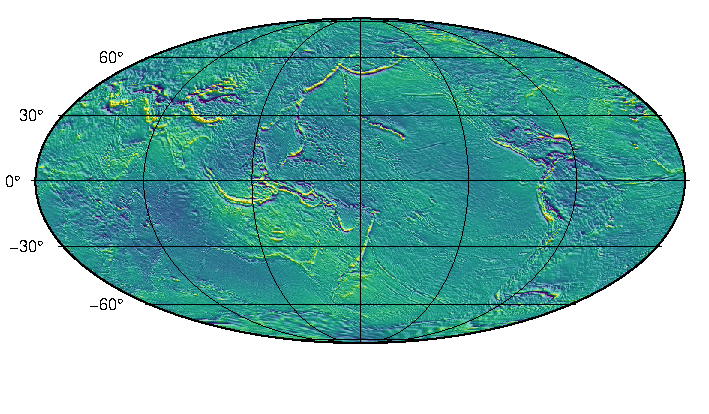
\includegraphics{./fig-gravity-disturbance-on-grs80-x.pdf}
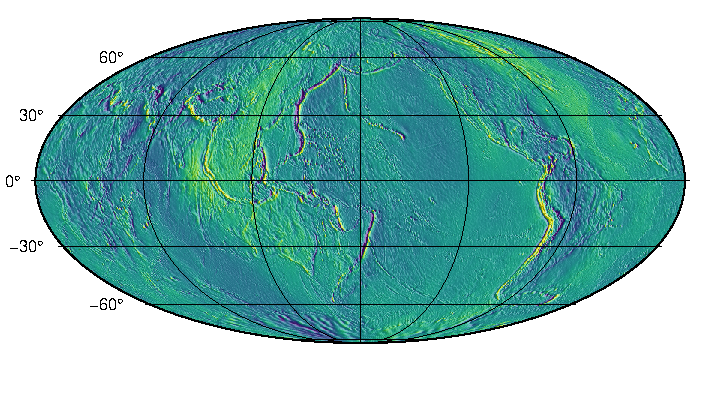
\includegraphics{./fig-gravity-disturbance-on-grs80-y.pdf}
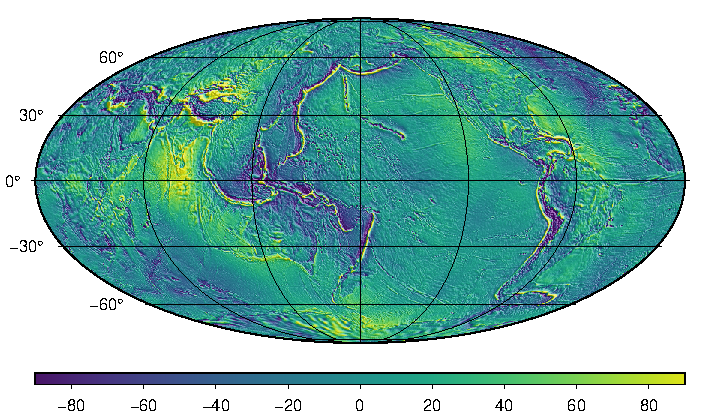
\includegraphics{./fig-gravity-disturbance-on-grs80-z.pdf}
\caption{Prvky vektora poruchy tiažového zrýchlenia $\delta g_{x^\mathrm{s}}$ 
(vrchná mapa), $\delta g_{y^\mathrm{s}}$ (prostredná mapa) a~$\delta 
g_{z^\mathrm{s}}$ (spodná mapa)~(jednotky~$\mathrm{mGal}$) zemského 
gravitačného poľa vypočítaného zo sférického harmonického modelu EIGEN-6C4 do 
stupňa~720 na povrchu elipsoidu~GRS80.  Normálny gravitačný potenciál je 
generovaný ekvipotenciálnym elipsoidom~GRS80.}
\label{fig:dg_ggm_grs80}
\end{figure}

Obrázok~\ref{fig:dg_ggm_450km} znázorňuje prvky vektora poruchy tiažového 
zrýchlenia vo výške~$450$~km nad elipsoidom GRS80.  Z~obrázku je zrejmé, že 
porucha tiažového zrýchlenia sa citeľne vyhlaďuje s~narastajúcou vzdialenosťou 
od Zeme.  Toto vyhladzovanie je dokonca rýchlejšie ako v~prípade poruchového 
potenciálu (porovnaj s~Obrázkami~\ref{fig:disturbing_potential_on_grs80} 
a~\ref{fig:disturbing_potential_at_450km}), pretože gravitačné zrýchlenie klesá 
s~druhou mocninou vzdialenosti (pozri rovnicu~\ref{eq:gg_body}), zatiaľ čo 
gravitačný potenciál klesá s~prvou mocninou vzdialenosti výpočtového bodu od 
diferenciálneho hmotného elementu (rovnica~\ref{eq:vg_body}).

\begin{figure}
\centering
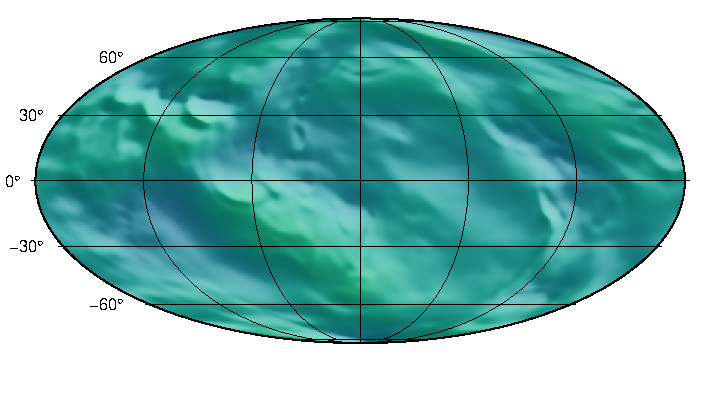
\includegraphics{./fig-gravity-disturbance-at-450km-x.pdf}
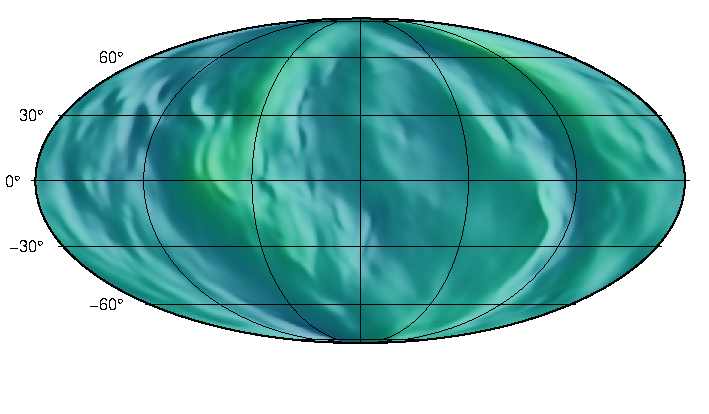
\includegraphics{./fig-gravity-disturbance-at-450km-y.pdf}
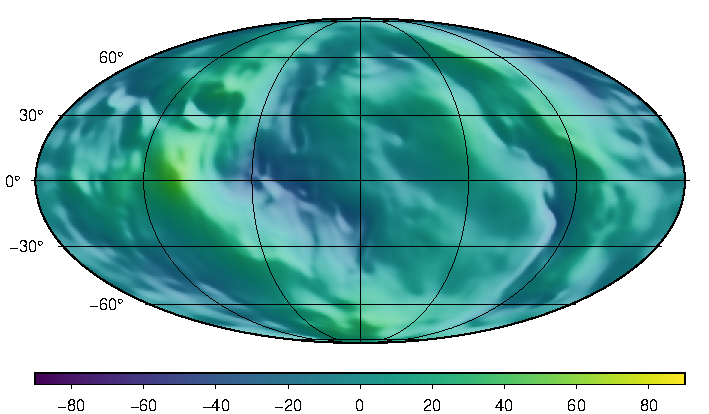
\includegraphics{./fig-gravity-disturbance-at-450km-z.pdf}
\caption{Prvky vektora poruchy tiažového zrýchlenia $\delta g_{x^\mathrm{s}}$ 
(vrchná mapa), $\delta g_{y^\mathrm{s}}$ (prostredná mapa) a~$\delta 
g_{z^\mathrm{s}}$ (spodná mapa)~(jednotky~$\mathrm{mGal}$) získané rovnakým 
spôsobom ako na~Obrázku~\ref{fig:dg_ggm_grs80} avšak vo výške~$450\ 
\mathrm{km}$ nad elipsoidom~GRS80.  Na oboch obrázkoch je použitá rovnaká 
farebná škála.}
\label{fig:dg_ggm_450km}
\end{figure}

Porucha tiažového zrýchlenia sa spravidla udáva v~jednotke mGal a~nadobúda 
hodnoty v~rozsahu od~$-400\ \mathrm{mGal}$ do $1000\ \mathrm{mGal}$ (hrubý 
odhad na základe modelu~EIGEN-6C4).  Vo fyzikálnej geodézii vystupuje zväčša 
ako meraná veličina, z~ktorej sa snažíme určiť poruchový potenciál a~následne 
priebeh geoidu.  Jedným z~cieľov je preto vyjadriť poruchový potenciál~$T$ 
z~rovníc~(\ref{eq:dg_vector}) či~(\ref{eq:dg_normals}).





\section{Anomália tiažového zrýchlenia}
\label{sec:gravity_anomaly}

S~tiažovým zrýchlením~$\vec g(P)$ sú spojené až dve veličiny poruchového poľa: 
porucha tiažového zrýchlenia~$\delta \vec g(P)$ 
(Kapitola~\ref{sec:gravity_disturbance}) a~\emph{anomália tiažového 
zrýchlenia}~$\Delta \vec g(P)$.  Vektor anomálie tiažového zrýchlenia je 
definovaný ako rozdiel vektora skutočného tiažového zrýchlenia~$\vec g(P)$ 
v~bode~$P$ a~vektora normálneho tiažového zrýchlenia~$\boldsymbol\gamma(Q)$ 
\emph{v~bode~$Q$} (Obrázok~\ref{fig:gravity_anomaly}),
%
\begin{equation}
\label{eq:Dg_vector_earth}
\Delta \vec g(P) = \vec g(P) - \boldsymbol\gamma (Q).
\end{equation}

\begin{figure}[bt]
\centering
\input{./fig-gravity-anomaly.pdf_tex}
\caption{Vektory definujúce anomálie tiažového zrýchlenia na povrchu 
Zeme,~$\Delta \vec g(P) = \vec g(P) - \boldsymbol \gamma(Q)$, a~na geoide, 
$\Delta \vec g(P_0) = \vec g(P_0) - \boldsymbol\gamma(Q_0)$.  Skutočná 
tiažnica~$t_W$ a~normálna tiažnica~$t_U$ sú z~vizualizačných dôvodov výrazne 
zakrivené voči normále k~elipsoidu~$n_e$.  V~skutočnosti majú~všetky tri línie 
blízky priebeh.}
\label{fig:gravity_anomaly}
\end{figure}

Bod~$Q$ získame nasledovne.  Nech bodom~$P$ prechádza normálna tiažnica~$t_U$.  
Bod~$Q$ je taký bod na tiažnici~$t_U$, pre ktorý platí~$U(Q) = W(P)$.  
Vzdialenosť medzi bodmi $Q$ a~$P$, meraná v~aproximácii po normále~$n_e$, sa 
nazýva \emph{výšková anomália} a~budeme ju označovať symbolom~$\zeta$ 
(Obrázok~\ref{fig:heights}).  Keď zostrojíme výškovú anomáliu pre každý bod na 
zemskom povrchu, získame plochu, ktorú budeme nazývať \emph{teluroid}.  
Teluroid predstavuje aproximáciu zemského povrchu.  Výšková anomália~$\zeta$ 
nadobúda celosvetovo hodnoty približne od~$-100$~m do~$100$~m, podobne ako 
výška geoidu nad referenčným elipsoidom (pozri 
Kapitolu~\ref{sec:disturbing_field_deflections}).  \emph{Teluroid ale na 
rozdiel od geoidu nie je ekvipotenciálnou plochou}.

Dôvod zavedenia anomálie tiažového zrýchlenia je najmä historický.  Ak chceme 
určiť poruchu tiažového zrýchlenia v~bode~$P$, potrebné je odmerať tiažové 
zrýchlenie v~bode~$P$ a~polohu bodu~$P$ voči ekvipotenciálnemu elipsoidu.  
Znalosť polohy je potrebná kvôli výpočtu normálneho tiažového zrýchlenia 
(Kapitola~\ref{sec:normal_gravity_field}).  Zo súradníc definujúcich~polohu 
potrebujeme poznať spravidla elipsoidickú šírku~$\phi$ a~elipsoidickú výšku~$h$ 
(Kapitola~\ref{sec:normal_gravity_taylor}).  V~súčasnosti už môže byť 
elipsoidická výška odmeraná jednoducho pomocou GNSS.  V~preddružicovej ére však 
bolo možné odmerať iba fyzikálne výšky pomocou nivelácie (pozri 
Kapitolu~\ref{sec:potential_differences}), v~tomto prípade dĺžku normálnej 
tiažnice~$t_U$ medzi bodmi~$Q_0$ a~$Q$ (Obrázok~\ref{fig:gravity_anomaly}).  
Táto vzdialenosť sa nazýva \emph{normálna výška podľa Molodenského}~$H_n$ 
\parencite{MoritzPhysicalGeodesy}.\footnote{Niveláciou je možné určiť aj iné 
typy fyzikálnych výšok \parencite[pozri napríklad][]{MoritzPhysicalGeodesy}.}  
Normálne tiažové zrýchlenie tak bolo možné vypočítať v~bode~$Q$ z~výšky~$H_n$ 
určenej niveláciou.  S~ohľadom na súčasnú dostupnosť globálnych navigačných 
družicových systémov je možné očakávať, že v~budúcnosti bude vo fyzikálnej 
geodézii dominovať porucha tiažového zrýchlenia 
\parencite{MoritzPhysicalGeodesy}.  V~súčasnosti sa bežne stretávame s~poruchou 
tiažového zrýchlenia aj s~anomáliou tiažového zrýchlenia.

\begin{figure}[bt]
\centering
\input{./fig-heights.pdf_tex}
\caption{Ortometrická výška~$H_o$ a~normálna výška podľa Molodenského~$H_n$ 
merané v~elipsoidickej aproximácii po normále k~elipsoidu prechádzajúcej 
bodom~$P$.  Ortometrická výška~$H_o$ je v~skutočnosti dĺžka skutočnej 
tiažnice~$t_W$ medzi bodmi~$P_0$ a~$P$ a~normálna výška podľa Molodenského je 
dĺžka normálnej tiažnice~$t_U$ medzi bodmi~$Q_0$ a~$Q$ (pozri 
Obrázok~\ref{fig:gravity_anomaly}).}
\label{fig:heights}
\end{figure}

Hoci vektory~$\vec g$ a~$\boldsymbol\gamma$ sú 
v~rovnici~(\ref{eq:Dg_vector_earth}) počítané v~dvoch rôznych bodoch, vektor 
anomálie tiažového zrýchlenia~$\Delta \vec g$ budeme formálne pripisovať 
bodu~$P$, čomu zodpovedá zápis~$\Delta \vec g(P)$, ktorý používame.

Vektor anomálie tiažového zrýchlenia môže byť definovaný aj na geoide vzťahom 
(Obrázok~\ref{fig:gravity_anomaly})
%
\begin{equation}
\label{eq:Dg_vector_geoid}
\Delta \vec g(P_0) = \vec g(P_0) - \boldsymbol\gamma(Q_0){.}
\end{equation}
%
Aj v~tomto prípade platí rovnosť medzi normálnym a~skutočným tiažovým 
potenciálom na ekvipotenciálnom elipsoide v~bode~$Q_0$ a~na geoide 
v~bode~$P_0$, $U(Q_0) = W(P_0)$ (pozri 
Kapitolu~\ref{sec:normal_gravity_field}), podobne ako platí rovnosť $U(Q) 
= W(P)$ v~súvislosti s~anomáliou tiažového zrýchlenia na povrchu 
Zeme~(\ref{eq:Dg_vector_earth}).  Anomálie~$\Delta \vec g(P)$ sa vo fyzikálnej 
geodézii využívajú prevažne na určenie výškovej anomálie~$\zeta$, ktorá je 
spätá s~normálnou výškou podľa Molodenského~$H_n$.  Anomálie~$\Delta \vec 
g(P_0)$ sa využívajú najmä na určovanie geoidu, ktorý je referenčnou plochou 
pre \emph{ortometrickú výšku}~$H_o$.  Ortometrická výška je dĺžka skutočnej 
tiažnice~$t_W$ medzi bodmi~$P_0$ a~$P$ (pozri Obrázok~\ref{fig:gravity_anomaly} 
a~tiež Kapitolu~\ref{sec:physical_heights}).

Okrem vektorovej anomálie tiažového zrýchlenia sa často stretávame aj so 
skalárnou definíciou anomálie tiažového zrýchlenia (pozri tiež 
Kapitolu~\ref{sec:gravity_disturbance}), či už na povrchu Zeme
%
\begin{equation}
\label{eq:Dg_scalar_earth}
\Delta g(P) = \| \vec g(P) \| - \| \boldsymbol \gamma (Q) \| = g(P) 
- \gamma(Q){.}
\end{equation}
%
alebo na geoide,
%
\begin{equation}
\label{eq:Dg_scalar_geoid}
\Delta g(P_0) = \| \vec g(P_0) \| - \| \boldsymbol \gamma (Q_0) \| = g(P_0) 
- \gamma(Q_0){.}
\end{equation}
%
Podobne ako v~súvislosti s~poruchou tiažového zrýchlenia 
(Kapitola~\ref{sec:gravity_disturbance}), aj tentokrát platí
%
\begin{equation}
\| \Delta \vec g(P) \| \neq \Delta g(P){,}
\end{equation}
%
\begin{equation}
\| \Delta \vec g(P_0) \| \neq \Delta g(P_0){.}
\end{equation}

Anomália tiažového zrýchlenia sa väčšinou udáva v~jednotke~mGal.  Anomália 
a~porucha tiažového zrýchlenia sú základné merateľné veličiny fyzikálnej 
geodézie, z~ktorých sa určuje tvar Zeme.

\subsection{Vzťah medzi anomáliou tiažového zrýchlenia a~poruchovým 
potenciálom}

Nájdime teraz vzťah medzi anomáliou tiažového zrýchlenia a~poruchovým 
potenciálom, podobne ako sme našli vzťah medzi poruchou tiažového zrýchlenia 
a poruchovým potenciálom (rovnica~\ref{eq:dg_normals}).  Tentokrát situáciu 
komplikuje rozdielna poloha bodov~$P$ a~$Q$ 
v~rovnici~(\ref{eq:Dg_scalar_earth}) a~zakrivenie normálnej tiažnice.  Úlohu si 
výrazne zjednodušíme linearizáciou problému a~využitím elipsoidickej 
aproximácie z~Obrázku~\ref{fig:heights}.  Obe aproximácie sú postačujúce pre 
praktické aplikácie \parencite{MoritzAdvancedGeodesy}.  Následne odvodíme vzťah 
medzi oboma veličinami aj vo sférickej aproximácii.  Exaktné riešenie bolo 
nájdené v~prácach~\textcite{Meissl1971b} a~\textcite{Borre_chapter8} 
\parencite[pozri tiež napríklad][]{MoritzAdvancedGeodesy,Janak2006}.

\subsubsection{Elipsoidická aproximácia}

Hľadať budeme najprv vzťah medzi~$\Delta g(P_0)$ a~$T(P_0)$ v~bode~$P_0$ na 
geoide.  Rozviňme~$\gamma$ do Taylorovho radu v~bode~$Q_0$ a~následne 
zanedbajme členy druhého a~vyšších rádov, ktorých vplyv je malý,
%
\begin{equation}
\label{eq:gamma_P0}
\gamma(P_0) = \sum_{i = 0}^\infty \frac{1}{i!} \, \left.\frac{\partial^i 
\gamma}{\partial h^i}\right|_{Q_0} \, N^i \approx \gamma(Q_0) 
+ \left.\frac{\partial \gamma}{\partial h}\right|_{Q_0} \, N{.}
\end{equation}
%
Dosadením~(\ref{eq:gamma_P0}) do~(\ref{eq:Dg_scalar_geoid}) dostaneme 
v~kombinácii s~(\ref{eq:dg_normals}) vzťah
%
\begin{equation}
\label{eq:Dg_T_tmp}
\begin{split}
\Delta g(P_0) &= g(P_0) - \gamma(P_0) + \left.\frac{\partial \gamma}{\partial 
h}\right|_{Q_0} \, N = \delta g(P_0) + \left.\frac{\partial \gamma}{\partial 
h}\right|_{Q_0} \, N\\
%
&=-\left.\frac{\partial T}{\partial h}\right|_{P_0} + \left.\frac{\partial 
\gamma}{\partial h}\right|_{Q_0} \, N{.}
\end{split}
\end{equation}
%
Rovnica~(\ref{eq:Dg_T_tmp}) popisuje, okrem iného, vzťah medzi poruchou 
a anomáliou tiažového zrýchlenia.  Výšku geoidu nad referenčným elipsoidom~$N$ 
ďalej získame rozvojom normálneho tiažového potenciálu do Taylorovho radu 
v~bode~$Q_0$,
%
\begin{equation}
\label{eq:U_P0}
U(P_0) = \sum_{i = 0}^\infty \frac{1}{i!} \, \left.\frac{\partial^i U}{\partial 
h^i}\right|_{Q_0} \, N^i \approx U(Q_0) + \left.\frac{\partial U}{\partial 
h}\right|_{Q_0} \, N = U(Q_0) - \gamma(Q_0) \, N{.}
\end{equation}
%
S uvážením $W(P_0) = U(Q_0)$ (pozri Kapitolu~\ref{sec:normal_gravity_field}) 
a~vzťahu~(\ref{eq:disturbing_potential}) môžeme prepísať 
rovnicu~(\ref{eq:U_P0}) do tvaru
%
\begin{equation}
\label{eq:N}
N = \frac{T(P_0)}{\gamma(Q_0)}.
\end{equation}
%
Vzťah~(\ref{eq:N}) sa nazýva \emph{Brunsov vzorec} a~umožňuje vypočítať 
geometrický parameter, výšku geoidu nad referenčným elipsoidom~$N$, 
z~fyzikálneho parametra, ktorým je poruchový potenciál~$T(P_0)$ na geoide.  
Brunsov vzorec je základom určovania geoidu.  Dodajme, že zanedbanie členov 
druhého a~vyšších rádov v~rovnici~(\ref{eq:U_P0}) spôsobuje chyby v~určení~$N$ 
na úrovni niekoľko málo milimetrov \parencite{Jekeli2015,Sjoberg2017}, teda 
zhruba o~rád menšie ako je súčasná (približne centimetrová) presnosť určenia 
geoidu.  Je potrebné tiež zdôrazniť, že vzťah~(\ref{eq:N}) bol získaný za 
predpokladu~$U_0 = W_0$.  Ak $U_0 \neq W_0$, túto nerovnosť je potrebné 
zohľadniť v~procese odvodenia vzťahu pre~$N$ \parencite[pozri 
napríklad][]{VanicekGeodesy}.

Dosadením~(\ref{eq:N}) do~(\ref{eq:Dg_T_tmp}) získame hľadaný vzťah medzi 
anomáliou tiažového zrýchlenia a~poruchovým potenciálom,
%
\begin{equation}
\label{eq:Dg_fundamental_equation_geoid}
\Delta g(P_0) = -\left.\frac{\partial T}{\partial h}\right|_{P_0} 
+ \frac{1}{\gamma(Q_0)} \, \left.\frac{\partial \gamma}{\partial 
h}\right|_{Q_0} \, T(P_0){.}
\end{equation}
%
Rovnica~(\ref{eq:Dg_fundamental_equation_geoid}) sa nazýva \emph{základná 
rovnica fyzikálnej geodézie}.

Podobným spôsobom možno napísať základnú rovnicu fyzikálnej geodézie pre 
anomáliu tiažového zrýchlenia na povrchu Zeme,
%
\begin{equation}
\label{eq:Dg_fundamental_equation_earth}
\Delta g(P) = -\left.\frac{\partial T}{\partial h}\right|_{P} 
+ \frac{1}{\gamma(Q)} \, \left.\frac{\partial \gamma}{\partial h}\right|_{Q} \, 
T(P){.}
\end{equation}
%
Na získanie vzťahu~(\ref{eq:Dg_fundamental_equation_earth}) sme využili 
\emph{zovšeobecnený Brunsov vzorec}
%
\begin{equation}
\label{eq:zeta}
\zeta = \frac{T(P)}{\gamma(Q)}{,}
\end{equation}
%
ktorý je možné získať podobne ako vzťah~(\ref{eq:N}).

Anomáliu tiažového zrýchlenia možno definovať v~širšom zmysle nielen pre body 
na povrchu Zeme alebo na geoide, ale aj pre body mimo Zeme.  Symbol~$P$ potom 
označuje bod, v~ktorom je dané tiažové zrýchlenie~$g(P)$ 
v~rovnici~(\ref{eq:Dg_scalar_earth}) a~bod~$Q$ je daný priesečníkom normálnej 
tiažnice prechádzajúcej bodom~$P$ a~normálnej ekvipotenciálnej plochy 
s~normálnym tiažovým potenciálom~$U(Q) = W(P)$ 
\parencite{MoritzPhysicalGeodesy}.  Odvodením získame aj v~tomto prípade 
vzťah~(\ref{eq:Dg_fundamental_equation_earth}), ktorý využíva elipsoidickú 
aproximáciu.  Potom body $P$ a~$Q$ ležia na normále k~ekvipotenciálnemu 
elipsoidu, ktorá prechádza bodom~$P$, pričom pre polohu bodu~$Q$ platí $U(Q) 
= W(P)$.  Pre kvantifikáciu efektu linearizácie na anomáliu tiažového 
zrýchelnia pozri napríklad prácu \textcite{Claessens2006}.

\subsubsection{Sférická aproximácia}

Aproximujme deriváciu v~smere elipsoidickej normály~$\partial \slash \partial 
h$ v~rovnici~(\ref{eq:Dg_fundamental_equation_earth}) deriváciou v~smere 
sprievodiča~$\partial \slash \partial r$,
%
\begin{equation}
\Delta g(P) = -\left.\frac{\partial T}{\partial r}\right|_{P} 
+ \frac{1}{\gamma(Q)} \, \left.\frac{\partial \gamma}{\partial r}\right|_{Q} \, 
T(P){.}
\end{equation}
%
Keďže člen
%
\begin{equation}
\label{eq:Dg_fundamental_equation_earth_term}
\left.\frac{1}{\gamma(Q)} \, \frac{\partial \gamma}{\partial r}\right|_Q
\end{equation}
%
nadobúda malé hodnoty, môžeme pre jednoduchosť uvažovať normálne tiažové 
zrýchlenie~$\gamma$ generované nerotujúcou homogénnou guľou.  Zo~vzťahu pre 
potenciál nerotujúcej homogénnej gule~(\ref{eq:vg_sh_0degree}) potom vyplýva
%
\begin{align}
U &= \frac{GM}{r}{,}\\
%
\gamma &= -\frac{\partial U}{\partial r} = \frac{GM}{r^2}{,}\\
%
\frac{\partial \gamma}{\partial r} &= -2 \, \frac{GM}{r^3}{,}
\end{align}
%
a tak môžeme prepísať~(\ref{eq:Dg_fundamental_equation_earth_term}) do tvaru
%
\begin{equation}
\left.\frac{1}{\gamma(Q)} \, \frac{\partial \gamma}{\partial r}\right|_Q 
\approx \left.\frac{r^2}{GM} \, \left( -2\frac{GM}{r^3} \right)\right|_Q 
= -\left.\frac{2}{r}\right|_Q {.}
\end{equation}
%
Sférická aproximácia anomálie tiažového zrýchlenia je potom daná vzťahom
%
\begin{equation}
\label{eq:Dg_fundamental_equation_earth_sph}
\Delta g(P) = -\left.\frac{\partial T}{\partial r}\right|_{P} 
- \left.\frac{2}{r}\right|_{P} \, T(P){,}
\end{equation}
%
pričom sme pre zjednodušenie využili približnú rovnosť
%
\begin{equation}
\left.\frac{2}{r}\right|_Q \, T(P) \approx \left.\frac{2}{r}\right|_P \, 
T(P){.}
\end{equation}

Sférická aproximácia anomálie a~poruchy tiažového zrýchlenia spôsobuje chybu 
v~určení výšky geoidu nad referenčným elipsoidom~$N$ zhruba na úrovni $0.003 \, 
N$ \parencite{MoritzPhysicalGeodesy}.  Pri dosahovaných hodnotách $N$ zhruba od 
$-100$ do $100$~m tak ide o~chybu menšiu ako 1~m v~určení geoidu.  Pre presný 
výpočet geoidu tak už v~súčasnosti nie je sférická aproximácia anomálie 
a~poruchy tiažového zrýchlenia postačujúca.


\subsection{Sférický harmonický rozvoj anomálie tiažového zrýchlenia}

Presný rozvoj anomálie tiažového zrýchlenia do radu sférických harmonických 
funkcií je kvôli zložitosti~jej definície náročný \parencite[pozri 
napríklad][]{Barthelmes2013}.  Uvedieme preto iba rozvoj vo sférickej 
aproximácii.  Dosadením~(\ref{eq:t_sh}) 
do~(\ref{eq:Dg_fundamental_equation_earth_sph}) získame
%
\begin{equation}
\label{eq:Dg_sh_sa}
\Delta g(P) = \frac{GM}{R^2} \sum_{n = 0}^\infty (n - 1) \, \left( \frac{R}{r} 
\right)^{n + 2} \sum_{k = -n}^{n} \bar{t}_{nk} \, \bar{Y}_{nk}(\varphi, 
\lambda){.}
\end{equation}
%
Vo sférickej aproximácii sa tak anomália tiažového 
zrýchlenia~(\ref{eq:Dg_sh_sa}) odlišuje od poruchy tiažového 
zrýchlenia~(\ref{eq:dg_sh_sa} a~\ref{eq:dgz_sh}) iba v~člene~$(n - 1)$, ktorý 
nahradil člen~$(n + 1)$.  Všimnime si, že  koeficienty~$\bar{t}_{nk}$ stupňa~$n 
= 1$ neovplyvňujú anomáliu tiažového zrýchlenia v~dôsledku nulového člena~$(n 
- 1)$.

Anomália tiažového zrýchlenia a~porucha tiažového zrýchlenia nadobúdajú podobné 
hodnoty, preto sme vyobrazenie anomálie tiažového zrýchelenia vynechali (pozri 
priebeh poruchy tiažového zrýchlenia na Obrázkoch~\ref{fig:dg_ggm_grs80} 
a~\ref{fig:dg_ggm_450km}).



\subsection*{Dve poznámky k~anomálii tiažového zrýchlenia}

V~súvislosti s~odvodením Brunsovho vzorca a~základnej rovnice fyzikálnej 
geodézie sa zdá byť vhodné opäť zdôrazniť dôležitosť voľby normálneho poľa.  Ak 
by bolo normálne pole zvolené nevhodne, teda rozdiely medzi skutočným 
a~normálnym poľom by s~ohľadom na súčasnú presnosť nemohli byť považované za 
lineárne, nebolo by možné obmedziť rozvoje~(\ref{eq:gamma_P0}) 
a~(\ref{eq:U_P0}) iba na prvé dva členy.  Pridanie už i~len kvadratického člena 
výrazne komplikuje úlohu.

Druhá poznámka sa týka anomálií tiažového zrýchlenia na geoide~$\Delta g(P_0)$, 
ku ktorým sme uviedli, že slúžia najmä na výpočet geoidu.  Tieto anomálie sú, 
samozrejme, merané na povrchu Zeme vo forme~$\Delta g(P)$ a~až následne sú 
matematicky zredukované na geoid.  Z~Kapitoly~\ref{sec:harmonic_function} 
vieme, že táto úloha, nazývaná analytické pokračovanie nadol, je numericky 
nestabilná.  To znamená, že v~princípe ju nie je možné vyriešiť bez nejakej 
formy stabilizácie.  Tou môže byť napríklad mierne vyhladenie dát či zníženie 
rozlíšenia daného problému.  Stabilizácia ale spôsobí, že v~skutočnosti získame 
riešenie inej úlohy ako tej, ktorá bola formulovaná 
\parencite{SansoGeodeticBoundaryValueProblem}, hoci získané riešenie môže byť 
rozumne blízke hľadanému riešeniu.  Aby bolo možné potlačiť odchýlky od 
hľadaného riešenia, je potrebné zvyšovať presnosť a~rozlíšenie vstupných 
údajov, čo je v~praktických aplikáciách problematické kvôli náročnosti 
získavania meraných dát.  Redukcia anomálií tiažového zrýchlenia zo zemského 
povrchu na geoid tak patrí medzi najnáročnejšie časti určovania geoidu.






\section{Zvislicové odchýlky}
\label{sec:deflections}

V~Kapitolách~\ref{sec:gravity_disturbance} a~\ref{sec:gravity_anomaly} sme 
videli, že jedna z~merateľných veličín fyzikálnej geodézie, tiažové zrýchlenie, 
súvisí s~poruchovým potenciálom, a~teda aj s~určovaným tvarom Zeme (pozri 
rovnicu~\ref{eq:N}).  Medzi časté geodetické merania ale patrí aj určovanie 
polohy bodu na povrchu Zeme pomocou astronomických meraní a~pomocou globálnych 
navigačných družicových systémov.  Bolo by preto výhodné, ak by sme našli aj 
vzťah medzi týmito meraniami a~poruchovým potenciálom, pretože by to umožnilo 
určovať tvar Zeme z~ďalšieho typu geodetických meraní.  Hoci to na prvý pohľad 
nemusí byť zrejmé, takýto vzťah naozaj existuje.  Na jeho nájdenie zavedieme 
veličinu, ktorú budeme nazývať \emph{zvislicová odchýlka}.

Zvislicová odchýlka je uhol medzi skutočnou zvislicou (pozri 
Kapitolu~\ref{sec:plumbline}) a~zvoleným referenčným smerom 
\parencite{TorgeGeodesy}.  Referenčný smer často závisí od aplikácie, preto sa 
v~literatúre môžeme stretnúť s~rozličnými definíciami zvislicových odchýlok 
(Obrázok~\ref{fig:deflections}).

\begin{figure}[bt]
\centering
\input{./fig-deflections.pdf_tex}
\caption{Helmertova zvislicová odchýlka~$\Theta^\textrm{Helmert}$, Molodenského 
zvislicová odchýlka~$\Theta^\textrm{Molodenskij}$ a~Pizzettiho zvislicová 
odchýlka~$\Theta^\textrm{Pizzetti}$.  Symbol~$t_W^P$ označuje skutočnú tiažnicu 
prechádzajúcu bodom~$P$ na povrchu Zeme.  Tiažnica~$t_W^P$ je identická so 
skutočnou tiažnicou~$t_W^{P_0}$, ktorá prechádza bodom~$P_0$ na geoide.  
Symboly~$z_W^P$ a~$z_W^{P_0}$ označujú skutočné zvislice v~bodoch~$P$ a~$P_0$.  
Zvislicou rozumieme dotyčnicu k~tiažnici, v~tomto prípade v~bodoch~$P$ a~$P_0$ 
(pozri Kapitolu~\ref{sec:plumbline}).  Symbol~$n$ označuje normálu, pričom 
dolný index označuje plochu, na ktorú je normála kolmá ($e$ pre elipsoid, $U$ 
pre normálnu ekvipotenciálnu plochu~$U = \textrm{kon\v{s}t.}$), a~horný index 
označuje bod, cez ktorý normála prechádza.  Poznamenajme, že normála~$n_U^P$ 
nie je totožná s~\emph{normálnou} zvislicou~$z_U^Q$, hoci sú si veľmi blízke.}
\label{fig:deflections}
\end{figure}

\begin{itemize}
\item \emph{Helmertova zvislicová odchýlka}~$\Theta^\mathrm{Helmert}$ je uhol 
medzi skutočnou zvislicou~$z_W^P$ prechádzajúcou~bodom~$P$ na povrchu Zeme 
a~normálou k~elipsoidu~$n_e^P$ prechádzajúcou bodom~$P$.  Táto zvislicová 
odchýlka sa tiež zvykne nazývať \textit{astronomicko--geodetická zvislicová 
odchýlka} \parencite{Jekeli1999b}.

\item \emph{Molodenského zvislicová odchýlka}~$\Theta^\mathrm{Molodenskij}$ je 
uhol medzi skutočnou zvislicou~$z_W^P$ prechádzajúcou bodom~$P$ na povrchu Zeme 
alebo mimo nej a~normálou~$n_U^P$ k~takej normálnej ekvipotenciálnej 
ploche~$U(Q) = \textrm{kon\v{s}t.}$, ktorej normálny tiažový potenciál~$U(Q)$ 
je rovný skutočnému tiažovému potenciálu~$W(P)$, pričom normála~$n_U^P$ 
prechádza bodom~$P$.

\item \emph{Pizzettiho zvislicová odchýlka}~$\Theta^\mathrm{Pizzetti}$ je uhol 
medzi skutočnou zvislicou~$z_W^{P_0}$ prechádzajúcou bodom~$P_0$ na povrchu 
geoidu a~normálou k~elipsoidu~$n_e^{P_0}$ prechádzajúcou bodom~$P_0$.

\item \emph{Gravimetrická zvislicová odchýlka}~$\Theta^\mathrm{grav}$ je uhol 
medzi vektorom skutočného tiažového zrýchlenia~$\vec g(P)$ v~bode~$P$ 
a~vektorom normálneho tiažového zrýchlenia~$\boldsymbol\gamma(P)$ v~bode~$P$ 
(Obrázok~\ref{fig:gravity_disturbance}).\footnote{Uhol medzi vektormi~$\vec 
g(P)$ a~$\boldsymbol\gamma(Q)$ (pozri Obrázok~\ref{fig:gravity_anomaly}) je 
vzhľadom na malé zakrivenie normálnej tiažnice a~vzhľadom na krátku vzdialenosť 
medzi bodmi~$P$ a~$Q$ veľmi podobný uhlu medzi vektormi~$\vec g(P)$ 
a~$\boldsymbol\gamma(P)$ (Obrázok~\ref{fig:gravity_disturbance}).  V~mnohých 
situáciách preto nie je potrebné rozlišovať, či je gravimetrická zvislicová 
odchýlka daná vektormi~$\vec g(P)$ a~$\boldsymbol\gamma(P)$ alebo~$\vec g(P)$ 
a~$\boldsymbol\gamma(Q)$.}
\end{itemize}
%
Rozdiel medzi Helmertovou a~Molodenského zvislicovou odchýlkou je spôsobený 
zakrivením normálnej tiažnice \parencite{Jekeli1999b}.  Zvislicové 
odchýlky~$\Theta$ nadobúdajú hodnoty od $0'$ v~rovinatom teréne do 
približne~$2'$ v~najväčších pohoriach na Zemi \parencite{GGMplus}, zvyčajne 
však najviac približne niekoľko desiatkok uhlových sekúnd.

Nech je daný súradnicový systém, v~ktorom je smer skutočnej zvislice určený 
astronomickými súradnicami~$\Phi$ a~$\Lambda$.  Nech je ďalej daný referenčný 
elipsoid, voči ktorému sú určované súradnice~$\varphi$ a~$\lambda$ referenčného 
smeru zvislicovej odchýlky.  Predpokladajme, že osi~$Z$ oboch súradnicových 
systémov sú rovnobežné a~rovnako tak sú rovnobežné aj roviny ich nultých 
poludníkov \parencite{TorgeGeodesy}.\footnote{Súčasné súradnicové systémy 
zabezpečujú splnenie týchto podmienok s~dostatočnou presnosťou.  Riešenie pre 
súradnicové systémy, ktoré tieto podmienky nespĺňajú, je možné nájsť napríklad 
v~práci \textcite{Pick2000}.}  Rovnobežným posunutím takéhoto súradnicového 
systému do bodu~$P$, v~ktorom určujeme zvislicovú odchýlku, získame situáciu 
znázornenú na Obrázku~\ref{fig:deflections_unit_sphere}.

Zvislicovú odchýlku je možné matematicky popísať rozličnými spôsobmi, z~ktorých 
dva sú obzvlášť výhodné (Obrázok~\ref{fig:deflections_unit_sphere}).  Jeden 
využíva veľkosť uhlového vychýlenia~$\Theta$ medzi skutočnou zvislicou 
a~referenčným smerom a~azimut~$\alpha$, ktorý udáva smer vychýlenia v~rovine 
lokálneho horizontu.  Druhý prístup rozkladá zvislicovú odchýlku do dvoch 
kolmých smerov.  Jedna zložka zachytáva uhlový rozdiel medzi skutočnou 
zvislicou a~referenčným smerom po premietnutí zvislicovej odchýlky do~roviny 
meridiánu; budeme ju označovať symbolom~$\xi$.  Druhá zložka popisuje uhlový 
rozdiel medzi skutočnou zvislicou a~referenčným smerom po premietnutí do~roviny 
prvého vertikálu; označovať ju budeme symbolom~$\eta$.  Zvislicovú odchýlku 
preto môžeme chápať ako dvojrozmerný vektor~$\boldsymbol\Theta = [\xi, 
\eta]^\top$, ktorý má svoju veľkosť~$\Theta = \| \boldsymbol\Theta \|$ 
a~smer~$\alpha$.

\begin{figure}[bt]
\centering
\input{./fig-deflections-unit-sphere.pdf_tex}
\caption{Vektor zvislicovej odchýlky~$\boldsymbol\Theta$ na jednotkovej sfére 
so stredom v~bode~$P$, v~ktorom je určovaná zvislicová odchýlka.  Zvislicová 
odchýlka je znázornená v~podobe 1)~veľkosti~$\Theta = \| \boldsymbol\Theta \|$ 
a~azimutu~$\alpha$ a~2)~pravouhlých priemetov~$\xi$ a~$\eta$ do meridiánovej 
roviny a~do roviny prvého vertikálu.  Symboly~$\Phi$ a~$\Lambda$ označujú 
astronomické súradnice bodu~$P$, v~ktorom je určovaná zvislicová odchýlka 
(pozri Obrázok~\ref{fig:deflections}).  Symboly~$\phi$ a~$\lambda$ označujú 
elipsoidickú šírku a~elipsoidickú dĺžku bodu~$P$.  Referenčným smerom na~tomto 
obrázku je teda normála k~elipsoidu, ktorá prechádza bodom~$P$.}
\label{fig:deflections_unit_sphere}
\end{figure}

Zložky~$\xi$ a~$\eta$ získame z~Obrázku~\ref{fig:deflections_unit_sphere},
%
\begin{equation}
\begin{split}
\xi  &= \Phi - \phi{,}\\
\eta &= (\Lambda - \lambda) \, \cos\phi{.}
\end{split}
\end{equation}
%
Veľkosť zvislicovej odchýlky~$\Theta$ môžeme vypočítať sférickou kosínusovou 
vetou vo sférickom trojuholníku~$N$, $N_r$ a~$N'_r$ (pozri 
Obrázok~\ref{fig:deflections_unit_sphere}).  Keďže ale uhly~$\Theta$, $\xi$ 
a~$\eta$ nadobúdajú malé hodnoty (v~absolútnej hodnote nanajvýš približne 
$2'$), s~dostatočnou mierou aproximácie môžeme použiť kosínusovú vetu pre 
rovinný trojuholník,
%
\begin{equation}
\label{eq:deflection_total}
\Theta \approx \sqrt{\xi^2 + \eta^2 - 2\, \xi \, \eta \, \cos 90^{\circ}} 
= \sqrt{\xi^2 + \eta^2}{.}
\end{equation}
%
Použitím vzťahov sférickej trigonometrie 
\parencite[napríklad][]{MoritzPhysicalGeodesy},
%
\begin{equation}
\label{eq:deflection_aux}
\begin{split}
\sin\Theta \, \cos\alpha &= \cos\phi \, \sin\Phi - \sin\phi \, \cos\Phi \, 
\cos(\Lambda - \lambda){,}\\
\sin\Theta \, \sin\alpha &= \cos\Phi \, \sin(\Lambda - \lambda),
\end{split}
\end{equation}
%
získame azimut zvislicovej odchýlky 
(Obrázok~\ref{fig:deflections_unit_sphere}),
%
\begin{equation}
\tan\alpha = \frac{\cos\Phi \, \sin(\Lambda - \lambda)}{\cos\phi \, \sin\Phi 
- \sin\phi \, \cos\Phi \, \cos(\Lambda - \lambda)}{.}
\end{equation}
%
Pomocou známej hodnoty meridiánovej a~priečnej zložky zvislicovej odchýlky tiež 
môžeme zvislicovú odchýlku premietnuť do ľubovoľného smeru, ktorý je daný 
azimutom~$A$ (Obrázok~\ref{fig:deflections_projection}),
%
\begin{equation}
\label{eq:deflection_vareps}
\varepsilon = \xi \, \cos A + \eta \, \sin A{.}
\end{equation}

\begin{figure}[bt]
\centering
\input{./fig-deflections-projection.pdf_tex}
\caption{Priemet zvislicovej odchýlky~$\Theta = [\xi, \eta]^\top$ do spojnice 
s~azimutom~$A$ v~rovinnej aproximácii.}
\label{fig:deflections_projection}
\end{figure}

Okrem určovania tvaru Zeme majú zvislicové odchýlky praktické využitie aj 
v~ďalších geodetických úlohách.  Geodetické prístroje ako teodolit či nivelačný 
prístroj sa horizontujú preto, aby sa ich vertikálna os stotožnila so skutočnou 
zvislicou, ktorá prechádza stredom libely.  Merané vodorovné smery, vertikálne 
uhly či vertikálne prevýšenia sú tak vztiahnuté k~skutočnej zvislici, 
resp. skutočnému lokálnemu horizontu.  Keďže ale skutočné zvislice 
prechádzajúce dvoma rôznymi bodmi nie sú vo všeobecnosti rovnobežné, niektoré 
geodetické merania si môžu vyžadovať korekciu týchto efektov, obzvlášť ak je 
vyžadovaná presnosť vysoká.  Na výpočet takýto korekcii slúžia práve zvislicové 
odchýlky.  Ďalšie využitie zvislicových odchýlok je napríklad na navigáciu 
inerciálnych navigačných systémov \parencite[pozri napríklad][]{Jekeli2000}.


\subsection{Vzťah medzi zvislicovou odchýlkou a~poruchovým potenciálom}
\label{sec:deflections_disturbing_potential}

Na získanie vzťahu medzi zvislicovými odchýlkami a~poruchovým potenciálom 
budeme uvažovať gravimetrickú zvislicovú odchýlku pre jej priamočiaru súvislosť 
s~tiažovým poľom.  Pre jednoduchosť ju spolu s~jej zložkami budeme v~tejto 
kapitole označovať symbolmi~$\Theta$, $\xi$ a~$\eta$ bez horného indexu.

Gravimetrickú zvislicovú odchýlku sme definovali ako uhol medzi skutočnou 
a~normálnou zvislicou v~bode~$P$.  Keďže smer zvislice je totožný so smerom 
normály k~ekvipotenciálnej ploche, trojrozmerný vektor zvislicovej odchýlky je 
daný vzťahom \parencite{SansoGeoidDetermination},
%
\begin{equation}
\label{eq:deflection_eps}
\boldsymbol\varepsilon(P) = \vec n_W(P) - \vec n_U(P){,}
\end{equation}
%
kde $\vec n_W(P)$ a~$\vec n_U(P)$ sú jednotkové vektory \emph{vonkajších} 
normál ku~skutočnej a~normálnej ekvipotenciálnej ploche v~bode~$P$ (pozri 
Obrázok~\ref{fig:gravity_disturbance}).  Horizontálne zložky~$\varepsilon_x$, 
$\varepsilon_y$ vektora~$\boldsymbol\varepsilon = [\varepsilon_x, 
\varepsilon_y, \varepsilon_z]^\top$ predstavujú zložky~$\xi$ a~$\eta$ 
vektora~$\boldsymbol\Theta = [\xi, \eta]^\top$ (pozri 
Kapitolu~\ref{sec:deflections}), teda
%
\begin{equation}
\label{eq:xi_eta_eps}
\begin{split}
\xi = \varepsilon_x{,}\\
\eta = \varepsilon_y{.}
\end{split}
\end{equation}

Z~definície operátora gradient vyplýva, že jednotkové vektory~$\vec n_W(P)$ 
a~$\vec n_U(P)$ sú dané vzťahmi
%
\begin{equation}
\label{eq:nw_nu}
\begin{split}
\vec n_W(P) &= -\frac{\nabla W(P)}{\| \nabla W(P) \|} = -\frac{\nabla 
W(P)}{g(P)}{,}\\
%
\vec n_U(P) &= -\frac{\nabla U(P)}{\| \nabla U(P) \|} = -\frac{\nabla 
U(P)}{\gamma(P)}{.}
\end{split}
\end{equation}
%
Po dosadení do vzťahu~(\ref{eq:deflection_eps}) tak získame rovnicu
%
\begin{equation}
\label{eq:deflection_eps2}
\boldsymbol\varepsilon(P) = -\frac{\nabla W(P)}{g(P)} + \frac{\nabla 
U(P)}{\gamma(P)}{.}
\end{equation}
%
S~využitím vzťahov~(\ref{eq:gradient_additivity}), 
(\ref{eq:disturbing_potential}),  (\ref{eq:dg_scalar}) a~(\ref{eq:nw_nu}) 
môžeme ďalej upraviť túto rovnicu do tvaru
%
\begin{equation}
\label{eq:deflection_eps3}
\begin{split}
\boldsymbol\varepsilon(P) &= - \frac{\nabla W(P) - \nabla U(P)}{\gamma(P)} 
- \frac{\gamma(P) - g(P)}{\gamma(P)} \, \frac{\nabla W(P)}{g(P)}\\
%
&= - \frac{\nabla T(P)}{\gamma(P)} + \frac{\delta g(P)}{\gamma(P)} \, \vec 
n_W(P){.}\\
\end{split}
\end{equation}
%
Po uvážení~(\ref{eq:xi_eta_eps}) tak získame vzťahy
%
\begin{equation}
\label{eq:deflection_grav}
\begin{split}
\xi &= -\frac{1}{\gamma(P)} \, \left.\frac{\partial T}{\partial x}\right|_{P} 
+ \frac{1}{g(P)} \, \frac{\delta g(P)}{\gamma(P)} \, \left.\frac{\partial 
W}{\partial x}\right|_P = -\frac{T_x(P)}{\gamma(P)} + \frac{\delta 
g(P)}{\gamma(P)} \, \frac{W_x(P)}{g(P)}{,}\\
%
\eta &= -\frac{1}{\gamma(P)} \, \left.\frac{\partial T}{\partial y}\right|_{P} 
+ \frac{1}{g(P)} \, \frac{\delta g(P)}{\gamma(P)} \, \left.\frac{\partial 
W}{\partial y}\right|_P= -\frac{T_y(P)}{\gamma(P)} + \frac{\delta 
g(P)}{\gamma(P)} \, \frac{W_y(P)}{g(P)}{.}\\
\end{split}
\end{equation}
%
Rovnica~(\ref{eq:deflection_grav}) popisuje vzťah medzi lokálnymi 
charakteristikami tiažového poľa v~bode~$P$ na jednej strane a~zvislicovými 
odchýlkami v~bode~$P$ na strane druhej.

Zložky~$\varepsilon_x$ a~$\varepsilon_y$ z~rovnice~(\ref{eq:xi_eta_eps}) sme 
zámerne opísali vágnym prívlastkom \emph{horizontálne} bez toho, aby sme 
bližšie špecifikovali, ku ktorej zvislici či normále sa horizontálna rovina 
vzťahuje (pozri Obrázok~\ref{fig:deflections}).  Voľba horizontálnej roviny 
môže byť totižto vynútená okolnosťami, a~tak sa môžeme stretnúť s~rozličnými 
tvarmi rovnice~(\ref{eq:deflection_grav}).  Definujme lokálny karteziánsky 
súradnicový systém~$x$, $y$, $z$ s~pohyblivým začiatkom v~bode~$P$ nasledovne.  
Os~$z$ je daná smerom skutočnej zvislice v~bode~$P$ (pozri~$z_W^P$ na 
Obrázku~\ref{fig:deflections}) a~je orientovaná kladne vo vonkajšom smere.  
Os~$x$ leží v~rovine meridiánu a~je orientovaná kladne na sever.  Os~$y$ 
dotvára pravouhlý \emph{ľavotočivý} súradnicový systém.  Horizontálna 
rovina~$xy$ je teda kolmá na vektor~$\vec n_W(P)$, a~tak 
rovnice~(\ref{eq:deflection_grav}) prejdu do tvaru \parencite{Borre_chapter4}
%
\begin{equation}
\label{eq:deflection_grav_nat}
\xi = -\frac{T_x(P)}{\gamma(P)}{,} \quad \eta = -\frac{T_y(P)}{\gamma(P)}{,}
\end{equation}
%
pretože v~súradnicovom systéme~$x$, $y$, $z$ platí $W_x(P) = W_y(P) = 0$.  
V~praktických výpočtoch sa ale tento tvar používa zriedkavo, pretože vyžaduje 
znalosť lokálneho smeru skutočnej zvislice v~bode~$P$ 
(Obrázok~\ref{fig:deflections}).  Lokálny smer skutočnej zvislice v~bode~$P$ je 
možné získať odmeraním astronomických súradníc~$\Phi$, $\Lambda$ bodu~$P$.

V~praxi sa horizontálna rovina zvykne voliť tak, aby bola kolmá na normálu 
k~elipsoidu~$n_e^P$ (pozri Obrázok~\ref{fig:deflections}).  Definujme teda 
lokálny karteziánsky súradnicový systém~$x^\mathrm{e}$, $y^\mathrm{e}$, 
$z^\mathrm{e}$ s~pohyblivým začiatkom v~bode~$P$ podobne ako súradnicový 
systém~$x$, $y$, $z$ avšak s~tým rozdielom, že os~$z^\mathrm{e}$ je tentokrát 
daná smerom normály k~elipsoidu~$n_e^P$.  Horizontálne zložky 
vektora~$\boldsymbol\varepsilon$ v~rovine~$x^\mathrm{e}y^\mathrm{e}$ 
predstavujú \emph{elipsoidickú aproximáciu} gravimetrickej zvislicovej odchýlky 
\parencite{Jekeli1999b},
%
\begin{equation}
\label{eq:deflection_grav_e}
\begin{split}
\xi &\approx -\frac{1}{\gamma(P)} \, \left.\frac{\partial T}{(M + h) \, 
\partial \phi}\right|_P{,}\\
%
\eta &\approx -\frac{1}{\gamma(P)} \, \left.\frac{\partial T}{(N + h) \, 
\cos\phi \, \partial \lambda}\right|_P{,}
\end{split}
\end{equation}
%
kde $M$ a~$N$ označujú meridiánový a~priečny polomer krivosti \parencite[pozri 
napríklad][]{MoritzPhysicalGeodesy}.  Približný charakter 
rovníc~(\ref{eq:deflection_grav_e}) je spôsobený zanedbaním 
členov~$\frac{\delta g(P)}{\gamma(P)} \, \frac{W_{x^\mathrm{e}}(P)}{g(P)}$ 
a~$\frac{\delta g(P)}{\gamma(P)} \, \frac{W_{y^\mathrm{e}}(P)}{g(P)}$.  Ich 
vplyv však nepresahuje zhruba $0.5''$ pre zložku~$\xi$ a~$0.1''$ pre 
zložku~$\eta$.\footnote{Hrubý odhad pomocou modelu EIGEN-6C4.}  Maximálna chyba 
zo zanedbania týchto členov je väčšia v~zložke~$\xi$ ako v~zložke~$\eta$, 
pretože $\max(|W_{x^\mathrm{e}}|) > \max(|W_{y^\mathrm{e}}|)$ v~dôsledku 
významného trendu v~člene~$W_{x^\mathrm{e}}$, ktorý je spôsobený sploštením 
Zeme v~smere elipsoidickej šírky.

V~praktických aplikáciách je niekedy potrebné vykonať ďalšie priblíženie 
rovnice~(\ref{eq:deflection_grav_e}) zavedením \emph{sférickej aproximácie}.  
Jeden z~dôvodov je ten, že poruchový potenciál~$T$ 
v~rovnici~(\ref{eq:deflection_grav_e}) je veľmi často aproximovaný sférickým 
harmonickým rozvojom~(\ref{eq:t_sh}).  Výpočet parciálnej derivácie~$\partial 
T / \partial \phi$ je tak náročný, pretože rozvoj~(\ref{eq:t_sh}) je vyjadrený 
pomocou sférickej šírky~$\varphi$, nie elipsoidickej šírky~$\phi$ (elipsoidická 
a~sférická dĺžka sú totožné).\footnote{Pre výpočet derivácie 
$\frac{\partial}{(M + h) \, \partial\phi}$ pomocou sférických 
derivácií~$\frac{\partial}{r \, \partial \varphi}$ a~$\frac{\partial}{\partial 
r}$ pozri napríklad publikáciu \textcite{Jekeli1999b}.}  Uvažujme teraz 
súradnicový systém~$x^\mathrm{s}$, $y^\mathrm{s}$, $z^\mathrm{s}$ 
z~Obrázku~\ref{fig:cart_sph} a~jeho horizontálnu 
rovinu~$x^\mathrm{s}y^\mathrm{s}$.  Sférická aproximácia gravimetrických 
zvislicových odchýlok má tvar \parencite{Jekeli1999b}
%
\begin{equation}
\label{eq:deflection_grav_s}
\begin{split}
\xi &\approx -\frac{1}{\gamma(P)} \, \left.\frac{\partial T}{r\, \partial 
\varphi}\right|_P{,}\\
%
\eta &\approx -\frac{1}{\gamma(P)} \, \left.\frac{\partial T}{r \, \cos\varphi 
\, \partial \lambda}\right|_P{,}
\end{split}
\end{equation}
%
pretože z~Prílohy~\ref{app:gradient_in_spherical_coordinates} vieme, že pre 
horizontálne derivácie v~súradnicovom systéme~$x^\mathrm{s}$, $y^\mathrm{s}$, 
$z^\mathrm{s}$ platí~$\frac{\partial}{\partial x^\mathrm{s}} 
= \frac{\partial}{r \, \partial\varphi}$ a~$\frac{\partial}{\partial 
y^\mathrm{s}} = \frac{\partial}{r \, \cos\varphi \, \partial\lambda}$.  Chyba 
spôsobená zanedbaním člena~$\frac{\delta g(P)}{\gamma(P)} \, 
\frac{W_{x^\mathrm{s}}(P)}{g(P)}$ v~rovnici~(\ref{eq:deflection_grav_s}) 
dosahuje približne~$0.8''$ pre~$\xi$.  Chyba v~dôsledku zanedbania 
člena~$\frac{\delta g(P)}{\gamma(P)} \, \frac{W_{y^\mathrm{s}}(P)}{g(P)}$ je 
rovnaká ako v~prípade elipsoidickej aproximácie, pretože $y^\mathrm{s} 
= y^\mathrm{e}$.

Všimnime si, že (pozri rovnice~\ref{eq:dgx_sh}, \ref{eq:dgy_sh} 
a~\ref{eq:deflection_grav_s})
%
\begin{equation}
\frac{1}{r} \, \frac{\partial T}{\partial \varphi} = \delta g_{x^\mathrm{s}}{,} 
\quad \frac{1}{r \cos\varphi} \, \frac{\partial T}{\partial \lambda} = \delta 
g_{y^\mathrm{s}}{,}
\end{equation}
%
teda zložky gravimetrickej zvislicovej odchýlky~$\xi$ a~$\eta$ sú dané ako 
záporný podiel horizontálnych zložiek vektora poruchy tiažového zrýchlenia 
a~veľkosti vektora normálneho tiažového zrýchlenia.  Zo všeobecných 
rovníc~(\ref{eq:xi_eta_eps}) a~(\ref{eq:deflection_eps3}) vyplýva rovnaký záver 
aj pre rovnice~(\ref{eq:deflection_grav_nat}) a~(\ref{eq:deflection_grav_e}) 
avšak s~použitím príslušného lokálneho súradnicového systému ($x$, $y$, $z$ 
alebo $x^\mathrm{e}$, $y^\mathrm{e}$, $z^\mathrm{e}$).


\subsection{Sférický harmonický rozvoj zvislicovej odchýlky}

Sférický harmonický rozvoj gravimetrickej zvislicovej odchýlky vo sférickej 
aproximácii získame z~rovníc~(\ref{eq:t_sh}), (\ref{eq:dgx_sh}), 
(\ref{eq:dgy_sh}) a~(\ref{eq:deflection_grav_s}),
%
\begin{equation}
\label{eq:deflection_grav_s_sph}
\begin{split}
\xi(P) &= -\frac{\delta g_{x^\mathrm{s}}(P)}{\gamma(P)} = -\frac{1}{r \, 
\gamma(P)} \, \left.\frac{\partial T}{\partial \varphi}\right|_P 
= \frac{GM}{R^2} \sum_{n = 0}^\infty \left( \frac{R}{r} \right)^{n + 2} \sum_{k 
= -n}^{n} \bar{t}_{nk} \, \frac{\partial \bar{Y}_{nk}(\varphi, 
\lambda)}{\partial \varphi}{,}\\
%
\eta(P) &= -\frac{\delta g_{y^\mathrm{s}}(P)}{\gamma(P)} = -\left.\frac{1}{r \, 
\cos\varphi \,\gamma(P)} \, \frac{\partial T}{\partial \lambda}\right|_P 
= \frac{GM}{R^2 \, \cos\varphi} \sum_{n = 0}^\infty \left( \frac{R}{r} 
\right)^{n + 2} \sum_{k = -n}^{n}\bar{t}_{nk} \, \frac{\partial 
\bar{Y}_{nk}(\varphi, \lambda)}{\partial \lambda}{.}\\
\end{split}
\end{equation}

\begin{figure}
\centering
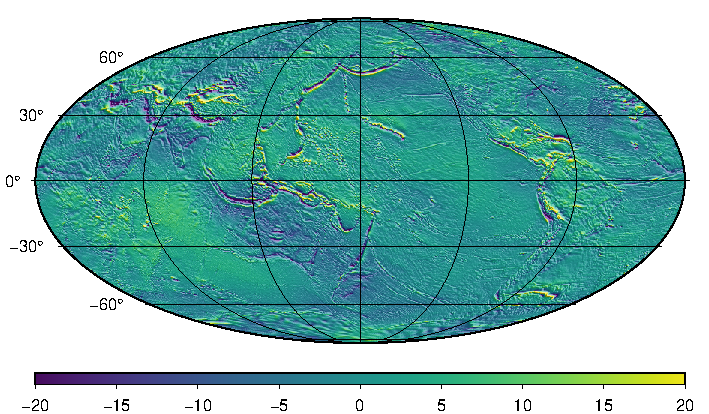
\includegraphics{./fig-deflections-xi.pdf}
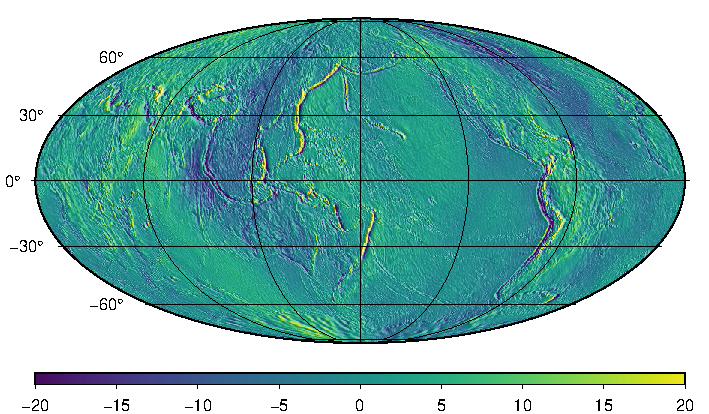
\includegraphics{./fig-deflections-eta.pdf}
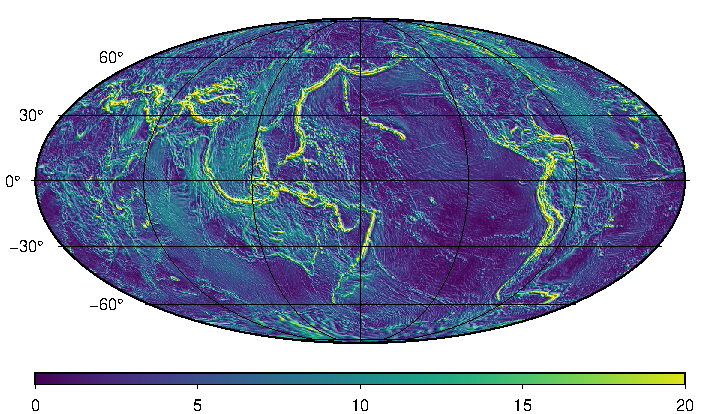
\includegraphics{./fig-deflections-theta.pdf}
\caption{Zložky zvislicovej odchýlky $\xi$ (vrchná mapa), $\eta$ (prostredná 
mapa) a celková zvislicová odchýlka~$\Theta$ (spodná mapa)~(jednotky~$''$) pre 
zemské gravitačné pole vypočítané vzťahmi~(\ref{eq:deflection_total}) 
a~(\ref{eq:deflection_grav_s_sph}) zo sférického harmonického modelu EIGEN-6C4 
do stupňa~720 na povrchu elipsoidu~GRS80.  Normálne tiažové pole je generované 
ekvipotenciálnym elipsoidom~GRS80.}
\label{fig:deflections_ggm}
\end{figure}

Z~Obrázku~\ref{fig:deflections_ggm} vidíme, že zvislicové odchýlky dosahujú 
hodnotu zväčša niekoľkých desiatok uhlových sekúnd a~len zriedkavo hodnoty 
väčšie ako uhlová minúta.  Najväčšie vychýlenie skutočnej tiažnice nastáva 
v~oblastiach, v~ktorých dochádza k~prudkej horizontálnej zmene skutočného 
tiažového potenciálu (resp. poruchového potenciálu), napríklad v~oblastiach 
pohorí či tektonických zlomov.  Toto pozorovanie možno vysvetliť horizontálnym 
deriváciami vo vzťahoch~(\ref{eq:deflection_grav_s_sph}).  Vidíme tiež výraznú 
podobnosť medzi vrchnými dvoma mapami poruchy tiažového zrýchlenia na 
Obrázku~\ref{fig:dg_ggm_grs80} a zvislicovej odchýlky na 
Obrázku~\ref{fig:deflections_ggm}.  Táto podobnosť je daná úzkou súvislosťou 
medzi horizontálnymi zložkami vektora poruchy tiažového zrýchlenia a~zložkami 
zvislicovej odchýlky (pozri vzťah~\ref{eq:deflection_grav_s_sph}).






% -----------------------------------------------------------------------------

\chapter{Geoid}
\label{sec:geoid}

Vráťme sa na chvíľu do úvodnej kapitoly, v~ktorej sme uviedli dva prístupy 
k~definícii tvaru Zeme.  V~zmysle prvej definície je tvar Zeme daný jej 
skutočným fyzickým povrchom, ktorý ale musí byť kvôli svojmu komplikovanému 
priebehu do istej miery vyhladený.  Určovaním takto chápaného tvaru Zeme a~jej 
vonkajšieho tiažového poľa sa zaoberá Molodenského teória 
\parencite{Molodensky1962,Borre2006,MoritzAdvancedGeodesy,MoritzPhysicalGeodesy}.  
V~druhom prístupe je tvar Zeme definovaný geoidom, teda ekvipotenciálnou 
plochou s~konštantným tiažovým potenciálom.  Na týchto stranách sa budeme 
bližšie zaoberať iba druhým spomínaným prístupom.\footnote{Pre predstavenie 
Molodenského teórie, pozri napríklad prácu~\textcite{Janak2006}.}

Z~Kapitol~\ref{sec:gravity_disturbance} až~\ref{sec:deflections} vieme, že 
medzi merateľné veličiny fyzikálnej geodézie patria najmä (no nielen) porucha 
tiažového zrýchlenia~$\delta g$, anomália tiažového zrýchlenia~$\Delta g$ 
a~zvislicové odchýlky~$\xi$, $\eta$.  Geoid preto určujeme spravidla z~týchto 
veličín.  Z~rovnice~(\ref{eq:N}) ďalej vieme, že na určenie výšky geoidu~$N$ 
nad referenčným elipsoidom (Obrázok~\ref{fig:geoid}) postačuje určiť poruchový 
potenciál na geoide~$T(P_0)$.\footnote{Normálne tiažové 
zrýchlenie~$\gamma(Q_0)$ vystupujúce v~rovnici~(\ref{eq:N}) môžeme vypočítať 
jednoducho Somiglianovým vzťahom~(\ref{eq:somigliana}).}  \emph{Linearizované} 
vzťahy medzi merateľnými veličinami fyzikálnej geodézie a~neznámym poruchovým 
potenciálom už poznáme (vzťahy~\ref{eq:dg_normals}, 
\ref{eq:Dg_fundamental_equation_earth}, 
\ref{eq:Dg_fundamental_equation_earth_sph}, \ref{eq:deflection_grav_nat}, 
\ref{eq:deflection_grav_e}, \ref{eq:deflection_grav_s}).  Je dobré si ale 
všimnúť, že v~týchto rovniciach síce vystupuje poruchový potenciál, ktorý 
potrebujeme určiť, ale vystupuje v~nich vo forme \emph{derivácie}, či už 
vertikálnej alebo horizontálnej.

Označme symbolmi~$\DIFF_{\Delta g}$ a~$\DIFF_{\delta g}$ \emph{diferenciálne 
operátory}, ktoré transformujú poruchový potenciál na veličinu, ktorá je 
uvedená v~dolnom indexe za symbolom~$\DIFF$.  Napríklad aplikácia 
diferenciálneho operátora
%
\begin{equation}
\label{eq:diff_Dg}
\DIFF_{\Delta g} = -\frac{\partial}{\partial r} - \frac{2}{r}
\end{equation}
%
na poruchový potenciál dáva sférickú aproximáciu anomálie tiažového zrýchlenia 
(porovnaj rovnice~\ref{eq:Dg_fundamental_equation_earth_sph} 
a~\ref{eq:diff_Dg}),
%
\begin{equation}
\Delta g = \DIFF_{\Delta g} T{.}
\end{equation}
%
Získame tak vzťahy
%
\begin{equation}
\label{eq:diff_operators}
\Delta g = \DIFF_{\Delta g}T{,} \quad \delta g = \DIFF_{\delta g}T{.}
\end{equation}
%
Aby sme dokázali vypočítať poruchový potenciál, na ktorý 
v~rovnici~(\ref{eq:diff_operators}) pôsobia diferenciálne operátory, 
potrebujeme nájsť \emph{integrálne operátory}~$\INT_{\Delta g}$ a~$\INT_{\delta 
g}$.  Tie aplikujeme na anomálie tiažového zrýchlenia~$\Delta g$ a~poruchy 
tiažového zrýchlenia~$\delta g$, čím získame hľadaný poruchový potenciál,
%
\begin{equation}
\label{eq:int_operators}
T = \INT_{\Delta g} \Delta g{,} \quad T = \INT_{\delta g}\delta g{.}
\end{equation}

Integrálne vzťahy~(\ref{eq:int_operators}) budeme hľadať pomocou okrajových 
úloh pre poruchový potenciál.  S~pojmom okrajová úloha sme sa už čiastočne 
stretli v~Kapitole~\ref{sec:u_boundary_value_problem} a~nepriamo aj 
v~Kapitole~\ref{sec:meaning_of_laplace_equation_in_practice}.  V~nasledujúcej 
Kapitole~\ref{sec:boundary_value_problem} najprv načrtneme princíp určovania 
poruchového potenciálu pomocou okrajových úloh.  
V~Kapitolách~\ref{sec:stokes_integral} až~\ref{sec:poisson_integral} potom 
popíšeme rôzne typy okrajových úloh, s~ktorými sa vo fyzikálnej geodézii často 
stretávame.  Pri čítaní týchto kapitol si všimnime, že vonkajšie tiažové pole 
Zeme určujeme, podobne ako v~Kapitole~\ref{sec:spherical_harmonic_expansion}, 
bez potreby priamej znalosti hustoty.  Okrajové úlohy budú totižto formulované 
tak, že informácia o~hustote Zeme bude zachytená vo vstupných anomáliách, 
resp. poruchách tiažového zrýchlenia (vzťahy~\ref{eq:int_operators}).  Tie 
v~praxi získavame gravimetrickým meraním veľkosti vektora tiažového zrýchlenia 
(Kapitola~\ref{sec:gravity_measurements}), ktoré túto informáciu implicitne 
obsahuje (Kapitola~\ref{sec:gg}).  Pripomeňme, že na získanie poruchového 
potenciálu sa sústredíme preto, lebo výpočet výšky geoidu nad referenčným 
elipsoidom zo známeho poruchového potenciálu je jednoduchý (vzťah~\ref{eq:N}).

K~výpočtu geoidu zo zvislicových odchýlok pristúpime iným spôsobom.  Zatiaľ čo 
poruchy a~anomálie tiažového zrýchlenia možno chápať skôr fyzikálne, pretože 
priamo súvisia s~\emph{veľkosťou} vektora tiažového zrýchlenia, zvislicové 
odchýlky možno vnímať geometricky (pozri Obrázok~\ref{fig:deflections}), 
pretože sú spojené so \emph{smerom} vektora tiažového zrýchlenia 
\parencite{MoritzPhysicalGeodesy}.  Na výpočet geoidu zo zvislicových odchýlok 
využijeme v~Kapitole~\ref{sec:geoid_astrogeodetic} práve geometrickú 
interpretáciu zvislicových odchýlok.

Následne v~Kapitole~\ref{sec:other_geoid_determination_methods} spomenieme 
ďalšie metódy určovania geoidu a~na záver v~Kapitole~\ref{sec:vm_integral} pre 
úplnosť uvedieme spôsob, ktorým možno vypočítať zvislicové odchýlky 
z~gravimetrických dát.


\section{Okrajová úloha pre poruchový potenciál}
\label{sec:boundary_value_problem}

Nech~$\Omega$ je vnútorná časť Zemského telesa a~$\partial \Omega$ nech je jeho 
povrch, v~tomto prípade geoid (Obrázok~\ref{fig:boundary_value_problems}).  
O~hranici~$\partial \Omega$ budeme predpokladať, že je dostatočne 
hladká.\footnote{Pozri napríklad prácu \textcite{SansoGeoidDetermination}.}  
Táto podmienka je splnená, pretože geoid je ekvipoteciálnou plochou, a~tak je 
hladký (Kapitola~\ref{sec:equipotential_surface}).  Symbolom $\overline{\Omega} 
= \Omega \cup \partial\Omega$ budeme označovať zemské teleso spolu s~jeho 
povrchom.  Ďalej, nech sa mimo telesa~$\overline{\Omega}$ nenachádzajú žiadne 
hmoty, teda napríklad ani nebeské telesá, ani zemská atmosféra či ani tá časť 
zemských hmôt, ktoré sa spravidla nachádzajú nad geoidom v~pevninskej časti 
zemského povrchu.  Túto vonkajšiu oblasť označme~$\mathbb{R}^3 
- \overline{\Omega}$.

\begin{figure}[bt]
\centering
\input{./fig-boundary-value-problems.pdf_tex}
\caption{Geometrické znázornenie oblastí vystupujúcich v~okrajovej úlohe pre 
poruchový potenciál Zeme.}
\label{fig:boundary_value_problems}
\end{figure}

Našim cieľom je nájsť vzťahy, ktoré by umožnili získať poruchový potenciál na 
hranici~$\partial \Omega$ a v~celej oblasti~$\mathbb{R}^3 - \overline{\Omega}$ 
z~poruchy tiažového zrýchlenia a~z~anomálie tiažového zrýchlenia, o~ktorých 
predpokladáme, že sú známe (odmerané) na hranici~$\partial \Omega$.  S trochou 
námahy nie je náročné uvedomiť si, že túto úlohu by nebolo možné vyriešiť bez 
toho, aby sme vedeli dostatočne veľa o~tom, ako sa samotný poruchový potenciál 
\emph{mení} vo vonkajšom priestore mimo hranice~$\partial\Omega$, na ktorej sú 
dostupné anomálie, resp. poruchy tiažového zrýchlenia.  Informáciu, ktorá 
popisuje túto zmenu poruchového potenciálu, zachytáva Laplaceova 
rovnica~(\ref{eq:laplace_xyz_t}).\footnote{Pre diskusiu o~význame Laplaceovej 
rovnice pre fyzikálnu geodéziu pozri 
Kapitolu~\ref{sec:meaning_of_laplace_equation_in_practice}.}  \emph{Okrajovou 
úlohou pre poruchový potenciál} teda rozumieme hľadanie takého riešenia 
diferenciálnej rovnice~(\ref{eq:laplace_xyz_t}), ktoré v~oblasti~$\mathbb{R}^3 
- \overline\Omega$ vyhovuje tejto rovnici a~na hranici~$\partial \Omega$ 
reprodukuje zadanú podmienku.  Podmienku zadanú na hranici~$\partial \Omega$ 
nazývame \emph{okrajová podmienka}.  Okrajová podmienka musí byť v~nejakom 
vzťahu voči hľadanému poruchovému potenciálu.  Ako okrajová podmienka tak môže 
byť na hranici~$\partial \Omega$ zadaná napríklad niektorá z~nasledovných 
veličín:
%
\begin{itemize}
\item lineárna kombinácia poruchového potenciálu~$T$ a~jeho prvej derivácie 
v~smere vonkajšej normály v~podobe anomálie tiažového zrýchlenia~$\DIFF_{\Delta 
g}T$ (rovnica~\ref{eq:Dg_fundamental_equation_earth_sph}) (táto okrajová 
podmienka sa zvykne nazývať \emph{Newtonova okrajová podmienka}; 
Kapitola~\ref{sec:stokes_integral}),
%
\item prvá derivácia poruchového potenciálu v~smere vonkajšej normály v~podobe 
poruchy tiažového zrýchlenia~$\DIFF_{\delta g} T$ (rovnica~\ref{eq:dg_normals}) 
(\emph{Neumannova okrajová podmienka}; Kapitola~\ref{sec:hotine_integral}),
%
\item samotný poruchový potenciál~$T$ (\emph{Dirichletova okrajová podmienka}; 
Kapitola~\ref{sec:poisson_integral}),
%
\item druhá vertikálna derivácia poruchového potenciálu~$\partial^2 
T / \partial r^2$ (táto okrajová úloha nie je predmetom tejto práce), atď.
\end{itemize}
%
V~praxi závisí voľba typu okrajovej podmienky najmä od typu dostupných dát.

Vzťahy~(\ref{eq:int_operators}) označujú všeobecný zápis riešenia získaného 
z~prvých dvoch uvedených okrajových úloh.  Na pravej strane týchto rovníc 
vystupujú okrajové podmienky na hranici~$\partial \Omega$ (odmerané vstupné 
dáta) a~na ľavej strane vystupuje hľadaný poruchový potenciál~$T$, ktorý možno 
vypočítať nielen na hranici~$\partial\Omega$ ale aj v~oblasti~$\mathbb{R}^3 
- \overline\Omega$.  Spomeňme, že poruchový potenciál získaný z~každej z~týchto 
okrajových úloh je, prirodzene, totožný, teda napríklad
%
\begin{equation}
T = \INT_{\Delta g} \Delta g = \INT_{\delta g}\delta g{.}
\end{equation}
%
Rozdielne sú iba okrajové podmienky, a~teda následne aj integrálne 
operátory~$\INT_{\Delta g}$ a~$\INT_{\delta g}$.


\subsubsection{Poznámka k~okrajovým a~počiatočným úlohám}

\emph{Okrajová úloha} je v~matematike všeobecný pojem, ktorý označuje riešenie 
diferenciálnej rovnice so zadanou okrajovou podmienkou.  Okrajová podmienka sa 
spravidla vzťahuje k~priestoru (napríklad povrch telesa).  Naproti tomu, pojmom 
\emph{počiatočná úloha} označujeme riešenie diferenciálnej rovnice so zadanou 
počiatočnou podmienkou.  Počiatočná podmienka sa zvyčajne vzťahuje k~časovému 
okamihu.  Počiatočné úlohy sa teda zaoberajú vývojom diferenciálnej rovnice 
v~čase.  Podrobnejšie informácie o~okrajových a~počiatočných úlohách, o~ich 
klasifikácii a~o~metódach ich riešenia je možné nájsť napríklad v~prácach 
\textcite{Janak2006} a~\textcite{Macak2021}.


\section{Stokesov integrál}
\label{sec:stokes_integral}

Definujme okrajovú úlohu pre poruchový potenciál s~využitím okrajovej podmienky 
vo forme sférickej aproximácie anomálie tiažového zrýchlenia:
%
\begin{alignat}{2}
\nabla^2 T(P) &= 0{,} &&P \in \mathbb{R}^3 
- \overline\Omega{,}\label{eq:bvp_Dg_laplace}\\
\Delta g(P) &= -\left.\frac{\partial T}{\partial r}\right|_P 
- \left.\frac{2}{r}\right|_P \, T(P){,} \quad &&P \in 
\partial\Omega{,}\label{eq:bvp_Dg_boundary_condition}\\
T &\rightarrow 0 &&\textrm{pre} \quad r \rightarrow 
\infty{.}\label{eq:bvp_Dg_t_infty}
\end{alignat}
%
Vzťah~(\ref{eq:bvp_Dg_laplace}) definuje diferenciálnu rovnicu, ktorá je 
predmetom riešenia okrajovej úlohy na oblasti~$\mathbb{R}^3 - \overline\Omega$.  
Rovnica~(\ref{eq:bvp_Dg_boundary_condition}) špecifikuje konkrétny typ 
okrajovej podmienky, ktorá platí na geoide~$\partial\Omega$.  
Vzťah~(\ref{eq:bvp_Dg_t_infty}) dodáva ďalšiu informáciu o~poruchovom 
potenciáli; hovorí, že s~narastajúcim sprievodičom~$r$ bodu~$P(r, \varphi, 
\lambda)$ od Zeme~$\overline\Omega$ sa poruchový potenciál~$T$ blíži k~nule 
(pozri tiež vzťah~\ref{eq:t_infty}).  
Bez~rovníc~(\ref{eq:bvp_Dg_boundary_condition}) a~(\ref{eq:bvp_Dg_t_infty}) by 
mala diferenciálna rovnica~(\ref{eq:bvp_Dg_laplace}) nekonečne veľa riešení.  
Toto tvrdenie možno jednoducho dokázať napríklad na funkcii~$c \slash l(P)$, 
kde~$c$ je reálna konštanta a~$l(P)$ je vzdialenosť bodu~$P$ od začiatku 
súradnicového systému, ktorý sa nachádza, povedzme, v~ťažisku 
Zeme~$\overline\Omega$.  Z~rovníc~(\ref{eq:nabla_l}) 
a~(\ref{eq:l_2nd_derivatives}) totižto vieme, že funkcia~$c \slash l(P)$ 
vyhovuje rovnici~(\ref{eq:bvp_Dg_laplace}) pre \emph{ľubovoľnú} reálnu 
konštantu~$c$ za predpokladu~$l(P) > 0$.  
Rovnice~(\ref{eq:bvp_Dg_boundary_condition}) a~(\ref{eq:bvp_Dg_t_infty}) tak 
zabezpečujú, že získame práve jedno riešenie rovnice~(\ref{eq:bvp_Dg_laplace}).  
Odvodenie riešenia okrajovej úlohy v~tejto práce vynecháme a~zameriame sa skôr 
na popis získanej rovnice.  Odvodenie je možné nájsť napríklad 
v~prácach~\textcite{MoritzPhysicalGeodesy} a~\textcite{Janak2006}.

Riešením okrajovej úlohy~(\ref{eq:bvp_Dg_laplace})~--~(\ref{eq:bvp_Dg_t_infty}) 
je vzťah
%
\begin{equation}
\label{eq:stokes}
T(P) = \frac{R}{4\pi} \, \iint\limits_{\sigma} S(P, P') \, \Delta g(P') \, 
\diff \sigma'{,} \quad P \in \mathbb{R}^3 - \overline\Omega{,} \quad P' \in 
\partial\Omega{,}
\end{equation}
%
ktorý sa nazýva \emph{Stokesov integrál}.  Symbol~$R$ označuje polomer 
referenčnej sféry Zeme (napríklad stredný či rovníkový polomer Zeme), $\sigma$ 
je jednotková sféra a~$\diff\sigma'$ je jej diferenciál,
%
\begin{equation}
\label{eq:diff_sigma}
\diff\sigma' = \cos\varphi' \, \diff\varphi' \, \diff\lambda'{,}
\end{equation}
%
$S$ je \emph{Stokesovo integračné jadro} (niekedy tiež nazývané Stokesova 
funkcia), $P(r, \varphi, \lambda)$ je bod, v~ktorom je počítaný poruchový 
potenciál, a~$P'(R, \varphi', \lambda')$ je bod na geoide 
(Obrázok~\ref{fig:surface_integral}).  Stokesovo integračné jadro~$S$ závisí 
iba od vzájomnej polohy bodov~$P$ a~$P'$ \parencite{MoritzPhysicalGeodesy},
%
\begin{equation}
\label{eq:stokes_kernel_general}
\begin{split}
S(P, P') &= S(\underbrace{r, \varphi, \lambda}_{P}, \underbrace{R, \varphi', 
\lambda'}_{P'}) = S(r, \psi)\\
%
&= \frac{2R}{l} + \frac{R}{r} - 3\frac{R \, l}{r^2} - \frac{R^2}{r^2} \, 
\cos\psi\left( 5 + 3 \, \ln \frac{r - R \, \cos\psi + l}{2 \, r} \right){,}
\end{split}
\end{equation}
%
kde~$l$ a~$\psi$ sú Euklidovská a~sférická vzdialenosť medzi bodmi~$P$ a~$P'$ 
(rovnice~\ref{eq:l_sph} a~\ref{eq:cospsi}).

\begin{figure}[bt]
\centering
\input{./fig-surface-integral.pdf_tex}
\caption{Výpočtový bod~$P(\varphi, \lambda)$ premietnutý na jednotkovú sféru 
a~diferenciálny integračný element~$\diff\sigma'$ na jednotkovej sfére.  
Symbol~$\psi$ označuje sférickú vzdialenosť medzi~$P$ a~$\diff\sigma'$ 
a~$\alpha$ označuje azimut spojnice~$P$ a~$\diff\sigma'$.}
\label{fig:surface_integral}
\end{figure}

Stokesov integrál~(\ref{eq:stokes}) umožňuje vypočítať poruchový potenciál 
kdekoľvek v~oblasti~$\mathbb{R}^3 - \overline\Omega$.  Osobitne zaujímavý je 
prípad, v~ktorom výpočtový bod leží na rovnakej sfére ako anomálie tiažového 
zrýchlenia, teda keď~$r = R$.  Všeobecný tvar Stokesovho 
jadra~(\ref{eq:stokes_kernel_general}) potom prejde do tvaru, ktorý závisí iba 
od sférickej vzdialenosti~$\psi$,
%
\begin{equation}
\label{eq:stokes_kernel}
\begin{split}
S(\psi) = \frac{1}{\sin\dfrac{\psi}{2}} - 6 \, \sin\frac{\psi}{2} + 1 - 5 \, 
\cos\psi - 3 \, \cos\psi \, \ln\left( \sin\frac{\psi}{2} + \sin^2\frac{\psi}{2} 
\right){.}
\end{split}
\end{equation}
%
Stokesov integrál sa v~taktomto prípade zvykne zapisovať v~zjednodušenej forme
%
\begin{equation}
\label{eq:stokes_simplified}
T = \frac{R}{4\pi} \, \iint\limits_{\sigma} S(\psi) \, \Delta g_0 \, \diff 
\sigma{,}
\end{equation}
%
pričom~$T = T(P)$, $P(R, \varphi, \lambda) \in \partial\Omega$, $\Delta g_0 
= \Delta g_0(P')$, $P'(R, \varphi', \lambda') \in \partial\Omega$ 
a~$\diff\sigma = \diff\sigma'$.  Symbol~$\Delta g_0$ označuje anomálie 
tiažového zrýchlenia na geoide (pozri Kapitolu~\ref{sec:gravity_anomaly}).

Dosadením rovnice~(\ref{eq:stokes_simplified}) do Brunsovho vzorca~(\ref{eq:N}) 
získame vzťah na výpočet výšky geoidu nad referenčným elipsoidom z~meraní 
tiažového zrýchlenia,
%
\begin{equation}
\label{eq:stokes_N}
N = \frac{R}{4\pi \, \gamma_0} \, \iint\limits_{\sigma} S(\psi) \, \Delta g_0 
\, \diff \sigma{,}
\end{equation}
%
kde $\gamma_0 = \gamma(Q_0)$.  Rovnica~(\ref{eq:stokes_N}) predstavuje jednu zo 
základných rovníc fyzikálnej geodézie.

Dodajme, že z~rovnice~(\ref{eq:stokes}) vyplýva tvar hľadaného integrálneho 
operátora~$\mathcal{I}_{\Delta g}$ z~rovnice~(\ref{eq:int_operators}),
%
\begin{equation}
\label{eq:iDg}
\mathcal{I}_{\Delta g}( \, \cdot \, )(P) = \frac{R}{4\pi} \, 
\iint\limits_\sigma S(P, P') ( \, \cdot \, )(P') \, \diff\sigma'{,}
\end{equation}
%
kde symbol $(\, \cdot \,)$ označuje funkciu, na ktorú je integrálny operátor 
aplikovaný.


\subsection{Stokesovo integračné jadro}
\label{sec:stokes_kernel}

Význam Stokesovej funkcie vo vzťahu~(\ref{eq:stokes}) lepšie pochopíme po 
grafickom znázornení jej priebehu (Obrázok~\ref{fig:stokes_kernel}).  Z~obrázku 
a~z~rovnice~(\ref{eq:stokes_kernel}) je zrejmé, hodnota Stokesovej funkcie 
klesá so zväčšujúcou sa sférickou vzdialenosťou~$\psi$ až po vzdialenosť~$\psi 
\approx 72^\circ$, po ktorej začína mierne stúpať s~narastajúcim~$\psi$.  
V~súvislosti s~rovnicou~(\ref{eq:stokes}) to znamená, že na hodnotu poruchového 
potenciálu~$T(P)$ majú najväčší vplyv anomálie tiažového zrýchlenia~$\Delta 
g(P')$, ktoré sa nachádzajú v~blízkosti výpočtového bodu~$P$.  Inými slovami, 
anomálie tiažového zrýchlenia~$\Delta g(P')$ v~blízkom okolí výpočtového bodu 
sú v~rovnici~(\ref{eq:stokes}) násobené (\emph{vážené}) väčšími hodnotami 
Stokesovej funkcie~$S$ ako tie anomálie, ktoré sa nachádzajú ďaleko od 
výpočtového bodu; ich relatívny prínos do hodnoty poruchového potenciálu je tak 
väčší ako v~prípade veľkých vzdialeností medzi~$P$ a~$\diff\sigma'$.  Na 
Obrázku~\ref{fig:stokes_kernel} tiež vidíme, že Stokesovo integračné jadro 
nadobúda nulové hodnoty pre sférické vzdialenosti približne~$39^\circ$ 
a~$117^\circ$ \parencite{TorgeGeodesy}.  Príspevok anomálií tiažového, ktoré sa 
nachádzajú v~týchto vzdialenostiach voči výpočtovému bodu, je preto nulový.

\begin{figure}[bt]
\centering
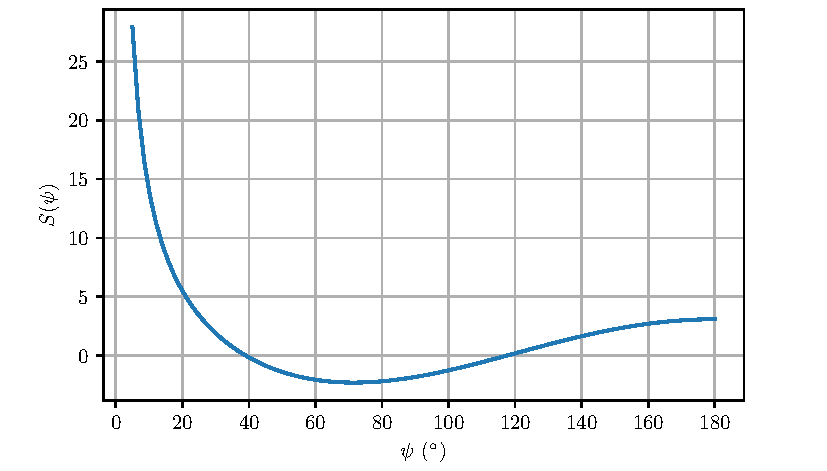
\includegraphics{./fig-stokes-kernel.pdf}
\caption{Stokesova funkcia~$S(\psi)$ (vzťah~\ref{eq:stokes_kernel}) na 
intervale~$[5^\circ, 180^\circ]$.}
\label{fig:stokes_kernel}
\end{figure}

Stokesova funkcia má niekoľko ďalších zaujímavých vlastností.
%
\begin{itemize}
\item \emph{Singularita}.  Pre~$P(r, \varphi, \lambda) \rightarrow P'(R, 
\varphi', \lambda')$ sa hodnota Stokesovej funkcie blíži k~nekonečnu (pre pojem 
singularita pozri tiež Kapitolu~\ref{sec:spheroidal_harmonics}),
%
\begin{equation}
\label{eq:stokes_singularity}
\lim\limits_{P \rightarrow P'} S(P, P') = \infty{.}
\end{equation}
%
K~singularite Stokesovej funkcie dochádza vtedy, keď integrál~(\ref{eq:stokes}) 
je počítaný na tej sfére, na ktorej je zadaná okrajová podmienka v~podobe 
anomálií tiažového zrýchlenia, teda ak~$r = R$ a~súčasne~$P(r, \varphi, 
\lambda) = P'(R, \varphi', \lambda')$.  Napriek 
vlastnosti~(\ref{eq:stokes_singularity}) však bude výsledok 
integrácie~(\ref{eq:stokes}), teda poruchový potenciál v~bode~$P$, nadobúdať 
\emph{konečnú} hodnotu (pre podobnú situáciu v~súvislosti s~Newtonovým 
integrálom pozri tiež diskusiu zo záveru Kapitoly~\ref{sec:potential_theory}).  
V~numerických výpočtoch je ale i~tak potrebné venovať osobitnú pozornosť 
prípadu, v~ktorom sú výpočtový bod a~stred integračného elementu totožné, 
a~použiť vhodné matematické úpravy (pozri napríklad 
\cite{MoritzPhysicalGeodesy} či \cite{Hees1991}).  Dodajme, že vo všeobecnosti 
neplatí, že každé singulárne integračné jadro vedie ku konečným hodnotám 
integrálu.  To, či je hodnota integrálu konečná alebo nie, závisí od typu 
singularity.
%
\item \emph{Homogénnosť}.  Hodnota Stokesovho integračného jadra nezávisí od 
polohy bodov~$P$ a~$P'$ v~priestore za predpokladu, že $r$ a~$\psi$ ostávajú 
nezmenené.  Ak sa napríklad body~$P$ a~$P'$ nachádzajú na tej istej sfére a~na 
tom istom meridiáne, hodnota Stokesovej funkcie~$S(\psi)$ je rovnaká bez ohľadu 
na to, v~ktorej časti meridiánu a~na ktorom meridiáne sa body~$P$ a~$P'$ 
nachádzajú, pokiaľ ich vzdialenosť~$\psi$ ostáva nezmenená.
%
\item \emph{Izotropnosť}.  Hodnota Stokesovho integračného jadra nezávisí od 
azimutu~$\alpha$ spojnice bodov~$P$ a~$P'$ (pozri 
Obrázok~\ref{fig:surface_integral}).
\end{itemize}

Stokesovu funkciu je možné vyjadriť aj ekvivalentným spôsobom pomocou rozvoja 
do radu Legendreových polynómov \parencite{MoritzPhysicalGeodesy},
%
\begin{equation}
\label{eq:stokes_spectral}
S(r, \psi) = \sum_{n = 2}^{\infty} \frac{2n + 1}{n - 1} \, \left( \frac{R}{r} 
\right)^{n + 1} \, P_n(\cos\psi){.}
\end{equation}
%
Rovnice~(\ref{eq:stokes_kernel_general}) a~(\ref{eq:stokes_kernel}) nazývame 
\emph{priestorový tvar} Stokesovho integračného jadra.  
Vzťah~(\ref{eq:stokes_spectral}) nazývame \emph{spektrálny tvar} Stokesovho 
integračného jadra.  To, ktorý tvar je výhodnejšie použiť, často závisí od 
aplikácie.  Ak anomálie tiažového zrýchlenia~$\Delta g$ nachádzajúce sa 
v~integráli~(\ref{eq:stokes}) boli získané meraním, môže byť vhodnejšie použiť 
priestorový tvar.  Je tomu tak preto, lebo odmerané gravitačné, resp. tiažové 
zrýchlenie zahŕňa vplyv všetkých harmonických stupňov (pozri nekonečné sumácie 
vo vzťahoch~\ref{eq:vgx_sh}, \ref{eq:vgy_sh} a~\ref{eq:vgz_sh}), rovnako tak 
ako priestorový tvar Stokesovho jadra~(\ref{eq:stokes_kernel_general}) 
implicitne obsahuje všetky harmonické stupne zo spektrálneho 
tvaru~(\ref{eq:stokes_spectral}) (pravá strana 
rovnice~\ref{eq:stokes_kernel_general} sa rovná pravej strane 
rovnice~\ref{eq:stokes_spectral}).  Výpočet Stokesovho jadra spektrálnym tvarom 
by bol v~tejto situácii nevhodný, pretože nekonečný rad by musel byť 
v~praktickom výpočte obmedzený na konečný počet členov, čo by spôsobilo 
aproximačné chyby.  Ak ale boli anomálie tiažového zrýchlenia~$\Delta g$ 
vypočítané z~konečného sférického harmonického radu vzťahom~(\ref{eq:Dg_sh_sa}) 
do stupňa~$N$, potom môže byť výhodnejšie použiť spektrálny 
tvar~(\ref{eq:stokes_spectral}) rozvinutý do identického maximálneho 
stupňa~$N$.\footnote{Z~teoretického hľadiska môže byť ekvivalentne použitý aj 
priestorový tvar Stokesovho jadra, prípadne jeho spektrálny tvar, ktorý je 
rozvinutý do vyššieho stupňa ako~$N$ \parencite[pozri 
napríklad][]{Freeden2009}.}

Všimnime si, že vo vzťahoch~(\ref{eq:stokes_kernel_general}), 
(\ref{eq:stokes_kernel}) a~(\ref{eq:stokes_spectral}) sa \emph{nenachádza} 
vplyv nultého harmonického stupňa (sumácia v~rovnici~\ref{eq:stokes_spectral} 
začína od stupňa~$2$ a~pravé strany týchto rovníc sú si rovné).  S~uvážením 
nultého harmonického stupňa má Stokesovo integračné jadro nasledovný tvar,
%
\begin{align}
S(r, \psi) &= \frac{2R}{l} - 3\frac{R \, l}{r^2} - \frac{R^2}{r^2} \, 
\cos\psi\left( 5 + 3 \, \ln \frac{r - R \, \cos\psi + l}{2 \, r} \right){,}
\label{eq:stokes_kernel_general_n0}
\\
%
S(\psi) &= \frac{1}{\sin\dfrac{\psi}{2}} - 6 \, \sin\frac{\psi}{2} - 5 \, 
\cos\psi - 3 \, \cos\psi \, \ln\left( \sin\frac{\psi}{2} + \sin^2\frac{\psi}{2} 
\right){,}
\label{eq:stokes_kernel_n0}
\\
%
S(r, \psi) &= \sum_{n = 0{,}\, n \neq 1}^{\infty} \frac{2n + 1}{n - 1} \, 
\left( \frac{R}{r} \right)^{n + 1} \, P_n(\cos\psi){.}
\label{eq:stokes_spectral_n0}
\end{align}
%
Tieto tvary je potrebné použiť vtedy, keď anomálie tiažového zrýchlenia vo 
vzťahu~(\ref{eq:stokes}) obsahujú aj vplyv nultého harmonického člena 
z~rovnice~(\ref{eq:Dg_sh_sa}).  Všimnime si tiež, že stupeň~$n$ 
v~rovnici~(\ref{eq:stokes_spectral_n0}) nesmie byť rovný~$1$ (aby bolo 
zamedzené deleniu nulou), čo je v~súlade s~anomáliami tiažového zrýchlenia, 
pretože na ne nevplýva harmonický stupeň~$n = 1$ (pozri poznámku 
k~rovnici~\ref{eq:Dg_sh_sa}).


\subsection{Stokesov integrál ako konvolučný integrál}
\label{sec:stokes_convolution}

Výpočtom integrálu na pravej strane rovnice~(\ref{eq:stokes}) získame poruchový 
potenciál v~bode~$P$, teda jedno číslo.  Ak chceme získať poruchový potenciál 
v~ďalšom bode~$P_1$, integráciu je potrebné zopakovať s~novým výpočtovým 
bodom~$P_1$.  Dôvod je ten, že hoci anomálie tiažového zrýchlenia~$\Delta 
g(P')$ sú identické (daná funkcia na hranici~$\partial\Omega$), zmena polohy 
výpočtového bodu z~$P$ na~$P_1$ spôsobí, že nové Stokesovo integračné 
jadro~$S(P_1, P')$ bude vážiť tie isté anomálie tiažového zrýchlenia~$\Delta 
g(P')$ iným spôsobom ako predošlé integračné jadro~$S(P, P')$.  Ak teda chceme 
získať poruchový potenciál~$P$ v~každom bode na Zemi, výpočtový bod~$P$ je 
potrebné vnímať ako premennú a~integráciu opakovať, vždy s~iným výpočtovým 
bodom.  Výsledkom tohto procesu bude nová funkcia, ktorou je poruchový 
potenciál na celej sfére.  Matematická operácia, ktorá transformuje dve funkcie 
na tretiu funkciu sa nazýva \emph{konvolúcia}.  V~našom prípade konvolúciou 
transformujeme Stokesovo integračné jadro~$S$ a~anomálie tiažového 
zrýchlenia~$\Delta g$ na poruchový potenciál~$T$.  Symbolicky túto operáciu 
zapíšeme nasledovne,
%
\begin{equation}
\label{eq:stokes_convolution}
\frac{R}{4 \, \pi}(S * \Delta g)(P) = \frac{R}{4\pi} \, \iint\limits_\sigma 
S(P, P') \, \Delta g(P') \, \diff\sigma'{,}
\end{equation}
%
kde symbol~$*$ označuje konvolučné násobenie funkcií~$S$ a~$\Delta g$.

S~konvolučnými integrálmi sa vo fyzikálnej geodézii stretávame veľmi často.  
Konvolučným integrálom je napríklad aj samotný Newtonov 
integrál~(\ref{eq:vg_body}) a~ďalšie integrály, ktoré sú z~neho odvodené 
(napríklad integrál~\ref{eq:gg_body}).  Vo vzťahu~(\ref{eq:vg_body}) hrá 
hustota~$\rho$ podobnú úlohu ako anomálie tiažového zrýchlenia~$\Delta g$ vo 
vzťahu~(\ref{eq:stokes}), a~prevrátená hodnota vzdialenosti~$1 \slash l$ 
predstavuje integračné jadro.  Všimnime si, že vo vzťahu~(\ref{eq:gg_body}) 
vystupuje v~úlohe meraných dát tá istá hustota ako 
v~rovnici~(\ref{eq:vg_body}); keďže ale vzťah medzi gravitačným zrýchlením 
z~rovnice~(\ref{eq:gg_body}) a~hustotou je iný ako vzťah medzi gravitačným 
potenciálom (\ref{eq:vg_body}) a~hustotou, konvolučné jadro, $\vec r \slash 
l^3$, je tentokrát iné ako v~rovnici~(\ref{eq:vg_body}).  Rozličné integračné 
jadrá teda transformujú tú istú funkciu rozdielne.

Konvolučné integrály sa vyskytujú v~mnohých oblasti matematiky, fyziky 
a~ďalších vedných disciplínach.  Jedno z~množstva využití konvolúcie je na 
potlačenie šumu na zvukových nahrávkach.  Vstupný signál, teda pôvodná 
nahrávka, je konvolučne vynásobený vhodným integračným jadrom, výsledkom čoho 
je upravená nahrávka s~potlačeným šumom, teda výstupný signál 
(Obrázok~\ref{fig:convolution}).  Aplikáciou iného konvolučného jadra na tú 
istú nahrávku môžeme napríklad zvýrazniť istú časť spektra na nahrávke, 
povedzme nízke frekvencie a~pod.  Pre konvolučné integrály je typické, že ich 
numerický výpočet je časovo veľmi náročný.  Snahou preto je použiť efektívne 
algoritmy, napríklad rýchlu Fourierovu transformáciu 
\parencite[napríklad][]{PressNumericalRecipes} či vlnkovú transformáciu 
\parencite[napríklad][]{KellerWavelets}.  Obe transformácie sa používajú aj na 
efektívny výpočet konvolučných integrálov fyzikálnej geodézie \parencite[pozri 
napríklad][]{Forsberg1984,Freeden1998a,SansoGeoidDetermination}.

\begin{figure}[bt]
\centering
\input{./fig-convolution.pdf_tex}
\caption{Konvolúcia z~pohľadu spracovania signálu.  \textit{Vstupný signál} je 
konvolučným násobením transformovaný na \textit{výstupný signál}.}
\label{fig:convolution}
\end{figure}


\subsection{Sférická aproximácia v~Stokesovom integráli}
\label{sec:stokes_spherical_approximation}

Riešenie~(\ref{eq:stokes}) okrajovej úlohy~(\ref{eq:bvp_Dg_laplace})~-- 
(\ref{eq:bvp_Dg_t_infty}) bolo získané s~využitím sférickej aproximácie.  
Sférická aproximácia bola použitá jednak v~definícii okrajovej 
podmienky~(\ref{eq:bvp_Dg_boundary_condition}), ale tiež v~riešení okrajovej 
úlohy, čo má niekoľko dôsledkov pre praktické určovanie geoidu 
vzťahom~(\ref{eq:stokes_N}).  Hoci získané riešenie~(\ref{eq:stokes}) využíva 
anomálie tiažového zrýchlenia na geoide~$\Delta g_0$, samotná integrácia sa 
nevykonáva na geoide, ktorý má komplikovaný tvar, ale na sfére s~polomerom~$R$, 
ktorá geoid aproximuje.  Neznamená to však, že výšky geoidu získané 
vzťahom~(\ref{eq:stokes_N}) sú vztiahnuté k~referenčnej sfére s~polomer~$R$.  
Naopak, vzťahujú sa k~použitému ekvipotenciálnemu elipsoidu, preto aj normálne 
tiažové zrýchlenie~$\gamma_0$ v~rovnici~(\ref{eq:stokes_N}) má byť počítané 
Somiglianovým vzťahom pre ekvipotenciálny elipsoid 
(rovnica~\ref{eq:somigliana}).

Sférická aproximácia spôsobuje relatívnu chybu v~určení geoidu na úrovni~$3 
\times 10^{-3} N$, teda dosahuje hodnoty menšie ako 1~m 
\parencite{MoritzPhysicalGeodesy}.  Pre spresnenie riešenia je potrebné zaviesť 
korekciu zo sploštenia referenčného elipsoidu \parencite[pozri 
napríklad][]{Claessens2006}, prípadne integrovať priamo na ekvipotenciálnom 
elipsoide \parencite{Martinec1997}.


\section{Hotineov integrál}
\label{sec:hotine_integral}

Definujme teraz takú okrajovú úlohu, ktorá umožní vypočítať poruchový 
potenciál, a~teda geoid, z~porúch tiažového zrýchlenia vo sférickej 
aproximácii:
%
\begin{alignat}{2}
\nabla^2 T(P) &= 0{,} &&P \in \mathbb{R}^3 
- \overline\Omega{,}\label{eq:bvp_dg_laplace}\\
\delta g(P) &= -\left.\frac{\partial T}{\partial r}\right|_P{,} \quad &&P \in 
\partial\Omega{,}\label{eq:bvp_dg_boundary_condition}\\
T &\rightarrow 0 &&\textrm{pre} \quad r \rightarrow 
\infty{.}\label{eq:bvp_dg_t_infty}
\end{alignat}

Riešením okrajovej úlohy~(\ref{eq:bvp_dg_laplace})~-- 
(\ref{eq:bvp_dg_t_infty}), ktoré je možné nájsť napríklad v~prácach 
\textcite{MoritzPhysicalGeodesy} či \textcite{SansoGeoidDetermination}, získame 
rovnicu
%
\begin{equation}
\label{eq:hotine}
T(P) = \frac{R}{4\pi} \, \iint\limits_{\sigma} H(P, P') \, \delta g(P') \, 
\diff \sigma'{,} \quad P \in \mathbb{R}^3 - \overline\Omega{,} \quad P' \in 
\partial\Omega{.}
\end{equation}
%
Vzťah~(\ref{eq:hotine}) sa nazýva \emph{Hotineov integrál}.  Funkcia~$H$ sa 
nazýva \emph{Hotineovo integračné jadro} a~jej všeobecný tvar je daný vzťahom 
\parencite{SansoGeoidDetermination}
%
\begin{equation}
\label{eq:hotine_kernel_general}
H(P, P') = H(r, \psi) = \frac{2R}{l} - \ln\left(\frac{l + R - r \, \cos\psi}{r 
\, (1 - \cos\psi)}\right){,}
\end{equation}
%
ktorý sa pre~$r = R$ zjednoduší do tvaru (Obrázok~\ref{fig:hotine_kernel})
%
\begin{equation}
\label{eq:hotine_kernel}
H(\psi) = \frac{1}{\sin\dfrac{\psi}{2}} - \ln\left( 
1 + \frac{1}{\sin\dfrac{\psi}{2}} \right){.}
\end{equation}
%
Spektrálna reprezentácia Hotineovho jadra je daná vzťahom
%
\begin{equation}
\label{eq:hotine_spectral}
H(r, \psi) = \sum_{n = 0}^{\infty} \frac{2n + 1}{n + 1} \, \left( \frac{R}{r} 
\right)^{n + 1} \, P_n(\cos\psi){.}
\end{equation}
%
Podobne ako Stokesov integrál, aj Hotineov integrál~(\ref{eq:hotine}) patrí 
medzi konvolučné integrály (Kapitola~\ref{sec:stokes_convolution}) a~bol 
získaný vo sférickej aproximácii 
(Kapitola~\ref{sec:stokes_spherical_approximation}).  Hľadaný tvar integrálneho 
operátora~$\mathcal{I}_{\delta g}$ z~rovnice~(\ref{eq:int_operators}) je zrejmý 
z~porovnania rovníc~(\ref{eq:stokes}), (\ref{eq:hotine}) a~(\ref{eq:iDg}).

\begin{figure}[bt]
\centering
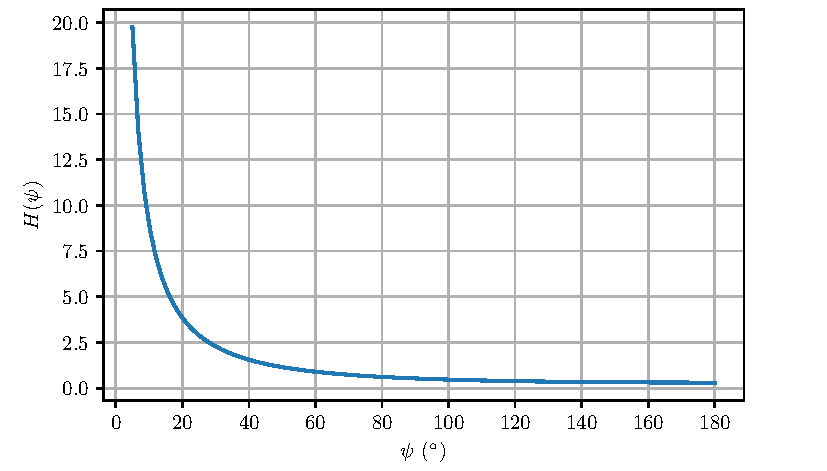
\includegraphics{./fig-hotine-kernel.pdf}
\caption{Hotineova funkcia~$H(\psi)$ (vzťah~\ref{eq:hotine_kernel}) na 
intervale~$[5^\circ, 180^\circ]$.}
\label{fig:hotine_kernel}
\end{figure}

Hotineovo integračné jadro má podobné vlastnosti ako Stokesovo integračné jadro 
(pozri Kapitolu~\ref{sec:stokes_kernel}), teda je singulárne, homogénne 
a izotropne.  Na rozdiel od Stokesovho jadra ale ide o~monotónne klesajúcu 
funkciu.  Teda čím ďalej sa nachádza integračný element $\diff\sigma'$ od 
výpočtového bodu~$P$, tým menšia váha~$H$ v~Hotineovom 
integráli~(\ref{eq:hotine}) je pridelená príslušnej poruche tiažového 
zrýchlenia.

Dosadením vzťahu~(\ref{eq:hotine}) pre~$P \in \partial\Omega$ do Brunsovho 
vzorca~(\ref{eq:N}) získame vzťah na výpočet geoidu z~porúch tiažového 
zrýchlenia,
%
\begin{equation}
\label{eq:hotine_N}
N = \frac{R}{4\pi \, \gamma_0} \, \iint\limits_{\sigma} H(\psi) \, \delta g_0 
\, \diff \sigma{,}
\end{equation}
%
kde symbol~$\delta g_0$ označuje poruchy tiažového zrýchlenia na geoide~$\delta 
g(P_0)$.  Vzťah~(\ref{eq:hotine_N}) možno bezpochyby zaradiť medzi 
najdôležitejšie vzťahy fyzikálnej geodézie.

M.~Hotine (1898~-- 1968) bol anglický geodet.  Jeho kniha \textit{Matematická 
geodézia} z~roku 1969 patrí medzi fundamentálne geodetické práce.

\section{Poissonov integrál}
\label{sec:poisson_integral}

Posledná geodetická okrajová úloha, ktorú v~tejto práci spomenieme, je okrajová 
úloha pre poruchový potenciál so zadanou okrajovou podmienkou vo forme 
poruchového potenciálu:
%
\begin{alignat}{2}
\nabla^2 T(P) &= 0{,} &&P \in \mathbb{R}^3 
- \overline\Omega{,}\label{eq:bvp_t_laplace}\\
T(P) &= f(P){,} \quad &&P \in 
\partial\Omega{,}\label{eq:bvp_t_boundary_condition}\\
T &\rightarrow 0 &&\textrm{pre} \quad r \rightarrow 
\infty{,}\label{eq:bvp_t_t_infty}
\end{alignat}
%
kde~$f$ predstavuje funkciu zadanú na hranici~$\partial\Omega$, v~tomto prípade 
samotný poruchový potenciál.

Riešenie tejto okrajovej úlohy \parencite[pre odvodenie pozri 
napríklad][]{MoritzPhysicalGeodesy,SansoGeoidDetermination} má tvar
%
\begin{equation}
\label{eq:poisson}
T(P) = \frac{R}{4\pi} \, \iint\limits_\sigma \Pi(P, P') \, T(P') \, 
\diff\sigma'
\end{equation}
%
a~nazýva sa \emph{Poissonov integrál}.  Symbol~$\Pi$ označuje Poissonovo 
integračné jadro,
%
\begin{align}
\Pi(r, \psi) &= \frac{r^2 - R^2}{l^3}{,}\label{eq:poisson_kernel}\\
\Pi(r, \psi) &= \sum_{n = 0}^{\infty} (2n + 1) \, \left( \frac{R}{r} \right)^{n 
+ 1} \, P_n(\cos\psi)\label{eq:poisson_kernel_spectral}{.}
\end{align}
%
Podobne ako v~predošlých Kapitolách~\ref{sec:stokes_integral} 
a~\ref{sec:hotine_integral}, Poissonovo jadro je singulárne, homogénne 
a izotropne a~Poissonov integrál je konvolučný.  Vyobrazenie Poissonovho jadra 
vynecháme, pretože pre fixnú hodnotu sprievodiča~$r$ ide o~známu funkciu~$c 
\slash l^3$, kde $c = r^2 - R^2$.

Poissonov integrál umožňuje získať akúkoľvek harmonickú funkciu v~celom 
priestore~$\mathbb{R}^3 - \overline\Omega$ z~hodnôt tejto funkcie na 
hranici~$\partial\Omega$.  Z~Kapitoly~\ref{sec:harmonic_function} vieme, že 
tento proces sa niekedy nazýva analytické pokračovanie, v~tomto prípade tiež 
\emph{harmonické pokračovanie}, pretože funkcia~$T$ vystupujúca v~Poissonovom 
integráli musí byť harmonická.  Poissonov integrál sa často používa aj 
inverzným spôsobom na pokračovanie nadol, hoci táto úloha je vo všeobecnosti 
nestabilná \parencite{SansoGeodeticBoundaryValueProblem}.  Okrem poruchového 
potenciálu je možné aplikovať Poissonov integrál aj na ďalšie harmonické 
funkcie, napríklad gravitačný potenciál~$V$ či funkciu~$r \, \Delta g$, ktorá 
je taktiež harmonická (samotná funkcia~$\Delta g$ však harmonická nie je).  
Poissonov integrál teda umožňuje riešiť mnohé kľúčové úlohy fyzikálnej 
geodézie.  Priamo na výpočet geoidu sa nezvykne používať, pretože predpokladá 
dostupnosť poruchového potenciálu na geoide.  Ak by bol ale poruchový potenciál 
na geoide známy, mohol by byť priamo použitý v~Brunsovom vzorci~(\ref{eq:N}) 
bez potreby formulovania a~riešenia okrajovej úlohy.




\section{Astronomicko--geodetická metóda určenia geoidu}
\label{sec:geoid_astrogeodetic}

Astronomicko--geodetická metóda určuje geoid zo sklonu geoidu voči 
ekvipotenciálnemu elipsoidu.  Tento sklon je popísaný Pizzettiho zvislicovou 
odchýlkou (Obrázok~\ref{fig:deflections}), ktorej priemet do spojnice dvoch 
bodov budeme v~tejto kapitole označovať symbolom~$\varepsilon_0$ bez horného 
indexu.  Dolný index indikuje, že zvislicová odchýlka sa vzťahuje ku geoidu.

\begin{figure}[bt]
\centering
\input{./fig-astrogeodetic-method.pdf_tex}
\caption{Astronomicko--geodetická metóda určenia geoidu.}
\label{fig:astrogeodetic_method}
\end{figure}

Na~Obrázku~\ref{fig:astrogeodetic_method} vidíme, že diferenciálne prevýšenie 
geoidu medzi bodmi~$A$ a~$B$ je dané vzťahom \parencite{MoritzPhysicalGeodesy}
%
\begin{equation}
\label{eq:N_deflections}
\diff N = -\varepsilon_0 \, \diff s{,}
\end{equation}
%
kde $\varepsilon_0$ je priemet zvislicovej odchýlky do spojnice bodov~$A$, $B$ 
(vzťah~\ref{eq:deflection_vareps}).  Znamienko mínus je konvenčne dohodnuté, 
podobne ako sme konvenčne použili v~rovnici~(\ref{eq:deflection_eps}) vektory 
vonkajších normál~$\vec n_W$, $\vec n_U$ a~nie vektory vnútorných normál~$-\vec 
n_W$, $-\vec n_U$.  Integráciou rovnice od bodu~$A$ po bod~$B$ získame výšku 
geoidu v~bode~$B$,
%
\begin{equation}
\label{eq:N_deflections_nb}
N_B = N_A - \int\limits_A^B \varepsilon_0 \, \diff s{,}
\end{equation}
%
pričom~$\varepsilon_0$ sa pozdĺž spojnice môže meniť.  Astronomicko--geodetická 
metóda určenia geoidu je teda \emph{relatívna} metóda, ktorou určujeme 
\emph{prevýšenie geoidu} medzi dvoma bodmi,
%
\begin{equation}
\label{eq:N_deflections_delta}
\Delta N_{AB} = N_B - N_A = - \int\limits_A^B \varepsilon_0 \, \diff s{.}
\end{equation}

V~praktických aplikáciách zvislicová odchýlka~$\varepsilon_0$ nie je známa 
\emph{spojito} pozdĺž spojnice bodov~$A$ a~$B$, tak ako to vyžaduje 
vzťah~(\ref{eq:N_deflections_delta}), ale len \emph{diskrétne}, zväčša 
v~koncových bodoch spojnice.  Integrál~(\ref{eq:N_deflections_delta}) preto 
vypočítame \emph{numerickou integráciou}, v~ktorej spojitú 
funkciu~$\varepsilon_0$ a~diferenciálne vzdialenosti~$\diff s$ nahradíme 
diskrétnymi hodnotami~$\varepsilon_{0,i}$ a~konečnými dĺžkami~$\Delta s_i$.  
Spravidla sú k~dispozícii zvislicové odchýlky~$\varepsilon_{0,A}$ 
a~$\varepsilon_{0,B}$ na koncových bodoch spojnice a~vzdialenosť~$\Delta 
s_{AB}$ medzi bodmi~$A$, $B$.  Obdĺžnikovou metódou získame prevýšenie geoidu 
medzi bodmi~$A$ a~$B$ \parencite[pre popis obdĺžnikovej metódy pozri 
napríklad][]{Macak2021},
%
\begin{equation}
\label{eq:N_deflections_delta_ni}
\Delta N_{AB} = -\frac{\varepsilon_{0,A} + \varepsilon_{0,B}}{2} \, \Delta 
s_{AB}{.}
\end{equation}
%
Prirodzene, čím je zložitejší priebeh geoidu medzi bodmi $A$ a~$B$, tým väčšej 
chyby sa dopúšťame použitím numerickej integrácie.  V~takom prípade je 
potrebné, pokiaľ je to možné, skrátiť vzdialenosti medzi bodmi siete.

Ak je geoid určovaný na viacerých bodoch, zvyčajne sa z~bodov vytvorí 
trojuholníková sieť a~vzťahom~(\ref{eq:N_deflections_delta_ni}) sa vypočítajú 
prevýšenia geoidu medzi bodmi siete.  V~dôsledku chýb meraní a~v~dôsledku 
použitia numerickej integrácie však spravidla nebude súčet prevýšení 
v~trojuholníkoch siete nulový.  Prevýšenia sa preto vyrovnajú metódou 
najmenších štvorcov tak, aby súčet prevýšení v~každom trojuholníku bol nulový.  
Na záver je potrebné odhadnuté prevýšenia geoidu pripojiť na jeden bod, 
v~ktorom je známa absolútna výška geoidu nad referenčným elipsoidom.

Dodajme, že geoid, môže byť vypočítaný zo zvislicových odchýlok aj integrálnymi 
vzťahmi, ktoré majú podobný charakter ako Stokesov a~Hotineov integrál 
\parencite[pozri napríklad][]{Sjoberg2017}.


\section{Ďalšie metódy určovania geoidu}
\label{sec:other_geoid_determination_methods}

\subsection{Numerické riešenie geodetických okrajových úloh}

V~Kapitolách~\ref{sec:stokes_integral} až~\ref{sec:poisson_integral} sme 
načrtli určovanie geoidu a~vonkajšieho tiažového poľa Zeme riešením okrajových 
úloh.  Získané riešenia (rovnice~\ref{eq:stokes}, \ref{eq:hotine} 
a~\ref{eq:poisson}) sa nazývajú \emph{analytické riešenia}.  Analytickým 
riešením rozumieme presný tvar hľadaného riešenia v~podobe funkcie, ktorá 
vyhovuje definícii okrajovej úlohy.  Okrajové úlohy sme si ale zjednodušili 
využím konceptu sférickej aproximácie, ktorá predpokladá okrajovú podmienku na 
sfére, nie na geoide.  V~presnejšom priblížení je možné využiť elipsoidickú 
aproximáciu, teda integrovať okrajovú podmienku na ekvipotenciálnom elipsoide, 
ktorý je lepším priblížením geoidu ako sféra.  Prirodzene, takáto úloha je 
zložitejšia ako vo sférickej aproximácii (pozri referencie 
v~Kapitole~\ref{sec:stokes_spherical_approximation}).  Ďalšie zvyšovanie 
presnosti analytického riešenia je nesmierne náročné.

V~takýchto situáciách je výhodnejšie (v~mnohých prípadoch dokonca nutné) použiť 
\emph{numerické riešenie} okrajovej úlohy.  V~tomto prístupe sa oblasť 
hľadaného riešenia zvykne \emph{diskretizovať} pomocou vhodných elementárnych 
telies.  Tento krok umožní riešiť úlohu lokálne v~rámci jedného elementu, 
a~následne postupovať v~riešení úlohy v~susednom elemente.  V~okrajových 
úlohách, ktoré sú definované v~trojrozmernom priestore, môže byť ako 
elementárne teleso použitá napríklad kocka či hranol.  Takéto riešenie je síce 
približné, no v~mnohých úlohách matematiky, fyziky a~ďalších vedných 
disciplínach je často jediné, ktoré je možné prakticky získať.  \emph{Numerické 
riešenie okrajových úloh pre poruchový potenciál} tak predstavuje ďalšiu vetvu 
metód určovania tvaru Zeme a~jej vonkajšieho tiažového poľa.  Je potešením 
spomenúť, že medzi popredných svetových odborníkov v~numerickom riešení 
geodetických okrajových úloh patrí bezpochyby tím matematikov a~geodetov 
z~Katedry matematiky a~deskriptívnej geometrie Stavebnej fakulty Slovenskej 
technickej univerzity v~Bratislave.  Bližšie sa oboznámiť s~týmito metódami je 
tak možné aj v~prácach, ktoré sú napísané v~slovenskom jazyku 
\parencite[napríklad][]{Janak2006,Macak2021}, prípadne v~odborných publikáciách 
v~anglickom jazyku 
\parencite[napríklad][]{Cunderlik2008,Faskova2010,Macak2014}.


\subsection{Metódy založené na sférických harmonických funkciách}

V~praktických aplikáciách sú dáta, z~ktorých určujeme tvar Zeme, dostupné vždy 
v~konečnom počte bodov, a~nie vo forme spojitej funkcie ako bolo predpokladané 
v~Kapitolách~\ref{sec:stokes_integral} až~\ref{sec:geoid_astrogeodetic}.  Nech 
je teda daných~$M$ anomálií tiažového zrýchlenia~$\Delta g$, ktoré sú doplnené 
o~príslušné polohy bodov v~podobe sférických súradníc~$(r, \varphi, \lambda)$.  
To znamená, že v~rovnici~(\ref{eq:Dg_sh_sa}) poznáme ľavú stranu (merané dáta) 
a~na pravej strane vieme priamočiaro vypočítať zo známej polohy všetky členy 
okrem sférických harmonických koeficientov~$\bar{t}_{nk}$.  
Vzťah~(\ref{eq:Dg_sh_sa}) je z~pohľadu koeficientov~$\bar{t}_{nk}$ lineárny.  
Z~jeho derivácií podľa~$\bar{t}_{nk}$ je tak možné zostaviť maticu plánu 
a~z~meraní~$\Delta g$ následne odhadnúť metódou najmenších štvorcov najviac~$M$ 
koeficientov~$\bar{t}_{nk}$ do maximálneho stupňa~$N \leq \sqrt{M} 
- 1$.\footnote{Z~rovnice~(\ref{eq:Dg_sh_sa}) vyplýva, že sférický harmonický 
rozvoj do stupňa~$N$ má~$M = (N + 1)^2$ sférických harmonických 
koeficientov~$\bar{t}_{nk}$.  Preto~$M$ koeficientov implikuje maximálny 
stupeň~$N = \sqrt{M} - 1$.}  Z~koeficientov~$\bar{t}_{nk}$ je následne možné 
vzťahmi~(\ref{eq:N}) a~(\ref{eq:t_sh}) vypočítať priebeh geoidu s~využitím 
sférických harmonických funkcií.

V~praxi sa koeficienty~$\bar{t}_{nk}$ odhadujú nielen z~anomálií tiažového 
zrýchlenia, ale prakticky zo všetkých dostupných dát, využívajúc pritom aj 
družicové merania.  Výpočet koeficientov~$\bar{t}_{nk}$ z~družicových meraní 
spočíva v~nájdení matematického vzťahu medzi družicovými dátami a~niektorou 
z~veličín gravitačného poľa.  Následne, keďže prakticky každá veličina 
gravitačného poľa môže byť vyjadrená sférickým harmonickým rozvojom, je možné 
získať vzťah medzi meraniami na družici a~neznámymi koeficientmi.  Uvažujme 
družicu na nízkej obežnej dráhe Zeme vybavenú GNSS prijímačom, ktorý meria 
polohu družice každú, povedzme, sekundu.  Vieme, že druhou (numerickou) 
deriváciou tejto polohy je možné získať \emph{výsledne} zrýchlenie pôsobiace na 
družicu v~danom momente.  \emph{Parciálne} zrýchlenia, ktoré sú udeľované 
družici, sú spôsobované napríklad tlakom priameho slnečného žiarenia 
pôsobiaceho na družicu, odporom atmosféry či tlakom slnečného žiarenia, ktoré 
je odrazené od zemského povrchu na družicu.  Kľúčovým parciálnym zrýchlením je 
gravitačné zrýchlenie, ktoré Zem udeľuje družici.  Matematickým odstránením 
všetkých modelovateľných či merateľných parciálnych zrýchlení, ktoré nie sú 
spôsobené gravitačným poľom Zeme (medzi takéto zrýchlenia patria aj gravitačné 
zrýchlenia udelené Mesiacom, Slnkom a~planétami Slnečnej sústavy), tak získame 
dobrú aproximáciu vektora gravitačného zrýchlenia, ktoré Zem udeľuje družici.  
Spôsobom podobným predošlému odseku tak vieme zo sekundového vzorkovania 
vektora gravitačného zrýchlenia vypočítať pomocou rovníc (\ref{eq:vgx_sh}) 
až~(\ref{eq:vgz_sh}) sférické harmonické koeficienty gravitačného poľa Zeme.  
Táto metóda sa v~literatúre nazýva \emph{metóda zrýchlení}.   V~našom regióne 
sa jej dlhodobo venuje skupina pôsobiaca na Astronomickom ústave Akadémie vied 
Českej republiky v~Ond\v{r}ejove.  Táto skupina vyvinula originálny variant 
metódy zrýchlení dosahujúci prvotriednu kvalitu v~celosvetovom meradle 
\parencite{Bezdek2014,encarnacao2020}.  Okrem metódy zrýchlení existuje 
množstvo ďalších prístupov, ktoré využívajú aj ďalšie typy družicových dát 
\parencite[pozri][]{SeeberSatelliteGeodesy}.  Navyše, dokonca aj z~dráhy 
družice je možné odhadnúť koeficienty~$\bar{t}_{nk}$ rozličnými spôsobmi 
\parencite[napríklad][]{Baur2014}.


\subsection{Metódy remove--compute--restore}

Výpočet geoidu vzťahmi~(\ref{eq:stokes_N}) a~(\ref{eq:hotine_N}) je náročný ani 
nie tak z~hľadiska výpočtového času (pozri 
Kapitolu~\ref{sec:stokes_convolution}), ako skôr z~pohľadu vstupných dát.  
Všimnime si, že obe rovnice integrujú anomálie, resp. poruchy tiažového 
zrýchlenia na celej sfére~$\sigma$.  Predpokladaná je teda dostupnosť 
gravimetrických meraní na celej Zemi.  Celosvetové gravimetrické databázy síce 
existujú, no ich priestorové rozlíšenie dosahuje v~súčasnosti nanajvýš 
zhruba~$15'$ \parencite{EGM2008,Pail2018}, teda približne~$28$~km na rovníku.  
Takáto hustota nepostačuje na dosiahnutie vyžadovanej zhruba centimetrovej 
presnosti geoidu.  Naproti tomu, gravimetrické databázy na úrovni kontinentov 
či štátov sú nezriedka výrazne hustejšie (na Slovensku napríklad~3~-- 
6 gravimetrických meraní na $\textrm{km}^2$).  Z~odmeraných anomálií tiažového 
zrýchlenia sa preto zvykne pomocou družicových sférických harmonických modelov 
odstrániť dlhovlnný trend anomálií tiažového zrýchlenia do stupňa~$N$ 
(angl.~\emph{remove}), čím získame \emph{reziduálne anomálie tiažového 
zrýchlenia}.  Tieto reziduálne anomálie tiažového zrýchlenia sú následne 
použité na výpočet \emph{reziduálnej výšky geoidu} nad referenčným elipsoidom, 
napríklad pomocou Stokesovho integrálu (angl.~\emph{compute}).  Na záver je 
k~získanej reziduálnej výške geoidu pridaný globálny dlhovlnný trend, ktorý je 
spočítaný opäť zo sférického harmonického modelu (angl.~\emph{restore}).  
Kľúčovou je skutočnosť, že prostrednú časť metódy (\emph{compute}) je možné 
s~rozumnou mierou aproximácie spočítať s~využitím iba regionálnych 
gravimetrických dát, napríklad 100~km od výpočtového bodu.  Integračnou 
oblasťou v~Stokesovom integračnom jadre tak už nemusí byť celá sféra~$\sigma$, 
ale len sférický zvrchlík~$\sigma_0$ so stredom vo výpočtovom bode.  Takáto 
aproximácia je možná preto, lebo vplyv vzdialených \emph{reziduálnych} anomálií 
tiažového zrýchlenia na výšku geoidu je s~dostatočnou mierou presnosti 
zanedbateľný, pokiaľ sú stupeň~$N$ a~integračná oblasť~$\sigma_0$ vhodne 
zvolené.

Metóda remove--compute--restore teda umožňuje vhodnú kombináciu vysokej 
lokálnej hustoty regionálnych gravimetrických databáz s~globálnym charakterom 
družicových meraní.  Je potrebné spomenúť, že časť~\emph{compute} môže byť 
realizovaná aj inými metódami výpočtu ako je Stokesov integrál, napríklad 
metódou kolokácie \parencite{MoritzAdvancedGeodesy,MoritzPhysicalGeodesy}.  To 
isté platí v~princípe aj pre časti \emph{remove} a~\emph{restore}, hoci v~tomto 
prípade je použitie sférických harmonických modelov takmer pravidlom.  
Podrobnosti o~metóde remove--compute--restore je možné nájsť napríklad 
v~prácach \textcite{Sjoberg2005} a~\textcite{MoritzPhysicalGeodesy}.

Dodajme aspoň v~stručnosti, že metóda remove--compute--restore sa zvykne 
kombinovať s~metódou reziduálneho terénneho modelu 
\parencite{Forsberg1981,Forsberg1984}.  Táto metóda vychádza zo skutočnosti, že 
na lokálnej úrovni (povedzme niekoľko desiatok kilometrov od výpočtového bodu) 
je tiažové zrýchlenie veľmi závislé od hmôt, ktoré sa nachádzajú v~blízkosti 
výpočtového bodu (pozri Obrázok~\ref{fig:gg_grav_sr_2arcsec}).  Tvar lokálnych 
hmôt je spravidla dobre popísaný digitálnymi modelmi terénu.  V~súčasnosti sú 
bežné digitálne modely terénu s~metrovým rozlíšením a~s~vertikálnou presnosťou 
lepšou ako pár desiatok centimetrov.  Podrobnosť týchto modelov je teda výrazne 
vyššia ako podrobnosť terestrických gravimetrických databáz.  Metóda 
reziduálneho terénneho modelu sa snaží využiť túto podrobnosť a~výpočtom 
gravitačného účinku takýchto hmôt dopomôcť k~ešte presnejšiemu výpočtu 
reziduálnych anomálii tiažového zrýchlenia, ktoré sa následne využívajú 
v~metóde remove--compute--restore.  Samozrejme, obe metódy môžu byť použité 
nielen s~anomáliami tiažového zrýchlenia, ale aj s~poruchami tiažového 
zrýchlenia, zvislicovými odchýlkami a~ďalšími veličinami fyzikálnej geodézie.




\section{Vening--Meineszov integrál}
\label{sec:vm_integral}

V~Kapitole~\ref{sec:deflections_disturbing_potential} sme ukázali súvislosť 
medzi gravimetrickými zvislicovými odchýlkami a~tiažovým poľom Zeme 
(vzťah~\ref{eq:deflection_grav_s}).  Rovnicu~(\ref{eq:deflection_grav_s}) ale 
spravidla nevieme priamo vypočítať, pretože poruchový potenciál vystupuje vo 
fyzikálnej geodézii väčšinou ako neznáma funkcia 
(Kapitola~\ref{sec:disturbing_potential}).  Jeden zo spôsobov výpočtu je 
pomocou sférického harmonického rozvoja poruchového potenciálu 
(rovnica~\ref{eq:deflection_grav_s_sph}).  V~tejto kapitole ukážeme ďalší 
prístup, ktorý kombinuje geometrickú interpretáciu zvislicových odchýlok na 
geoide (vzťah~\ref{eq:N_deflections}) a~Stokesov integrál 
(rovnice~\ref{eq:stokes_N} a~\ref{eq:hotine_N}).  Kapitola je spracovaná podľa 
\textcite{MoritzPhysicalGeodesy} a~využíva sférickú aproximáciu zvislicových 
odchýlok s~využitím lokálneho kartenziánskeho súradnicového 
systému~$x^\mathrm{s}$, $y^\mathrm{s}$, $z^\mathrm{s}$ s~pohyblivým začiatkom 
(pozri Obrázok~\ref{fig:cart_sph}).

Vyjadrime z~rovnice~(\ref{eq:N_deflections}) zvislicovú 
odchýlku~$\varepsilon_0$,
%
\begin{equation}
\label{eq:eps0}
\varepsilon_0 = -\frac{\diff N}{\diff s}{.}
\end{equation}
%
Z~Kapitoly~\ref{sec:deflections} vieme, že priemet zvislicovej 
odchýlky~$\varepsilon_0$ môžeme popísať dvoma kolmými zložkami~$\xi_0$ 
a~$\eta_0$, ktoré sú udávané v~smere sever--juh a~v~smere východ--západ.  
Podobne, $\diff s$ je diferenciál dĺžky v~smere priemetu~$\varepsilon_0$.  
Potrebujeme preto získať jeho zložky v~smere meridiánu a~v~smere prvého 
vertikálu v~lokálnom karteziánskom súradnicovom systéme~$x^\mathrm{s}$, 
$y^\mathrm{s}$, $z^\mathrm{s}$ s~pohyblivým začiatkom v~bode, v~ktorom je 
určovaná zvislicová odchýlka.  Z~rovnice~(\ref{eq:diffr2}) 
Prílohy~\ref{app:differential_of_line_element_in_sph_coords} vyplývajú 
nasledovné vzťahy pre zložky diferenciálu~$\diff s$ v~horizontálnej 
rovine~$x^\mathrm{s}$, $y^\mathrm{s}$,
%
\begin{equation}
\label{eq:ds}
\begin{split}
\diff s_\varphi &= R \, \diff \varphi{,}\\
%
\diff s_\lambda &= R \, \cos\varphi \, \diff \lambda{,}
\end{split}
\end{equation}
%
kde~$R$ je polomer referenčnej sféry, ktorá aproximuje geoid (pozri 
Kapitolu~\ref{sec:stokes_integral}).  Ak je zvislica vychýlená iba v~smere 
sever--juh, vzťah~(\ref{eq:eps0}) prejde do tvaru
%
\begin{equation}
\label{eq:xi0}
\xi_0 = -\frac{\diff N}{\diff s_\varphi}{.}
\end{equation}
%
Ak je zvislica vychýlená iba v~smere východ--západ, dostaneme vzťah
%
\begin{equation}
\label{eq:lambda0}
\lambda_0 = -\frac{\diff N}{\diff s_\lambda}{.}
\end{equation}
%
Kombináciou rovníc~(\ref{eq:ds}), (\ref{eq:xi0}) a~(\ref{eq:lambda0}) získame 
zložky zvislicovej odchýlky vo všeobecnom smere,
%
\begin{equation}
\begin{split}
\label{eq:xi0_eta0_der}
\xi_0 &= -\frac{1}{R} \, \frac{\partial N}{\partial \varphi}{,}\\
%
\lambda_0 &= -\frac{1}{R \, \cos\varphi} \, \frac{\partial N}{\partial 
\lambda}{.}
\end{split}
\end{equation}
%
Vzťah~(\ref{eq:xi0_eta0_der}) teda umožňuje vypočítať zvislicové odchýlky na 
geoide zo sklonu geoidu, zatiaľ čo vzťah~(\ref{eq:N_deflections}) umožňuje 
inverzný výpočet sklonu geoidu zo zvislicových odchýlok.

Dosadením Stokesovho integrálu~(\ref{eq:stokes_N}) do 
vzťahov~(\ref{eq:xi0_eta0_der}) získame rovnice
%
\begin{equation}
\label{eq:vm}
\begin{split}
\xi_0 &= -\frac{1}{4\pi\,\gamma_0} \iint\limits_\sigma \frac{\partial 
S(\psi)}{\partial \varphi} \, \Delta g_0 \, \diff\sigma{,}\\
\eta_0 &= -\frac{1}{4\pi\,\gamma_0} \iint\limits_\sigma \frac{\partial 
S(\psi)}{\cos\varphi \, \partial \lambda} \, \Delta g_0 \, \diff\sigma{.}
\end{split}
\end{equation}
%
Nájdime teraz derivácie~$\partial S(\psi) \slash \partial\varphi$ a~$\partial 
S(\psi) \slash \partial\lambda$.  Z~rovnice~(\ref{eq:stokes_kernel}) vieme, že 
Stokesovo jadro~$S(\psi)$ je funkciou sférickej vzdialenosti~$\psi$, ktorá však 
závisí od sférickej šírky~$\varphi$ aj od~sférickej dĺžky~$\lambda$ 
(vzťah~\ref{eq:cospsi}).  Derivujeme teda zloženú funkciu,
%
\begin{equation}
\label{eq:stokes_kernel_partials}
\begin{split}
\frac{\partial S(\psi)}{\partial \varphi} &= \frac{\diff S(\psi)}{\diff \psi} 
\, \frac{\partial\psi}{\partial\varphi}{,}\\
%
\frac{\partial S(\psi)}{\partial \lambda} &= \frac{\diff S(\psi)}{\diff \psi} 
\, \frac{\partial\psi}{\partial\lambda}{.}\\
\end{split}
\end{equation}
%
Deriváciu~$\diff S(\psi) \slash \diff \psi$ získame derivovaním Stokesovho 
jadra~(\ref{eq:stokes_kernel}) podľa sférickej vzdialenosti~$\psi$.  Na 
získanie parciálnych derivácií~$\partial\psi \slash \partial\varphi$ 
a~$\partial\psi \slash \partial\lambda$ je výhodné diferencovať vzťah pre 
kosínus sférickej šírky (pozri rovnicu~\ref{eq:cospsi})
%
\begin{equation}
\cos\psi = \sin\varphi \, \sin\varphi' + \cos\varphi \, \cos\varphi' \,
\cos(\lambda - \lambda'){,}
\end{equation}
%
kde $\varphi'$, $\lambda'$ sú súradnice integračného elementu (pozri 
vzťah~\ref{eq:diff_sigma}).  Získame tak rovnice
%
\begin{equation}
\label{eq:vm_aux}
\begin{split}
-\sin\psi \, \frac{\partial \psi}{\partial \varphi} &= \cos\varphi \, 
\sin\varphi' - \sin\varphi \, \cos\varphi' \, \cos(\lambda' - \lambda) {,}\\
-\sin\psi \, \frac{\partial \psi}{\partial \lambda} &= \cos\varphi \, 
\cos\varphi' \, \sin(\lambda' - \lambda){.}
\end{split}
\end{equation}
%
Na ďalšiu úpravu rovníc~(\ref{eq:vm_aux}) využime 
vzťahy~(\ref{eq:deflection_aux}), pričom použijeme aktuálnu symboliku, teda 
symboly~$\Theta$, $\phi$, $\Phi$, $\Lambda$ nahradíme symbolmi~$\psi$, 
$\varphi$, $\varphi'$, $\lambda'$ (porovnaj 
Obrázky~\ref{fig:deflections_unit_sphere} a~\ref{fig:surface_integral}),
%
\begin{equation}
\label{eq:vm_aux2}
\begin{split}
\sin\psi \, \cos\alpha &= \cos\varphi \, \sin\varphi' - \sin\varphi \, 
\cos\varphi' \, \cos(\lambda' - \lambda){,}\\
\sin\psi \, \sin\alpha &= \cos\varphi' \, \sin(\lambda' - \lambda){.}
\end{split}
\end{equation}
%
Z~rovníc~(\ref{eq:vm_aux}) a~(\ref{eq:vm_aux2}) vyplývajú vzťahy
%
\begin{equation}
\label{eq:vm_aux3}
\begin{split}
\frac{\partial\psi}{\partial\varphi} &= -\cos\alpha{,}\\
%
\frac{\partial\psi}{\partial\lambda} &= -\cos\varphi \, \sin\alpha{.}
\end{split}
\end{equation}
%
S~využitím~(\ref{eq:stokes_kernel_partials}) a~(\ref{eq:vm_aux3}) dostaneme 
hľadané parciálne derivácie Stokesovho jadra podľa sférickej šírky~$\varphi$ 
a~sférickej dĺžky~$\lambda$,
%
\begin{equation}
\label{eq:stokes_kernel_partials2}
\begin{split}
\frac{S(\psi)}{\partial\varphi} &= -\frac{\diff S(\psi)}{\diff \psi} \, 
\cos\alpha{,}\\
%
\frac{S(\psi)}{\partial\lambda} &= -\frac{\diff S(\psi)}{\diff \psi} \, 
\cos\varphi \, \sin\alpha{.}
\end{split}
\end{equation}
%
Dosadením~(\ref{eq:stokes_kernel_partials2}) do~(\ref{eq:vm}) získame výsledné 
vzťahy,
    %
    \begin{equation}
\label{eq:vm2}
\begin{split}
\xi_0 &= \frac{1}{4\pi\,\gamma_0} \iint\limits_\sigma \frac{\diff 
S(\psi)}{\diff \psi} \, \cos\alpha \, \Delta g_0 \, \diff\sigma{,}\\
\eta_0 &= \frac{1}{4\pi\,\gamma_0} \iint\limits_\sigma \frac{\diff 
S(\psi)}{\diff \psi} \, \sin\alpha \, \Delta g_0 \, \diff\sigma{.}
\end{split}
\end{equation}

Rovnice~(\ref{eq:vm2}) sa nazývajú \emph{Vening--Meineszove integrály} a~sú 
pomenované po holandskom geofyzikovi a~geodetovi F.~A.~Veningovi Meineszovi 
(1887~-- 1966), ktorý ich odvodil v~roku 1928.  Tieto integrály~umožňujú 
výpočet gravimetrických zvislicových odchýlok na geoide z~anomálií tiažového 
zrýchlenia na geoide.  Deriváciu~$\diff S(\psi) \slash \diff\psi$ nebudeme 
podrobne odvádzať a~uvedieme iba jej výsledný tvar
\parencite{MoritzPhysicalGeodesy},
%
\begin{equation}
\frac{\diff S(\psi)}{\diff \psi} = - \frac{\cos\dfrac{\psi}{2}}{2 \, 
\sin^2\dfrac{\psi}{2}} + 8 \, \sin\psi - 6 \, \cos\dfrac{\psi}{2} - 3\, \frac{1 
- \sin\dfrac{\psi}{2}}{\sin\psi} + 3 \, \sin\psi \, \ln \left[ 
\sin\dfrac{\psi}{2} + \sin^2\dfrac{\psi}{2} \right]{.}
\end{equation}

Vening--Meineszove integrály~(\ref{eq:vm2}) patria medzi konvolučné integrály 
(Kapitola~\ref{sec:stokes_convolution}).  Ich integračné jadrá
%
\begin{equation}
\label{eq:vm_kernels}
\frac{\diff S(\psi)}{\diff\psi} \, \cos\alpha{,} \quad \frac{\diff 
S(\psi)}{\diff\psi} \, \sin\alpha
\end{equation}
%
sú singulárne a~homogénne, avšak nie sú izotropne (pozri 
Kapitolu~\ref{sec:stokes_kernel}).  Neizotropnosť jadier~(\ref{eq:vm_kernels}) 
je spôsobená závislosťou od azimutu~$\alpha$ spojnice výpočtového bodu 
a~integračného elementu (Obrázok~\ref{fig:surface_integral}).

Dodajme, že do rovnice~(\ref{eq:xi0_eta0_der}) môže byť dosadený aj Hotineov 
integrál~(\ref{eq:hotine_N}) namiesto Stokesovho integrálu~(\ref{eq:stokes_N}).  
Získame tým formálne podobné vzťahy, avšak s~integračnými jadrami
%
\begin{equation}
\label{eq:vm_kernels2}
\frac{\diff H(\psi)}{\diff\psi} \, \cos\alpha{,} \quad \frac{\diff 
H(\psi)}{\diff\psi} \, \sin\alpha
\end{equation}
%
a~poruchami tiažového zrýchlenia~$\delta g_0$ namiesto anomálií tiažového 
zrýchlenia~$\Delta g_0$.





% -----------------------------------------------------------------------------

\chapter*{Doslov}

Súčasná geodézia stojí na mnohých pilieroch.  Jedným z~nich je znalosť 
tiažového poľa Zeme.  Vďaka schopnosti merať a~modelovať tiažové pole dokážeme 
s~mnohými geodetickými údajmi narábať presnejšie, než keby sme vplyv tiažového 
poľa neuvažovali.  Medzi tieto údaje patria napríklad merané vodorovné smery 
a~zvislé uhly či~nivelačné a~GNSS merania.  Aby sme porozumeli geodézii, je 
preto výhodné pochopiť fyzikálnu podstatu princípov, na ktorých sú geodetické 
merania založené alebo ich implicitne využívajú.  Princípy niektorých 
geodetických metód môžu totižto azda pôsobiť ako očividné, no až podrobnejším 
premýšľaním si uvedomíme, že táto zrejmosť je len zdanlivá.  Videli sme, že 
nemalé úsilie si vyžaduje opis už i~len tak bežných geodetických konceptov, 
akými sú lokálny horizont či smer zavesenej olovnice.  S~pokrokom vedy, výskumu 
a~technológií sa výsledky výskumu tiažového poľa Zeme čoraz častejšie využívajú 
aj v~bežnej geodetickej praxi, hoci to (opäť) nemusí byť na prvý pohlaď zrejmé.  
Príkladom je určovanie výšky bodu na povrchu Zeme GNSS metódami.  Tie určujú 
elipsoidickú výšku, teda výšku meranú po normále k~elipsoidu od povrchu 
elipsoidu po daný bod.  Takáto výška má geometrický charakter, ktorý 
nereflektuje skutočné tiažové pole Zeme.  Práve z~tohto dôvodu nie je vhodná 
pre mnohé úlohy geodézie, napríklad na vytýčenie \emph{vodorovnej} roviny 
v~teréne.  Potenciál GNSS meraní však v~geodézii predsa len dokážeme využiť, 
keď si uvedomíme, že odčítaním výšky geoidu~$N$ od elipsoidickej výšky~$h$ 
získame ortometrickú výšku~$H_o$ (Obrázok~\ref{fig:heights}), ktorá už má 
fyzikálny charakter, a~tak je rozumnejšie využiť ju na vytýčenie 
\emph{vodo}rovnej roviny.  V~súčasnosti je takýto prepočet medzi výškami bežnou 
činnosťou geodetov, pričom je uskutočňovaný buď priamo v~GNSS prijímači alebo 
v~následnom spracovaní, niekedy azda i~bez vedomia samotného geodeta.  
Porozumieť tiažovému poľu Zeme sa teda oplatí.

O~poskytnutie poznatkov, ktoré sa javia byť vhodné pre porozumenie tiažového 
poľa, sa snažila aj táto práca.  Niektoré koncepty však neboli diskutované 
vôbec alebo boli spomenuté iba okrajovo.  V~prvom rade, práca sa zaoberala 
určovaním tvaru Zeme v~podobe geoidu.  Molodenského metóda určovania fyzického 
povrchu Zeme (pozri úvodnú kapitolu a~Kapitolu~\ref{sec:geoid}) nebola 
predstavená.  Nie je ale tomu tak preto, že Molodenského teória je nedôležitá 
pre fyzikálnu geodéziu.  Presný opak je pravdou!  Pravdou ale tiež je, že tento 
prístup je o~niečo zložitejší ako určovanie geoidu a~autor sa necíti byť 
kompetentný na náležité zvládnutie tejto neľahkej úlohy.  Potešenie spôsobené 
spoznávaním Molodenského prístupu je preto potrebné získať z~iných zdrojov, 
napríklad z~tých, ktoré sú citované na príslušných miestach práce.  Význam 
Molodenského teórie v~slovenskom kontexte podčiarkuje skutočnosť, že práve 
tento prístup je na Slovensku využívaný na určovanie tvaru Zeme a~jej tiažového 
poľa.

Druhou nedotknutou témou je prítomnosť hmôt nad geoidom v~procese určovania 
geoidu.  V~Kapitole~\ref{sec:geoid} sme totižto predpokladali, že vo vonkajšom 
priestore geoidu sa nenachádzajú hmoty.  V~skutočnosti sa vo väčšine 
kontinentálnych častí zemského povrchu nad geoidom zemské hmoty nachádzajú, 
a~to na miestach s~kladnou ortometrickou výškou.  Tieto hmoty nazývame 
\emph{topografické hmoty}.  Nad týmito hmotami sa ďalej nachádzajú 
\emph{atmosférické hmoty}.  Aby v~priestore nad geoidom platila Laplaceova 
rovnica, topografické aj atmosférické hmoty je potrebné matematicky odstrániť.  
Matematické odstránenie atmosférických a~obzvlášť topografických hmôt patrí 
medzi najnáročnejšie kroky v~procese určovania geoidu.  V~ďalšom kroku je 
potrebné matematicky zredukovať (pokračovať nadol) anomálie tiažového 
zrýchlenia z~povrchu Zeme (na ktorom boli odmerané) na geoid, kde sú potrebné 
kvôli definovaniu okrajovej podmienky.  Týmto témam sa venuje napríklad práca 
\textcite{Janak2006}.

Zrejme nebudeme ďaleko od pravdy, keď budeme tvrdiť, že vedecká a~akademická 
literatúra, nevynímajúc tieto strany, sa v~istom zmysle rodí veľmi ťažko.  
Objavovať poznatky je totižto zložité, rovnako tak ako je náročné sa ich snažiť 
sprostredkovať čitateľovi, ktorý nevybočuje z~tohto začarovaného kruhu a~pre 
porozumenie textu musí neraz vynaložiť podobné alebo aj väčšie úsilie ako 
samotný autor.  Mohli by sme teda povedať, že ide tak trochu o~vzájomnú hru, 
ktorá, pokiaľ je hraná s~otvorenou mysľou, spravidla stojí za to.





% -----------------------------------------------------------------------------

\appendix
\chapter{Numerická aplikácia operátora gradient}
\label{app:numerical_application_of_gradient}

Uvažujme dvojrozmerný karteziánsky súradnicový systém so súradnicovými osami 
$x$, $y$.  Nech $f(x, y)$ je skalárna funkcia dvoch premenných daná vzťahom
%
\begin{equation}
\label{eq:f}
f(x, y) = \sin(2x) + \cos(2y){.}
\end{equation}
%
Aplikáciou operátora gradient na skalárnu funkciu $f(x, y)$ získame v~zmysle
rovnice~(\ref{eq:gradient}) vektorovú funkciu
%
\begin{equation}
\label{eq:gradf}
\nabla f(x, y) =
\begin{bmatrix}
\dfrac{\partial f(x, y)}{\partial x} \\[2ex]
\dfrac{\partial f(x, y)}{\partial y}
\end{bmatrix}
=
\begin{bmatrix}
2 \cos(2x) \\[2ex]
-2 \sin(2y)
\end{bmatrix}
{.}
\end{equation}

Ukážka numerického výpočtu funkcie~(\ref{eq:f}) a~jej 
gradientu~(\ref{eq:gradf}) na~intervale $x, y \in [-1, 1]$ je uvedená 
v~Zdrojovom~kóde~\ref{src:f_gradf}.  Grafické znázornenie je uvedené na 
Obrázku~\ref{fig:f_gradf}.  Všímajme si smer šípky a~jej veľkosť v~závislosti 
od polohy a~pokúsme sa danú situáciu interpretovať.

\lstinputlisting[caption=Výpočet a~zobrazenie funkcie dvoch premenných a~jej
gradientu v~programovacom jazyku Python, language=mypython, label=src:f_gradf,
captionpos=t]{../python/gradient.py}

\begin{figure}[bt]
\centering
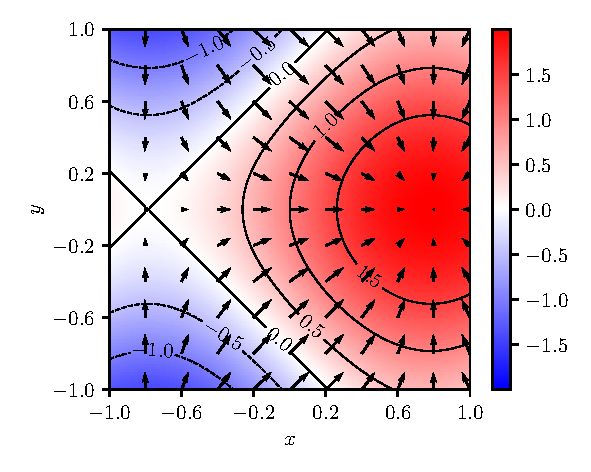
\includegraphics{./fig-gradient.pdf}
\caption{Skalárna funkcia $f(x, y) = \sin(2x) + \cos(2y)$ a~jej gradient 
$\nabla f(x, y)$ na~intervale $x, y \in [-1, 1]$.  Skalárna funkcia je 
znázornená hypsometricky a~izočiarami.  Gradient je zobrazený orientovanými 
šípkami, pričom šípka udáva smer a~veľkosť najväčšieho nárastu funkcie $f(x, 
y)$ v~danom bode.}
\label{fig:f_gradf}
\end{figure}






\chapter{Operátor gradient v~ortogonálnych súradnicových systémoch}
\label{app:gradient_in_orthogonal_systems}

V~tejto kapitole je vyjadrený operátor gradient v~ortogonálnych súradnicových 
systémoch.  \emph{Ortogonálny súradnicový systém} je taký súradnicový systém, 
ktorého súradnicové plochy sa pretínajú pod pravým uhlom.  Príkladom sú 
karteziánske súradnicové systémy~$(x, y, z)$ a~$(x^\mathrm{s}, y^\mathrm{s}, 
z^\mathrm{s})$ či~krivočiary systém súradníc~$(r, \varphi, \lambda)$ (pozri 
Obrázok~\ref{fig:cart_sph}).

V~Kapitole~\ref{app:gradient_in_spherical_coordinates} je odvodený operátor 
gradient~(\ref{eq:gradient_sph}) v~ortogonálnom krivočiarom sférickom 
súradnicovom systéme~$(r, \varphi, \lambda)$.  
V~Kapitole~\ref{app:gradient_in_orthogonal_coordinates} je uvedené všeobecné 
riešenie pre ľubovoľný ortogonálny súradnicový systém.



\section{Operátor gradient vo sférickom súradnicovom systéme}
\label{app:gradient_in_spherical_coordinates}

Nech je daná skalárna diferencovateľná funkcia $f$.  V~lokálnom karteziánskom 
súradnicovom systéme $x^{\mathrm{s}}$, $y^{\mathrm{s}}$, $z^{\mathrm{s}}$ 
s~jednotkovými vektormi $\vec e^\mathrm{s}_1$, $\vec e^\mathrm{s}_2$ a~$\vec 
e^\mathrm{s}_3$ (Obrázok~\ref{fig:cart_sph}) je gradient funkcie~$f$ daný 
vzťahom~(\ref{eq:gradient}),
%
\begin{equation}
\nabla f = \vec e^\mathrm{s}_1 \, \frac{\partial f}{\partial x^{\mathrm{s}}} 
+ \vec e^\mathrm{s}_2 \, \frac{\partial f}{\partial y^{\mathrm{s}}} + \vec 
e^\mathrm{s}_3 \, \frac{\partial f}{\partial z^{\mathrm{s}}}{.}
\end{equation}
%
Cieľom tejto kapitoly je vyjadriť parciálne derivácie $\partial f \slash 
\partial x^{\mathrm{s}}$, $\partial f \slash \partial y^{\mathrm{s}}$ 
a~$\partial f \slash \partial z^{\mathrm{s}}$ pomocou ortogonálnych 
\emph{krivočiarych} súradníc $\varphi$, $\lambda$, $r$ (pozri 
Obrázok~\ref{fig:cart_sph}).

Je zrejmé, že potrebujeme nájsť parciálne derivácie $\partial f \slash \partial 
\varphi$, $\partial f \slash \partial \lambda$ a~$\partial f \slash \partial 
r$.  Túto úlohu komplikuje závislosť karteziánskych súradníc $x$, $y$, $z$ od 
sférických súradníc $\varphi$, $\lambda$, $r$ (pozri 
rovnice~\ref{eq:sph2cart}).  Derivujeme preto zloženú funkciu troch premenných,
%
\begin{equation}
\label{eq:f_partials_rlatlon}
\begin{split}
\frac{\partial f}{\partial \varphi} &= \frac{\partial f}{\partial x} \, 
\frac{\partial x}{\partial \varphi} + \frac{\partial f}{\partial y} \, 
\frac{\partial y}{\partial \varphi} + \frac{\partial f}{\partial z} \, 
\frac{\partial z}{\partial \varphi}{,}\\[2ex]
%
\frac{\partial f}{\partial \lambda} &= \frac{\partial f}{\partial x} \, 
\frac{\partial x}{\partial \lambda} + \frac{\partial f}{\partial y} \, 
\frac{\partial y}{\partial \lambda} + \frac{\partial f}{\partial z} \, 
\frac{\partial z}{\partial \lambda}{,}\\[2ex]
%
\frac{\partial f}{\partial r} &= \frac{\partial f}{\partial x} \, 
\frac{\partial x}{\partial r} + \frac{\partial f}{\partial y} \, \frac{\partial 
y}{\partial r} + \frac{\partial f}{\partial z} \, \frac{\partial z}{\partial 
r}{.}
\end{split}
\end{equation}
%
Rovnicu~(\ref{eq:f_partials_rlatlon}) môžeme zapísať v~maticovom tvare
%
\begin{equation}
\label{eq:f_partials_rlatlon_2}
\begin{bmatrix}
\dfrac{\partial f}{\partial \varphi}\\[2ex]
\dfrac{\partial f}{\partial \lambda}\\[2ex]
\dfrac{\partial f}{\partial r}
\end{bmatrix}
%
=
%
\begin{bmatrix}
\dfrac{\partial x}{\partial \varphi} & \dfrac{\partial y}{\partial \varphi} 
& \dfrac{\partial z}{\partial \varphi}\\[2ex]
\dfrac{\partial x}{\partial \lambda} & \dfrac{\partial y}{\partial \lambda
} & \dfrac{\partial z}{\partial \lambda}\\[2ex]
\dfrac{\partial x}{\partial r} & \dfrac{\partial y}{\partial r} 
& \dfrac{\partial z}{\partial r}
\end{bmatrix}
%
\,
%
\begin{bmatrix}
\dfrac{\partial f}{\partial x}\\[2ex]
\dfrac{\partial f}{\partial y}\\[2ex]
\dfrac{\partial f}{\partial z}
\end{bmatrix}
%
{.}
\end{equation}

Zaveďme vektorovú funkciu~$\vec r$, ktorá bude popisovať začiatok lokálneho 
súradnicového systému $x^\mathrm{s}$, $y^\mathrm{s}$, $z^\mathrm{s}$ 
v~globálnom súradnicovom systéme $x$, $y$, $z$,
%
\begin{equation}
\label{eq:vector_r}
\vec r =
%
\begin{bmatrix}
x(\varphi, \lambda, r)\\
y(\varphi, \lambda, r)\\
z(\varphi, r)
\end{bmatrix}
%
{.}
\end{equation}
%
Vzťah~(\ref{eq:f_partials_rlatlon_2}) potom môžeme prepísať do tvaru
%
\begin{equation}
\label{eq:grad_cart2sph}
\begin{bmatrix}
\dfrac{\partial f}{\partial \varphi}\\[2ex]
\dfrac{\partial f}{\partial \lambda}\\[2ex]
\dfrac{\partial f}{\partial r}
\end{bmatrix}
%
=
%
\begin{bmatrix}
\left( \hat{\vec e}_1^\mathrm{s} \right)^\top\\
\left( \hat{\vec e}_2^\mathrm{s} \right)^\top\\
\left( \hat{\vec e}_3^\mathrm{s} \right)^\top
\end{bmatrix}
%
\,
%
\begin{bmatrix}
\dfrac{\partial f}{\partial x}\\[2ex]
\dfrac{\partial f}{\partial y}\\[2ex]
\dfrac{\partial f}{\partial z}
\end{bmatrix}
%
{,}
\end{equation}
%
kde symboly
%
\begin{equation}
\label{eq:er_elat_elon}
\begin{split}
\hat{\vec e}_1^\mathrm{s} &= \frac{\partial \vec r}{\partial \varphi} = 
%
\begin{bmatrix}
-r \, \sin\varphi \, \cos\lambda\\
-r \, \sin\varphi \, \sin\lambda\\
r \, \cos\varphi
\end{bmatrix}
%
{,}\\
%
\hat{\vec e}_2^\mathrm{s} &= \frac{\partial \vec r}{\partial \lambda} = 
%
\begin{bmatrix}
-r \, \cos\varphi \, \sin\lambda\\
r \, \cos\varphi \, \cos\lambda\\
0
\end{bmatrix}
%
{,}\\
%
\hat{\vec e}_3^\mathrm{s} &= \frac{\partial \vec r}{\partial r} = 
%
\begin{bmatrix}
\cos\varphi \, \cos\lambda\\
\cos\varphi \, \sin\lambda\\
\sin\varphi
\end{bmatrix}
%
\end{split}
\end{equation}
%
predstavujú vektory v~smere osí $x^{\mathrm{s}}$, $y^{\mathrm{s}}$ 
a $z^{\mathrm{s}}$ lokálneho karteziánskeho súradnicového systému.  Gradienty 
$\partial f \slash \partial x$, $\partial f \slash \partial y$, $\partial 
f \slash \partial z$ vyjadríme pomocou parciálnych derivácií $\partial f \slash 
\partial \varphi$, $\partial f \slash \partial \lambda$, $\partial f \slash 
\partial r$ vyriešením systému lineárnych rovníc~(\ref{eq:grad_cart2sph}) 
použitím niektorej z~metód lineárnej algebry.

Obzvlášť jednoduchá metóda riešenia systému rovníc~(\ref{eq:grad_cart2sph}) je 
nasledovná.  Normovaním vektorov~(\ref{eq:er_elat_elon}) získame jednotkové 
vektory v~smere súradnicových osí~$x^\mathrm{s}$, $y^\mathrm{s}$, 
$z^\mathrm{s}$,
%
\begin{equation}
\label{eq:er_elat_elon_unit}
\begin{aligned}
%
\vec e^\mathrm{s}_1 &= \frac{\hat{\vec e}_1^\mathrm{s}}{\| \hat{\vec 
e}_1^\mathrm{s} \|} = 
%
\begin{bmatrix}
-\sin\varphi \, \cos\lambda\\
-\sin\varphi \, \sin\lambda\\
\cos\varphi
\end{bmatrix}
%
{,} \quad &\| \hat{\vec e}_1^\mathrm{s} \| &= r{,}\\
%
\vec e^\mathrm{s}_2 &= \frac{\hat{\vec e}_2^\mathrm{s}}{\| \hat{\vec 
e}_2^\mathrm{s} \|} = 
%
\begin{bmatrix}
-\sin\lambda\\
\cos\lambda\\
0
\end{bmatrix}
%
{,}  \quad &\| \hat{\vec e}_2^\mathrm{s} \| &= r \, \cos\varphi{,}\\
%
\vec e^\mathrm{s}_3 &= \frac{\hat{\vec e}_3^\mathrm{s}}{\| \hat{\vec 
e}_3^\mathrm{s} \|} = 
%
\begin{bmatrix}
\cos\varphi \, \cos\lambda\\
\cos\varphi \, \sin\lambda\\
\sin\varphi
\end{bmatrix}
%
{,} \quad &\| \hat{\vec e}_3^\mathrm{s} \| &= 1{.}
%
\end{aligned}
\end{equation}
%
Lineárny systém rovníc~(\ref{eq:grad_cart2sph}) potom môžeme prepísať do tvaru
%
\begin{equation}
\label{eq:grad_cart2sph_2}
\begin{bmatrix}
\dfrac{\partial f}{\partial \varphi}\\[2ex]
\dfrac{\partial f}{\partial \lambda}\\[2ex]
\dfrac{\partial f}{\partial r}
\end{bmatrix}
%
=
%
\begin{bmatrix}
r \, \left( \vec e^\mathrm{s}_1\right)^\top\\
r \, \cos\varphi \, \left(\vec e^\mathrm{s}_2\right)^\top\\
\left(\vec e^\mathrm{s}_3\right)^\top
\end{bmatrix}
%
\,
%
\begin{bmatrix}
\dfrac{\partial f}{\partial x}\\[2ex]
\dfrac{\partial f}{\partial y}\\[2ex]
\dfrac{\partial f}{\partial z}
\end{bmatrix}
%
{.}
\end{equation}
%
O~vektoroch $\vec e^\mathrm{s}_1$, $\vec e^\mathrm{s}_2$, $\vec e^\mathrm{s}_3$ 
vieme, že sú ortogonálne (pozri rovnicu~\ref{eq:ei_orthogonality}) a~ich 
veľkosť je rovná~$1$, čo možno overiť vzťahmi~(\ref{eq:er_elat_elon_unit}).  
Inverzia matice systému lineárnych rovníc~(\ref{eq:grad_cart2sph_2}) je tak 
daná vzťahom \parencite{MichelLectures}
%
\begin{equation}
\begin{bmatrix}
r \, \left( \vec e^\mathrm{s}_1 \right)^\top\\[2ex]
r \, \cos\varphi \, \left( \vec e^\mathrm{s}_2 \right)^\top\\[2ex]
\left( \vec e^\mathrm{s}_3 \right)^\top
\end{bmatrix}^{-1}
%
=
%
\begin{bmatrix}
\dfrac{1}{r} \, \vec e^\mathrm{s}_1\\[2ex]
\dfrac{1}{r \, \cos\varphi} \, \vec e^\mathrm{s}_2\\[2ex]
\vec e^\mathrm{s}_3
\end{bmatrix}
{.}
\end{equation}
%
Riešenie rovnice~(\ref{eq:grad_cart2sph_2}) má teda tvar
%
\begin{equation}
\label{eq:grad_cart2sph_3}
\begin{bmatrix}
\dfrac{\partial f}{\partial x}\\[2ex]
\dfrac{\partial f}{\partial y}\\[2ex]
\dfrac{\partial f}{\partial z}
\end{bmatrix}
%
=
%
\begin{bmatrix}
\dfrac{1}{r} \, \vec e^\mathrm{s}_1\\[2ex]
\dfrac{1}{r \, \cos\varphi} \, \vec e^\mathrm{s}_2\\[2ex]
\vec e^\mathrm{s}_3
\end{bmatrix}
%
\,
%
\begin{bmatrix}
\dfrac{\partial f}{\partial \varphi}\\[2ex]
\dfrac{\partial f}{\partial \lambda}\\[2ex]
\dfrac{\partial f}{\partial r}
\end{bmatrix}
%
{.}
\end{equation}
%
Hľadané parciálne derivácie v~súradnicovom systéme~$x^\mathrm{s}$, 
$y^\mathrm{s}$, $z^\mathrm{s}$ sú tak dané vzťahmi
%
\begin{equation}
\label{eq:lnof_diff_oeprators}
\begin{split}
\frac{\partial f}{\partial x^\mathrm{s}} &= \frac{1}{r} \, \frac{\partial 
f}{\partial \varphi}{,}\\
%
\frac{\partial f}{\partial y^\mathrm{s}} &= \frac{1}{r \, \cos\varphi} \, 
\frac{\partial f}{\partial \lambda}{,}\\
%
\frac{\partial f}{\partial z^\mathrm{s}} &= \frac{\partial f}{\partial r}{.}
\end{split}
\end{equation}
%
Keďže funkcia~$f$ je ľubovoľná skalárna diferencovateľná funkcia (pozri 
začiatok tejto kapitoly), vzťah~(\ref{eq:grad_cart2sph_3}) dokazuje 
rovnicu~(\ref{eq:gradient_sph}).




\section{Operátor gradient v~ortogonálnom súradnicovom systéme}
\label{app:gradient_in_orthogonal_coordinates}

Odvodenie z~predošlej kapitoly možno zovšeobecniť na ľubovoľný ortogonálny 
súradnicový systém.  Nech je daný ortogonálny súradnicový systém $\xi_1$, 
$\xi_2$, $\xi_3$ a~diferencovateľná funkcia~$f$.  Gradient funkcie~$f$ je 
v~tomto súradnicovom systéme daný vzťahom 
\parencite{Arfken2005,SansoGeoidDetermination}
%
\begin{equation}
\label{eq:grad_orthogonal_system}
\nabla f = \sum_{i = 1}^3 \frac{\hat{\vec e}_i}{\| \hat{\vec e}_i \|^2} \, 
\frac{\partial f}{\partial \xi_i} = \sum_{i = 1}^3 \frac{1}{\| \hat{\vec e}_i 
\|} \, \vec e_i \, \frac{\partial f}{\partial \xi_i}{,}
\end{equation}
%
kde
%
\begin{equation}
\label{eq:xi1xi2xi3_vectors}
\hat{\vec e}_i = \frac{\partial \vec r(\boldsymbol \xi)}{\partial \xi_i}
\end{equation}
%
je vektor v~smere súradnicovej osi~$\xi_i$,
%
\begin{equation}
\label{eq:xi1xi2xi3_unit_vectors}
\vec e_i = \frac{\hat{\vec e}_i}{\| \hat{\vec e}_i \|}
\end{equation}
%
je jednotkový vektor v~smere súradnicovej osi~$\xi_i$~a
%
\begin{equation}
\boldsymbol \xi =
%
\begin{bmatrix}
\xi_1\\
\xi_2\\
\xi_3
\end{bmatrix}
%
{.}
%
\end{equation}






\chapter{Laplaceov operátor v~ortogonálnych súradnicových systémoch}
\label{app:laplace_in_spherical_coordinates}

V~Kapitole~\ref{app:laplace_in_spherical_system} je odvodený Laplaceov operátor 
vo sférickom súradnicovom systéme (rovnica~\ref{eq:vg_laplace_sph}).  
V~Kapitole~\ref{app:laplace_in_orthogonal_coordinates} je odvodený všeobecný 
tvar Laplaceovho operátora v~ortogonálnom súradnicovom systéme.



\section{Laplaceov operátor vo sférickom súradnicovom systéme}
\label{app:laplace_in_spherical_system}

Laplaceov operátor vo sférickych súradniciach vyjadríme pomocou operátora 
gradient~(\ref{eq:gradient_sph}), ktorý dosadíme do 
rovnice~(\ref{eq:laplace_grad_grad_notation}) a~aplikujeme 
v~zmysle~(\ref{eq:laplace_xyz}),
%
\begin{align}
\label{eq:grad_grad_sph}
\nabla^2 &= \nabla \cdot \nabla\nonumber\\
%
&= \left( \vec e_1^\mathrm{s} \, \frac{1}{r} \, \frac{\partial}{\partial 
\varphi} + \vec e_2^\mathrm{s} \, \frac{1}{r \, \cos\varphi} \, 
\frac{\partial}{\partial \lambda} + \vec e_3^\mathrm{s} 
\frac{\partial}{\partial r} \right) \cdot \left( \vec e_1^\mathrm{s} \, 
\frac{1}{r} \, \frac{\partial}{\partial \varphi} + \vec e_2^\mathrm{s} \, 
\frac{1}{r \, \cos\varphi} \, \frac{\partial}{\partial \lambda} + \vec 
e_3^\mathrm{s} \frac{\partial}{\partial r} \right)\nonumber\displaybreak[2]\\
%
&= \frac{1}{r^2} \, \underbrace{\vec e^\mathrm{s}_1 \cdot \frac{\partial \vec 
e^\mathrm{s}_1}{\partial \varphi}}_{\vec e_1^\mathrm{s} \cdot (- \vec 
e_3^\mathrm{s}) = 0} \, \frac{\partial}{\partial \varphi} + \frac{1}{r^2} \, 
\underbrace{\vec e^\mathrm{s}_1 \cdot \vec e^\mathrm{s}_1}_{1} \, 
\frac{\partial^2}{\partial \varphi^2} + \frac{1}{r^2 \, \cos\varphi} \, 
\underbrace{\vec e_1^\mathrm{s} \cdot \frac{\partial \vec 
e_2^\mathrm{s}}{\partial \varphi}}_{\vec e_1^\mathrm{s} \cdot \vec 0 = 0} \, 
\frac{1}{\partial \lambda}\nonumber\displaybreak[2]\\
%
&\phantom{={}}+ \frac{1}{r} \, \underbrace{\vec e_1^\mathrm{s} \cdot \vec 
e_2^\mathrm{s}}_{0} \, \frac{1}{\partial \varphi} \left( \frac{1}{r \, 
\cos\varphi} \right) \, \frac{\partial}{\partial \lambda} + \frac{1}{r^2 \, 
\cos\varphi} \, \underbrace{\vec e_1^\mathrm{s} \cdot \vec e_2^\mathrm{s}}_{0} 
\, \frac{\partial^2}{\partial \varphi \, \partial \lambda} + \frac{1}{r} \, 
\underbrace{\vec e_1^\mathrm{s} \cdot \frac{\partial \vec 
e_3^\mathrm{s}}{\partial \varphi}}_{\vec e_1^\mathrm{s} \cdot \vec 
e_1^\mathrm{s} = 1} \, \frac{\partial}{\partial r}\nonumber\displaybreak[2]\\
%
&\phantom{={}}+ \frac{1}{r} \, \underbrace{\vec e_1^\mathrm{s} \cdot \vec 
e_3^\mathrm{s}}_{0} \, \frac{\partial^2}{\partial \varphi \, \partial r} 
+ \frac{1}{r^2 \, \cos\varphi} \, \underbrace{\vec e_2^\mathrm{s} \cdot 
\frac{\partial \vec e_1^\mathrm{s}}{\partial \lambda}}_{\vec e_2^\mathrm{s} 
\cdot (-\sin\varphi \, \vec e_2^\mathrm{s}) = -\sin\varphi} \, 
\frac{\partial}{\partial \varphi} + \frac{1}{r^2 \, \cos\varphi} \, 
\underbrace{\vec e_2^\mathrm{s} \cdot \vec e_1^\mathrm{s}}_{0} \, 
\frac{\partial^2}{\partial \varphi \, \partial \lambda}\displaybreak[2]\\
%
&\phantom{={}}+ \frac{1}{r^2 \, \cos^2\varphi} \, \underbrace{\vec 
e_2^\mathrm{s} \cdot \frac{\partial \vec e_2^\mathrm{s}}{\partial \lambda}}_{0} 
\, \frac{\partial}{\partial\lambda} + \frac{1}{r^2 \, \cos^2\varphi} \, 
\underbrace{\vec e_2^\mathrm{s} \cdot \vec e_2^\mathrm{s}}_{1} \, 
\frac{\partial^2}{\partial\lambda^2} + \frac{1}{r \, \cos\varphi} \, 
\underbrace{\vec e_2^\mathrm{s} \cdot \frac{\partial \vec 
e_3^\mathrm{s}}{\partial \lambda}}_{\vec e_2^\mathrm{s} \cdot (\cos\varphi \, 
\vec e_2^\mathrm{s}) = \cos\varphi} \, \frac{\partial}{\partial 
r}\nonumber\displaybreak[2]\\
%
&\phantom{={}}+ \frac{1}{r \, \cos\varphi} \, \underbrace{\vec e_2^\mathrm{s} 
\cdot \vec e_3^\mathrm{s}}_{0} \, \frac{\partial^2}{\partial \lambda \, 
\partial r} + \frac{1}{r} \, \underbrace{\vec e_3^\mathrm{s} \cdot 
\frac{\partial \vec e_1^\mathrm{s}}{\partial r}}_{\vec e_3^\mathrm{s} \cdot 
\vec 0 = 0} \, \frac{\partial}{\partial \varphi} + \underbrace{\vec 
e_3^\mathrm{s} \cdot \vec e_1^\mathrm{s}}_{0} \, \frac{\partial}{\partial r} 
\left( \frac{1}{r} \right) \, \frac{\partial}{\partial \varphi} 
+ \underbrace{\vec e_3^\mathrm{s} \cdot \vec e_1^\mathrm{s}}_{0} \, \frac{1}{r} 
\, \frac{\partial^2}{\partial r \, \partial \varphi}\nonumber\displaybreak[2]\\
%
&\phantom{={}}+\frac{1}{r \, \cos\varphi} \, \underbrace{\vec e_3^\mathrm{s} 
\cdot \frac{\partial \vec e_2^\mathrm{s}}{\partial r}}_{\vec e_3^\mathrm{s} 
\cdot \vec 0 = 0} \, \frac{\partial}{\partial \lambda} + \underbrace{\vec 
e_3^\mathrm{s} \cdot \vec e_2^\mathrm{s}}_{0} \, \frac{\partial}{\partial r} \, 
\left( \frac{1}{r \, \cos\varphi} \right) \, \frac{\partial^2}{\partial r \, 
\partial \lambda} + \underbrace{\vec e_3^\mathrm{s} \cdot \frac{\partial \vec 
e_3^\mathrm{s}}{\partial r}}_{\vec e_3^\mathrm{s} \cdot \vec 0 = 0} \, 
\frac{\partial}{\partial r} + \underbrace{\vec e_3^\mathrm{s} \cdot \vec 
e_3^\mathrm{s}}_{1} \, \frac{\partial^2}{\partial r^2}{.}\nonumber
\end{align}
%
Jednotkové vektory $\vec e_1^\mathrm{s}$, $\vec e_2^\mathrm{s}$ a~$\vec 
e_3^\mathrm{s}$ vystupujúce v~predošlej rovnici sú dané 
vzťahmi~(\ref{eq:er_elat_elon_unit}).  Ich derivácie podľa sférických súradníc 
majú nasledovný tvar,
%
\begin{equation}
\label{eq:er_elat_elon_unit_derivatives}
\begin{split}
\frac{\partial \vec e_1^\mathrm{s}}{\partial \varphi} &=
%
\begin{bmatrix}
-\cos\varphi \, \cos\lambda\\
-\cos\varphi \, \sin\lambda\\
-\sin\varphi\\
\end{bmatrix}
%
= -\vec e_3^\mathrm{s}
%
{,}\\
%
\frac{\partial \vec e_1^\mathrm{s}}{\partial \lambda} &=
%
\begin{bmatrix}
 \sin\varphi \, \sin\lambda\\
-\sin\varphi \, \cos\lambda\\
0\\
\end{bmatrix}
%
= -\sin\varphi \, \vec e_2^\mathrm{s}
%
{,}\\
%
\frac{\partial \vec e_1^\mathrm{s}}{\partial r} &= \vec 0{,}\\
%
\frac{\partial \vec e_2^\mathrm{s}}{\partial \varphi} &= \vec 0{,}\\
%
\frac{\partial \vec e_2^\mathrm{s}}{\partial \lambda} &=
%
\begin{bmatrix}
-\cos\lambda\\
-\sin\lambda\\
0\\
\end{bmatrix}
%
{,}\\
%
\frac{\partial \vec e_2^\mathrm{s}}{\partial r} &= \vec 0{,}\\
%
\frac{\partial \vec e_3^\mathrm{s}}{\partial \varphi} &=
%
\begin{bmatrix}
-\sin\varphi \, \cos\lambda\\
-\sin\varphi \, \sin\lambda\\
\cos\varphi\\
\end{bmatrix}
%
= \vec e_1^\mathrm{s}
%
{,}\\
%
\frac{\partial \vec e_3^\mathrm{s}}{\partial \lambda} &=
%
\begin{bmatrix}
-\cos\varphi \, \sin\lambda\\
 \cos\varphi \, \cos\lambda\\
0\\
\end{bmatrix}
%
= \cos\varphi \, \vec e_2^\mathrm{s}
%
{,}\\
%
\frac{\partial \vec e_3^\mathrm{s}}{\partial r} &= \vec 0{.}
\end{split}
\end{equation}
%
Kombináciou rovníc~(\ref{eq:grad_grad_sph}) 
a~(\ref{eq:er_elat_elon_unit_derivatives}) získame Laplaceov operátor vo 
sférických súradniciach,
%
\begin{equation}
\label{eq:laplace_sph}
\nabla^2 = \frac{1}{r^2} \frac{\partial}{\partial r} \left( r^2
\frac{\partial}{\partial r} \right) + \frac{1}{r^2 \, \cos\varphi}
\frac{\partial}{\partial \varphi} \left( \cos\varphi \frac{\partial}{\partial 
\varphi} \right) + \frac{1}{r^2 \,
\cos^2\varphi}\frac{\partial^2}{\partial \lambda^2}{.}
\end{equation}

\subsubsection{Poznámka o~nesprávnej interpretácii vektorového zápisu operátora 
gradient}

Vráťme sa k~diskusii o~Laplaceovom operátore 
z~Kapitoly~\ref{sec:laplace_equation_cart}.  V~predchádzajúcej časti sme 
ukázali, že správna aplikácia operátora gradient~(\ref{eq:gradient_sph}) 
v~rovnici~(\ref{eq:laplace_grad_grad_notation}) vedie k~Laplaceovmu operátoru 
vo sférických súradniciach~(\ref{eq:laplace_sph}).  Nesprávnym použitím 
operátora~(\ref{eq:gradient_sph}), teda vynásobením zodpovedajúcich si prvkov 
vektora na pravej strane rovnice~(\ref{eq:gradient_sph}) a~následným sčítaním 
získaných súčinov, dostaneme operátor
%
\begin{equation}
\frac{1}{r^2} \frac{\partial^2}{\partial \varphi^2} + \frac{1}{r^2 \, 
\cos^2\varphi} \frac{\partial^2}{\partial \lambda^2} 
+ \frac{\partial^2}{\partial r^2}{,}
\end{equation}
%
čo však nie je Laplaceov operátor vo sférických súradniciach.




\section{Laplaceov operátor v~ortogonálnom súradnicovom systéme}
\label{app:laplace_in_orthogonal_coordinates}

Odvodenie z~predchádzajúcej kapitoly možno zovšeobecniť na ľubovoľný 
ortogonálny súradnicový systém $\xi_1$, $\xi_2$, $\xi_3$.  Táto kapitola je 
spracovaná podľa~\textcite{SansoGeoidDetermination}.

Všeobecný tvar Laplaceovho operátora získame pomocou 
rovníc~(\ref{eq:laplace_grad_grad_notation}) 
a~(\ref{eq:grad_orthogonal_system}),
%
\begin{equation}
\label{eq:laplace_orthogonal_system_1}
\begin{split}
\nabla^2 &= \nabla \cdot \nabla = \left( \sum_{i = 1}^3 \frac{\hat{\vec 
e}_i}{\| \hat{\vec e}_i \|^2} \, \frac{\partial}{\partial \xi_i}\right) \cdot 
\left( \sum_{j = 1}^3 \frac{\hat{\vec e}_j}{\| \hat{\vec e}_j \|^2} \, 
\frac{\partial}{\partial \xi_j}
\right)\\
%
&= \sum_{i = 1}^{3} \sum_{j = 1}^3 \frac{1}{\| \hat{\vec e}_i \|^2 \, \| 
\hat{\vec e}_j \|^2} \, \hat{\vec e}_i \cdot \frac{\partial \hat{\vec 
e}_j}{\partial \xi_i} \, \frac{\partial}{\partial \xi_j}
- 2\, \sum_{i = 1}^{3} \sum_{j = 1}^3 \frac{\hat{\vec e}_i \cdot \hat{\vec 
e}_j}{\| \hat{\vec e}_i \|^2 \, \|\hat{\vec e}_j \|^3} \, \frac{\partial \| 
\hat{\vec e}_j \|}{\partial \xi_i} \, \frac{\partial}{\partial \xi_j}\\
%
&\phantom{={}}+ \sum_{i = 1}^{3} \sum_{j = 1}^3 \frac{\hat{\vec e}_i \cdot 
\hat{\vec e}_j}{\| \hat{\vec e}_i \|^2 \, \| \hat{\vec e}_j \|^2} \, 
\frac{\partial^2}{\partial \xi_i \, \partial \xi_j}{.}
\end{split}
%
\end{equation}

Keďže súradnicový systém $\xi_1$, $\xi_2$, $\xi_3$ je podľa predpokladu 
ortogonálny, vektory~$\hat{\vec e}_i$, $i = 1, 2, 3$, musia byť taktiež 
ortogonálne (pozri vzťahy~\ref{eq:ei_orthogonality}, \ref{eq:ei_unit_length}, 
\ref{eq:xi1xi2xi3_vectors} a~\ref{eq:xi1xi2xi3_unit_vectors}),
%
\begin{equation}
\label{eq:hat_e_ij_orthogonality}
\hat{\vec e}_i \cdot \hat{\vec e}_j =
%
\begin{cases}
\left( \| \hat{\vec e}_i \| \, \vec e_i \right) \cdot \left( \| \hat{\vec e}_i 
\| \, \vec e_i \right) = \| \hat{\vec e}_i \|^2{,} \quad &\textrm{ak} \quad 
i = j{,}\\
0{,} \quad &\textrm{ak} \quad i \neq j{.}
\end{cases}
\end{equation}
%
Použitím vzťahov
%
\begin{equation}
\label{eq:partials_hat_e}
\frac{\partial \hat{\vec e}_i}{\partial \xi_j} = \frac{\partial}{\partial 
\xi_j} \, \frac{\partial \vec r(\boldsymbol \xi)}{\partial \xi_i} 
= \frac{\partial}{\partial \xi_i} \, \frac{\partial \vec r(\boldsymbol 
\xi)}{\partial \xi_j} = \frac{\partial \hat{\vec e}_j}{\partial \xi_i}
\end{equation}
%
a~(\ref{eq:hat_e_ij_orthogonality}) prejde 
rovnica~(\ref{eq:laplace_orthogonal_system_1}) do tvaru
%
\begin{equation}
\label{eq:laplace_orthogonal_system_2}
\begin{split}
\nabla^2 &= \sum_{i = 1}^{3} \sum_{j = 1}^3 \frac{1}{\| \hat{\vec e}_i \|^2 \, 
\| \hat{\vec e}_j \|^2} \, \hat{\vec e}_i \cdot \frac{\partial \hat{\vec 
e}_i}{\partial \xi_j} \, \frac{\partial}{\partial \xi_j}
- 2\, \sum_{j = 1}^{3} \frac{1}{\|\hat{\vec e}_j \|^3} \, \frac{\partial \| 
\hat{\vec e}_j \|}{\partial \xi_j} \, \frac{\partial}{\partial \xi_j}\\
%
&\phantom{={}}+ \sum_{j = 1}^3 \frac{1}{\| \hat{\vec e}_j \|^2} \, 
\frac{\partial^2}{\partial \xi_j^2}{.}
\end{split}
%
\end{equation}

Ďalej samostatne upravíme najprv prvé dva členy 
rovnice~(\ref{eq:laplace_orthogonal_system_2}) a~následne jej tretí člen.  Na 
záver použijeme výsledky oboch úprav, čím získame výsledný tvar Laplaceovho 
operátora v~ľubovoľnom ortogonálnom súradnicovom systéme~$\xi_1$, $\xi_2$, 
$\xi_3$.

Nech $j = 1$.  Prvé dva členy rovnice~(\ref{eq:laplace_orthogonal_system_2}) 
potom môžeme upraviť nasledovne,
%
\begin{equation}
\label{eq:laplace_orthogonal_system_two_terms}
\begin{split}
&\sum_{i = 1}^{3} \frac{1}{\| \hat{\vec e}_i \|^2 \, \| \hat{\vec e}_1 \|^2} \, 
\hat{\vec e}_i \cdot \frac{\partial \hat{\vec e}_i}{\partial \xi_1} \, 
\frac{\partial}{\partial \xi_1}
- 2\, \frac{1}{\|\hat{\vec e}_1 \|^3} \, \frac{\partial \| \hat{\vec e}_1 
\|}{\partial \xi_1} \, \frac{\partial}{\partial \xi_1}\\
%
&= \sum_{i = 1}^{3} \frac{1}{\| \hat{\vec e}_i \|^2 \, \| \hat{\vec e}_1 \|^2} 
\, \| \hat{\vec e}_i \| \, \frac{\partial \| \hat{\vec e}_i \|}{\partial \xi_1} 
\, \frac{\partial}{\partial \xi_1}
- 2\, \frac{1}{\|\hat{\vec e}_1 \|^3} \, \frac{\partial \| \hat{\vec e}_1 
\|}{\partial \xi_1} \, \frac{\partial}{\partial \xi_1}\\
%
&= -\frac{1}{\| \hat{\vec e}_1 \|^3} \, \frac{\partial \| \hat{\vec e}_1 
\|}{\partial \xi_1} \, \frac{\partial}{\partial \xi_1} + \frac{1}{\| \hat{\vec 
e}_1 \|^2 \, \| \hat{\vec e}_2 \|} \, \frac{\partial \| \hat{\vec e}_2 
\|}{\partial \xi_1} \, \frac{\partial}{\partial \xi_1} + \frac{1}{\| \hat{\vec 
e}_1 \|^2 \, \| \hat{\vec e}_3 \|} \, \frac{\partial \| \hat{\vec e}_3 
\|}{\partial \xi_1} \, \frac{\partial}{\partial \xi_1}\\
%
&= \frac{1}{\| \hat{\vec e}_1 \| \, \| \hat{\vec e}_2 \| \, \| \hat{\vec e}_3 
\|} \, \frac{\partial}{\partial \xi_1} \, \left( \frac{\| \hat{\vec e}_2 \| \, 
\| \hat{\vec e}_3 \|}{\| \hat{\vec e}_1 \|} \right) \, \frac{\partial}{\partial 
\xi_1}{.}
\end{split}
\end{equation}
%
V rovnici~(\ref{eq:laplace_orthogonal_system_two_terms}) sme využili vzťah
%
\begin{equation}
\hat{\vec e}_i \cdot \frac{\partial \hat{\vec e}_i}{\partial \xi_j} 
= \frac{1}{2} \, \frac{\partial}{\partial \xi_j} \, \left( \hat{\vec e}_i \cdot 
\hat{\vec e}_i \right) = \frac{1}{2} \, \frac{\partial \| \hat{\vec e}_i 
\|^2}{\partial \xi_j} = \| \hat{\vec e}_i \| \, \frac{\partial \| \hat{\vec 
e}_i \|}{\partial \xi_j}{.}
\end{equation}
%
Použitím substitúcie
%
\begin{equation}
\label{eq:e_laplace}
E = \| \hat{\vec e}_1  \| \, \| \hat{\vec e}_2  \| \, \| \hat{\vec e}_3  \|
\end{equation}
%
a spôsobom podobným odvodeniu 
vzťahu~(\ref{eq:laplace_orthogonal_system_two_terms}) možno upraviť prvé dva 
členy rovnice~(\ref{eq:laplace_orthogonal_system_2}) pre všetky $j = 1, 2, 3$ 
do konečného tvaru
%
\begin{equation}
\label{eq:laplace_orthogonal_system_two_terms_final}
\frac{1}{E} \, \sum_{j = 1}^3 \left( \frac{\partial}{\partial \xi_j} \, 
\frac{E}{\| \hat{\vec e}_j \|^2}\right) \, \frac{\partial}{\partial \xi_j}{.}
\end{equation}

Tretí člen rovnice~(\ref{eq:laplace_orthogonal_system_2}) upravíme pomocou 
vzťahu~(\ref{eq:e_laplace}),
%
\begin{equation}
\label{eq:laplace_orthogonal_system_third_term}
\sum_{j = 1}^3 \frac{1}{\| \hat{\vec e}_j \|} \, \frac{\partial^2}{\partial 
\xi_j^2} = \frac{1}{E} \, \sum_{j = 1}^3 \frac{E}{\| \hat{\vec e}_j \|^2} \, 
\frac{\partial^2}{\partial \xi_j^2}{.}
\end{equation}

Kombináciou~(\ref{eq:laplace_orthogonal_system_two_terms_final}) 
a~(\ref{eq:laplace_orthogonal_system_third_term}) získame výsledný tvar 
Laplaceovho operátora v~ortogonálnom súradnicovom systéme,
%
\begin{equation}
\label{eq:laplace_orthogonal_system_final}
\begin{split}
\nabla^2 &= \frac{1}{E} \, \sum_{j = 1}^3 \left( \frac{\partial}{\partial 
\xi_j} \, \frac{E}{\| \hat{\vec e}_j \|^2}\right) \, \frac{\partial}{\partial 
\xi_j} + \frac{1}{E} \, \sum_{j = 1}^3 \, \frac{E}{\| \hat{\vec e}_j \|^2} \, 
\frac{\partial^2}{\partial \xi_j^2}\\
%
&= \frac{1}{E} \, \sum_{j = 1}^3 \frac{\partial}{\partial \xi_j} \left( 
\frac{E}{\| \hat{\vec e}_j  \|^2} \, \frac{\partial}{\partial \xi_j} \right){.}
\end{split}
\end{equation}
%
Dosadením substitúcie~(\ref{eq:e_laplace}) 
do~(\ref{eq:laplace_orthogonal_system_final}) dostaneme tvar Laplaceovho 
operátora, s~ktorým sa možno často stretnúť v~literatúre 
\parencite[napríklad][]{MoritzPhysicalGeodesy},
%
\begin{equation}
\label{eq:laplace_orthogonal_system_final_2}
\begin{split}
\nabla^2 &= \frac{1}{\| \hat{\vec e}_1 \| \, \| \hat{\vec e}_2 \| \, \| 
\hat{\vec e}_3 \|} \, \left[ \frac{\partial}{\partial \xi_1} \left( \frac{\| 
\hat{\vec e}_2 \| \, \| \hat{\vec e}_3 \|}{\| \hat{\vec e}_1 \|} \, 
\frac{\partial}{\partial \xi_1} \right) + \frac{\partial}{\partial \xi_2} 
\left( \frac{\| \hat{\vec e}_1 \| \, \| \hat{\vec e}_3 \|}{\| \hat{\vec e}_2 
\|} \, \frac{\partial}{\partial \xi_2} \right) \right.\\
%
&\phantom{={}}\left. + \frac{\partial}{\partial \xi_3} \left( \frac{\| 
\hat{\vec e}_1 \| \, \| \hat{\vec e}_2 \|}{\| \hat{\vec e}_3 \|} \, 
\frac{\partial}{\partial \xi_3} \right)\right]{.}
\end{split}
\end{equation}

Z~rovnice~(\ref{eq:laplace_orthogonal_system_final_2}) vidíme, že na získanie 
Laplaceovho operátora v~ortogonálnom súradnicovom systéme postačuje vypočítať 
veľkosti vektorov $\hat{\vec e}_i$ a~dosadiť ich do tohto vzťahu.




\chapter{Výpočet a~zobrazenie Legendreových polynómov}
\label{app:lp}

Zdrojový kód~\ref{src:lp} vypočíta a~graficky znázorní Legendreove polynómy 
$P_n(t) = P_n(\sin\varphi)$ stupňov $n = 0, 1, \dots, n_{\max}$ pre $\varphi 
\in [-\frac{\pi}{2}, \frac{\pi}{2}]$.  Polynómy sú pre názornosť počítané 
Bonnetovým rekurentným vzťahom~(\ref{eq:pn_bonnet}), ktorý je vhodný na 
praktickú numerickú implementáciu.  Funkciou 
\texttt{scipy.special.eval\_legendre} z~modulu \texttt{scipy} je možné 
vypočítať Legendreove funkcie bez nutnosti programovania rekurentných vzťahov.

\lstinputlisting[caption=Výpočet a~zobrazenie Legendreových polynómov
v~programovacom jazyku Python, language=mypython, label=src:lp,
captionpos=t]{../python/legendre-polynomials.py}






\chapter{Výpočet a~zobrazenie sférických harmonických funkcií}
\label{app:sh}

Zdrojový kód~\ref{src:ynk} vypočíta a~zobrazí nenormovanú plošnú sférickú
harmonickú funkciu stupňa $n$ a~rádu $k = -n, \dots, n$
(rovnica~\ref{eq:ynk_no_norm}).  Legendreove funkcie sú pre jednoduchosť
počítané funkciou \texttt{lpmv} z~Python modulu \texttt{scipy}.  Táto funkcia
počíta Legendreove funkcie $P_n^{|k|}(\sin\varphi)$, v~ktorých je
použitý Condonov--Shortlyho fázový faktor (pozri 
Kapitolu~\ref{sec:legendre_functions_cs_factor}).  Vo fyzikálnej geodézii sa 
tento faktor väčšinou nepoužíva, preto je vo výpočte odstránený.


\lstinputlisting[caption=Výpočet a~zobrazenie nenormovaných sférických
harmonických funkcií v~programovacom jazyku Python, label=src:ynk,
language=mypython, captionpos=t]{../python/spherical-harmonics.py}






\chapter{Ukážka modelu gravitačného poľa Zeme}
\label{app:gfc_file}

Táto príloha obsahuje ukážku modelu EIGEN-6C4 vo forme \texttt{gfc} súboru.  
Niektoré odkazy na literatúru zo state \texttt{References} a~mnohé sférické 
harmonické koeficienty sú pre stručnosť vynechané.  Preskočené časti sú 
označené značkou \texttt{[...]}.  Pôvodný súbor je dostupný zo stránky služby 
ICGEM (pozri odkaz na stránku v~hlavnej časti práce 
v~Kapitole~\ref{sec:sh_applications_gravity_field}).  Sférický harmonický 
stupeň~$n$ a~rád~$m$ sú v~modeli označené písmenami~\texttt{L} a~\texttt{M}.  
Stĺpce s~označením~\texttt{sigma C} a~\texttt{sigma S} obsahujú formálne 
stredné chyby príslušných sférických harmonických koeficientov.

\vspace{10ex}

\noindent\texttt{The Gravity Field Model EIGEN-6C4\\
\noindent -----------------------------------------------------------------\\
\\
\noindent EIGEN-6C4 is a static global combined gravity field model up to 
degree and order 2190.  It has been elaborated jointly  by GFZ Potsdam and GRGS 
Toulouse and contains the following  satellite and ground data:
\\
\\
\noindent - LAGEOS (deg. 2 - 30): 1985 - 2010
\\
\\
\noindent - GRACE RL03 GRGS (deg. 2 - 130): ten years 2003 - 2012
\\
\\
\noindent - GOCE-SGG data, processed by the direct approach (Pail et 
al. 2011,\\
\phantom{- }Bruinsma et al. 2014, to deg. 235) incl. the gravity gradient\\
\phantom{- }components Txx, Tyy, Tzz and Txz out of the following time spans:\\
\phantom{- }837 days out of the nominal mission time span 20091101 - 20120801\\
\phantom{- }422 days out of the lower orbit phase between 20120901 - 20130524\\
\phantom{- }The GOCE polar gaps were stabilized by the Spherical Cap 
Regularization\\
\phantom{- }(Metzler and Pail 2005) using the combined gravity field model\\
\phantom{- }EIGEN-6C3stat\\
\\
\noindent - Terrestrial data (max degree 370):\\
\phantom{- }DTU12 ocean geoid data (Anderson et al. 2009) and an EGM2008 geoid 
\phantom{- }height grid for the continents
\\
\\
\noindent The combination of these different satellite and surface data sets 
has been done by a band-limited combination of normal equations (to max degree 
370), which are generated from observation equations for the spherical harmonic 
coefficients. A brief description of the applied techniques for the generation 
of such a combined gravity field model is given in Shako et al. 2014. The 
resulted solution to degree/order 370 has been extended to degree/order 2190 by 
a block diagonal solution using the DTU10 global gravity anomaly data grid.
\\
\\
\noindent References:\\
\noindent ----------------------
\\
\\
\noindent Andersen O. B. P. Knudsen and P. Berry. (2009): DNSC08 mean sea 
surface and mean dynamic topography models, Journal of Geophys Research, 
Vol. 114, c11001 12 pp., 2009, doi:10.1029/2008JC005179
\\
\\
\noindent [...]
\\
\\
\noindent begin\_of\_head =====================================\\
\noindent product\_type\phantom{***************}gravity\_field\\
\noindent modelname\phantom{******************}EIGEN-6C4\\
\noindent earth\_gravity\_constant\phantom{*****}0.3986004415E+15\\
\noindent radius\phantom{*********************}0.6378136460E+07\\
\noindent max\_degree\phantom{*****************}2190\\
\noindent errors\phantom{*********************}formal\\
\noindent norm\phantom{***********************}fully\_normalized\\
\noindent tide\_system\phantom{****************}tide\_free\\
\\
\noindent key    L    M \phantom{-}C \phantom{-------------------------------}S 
\phantom{----------------------------------}sigma C   \phantom{------}sigma S\\
\noindent end\_of\_head 
=======================================================\\
\noindent gfc    0    0  \phantom{-}1.00000000000e+00 0.000000000000e+00 0.0000e+00 0.0000e+00\\
\noindent gfc    1    0  \phantom{-}0.00000000000e+00 0.000000000000e+00 0.0000e+00 0.0000e+00\\
\noindent gfc    2    0 -4.84165217061e-04 0.000000000000e+00 1.1081e-13 0.0000e+00\\
\noindent gfc    3    0  \phantom{-}9.57173592933e-07 0.000000000000e+00 6.5264e-14 0.0000e+00\\
\\
\noindent [...]
\\
\\
\noindent gfc    1    1 \phantom{-}0.00000000000e+00 0.00000000000e+00 0.0000e+00 0.0000e+00\\
\noindent gfc    2    1 -3.38846075704e-10  1.46306108906e-09 3.2499e-13 3.2870e-13\\
\noindent gfc    3    1 \phantom{-}2.03045608898e-06  2.48236210655e-07 
8.5500e-14 8.5499e-14\\
\\
\noindent [...]
\\
\\
\noindent \mbox{gfc 2190 2190 -0.488605221310D-13 -0.515141038060D-13 0.1601D-12 0.1601D-12}
}






\chapter{Výpočet a~zobrazenie sférického harmonického rozvoja zemskej
topografie}
\chaptermark{Výpočet a~zobrazenie sférického harmonického rozvoja}
\label{app:shs_topography}

Zdrojovým kódom~\ref{src:h_shs} je možné vypočítať a~zobraziť sférický 
harmonický rozvoj topografie Zeme.  Sférické harmonické koeficienty 
$\bar{h}_{nk}$ (pozri rovnicu~\ref{eq:h_shs}) sú prevzaté z~modelu DTM2006.0 
\parencite{DTM2006}.  Výpočet používa program GrafLab \parencite{GrafLab}, 
ktorý je voľne dostupný na adrese 
\url{https://github.com/blazej-bucha/graflab}.  Návody na prácu v~programe 
GrafLab je možné nájsť na adrese 
\url{https://github.com/blazej-bucha/graflab-cookbook}.

\lstinputlisting[caption=Sférický harmonický rozvoj zemskej topografie
v~programovacom jazyku MATLAB, label=src:h_shs, language=matlab,
captionpos=t]{../matlab/shs_h.m}






\chapter{Diferenciál vzdialenosti vo sférických súradniciach}
\label{app:differential_of_line_element_in_sph_coords}

V~tejto prílohe odvodíme vzťah pre druhú mocninu diferenciálu 
vzdialenosti~$\diff s^2$ vo sférických súradniciach~$r$, $\varphi$, $\lambda$.

Definujme polohový vektor~$\vec r$ pomocou globálnych karteziánskych 
súradníc~$x$, $y$, $z$ nasledovne (pozri vzťahy~\ref{eq:sph2cart}),
%
\begin{equation}
\vec r =
%
\begin{bmatrix}
x(\varphi, \lambda, r)\\
y(\varphi, \lambda, r)\\
z(\varphi, r)
\end{bmatrix}
%
=
%
\begin{bmatrix}
r \, \cos\varphi \, \cos\lambda\\
r \, \cos\varphi \, \sin\lambda\\
r \, \sin\varphi
\end{bmatrix}
%
{.}
\end{equation}
%
Totálny diferenciál polohového vektora~$\diff \vec r$ vo sférických 
súradniciach získame vzťahom (pozri Kapitolu~\ref{sec:potential_differences})
%
\begin{equation}
\label{eq:diffr}
\diff \vec r = \frac{\partial \vec r}{\partial \varphi} \, \diff \varphi 
+ \frac{\partial \vec r}{\partial \lambda} \, \diff \lambda + \frac{\partial 
\vec r}{\partial r} \, \diff r = \hat{\vec e}_1^\mathrm{s} \, \diff \varphi 
+ \hat{\vec e}_2^\mathrm{s} \, \diff \lambda + \hat{\vec e}_3^\mathrm{s} \, 
\diff r{,}
\end{equation}
%
kde vektory~$\hat{\vec e}_1^\mathrm{s}$, $\hat{\vec e}_2^\mathrm{s}$, 
$\hat{\vec e}_3^\mathrm{s}$ sú dané rovnicami~(\ref{eq:er_elat_elon}).  
Pomocou jednotkových vektorov~$\vec e_1^\mathrm{s}$, $\vec e_2^\mathrm{s}$, 
$\vec e_3^\mathrm{s}$ z~rovníc~(\ref{eq:er_elat_elon_unit}) môžeme prepísať 
vzťah~(\ref{eq:diffr}) do tvaru
%
\begin{equation}
\label{eq:diffr2}
\begin{split}
\diff \vec r &= \|\hat{\vec e}_1^\mathrm{s}\| \,\vec e_1^\mathrm{s} \, 
\diff\varphi + \|\hat{\vec e}_2^\mathrm{s}\| \, \vec e_2^\mathrm{s} \, 
\diff\lambda + \|\hat{\vec e}_3^\mathrm{s}\| \, \vec e_3^\mathrm{s} \, \diff 
r\\
%
&= \vec e_1^\mathrm{s} \, r \, \diff\varphi + \vec e_2^\mathrm{s} \, r \, 
\cos\varphi \, \diff\lambda + \vec e_3^\mathrm{s} \, \diff r{.}
\end{split}
\end{equation}
%
Po uvážení vlastností~(\ref{eq:ei_orthogonality}) a~(\ref{eq:ei_unit_length}) 
jednotkových vektorov~$\vec e_1^\mathrm{s}$, $\vec e_2^\mathrm{s}$, $\vec 
e_3^\mathrm{s}$ (pozri tiež 
Prílohu~\ref{app:gradient_in_spherical_coordinates}) získame hľadaný vzťah,
%
\begin{equation}
\begin{split}
\diff s^2 &= \diff \vec r \cdot \diff \vec r = \left( \vec e_1^\mathrm{s} \, 
r \, \diff \varphi + \vec e_2^\mathrm{s} \, r \, \cos\varphi \, \diff \lambda 
+ \vec e_3^\mathrm{s} \, \diff r \right) \cdot \left( \vec e_1^\mathrm{s} \, 
r \, \diff \varphi + \vec e_2^\mathrm{s} \, r \, \cos\varphi \, \diff \lambda 
+ \vec e_3^\mathrm{s} \, \diff r \right)\\
%
&=  r^2 \, \diff\varphi^2 + r^2 \, \cos^2\varphi \, \diff\lambda^2 + \diff 
r^2{.}
\end{split}
\end{equation}






% Bibliography
% -----------------------------------------------------------------------------

\printbibliography[title=Literat\'{u}ra]

% -----------------------------------------------------------------------------

\end{document}

% =============================================================================
% End of the code
